\clearpage
%\begin{savequote}[8cm]
%\textlatin{Neque porro quisquam est qui dolorem ipsum quia dolor sit amet, consectetur, adipisci velit...}
%
%There is no one who loves pain itself, who seeks after it and wants to have it, simply because it is pain...
%  \qauthor{--- Cicero's \textit{de Finibus Bonorum et Malorum}}
%\end{savequote}

\chapter{\label{ch:4-selection}Selection and mass parameterisation of \decay{\Bpm}{\D\Kstarpm} decays} 

\minitoc

\section{Selection of \decay{\Bpm}{\D\Kstarpm} candidates}
\label{sec:selection}

In this section, the reconstruction and selection for the signal mode, \btodkst, \decay{\Kstarpm}{\KS\pipm}, in the \decay{\Dz}{hh} and \decay{\Dz}{hhhh} final states is described, where $h$ represents a kaon or a pion. The \pipm from the \Kstarpm decay is referred to as the bachelor particle. The selection is developed for the favoured \decay{\Dz}{\Km\pip} and then applied to the other \D decay modes. The data analysed in this thesis corresponds to 3\invfb of $pp$ collisions at $\sqrt{s} = 7\tev \text{ and } 8\tev$ collected in 2011 and 2012 (known as Run 1), and 1.8\invfb at $\sqrt{s} = 13\tev$ collected in 2015 and 2016 (known as Run 2). {\color{red}probably cover this in the detector chapter}

\subsection{Reconstruction and trigger requirements}
\label{sec:selection:strippingandtrigger}

\decay{\Bpm}{\D\Kstarpm}, \decay{\Kstarpm}{\KS\pipm} decays are recosntructed offline and stored in a centrally produced dataset in a stage known as stripping. {\color{red}describe stripping in detector chapter}

In \lhcb\ \KS mesons can be reconstructed in two ways: the \velo using long tracks (LL), giving a better mass resolution, or using downstream tracks (DD), with the first hits being collected in the TT. As the \KS reconstruction types have differing resolutions and selection efficiencies, LL and DD candidates are treated as separated datasets throughout the selection and a slightly different selection is applied to each. {\color{red}probably cover this in the detector chapter}

$B^{\pm} \to DK^{*\pm}$ candidates were selected using stripping lines in the {\tt BHADRON} stripping stream, {\tt B2D0KsPiLLD2HHBeauty2CharmLine} and {\tt B2D0KsPiDDD2HHBeauty2CharmLine}. The stripping requirements are summarized in Table \ref{strippingrequirements}. These stripping lines also have the requirement that one of the following Hlt2 trigger lines must be fired: Hlt2Topo.*DecisionTIS, Hlt2Topo.*DecisionTOS, Hlt2IncPhi.*DecisionTIS or Hlt2IncPhi.*DecisionTOS.

\begin{table}[h]
\centering
\begin{tabular}{lll}
\hline
Particle & Variable & Cut value \\
\hline
Charged track & $p_T$ & $>$ 100 \mevc \\
& $p$ & $>$ 1000 \mevc \\
& Min IP $\chi^2$ & $>$ 4 \\
\hline
\KS & $p_T$ & $>$ 250 \mevc \\
& Vertex $\chi^2$/ndof & $<$ 25 \\
& \textbar M(\KS) - 497.6 \mevcc \textbar & $<$ 35 \mevcc for LL, 64 \mevcc for DD \\
& Measured mass (MM) & $\in$ [467,527] \mevcc \\
\hline
\KS daughters & $p$ & $>$ 2 \gevc \\
& Min IP $\chi2$ PV & $>$ 9 for LL, 4 for DD \\ 
\hline
Bachelor pion & Track $\chi^2$/ndof & $<$ 2.5 ($<$ 4 in S26) \\
& $p_T$ & $>$ 250 \mevc \\
& $p$ & $>$ 2500 \mevc \\
\hline
\Bpm & Vertex $\chi^2$/ndof & $<$ 10 \\
& Min IP $\chi^2$ & $<$ 25 \\
& $\tau$ & $>$ 0.2 ps \\
& cos($\theta_{dira}$) & $>$ 0.999 \\
& M(\Dz\KS\pion) & $\in$ [4750,5800] \mevcc \\
\hline
\end{tabular}
\caption{Summary of the stripping selection requirements for \decay{\Bpm}{\D\Kstarpm} candidates}
\label{strippingrequirements}
\end{table}

The {\tt DecayTreeFitter} (DTF) framework is used in this analysis to refit the entire decay chain of each \B candidate passing the stripping requirements, with one or more constraints imposed. During the refit, the best fit value of the four-momenta for each particle is found under the given constraints. The labels given by {\tt D0const} and {\tt KS0const} correspond to constraining the \D mass and \KS mass to their known values. The label {\tt PVconst} is used to indicate that the \B momentum vector direfction is constrained to be parallel to the vector joining the primary vertex (PV) to the \B decay vertex. The refitted \B mass used in this analysis is obtained after the refit with the {\tt D0const}, {\tt KS0const} and {\tt PVconst} constraints applied, which improved the \B mass resolution.

The trigger decision for each candidate is catergorised as {\tt TOS} (Trigger On Signal) if the particles associated with the signal candidate triggered the event or {\tt TIS} (Trigger Independent of Signal) if other particle produced in the $pp$ interaction, that are not associated with the signal candidate, triggered the event. At the hardware trigger, the \B candidates are required to satisfy {\tt L0Hadron TOS} or {\tt L0Global TIS}. At the software trigger level, \B candidates are required to satisfy {\tt Hlt1TrackAllL0 TOS} and {\tt Hlt2TopoNBodyBBDT TOS}, where $N = 2,3 \text{ or } 4$. {\color{red}describe trigger lines in detector chapter}


%%
%\begin{itemize}
%\item {\tt L0HadronDecision\_TOS} OR {\tt Bu\_L0Global\_TIS}
%\item \tt Hlt1TrackAllL0Decision\_TOS
%\item \tt Hlt2Topo\{2,3 or 4\}BodyBBDTDecision\_TOS
%\end{itemize}
%%
%Or the corresponding Run 2 triggers:
%
%\begin{itemize}
%\item {\tt L0HadronDecision\_TOS} OR {\tt Bu\_L0Global\_TIS}
%\item {\tt Hlt1TrackMVADecision\_TOS} OR {\tt Bu\_Hlt1TwoTrackMVADecision\_TOS}
%\item \tt Hlt2Topo\{2,3 or 4\}BodyDecision\_TOS
%\end{itemize}

\subsection{Pre-selection}
\label{sec:selection:pre-selection}

Further offline selections are applied to candidates passing the reconstruction and trigger requirements in order to reduce the level of combinatoric background. Firstly, rectangular cuts are applied, followed by a multivariate selection, and finally PID requirements. The following rectangular cuts applied:

\begin{itemize}
\item 0 $<$ Bu DTF vertex fit $\chi^2$ $<$ 100
\item 0 $<$ Bu IP $\chi^2$ $<$ 100
\item 25 MeV \Dz mass window, i.e. \textbar \Dz mass - PDG value \textbar $<$ 25 \mev
\item 75 MeV \Kstarm mass window
\item 15 MeV \KS mass window for LL candidates, 20 MeV for DD candidates
\end{itemize}

\subsection{Multivariate analysis with a Boosted Decision Tree}
\label{sec:selection:bdt}

Various selection requirements can be placed on variables relating to particle in the decay chain. As these variables can have correlations, the separation power can be improved by using a multivariate analysis (MVA) method as opposed to linear selections on multiple variables. The MVA implemented in this analysis is a Boosted Decision Tree (BDT). Decision trees go through finding the best variable and value to split events in order ot separate signal and background, the process is repeated for each of the two subsets. This is repeated in order to build a tree, where the nodes are called leaves. If more than half of the weight of a leaf corresponds to signal, it is a signal leaf, otherwise it is a background leaf. Signal events on a background leaf and background events on a signal leaf are misclassified. In order to stablilise this process many trees can be built to construct a weighted average over all the trees. After each tree is built, the misclassified events are reweighted (boosted) and a new tree is build with the rewighted events. Each event receives a weight from -1 (most background-like) to +1 (most signal-like). 

\subsubsection{Training samples}

A single Boosted Decision Tree (BDT)~\cite{Breiman} with the gradient boost (BDTG) method using the Toolkit for Multivariate Analysis (TMVA) framework is employed in order to reduce the combinatoric background level. A separate BDT is trained for LL and DD candidates, named BDTG\_LL and BDTG\_DD. The BDT is mainly based on topological variables and so insensitive as to whether the \D daughters are kaons or pions. Therefore, the same BDT is used for all of the two-body modes, trained using $B^{\pm} \to [K^{\pm}\pi^{\mp}]_D K^{*\pm}$, and the same BDT is used for all of the four-body modes, trained using $B^{\pm} \to [K^{\pm}\pi^{\mp}\pi^{\pm}\pi^{\mp}]_D K^{*\pm}$; a different BDT is used for the two-body and four-body modes. For the two body modes, simulated 2011 and 2012 samples for the decay $B^{\pm} \to [K^{\pm}\pi^{\mp}]_D K^{*\pm}$ with generator level cuts applied, detailed below, were used to provide a signal sample. High mass sideband region of the B mass (above 5600 MeV) in the favoured $B^{\pm} \to [K^{\pm}\pi^{\mp}]_D K^{*\pm}$ mode, from 2011 and 2012 data, was used as a sample of background combinatoric events. 

For $B^{\pm} \to [K^{\pm}\pi^{\mp}]_D K^{*\pm}$, the number of simulated events passing the stripping and going on to be used as a signal training sample was found to be low, which resulted in overtraining of the BDT. In order to deal with this problem MC was produced with generator level cuts such that significantly more events pass the stripping, giving a larger signal sample size to be used in training. The following generator level cuts were applied:

\begin{itemize}
\item{Bu $p\ >$ 50 GeV}
\item{Bu $p_T\ >$ 4.5 GeV}
\item{Bu $\tau\ >$ 0.4 ps}
\item{\Dz p $>$ 20 GeV}
\item{\Dz $p_T\ >$ 2 GeV}
\item{$K_s\ p\ >$ 4.5 GeV}
\item{$K_s\ p_T\ >$ 0.45 GeV}
\item{Bach $p\ >$ 5.5 GeV}
\item{Bach $p_T\ > 5.5 GeV$}
\item{$K_s$ daughters $p\ >$ 2 GeV}
\item{\Dz daughters $p\ >$ 1.5 GeV}
\end{itemize}

These generator level cuts remove 89\% of events at generator level while keeping 78\% of LL candidates and 81\% of DD candidates. Not all generator level cuts are looser than those applied to the data in stripping, however the loss in good signal was deemed to be acceptable to be able to increase signal yields in the MC. Due to the \KS plus 3 track final state the reconstruction efficiency of this decay mode is very low.For $B^{\pm} \to [K^{\pm}\pi^{\mp}\pi^{\pm}\pi^{\mp}]_D K^{*\pm}$ BDT training Run 2 MC was produced. Run 2 MC can currently be produced in mDST format whereas Run 1 MC cannot. Therefore, a large amount of Run 2 MC was generated (10M events) in order to train the 4 body BDT and avoid overtraining. This allows training of the BDT without having to apply cuts to the sample at the generator level.

The events used to calculate signal efficiencies are simulated signal with no generator level cuts applied. For the four body modes, a signal sample of simulated 2015 and 2016 samples for the decay $B^{\pm} \to [K^{\pm}\pi^{\mp}\pi^{\pm}\pi^{\mp}]_D K^{*\pm}$ was used. High mass sideband region of the B mass (above 5600 MeV) in the favoured $B^{\pm} \to [K^{\pm}\pi^{\mp}\pi^{\pm}\pi^{\mp}]_D K^{*\pm}$ mode, from 2015 and 2016 data, was used as a sample of background combinatoric events. All samples used in training the BDTs are split into a training and testing sample before being used as an input in TMVA by separating odd and even event numbers.

Initial selection requirements are applied to the training samples to remove candidates that would not pass the final selection. This allows a more accurate discrimination between signal and background in data. The selection criteria on the training samples are:

\begin{itemize}
\item The \chisq of the decay chain refit, with {\tt D0const}, {\tt KS0const} and {\tt PVconst} constraints, lies between 0 and 100
\item The \chisqip of the \B, with respect to the \B vertex, lies between 0 and 100
\item The reconstructed \Kstarpm mass lies within 500\mev of the known \Kstar mass
\item The reconstructed \KS mass lies with 15\mev of the known \KS mass for LL candidates and 20\mev for DD candidates
\end{itemize}

Various input variables are used to exploit the topology of the decay; of particular importance are the \Bm vertex-fit \chisq per degree of freedom and the $p_T$ asymmetry between the \Bm candidate and other tracks from the same PV, defined as
\begin{equation}
A_{p_T} = \frac{p_T^B - p_T^{\text{cone}}}{p_T^B + p_T^{\text{cone}}}
\end{equation}
where $p_T^B$ is the $p_T$ of the reconstructed \Bm signal candidate and $p_T^{\text{cone}}$ is the sum of the $p_T$ of all other tracks in a cone of radius 1.50 surrounding the \Bm candidate. This is a quantitative measure of the isolation of the \Bm candidate. Some of the variables are transformed using a logarithm function to increase their separation power. Another powerful variable used in the BDT is the \chisq of the decay chain refit, with {\tt D0const}, {\tt KS0const} and {\tt PVconst} constraints. Other input variables used include the logarithm of the \chisqip for the \B, bachelor, \D and all the \D decay products, the logarithm of the \chisqip for the \KS and both its decay products (for LL only) and the $p_T$ of the \KS candidate (for DD candidates only). For a given particle, \chisqip is the difference in the vertex fit \chisq of the PV with and without the particle under consideration. The variables used in the BDT are slightly different for LL and DD candidates, as the separation power of various \KS variables significantly differs between LL and DD candidates. 

The distributions of the BDT input variables in the training signal and training background are shown in Figures \ref{BDTinputdist2bodyLL} and \ref{BDTinputdist2bodyDD}, for the two body BDTs and in Figures \ref{BDTinputdist4bodyLL} and \ref{BDTinputdist4bodyDD}, for the four body BDTs. Tables \ref{BDTinputvariables2body} and \ref{BDTinputvariables4body} show the list of input variables, in the two and four-body BDTs respectively, ranked by separation power.

\begin{table}
\centering
\begin{tabular}{lll}
Rank & LL variable & DD variable \\
\hline
1 & log(\B refit \chisq) & log(\B refit \chisq) \\
2 & log(\KS \chisqip) & log(\D daug kaon \chisqip) \\
3 & log(max \KS daug \chisqip) & log(Bachelor \chisqip) \\
4 & \B ptasy 1.50 & \B ptasy 1.50 \\
5 & log(\D daug kaon \chisqip) & log(\D daug pion \chisqip) \\
6 & log(Bachelor \chisqip) & log(\D \chisqip) \\
7 & log(\D \chisqip) & log(\B \chisqip) \\
8 & log(min \KS daug \chisqip) & \KS $p_T$ \\
9 & log(\D daug pion \chisqip) & - \\
10 & log(\B \chisqip) & - \\
\end{tabular}
\caption{Ranking for variables for BDTG\_LL and BDTG\_DD for the two-body BDTs}
\label{BDTinputvariables2body}
\end{table}

\begin{table}
\centering
\begin{tabular}{lll}
Rank & LL variable & DD variable \\
\hline
1 & log(\B refit \chisq) & log(\B refit \chisq) \\
2 & log(\KS \chisqip) & \B ptasy 1.50 \\
3 & \B ptasy 1.50 & log(\B \chisqip) \\
4 & log(\B \chisqip) & log(Bachelor \chisqip) \\
5 & log(\D \chisqip) & \KS $p_T$ \\
6 & log(\D daug kaon \chisqip) & log(\D \chisqip) \\
7 & log(Bachelor \chisqip) & log(max \D daug \chisqip) \\
8 & log(min \D daug \chisqip) & log(\D daug ss \chisqip) \\
9 & log(max \KS daug \chisqip) & log(\D daug kaon \chisqip) \\
10 & log(\D daug ss \chisqip) & log(min \D daug \chisqip) \\
11 & log(min \KS daug \chisqip) & - \\
12 & log(max \D daug \chisqip) & - \\
\end{tabular}
\caption{Ranking for variables for BDTG\_LL and BDTG\_DD for the four-body BDTs}
\label{BDTinputvariables4body}
\end{table}

%Table showing the input variables used in both the LL and DD BDT training. Variables in blue are only used in the 2-body BDT, whereas those in red are only used in the 4-body BDT. The variable name $Bach$ refers to the bachelor particle, the pion coming from the \Kstarm. D daughter SS refers to the pion of the same sign of the kaon. Bu DTF $\chi^2/ndof$ is the $\chi^2$ per degree of freedom of the refitted B vertex given the DTF constaints, Bu ptasy is the $p_T$ asymmetry of the B candidate (defined in Equation \ref{ptasy}) using a cone of radius 1.50, and for a given particle IP $\chi^2$ OWNPV is the difference in the vertex fit $\chi^2$ of the PV with and without the particle under consideration.

\begin{figure}[tb]
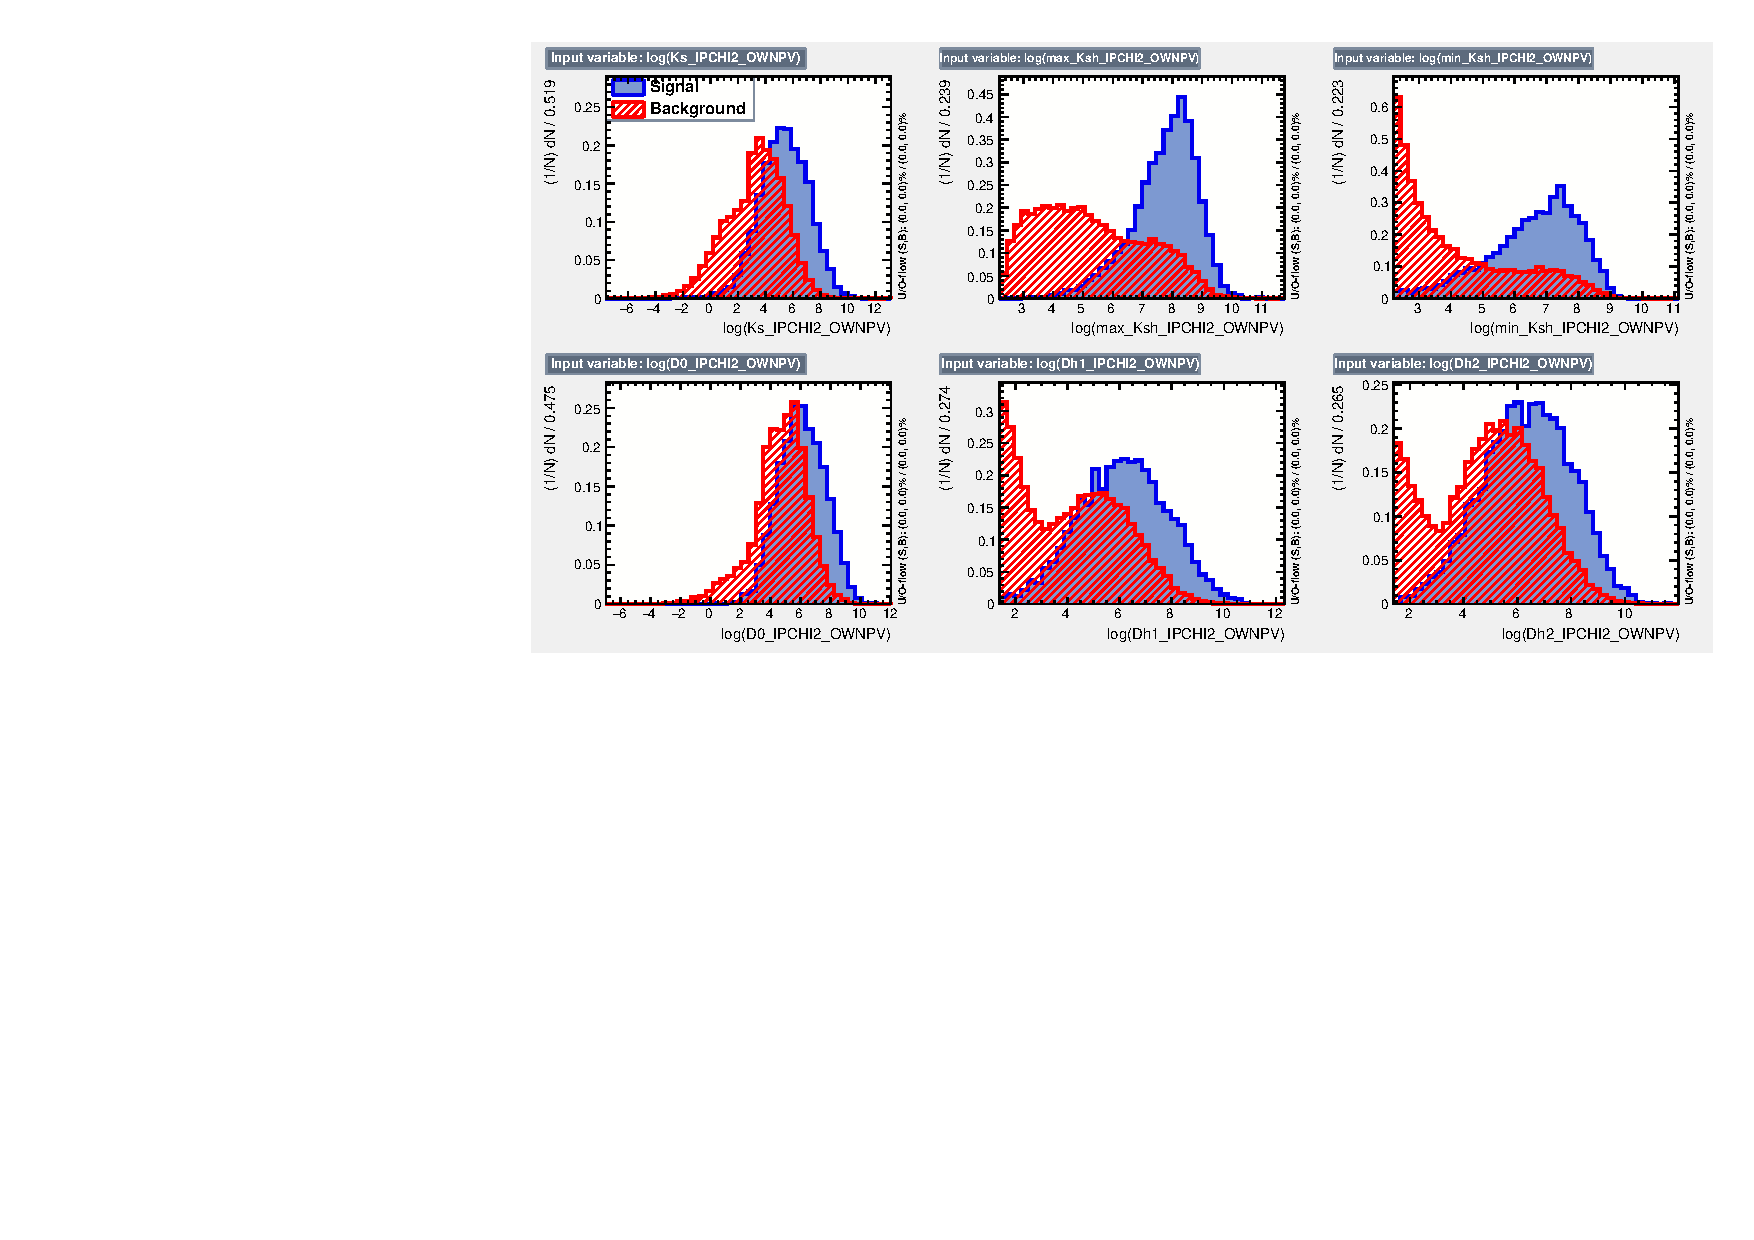
\includegraphics[width=\linewidth]{figures/selection/inputvariables_KPi_LL_run1_1.pdf}
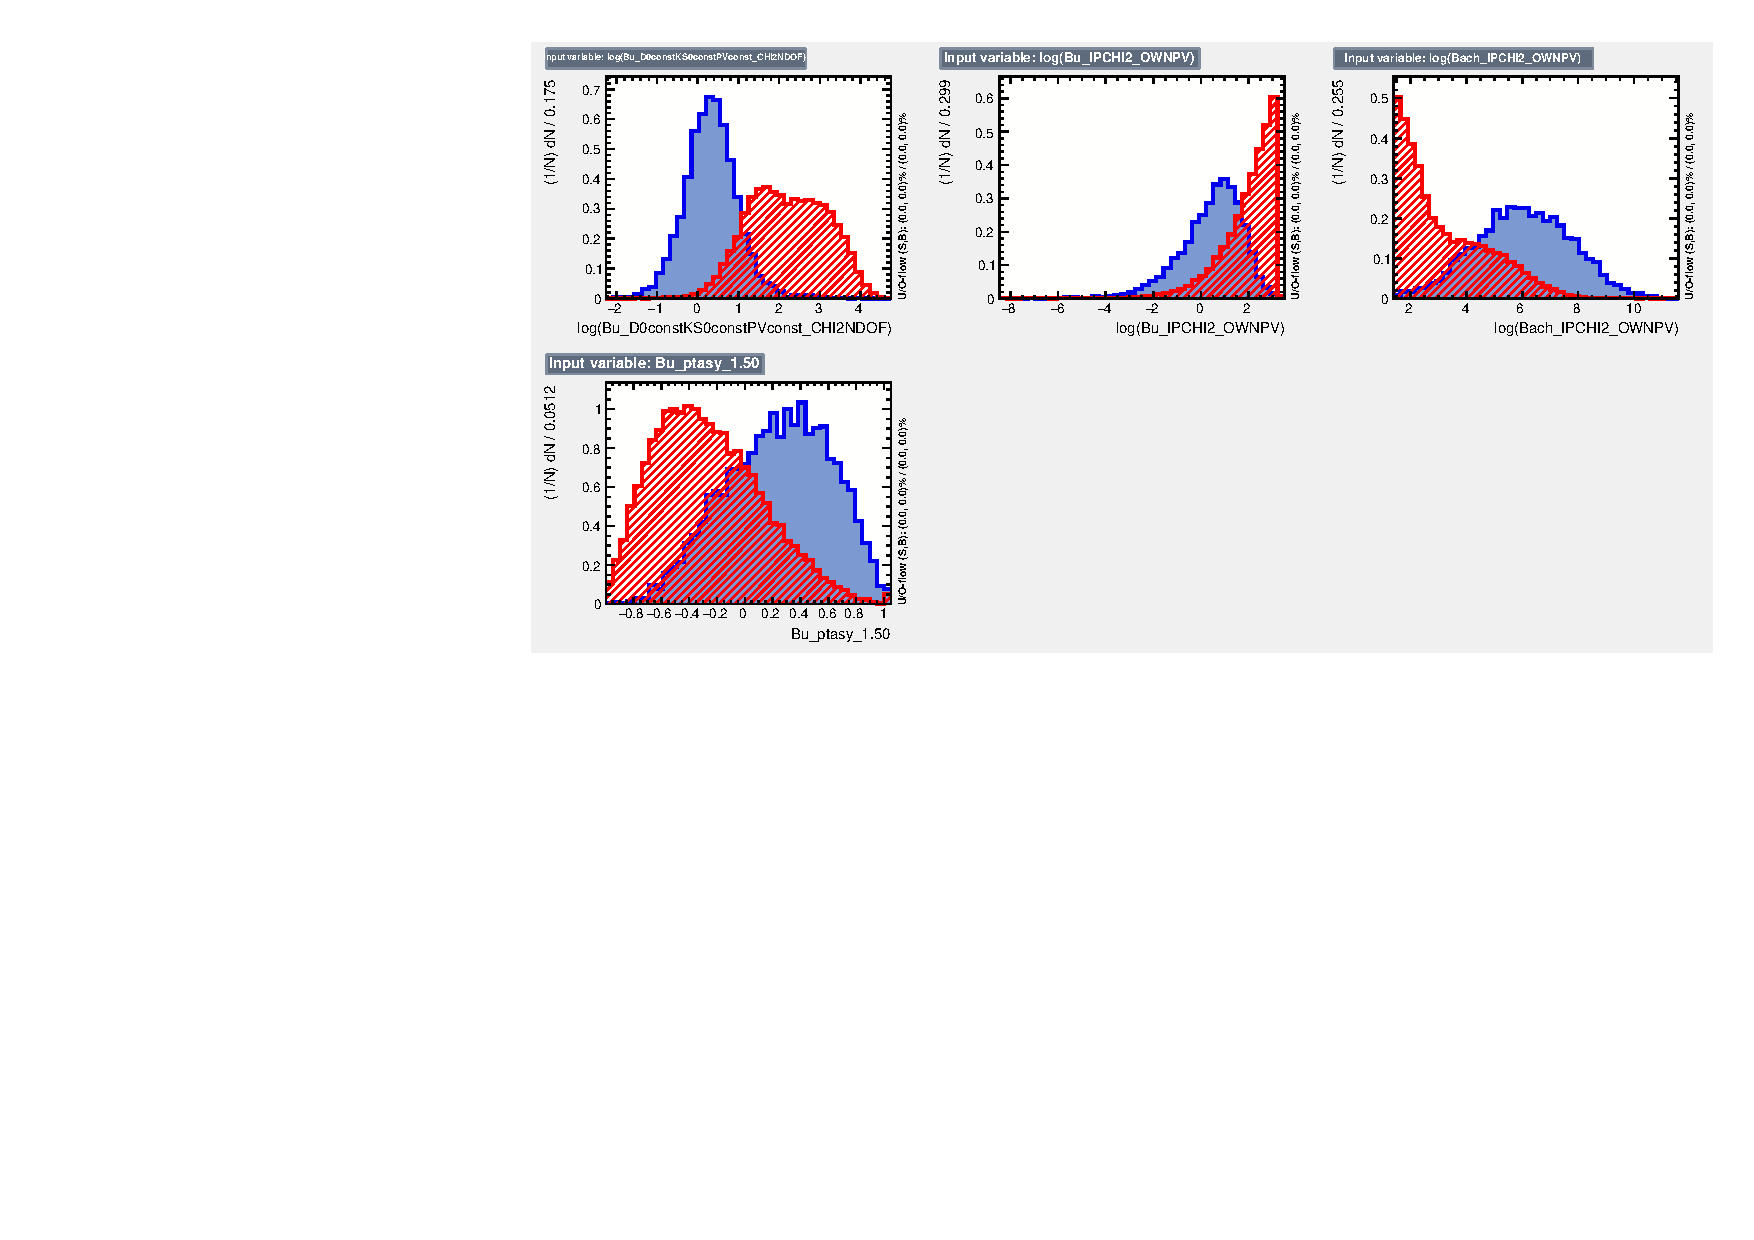
\includegraphics[width=\linewidth]{figures/selection/inputvariables_KPi_LL_run1_2.pdf}
\caption{BDT input variable distributions for signal and background for 2-body LL}
\label{BDTinputdist2bodyLL}
\end{figure}

\begin{figure}[tb]
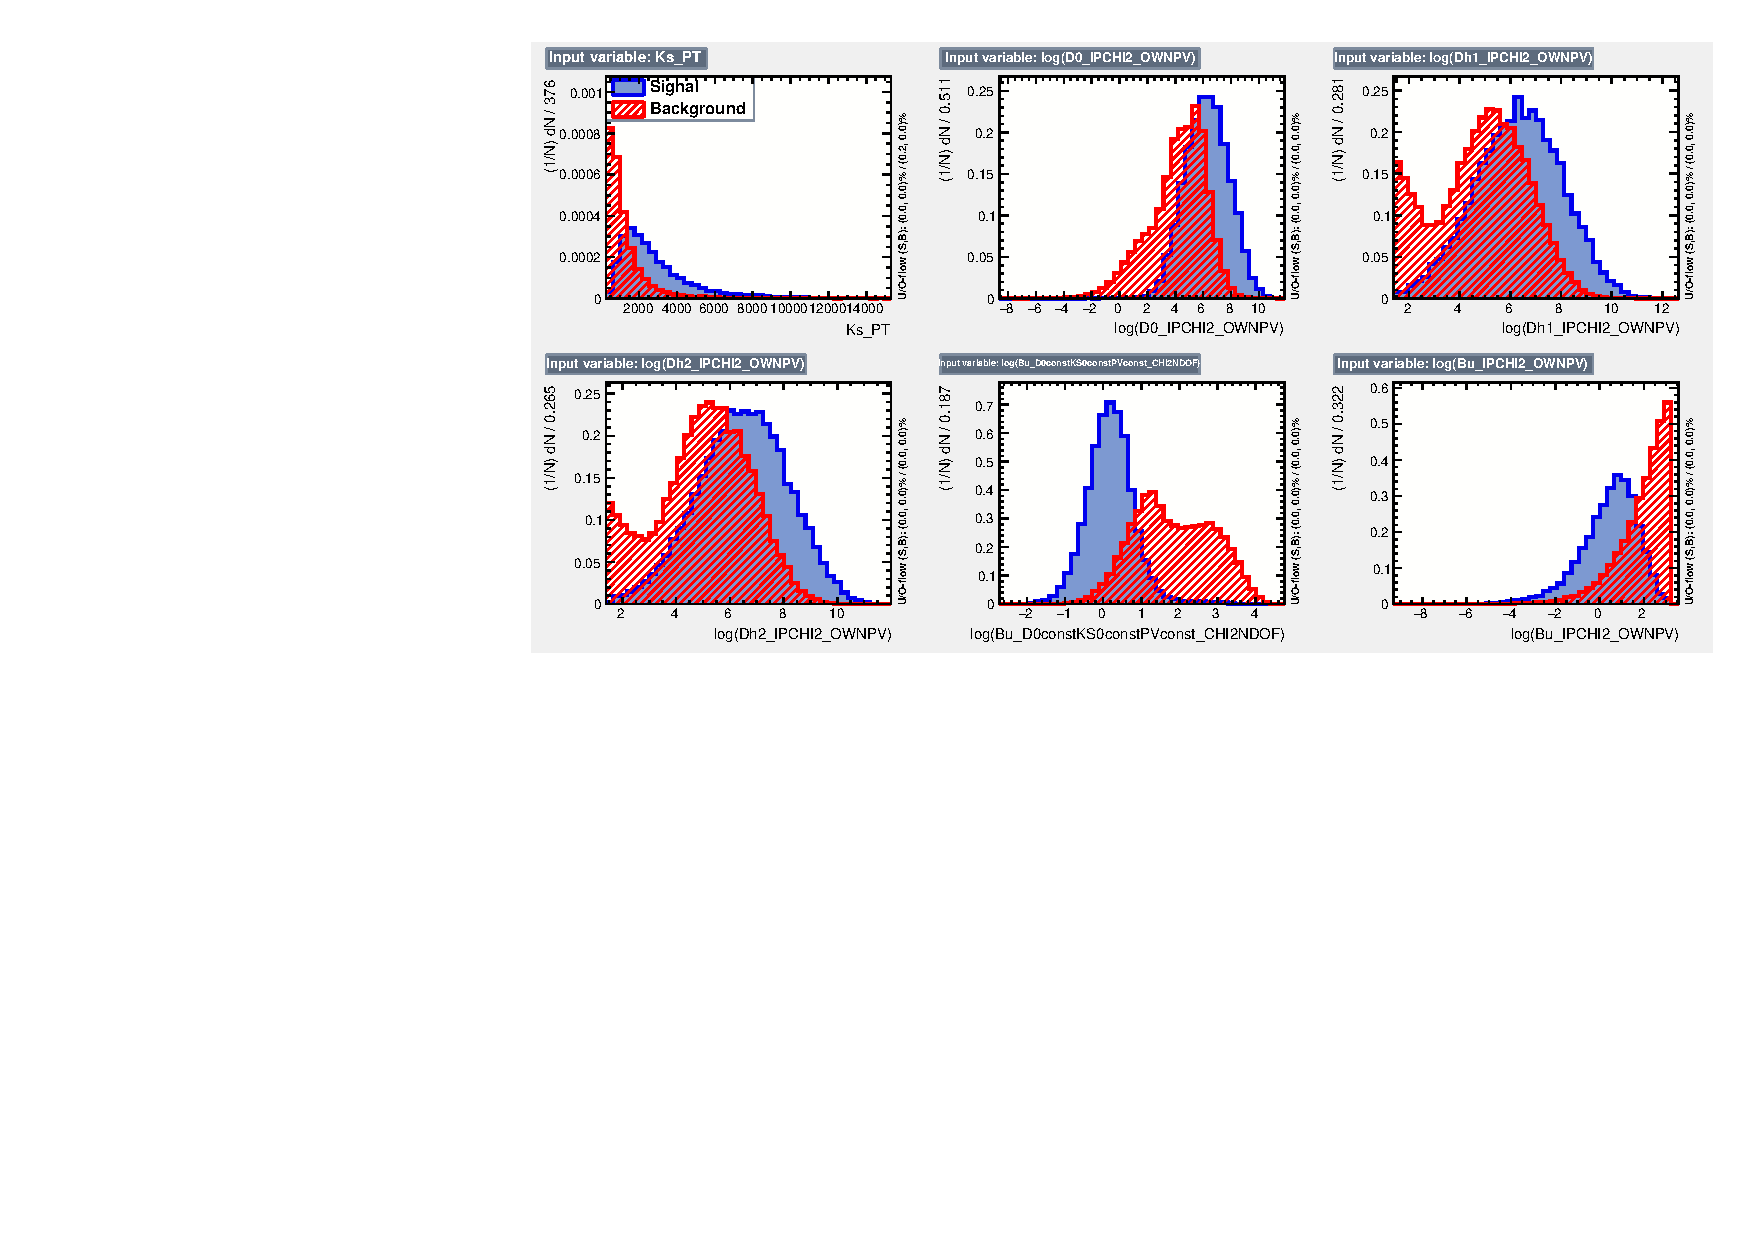
\includegraphics[width=\linewidth]{figures/selection/inputvariables_KPi_DD_run1_1.pdf}
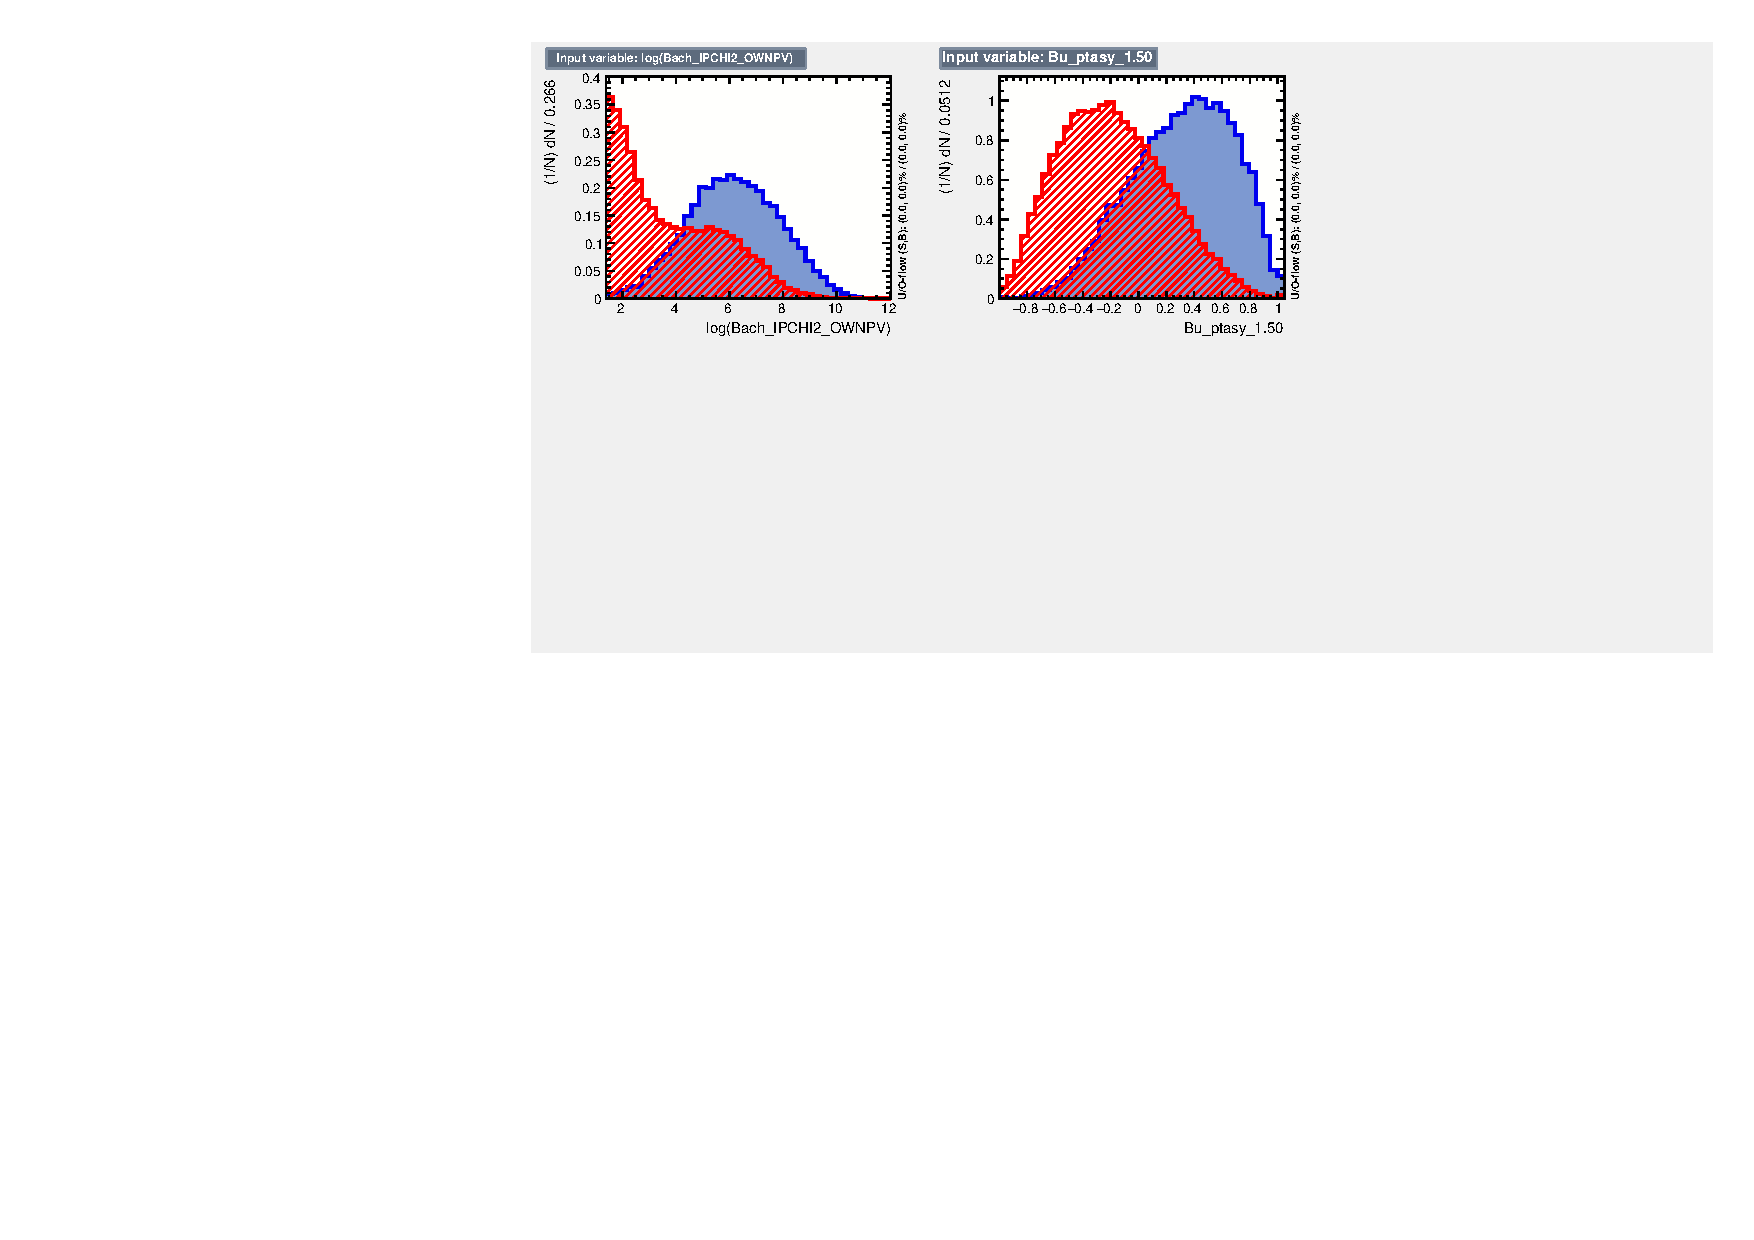
\includegraphics[width=\linewidth]{figures/selection/inputvariables_KPi_DD_run1_2.pdf}
\caption{BDT input variable distributions for signal and background for 2-body DD}
\label{BDTinputdist2bodyDD}
\end{figure}

\begin{figure}[tb]
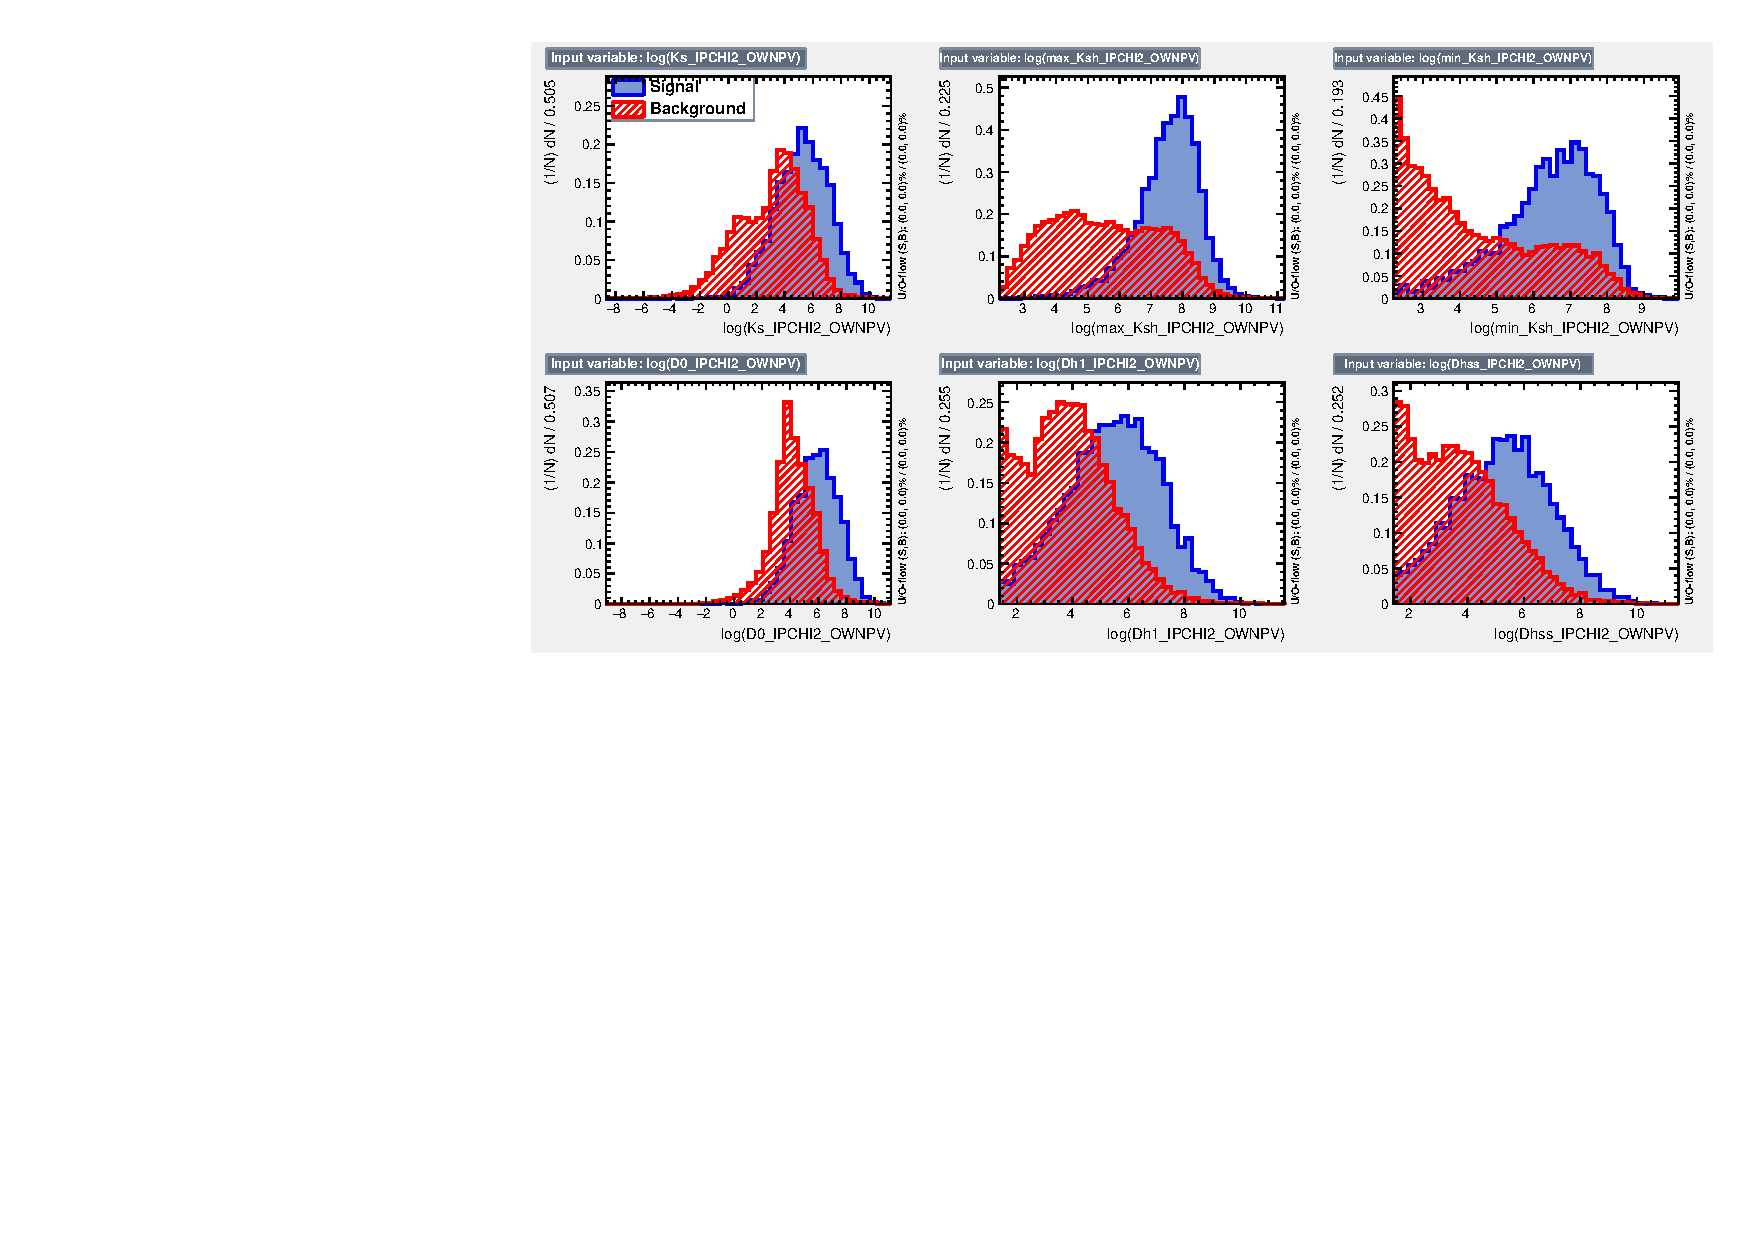
\includegraphics[width=\linewidth]{figures/selection/inputvariables_KPiPiPi_LL_run2_1.pdf}
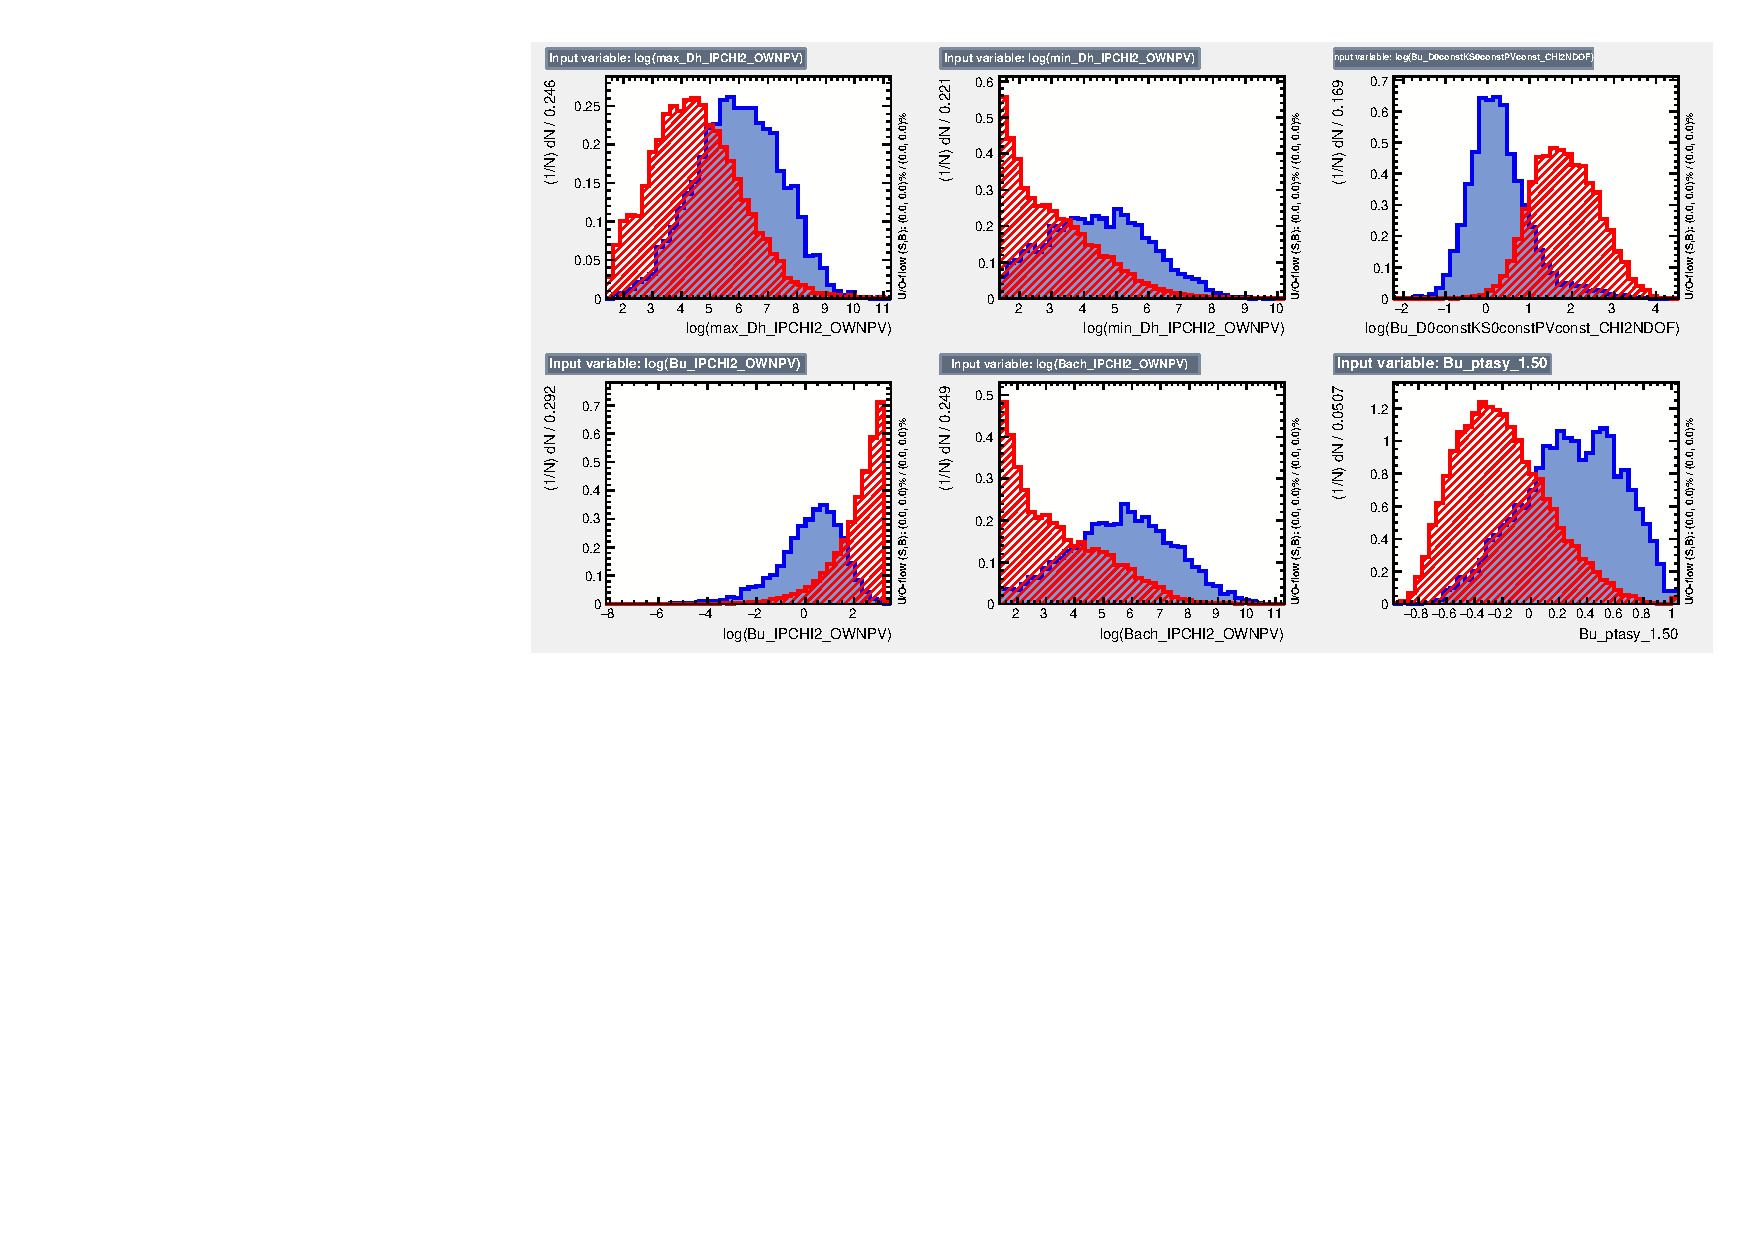
\includegraphics[width=\linewidth]{figures/selection/inputvariables_KPiPiPi_LL_run2_2.pdf}
\caption{BDT input variable distributions for signal and background for 4-body LL}
\label{BDTinputdist4bodyLL}
\end{figure}

\begin{figure}[tb]
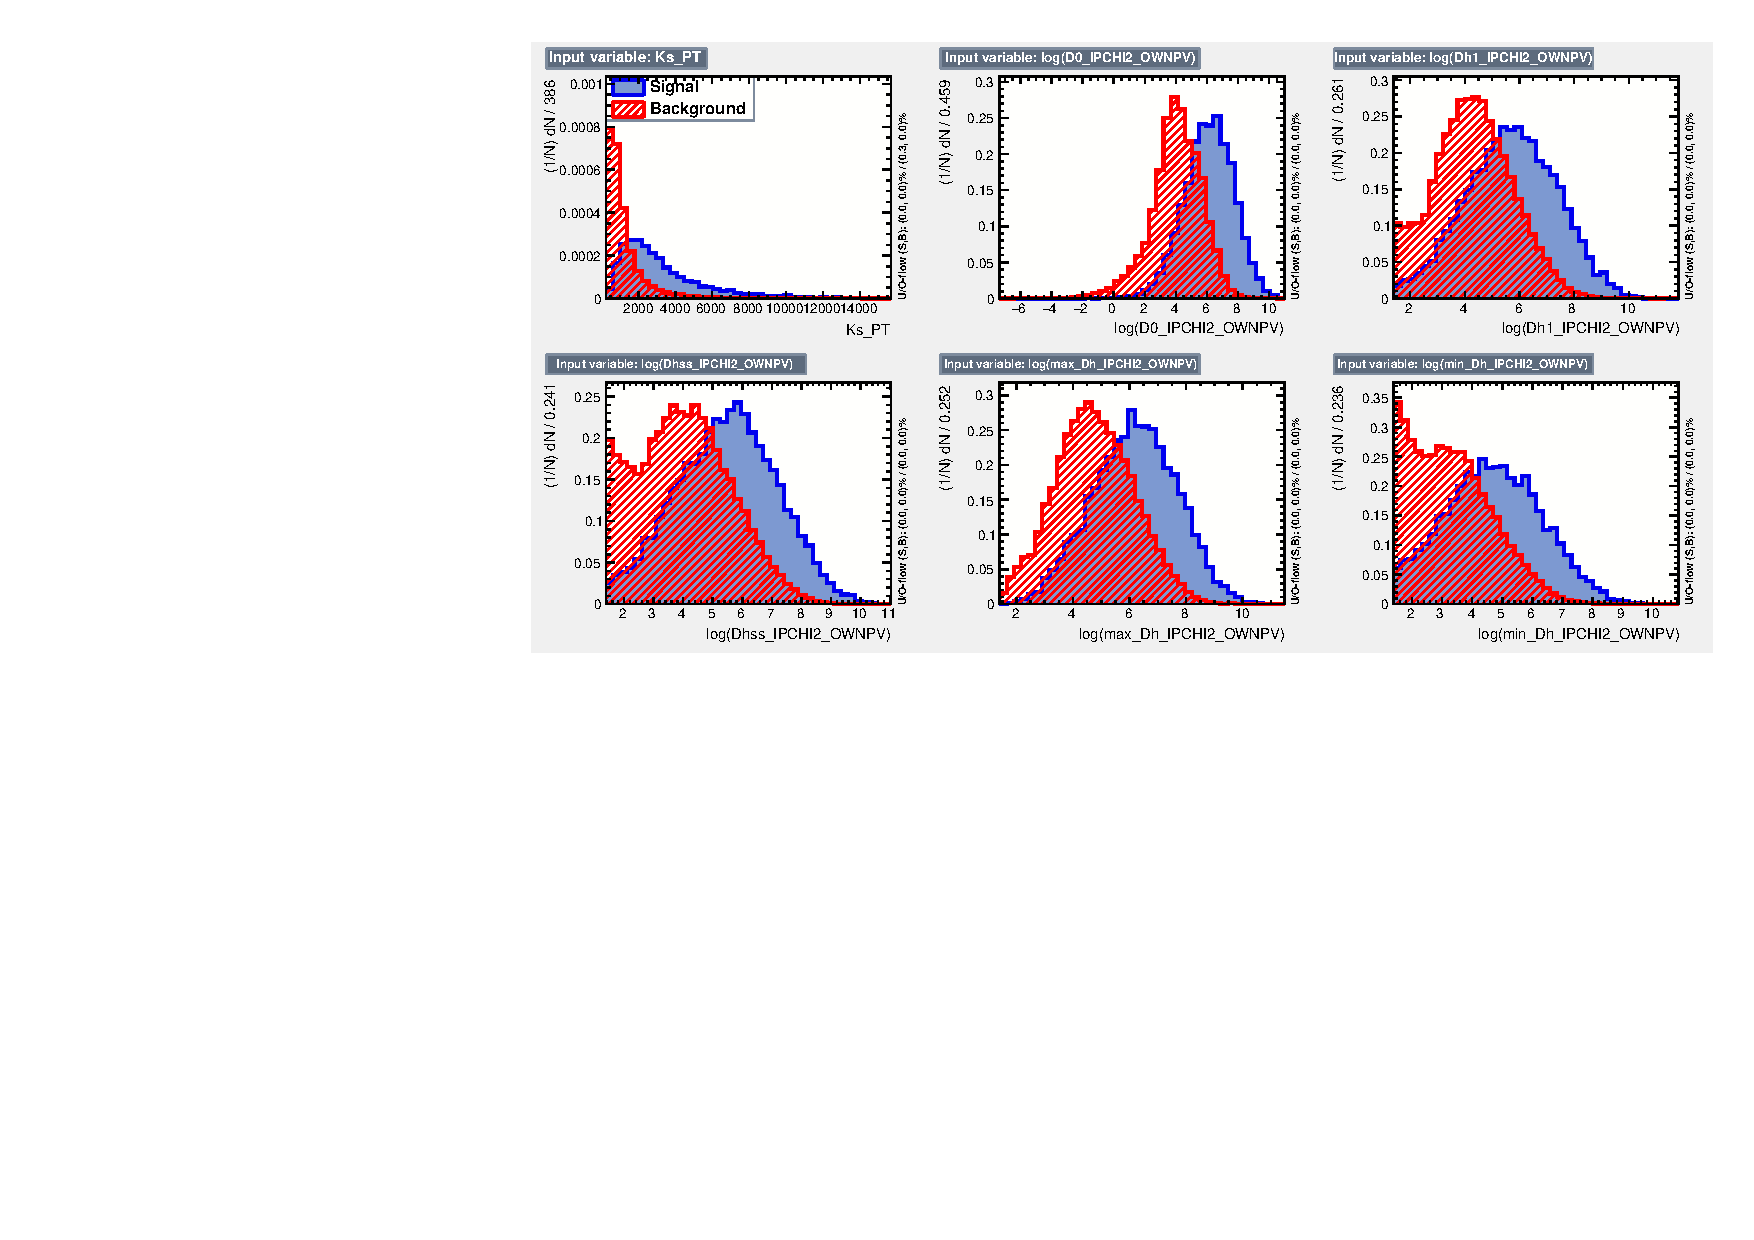
\includegraphics[width=\linewidth]{figures/selection/inputvariables_KPiPiPi_DD_run2_1.pdf}
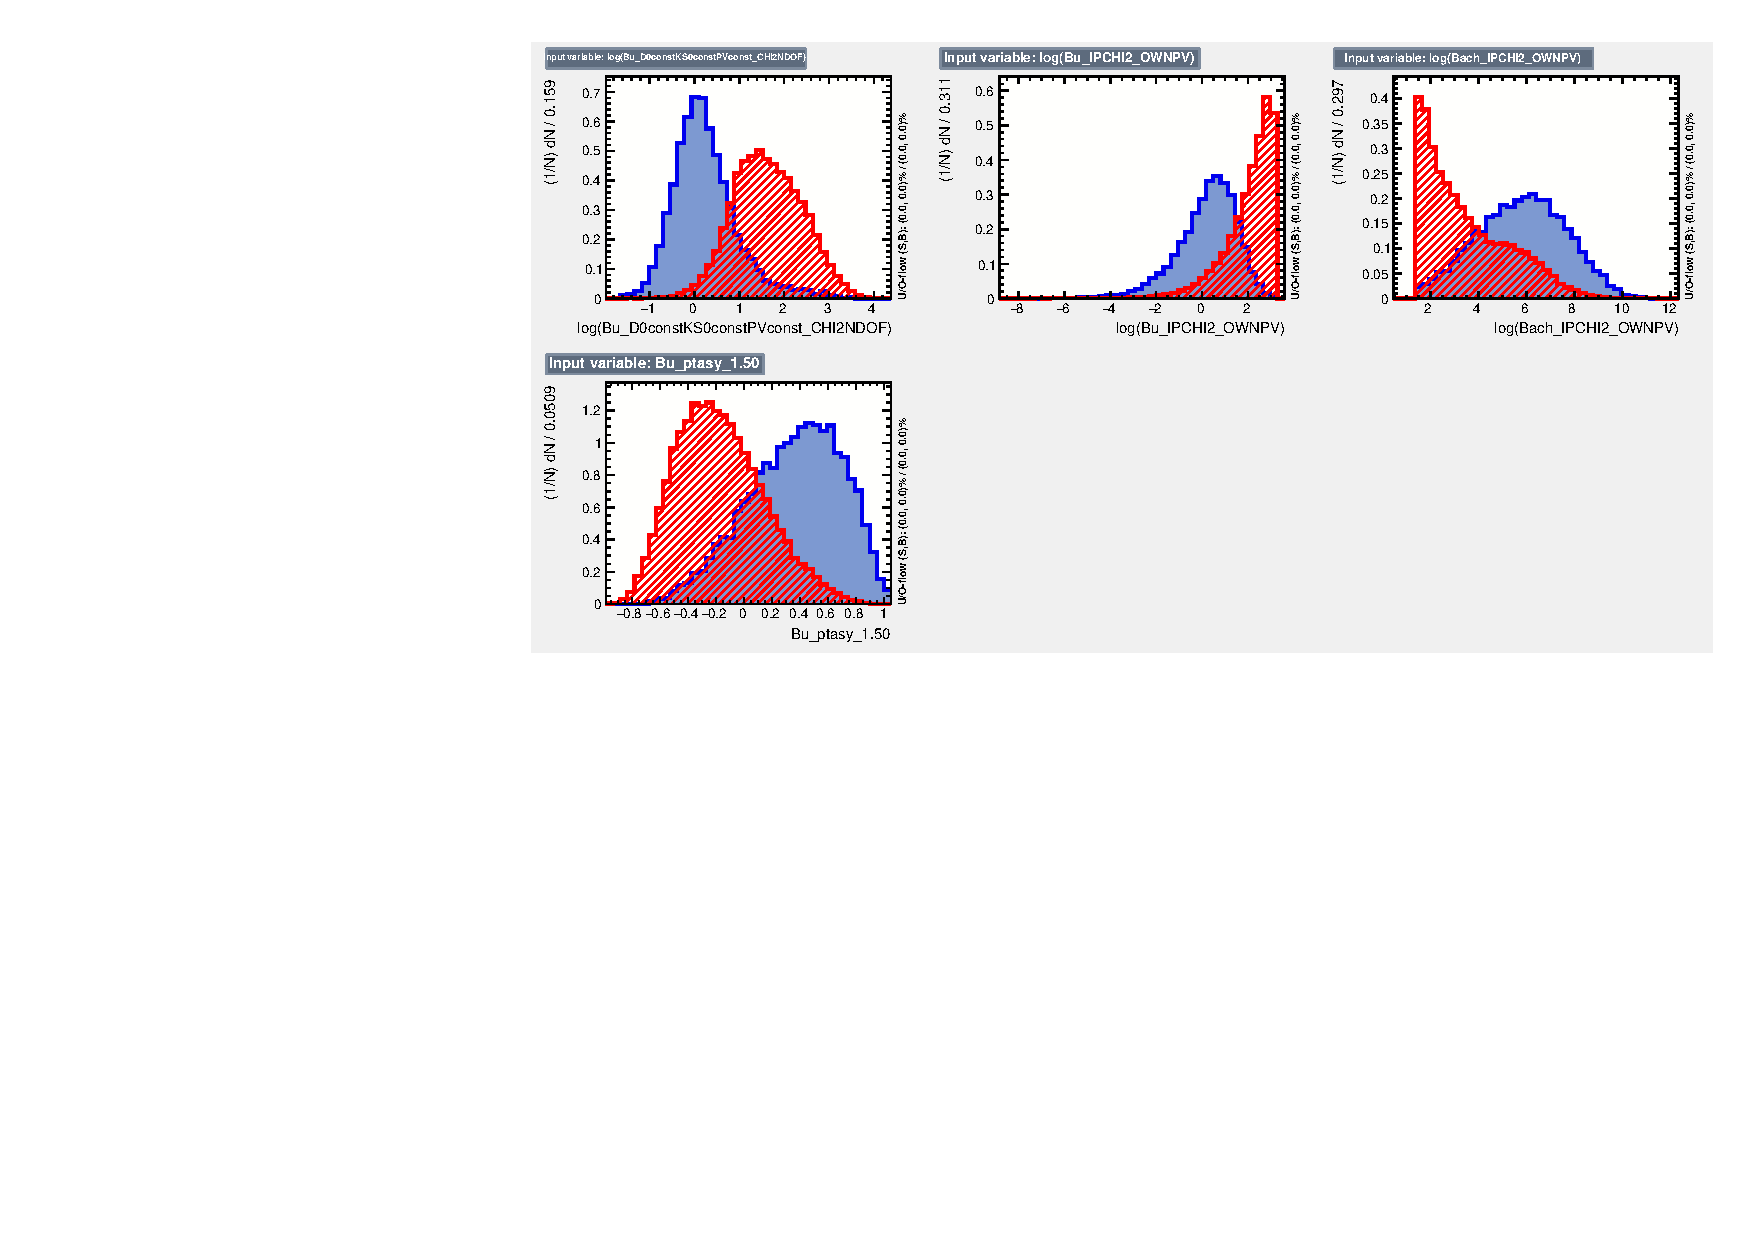
\includegraphics[width=\linewidth]{figures/selection/inputvariables_KPiPiPi_DD_run2_2.pdf}
\caption{BDT input variable distributions for signal and background for 4-body DD}
\label{BDTinputdist4bodyDD}
\end{figure}

\begin{figure}[tb]
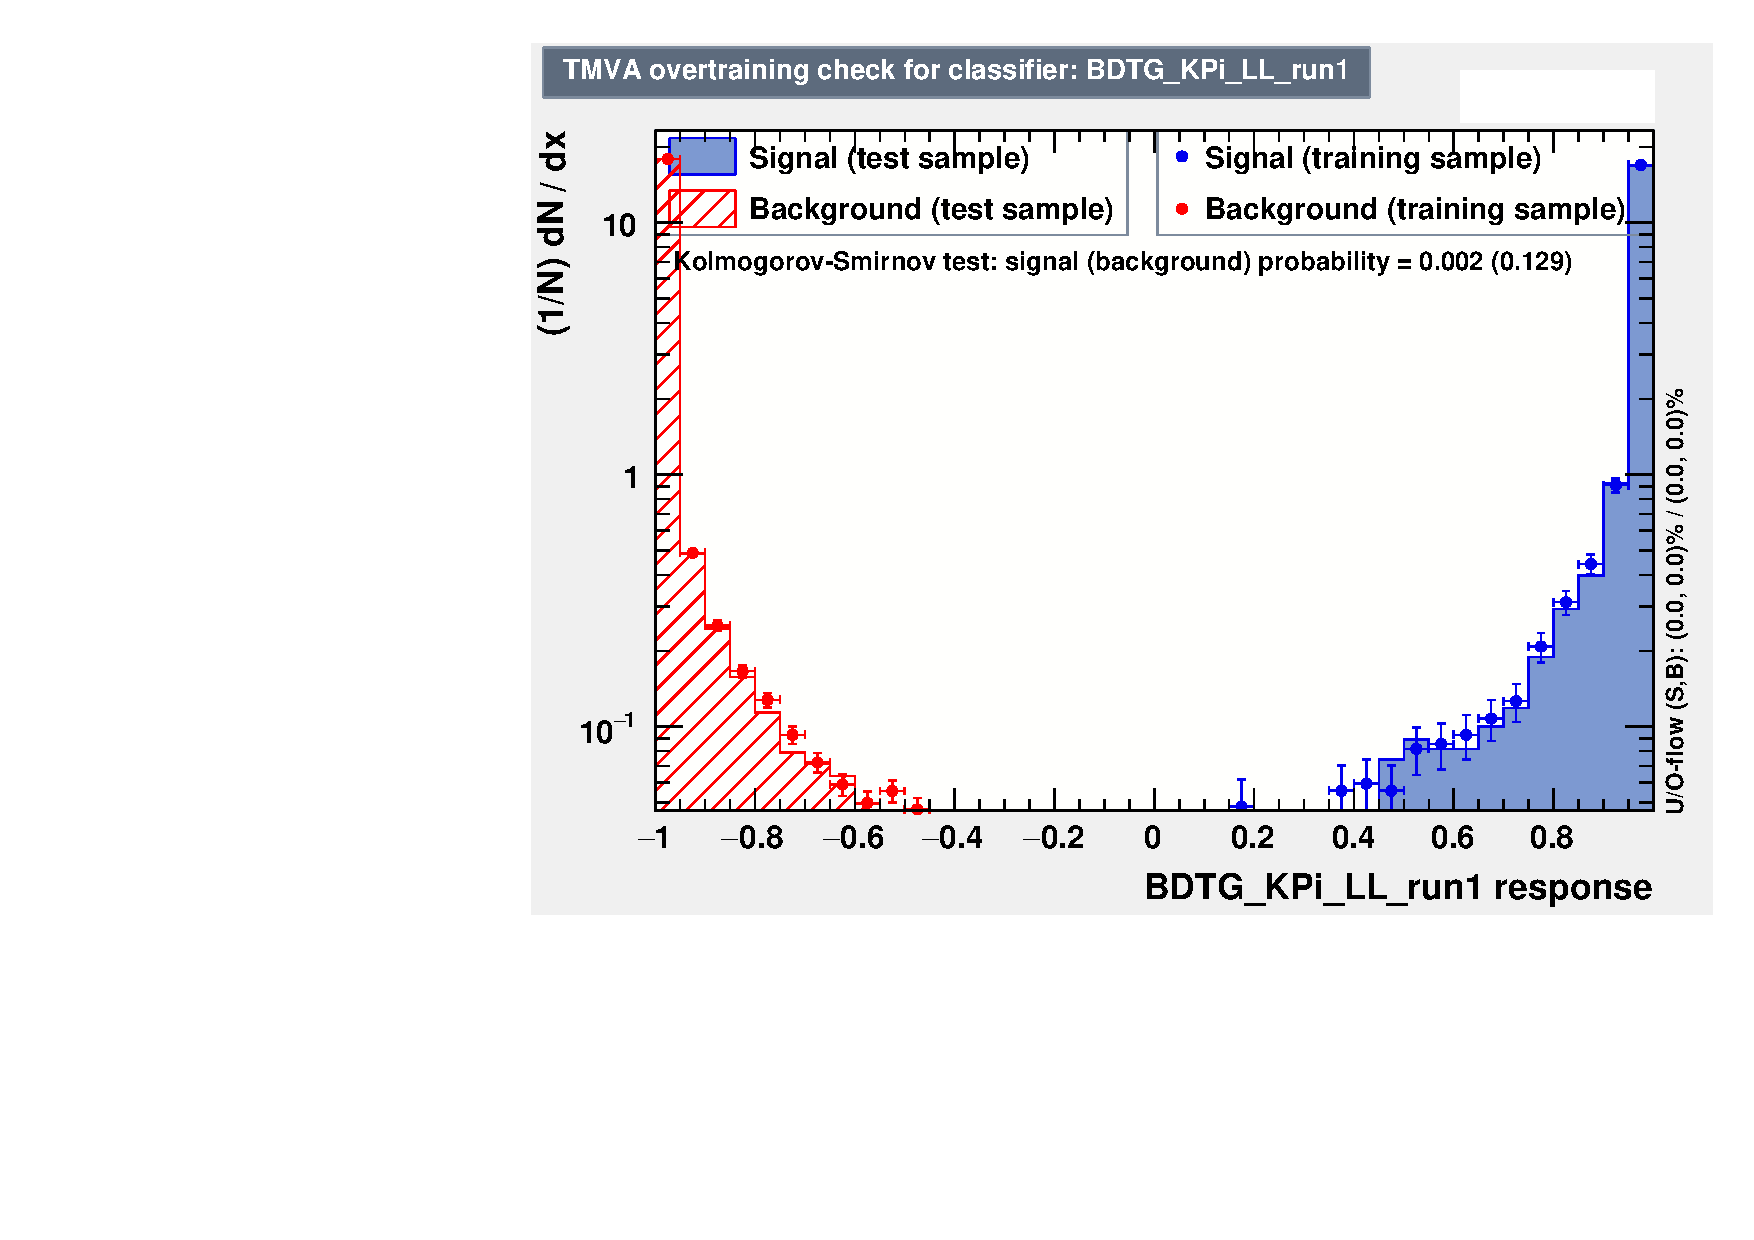
\includegraphics[width=0.5\linewidth]{figures/selection/overtraining_KPi_LL_run1.pdf}
\put(-150,100) {(a)}
\hfill
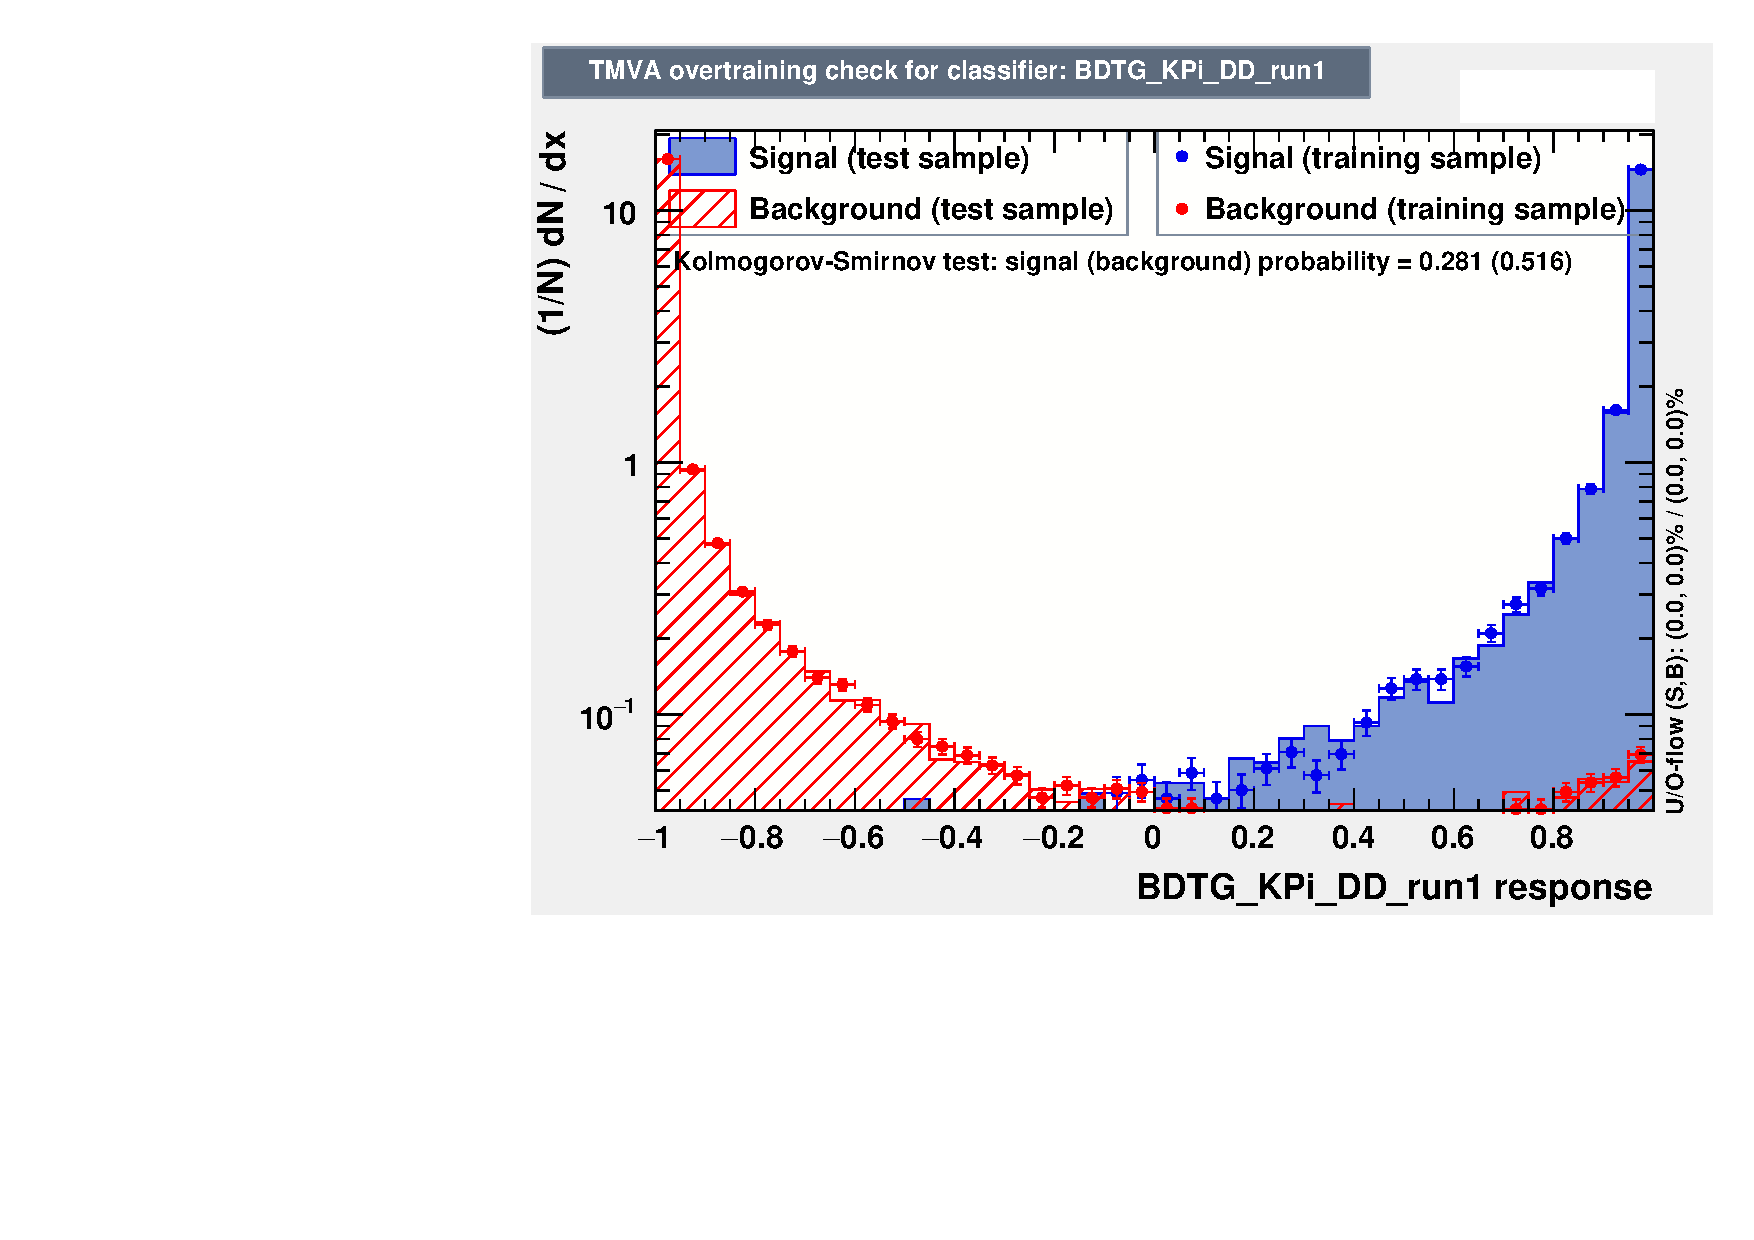
\includegraphics[width=0.5\linewidth]{figures/selection/overtraining_KPi_DD_run1.pdf}
\put(-140,100) {(b)}
\hfill
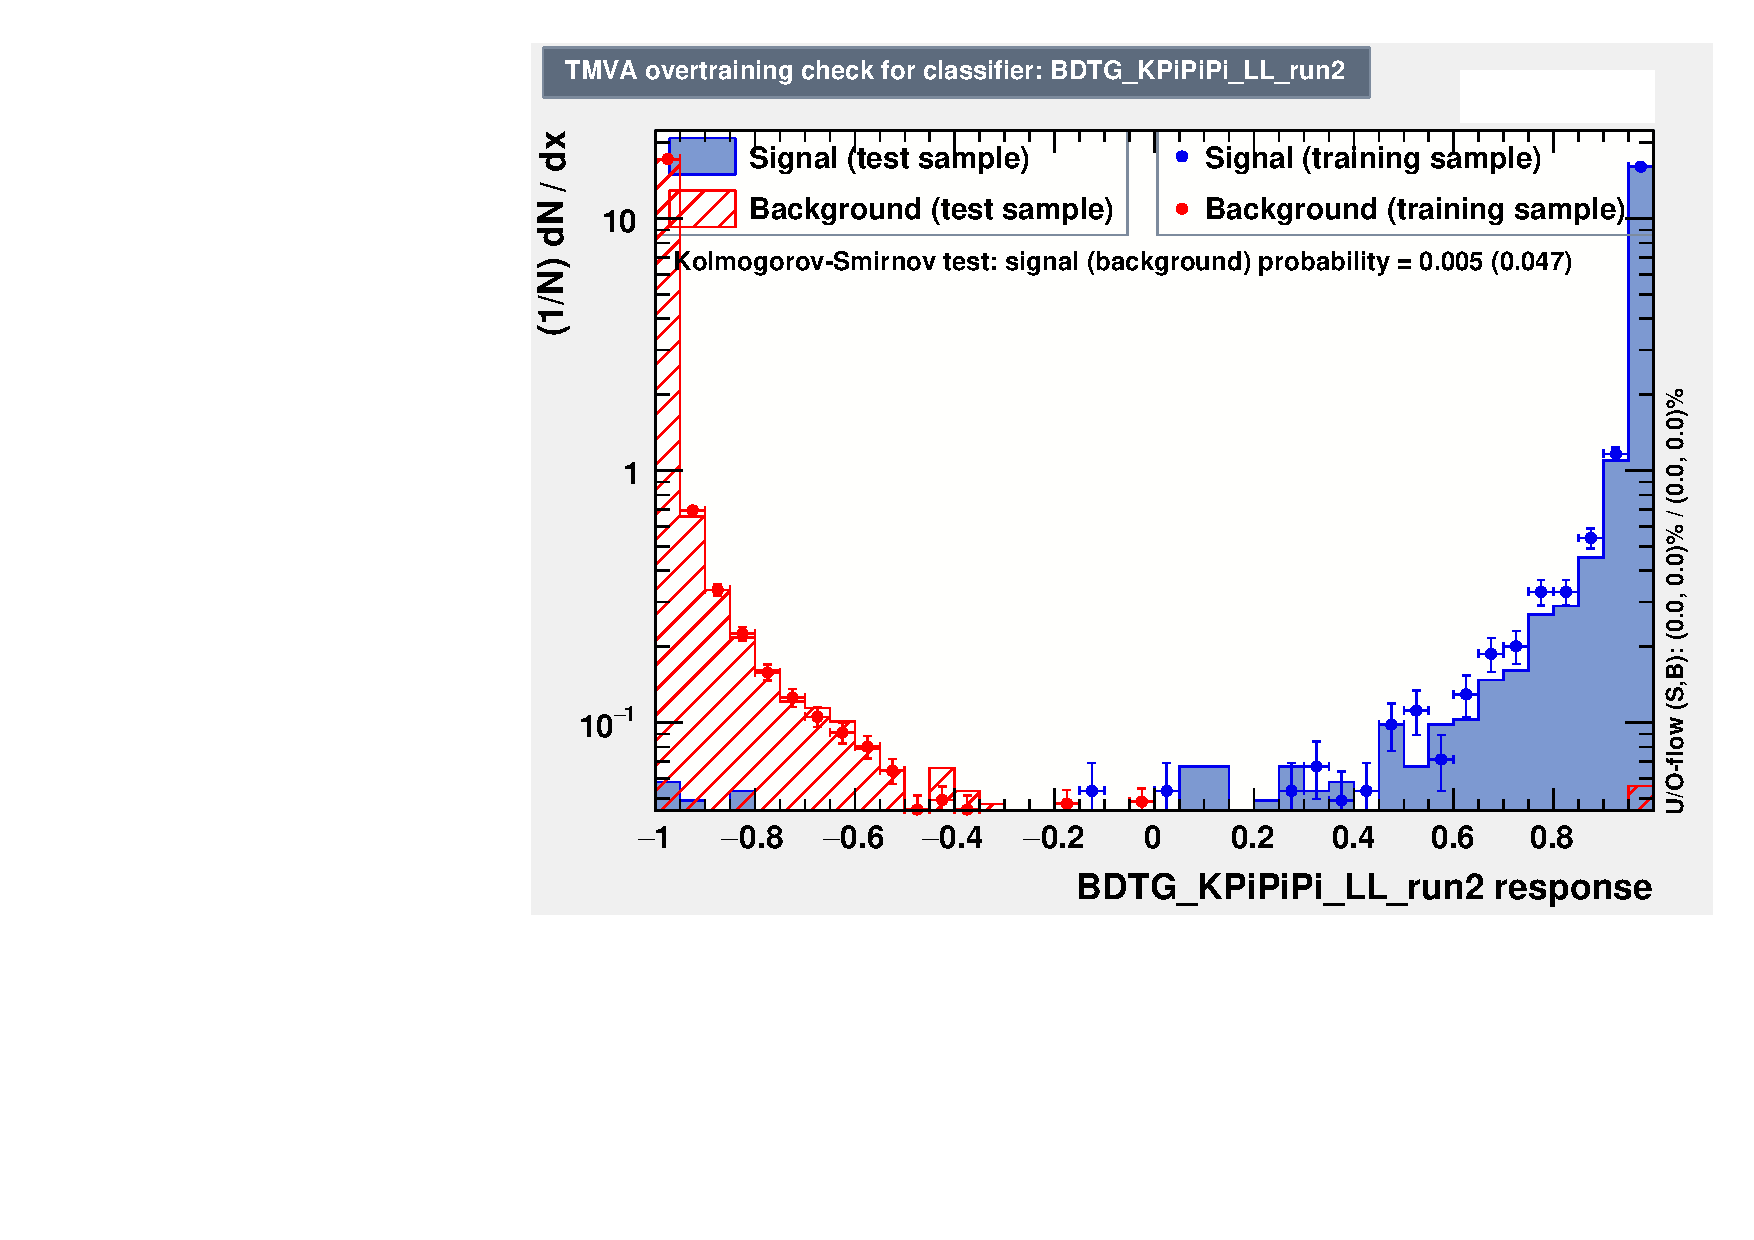
\includegraphics[width=0.5\linewidth]{figures/selection/overtraining_KPiPiPi_LL_run2.pdf}
\put(-150,100) {(c)}
\hfill
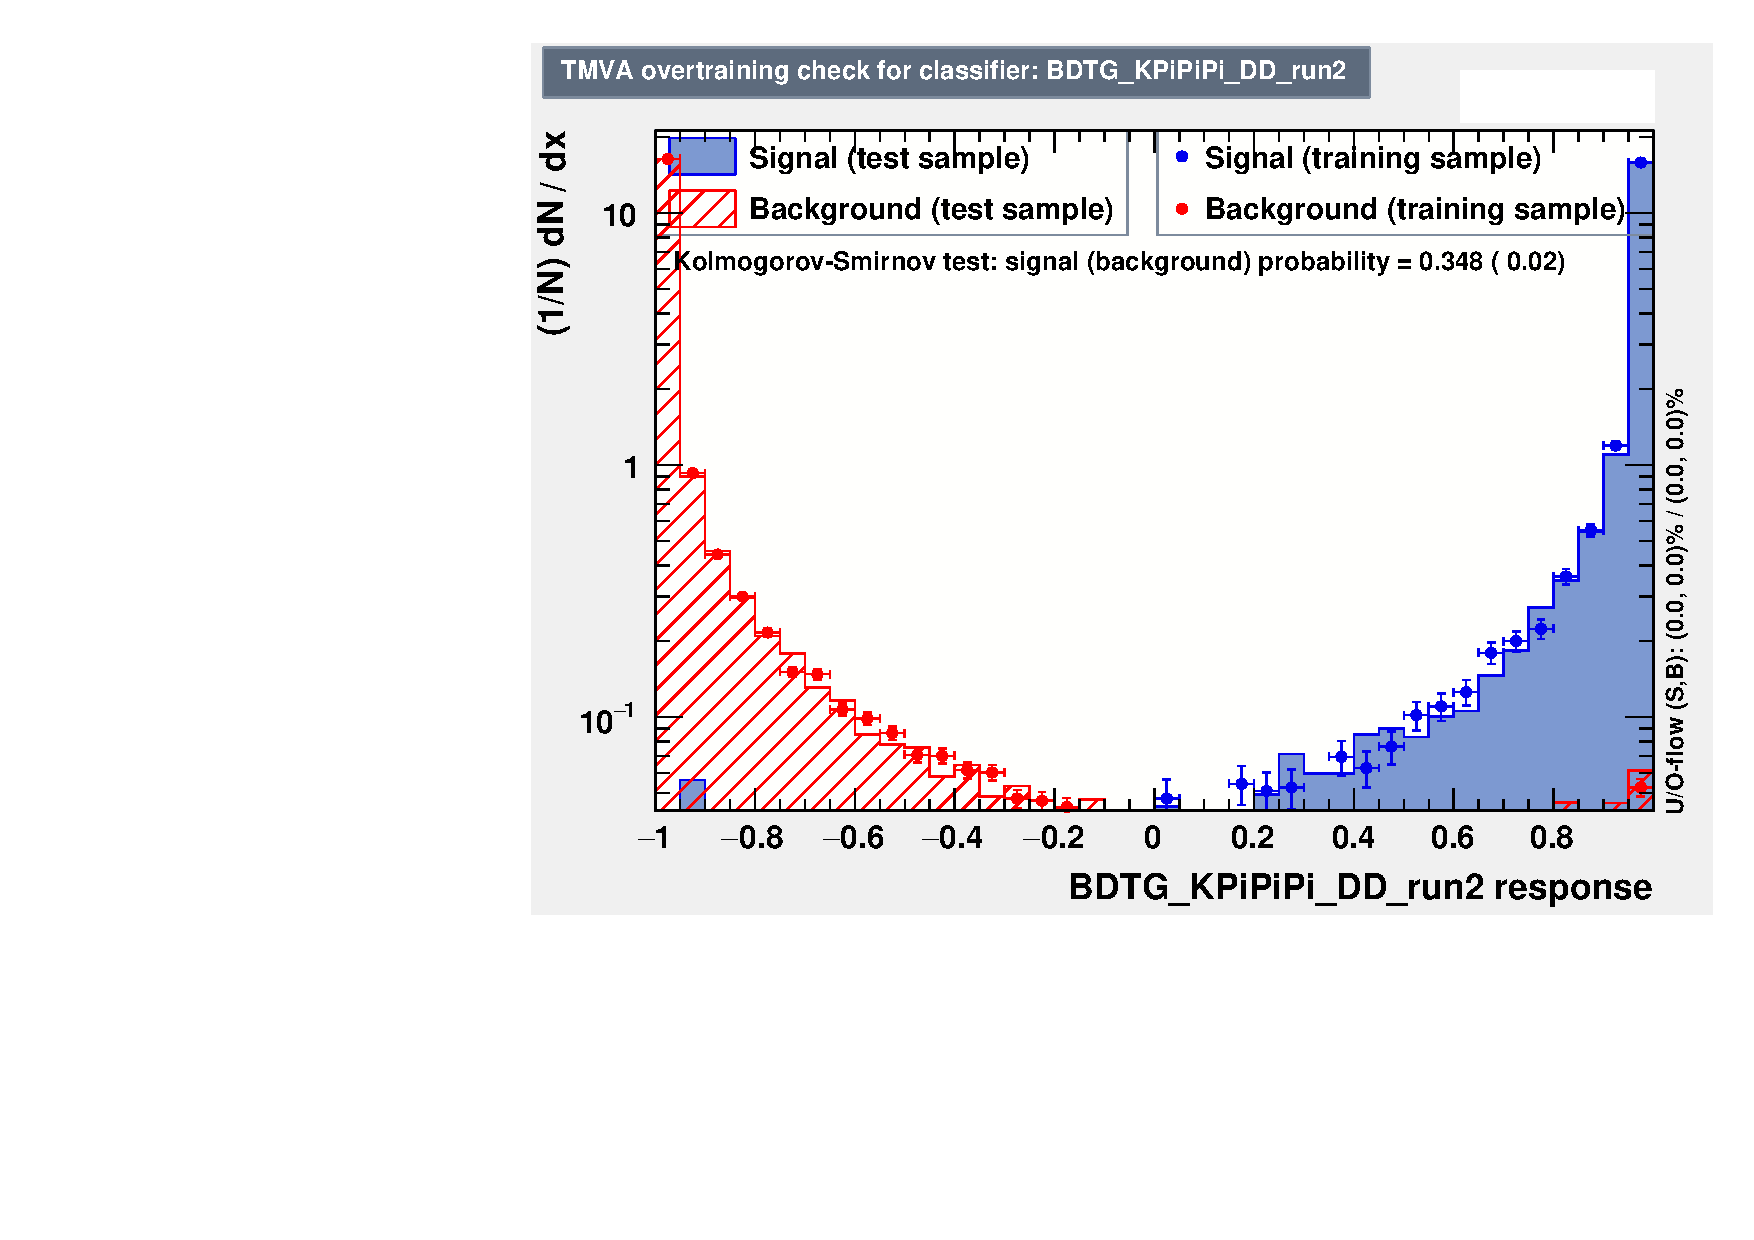
\includegraphics[width=0.5\linewidth]{figures/selection/overtraining_KPiPiPi_DD_run2.pdf}
\put(-140,100) {(d)}
\caption{Training and test distributions from TMVA for (a) 2-body BDT\_LL, (b) 2-body BDT\_DD, (c) 4-body BDT\_LL and (d) 4-body BDT\_DD}
\label{BDTovertraining}
\end{figure}

Other selection strategies were explored. Multiple BDTs were investigated, by training and implementing a \KS BDT and a \Dz BDT followed by a B BDT. Two approaches were tried: one using the same set of variables in all three BDTs and one using variables relating to the \KS in the \KS BDT and variables relating to the \Dz in the \Dz BDT. These methods were found to have little or no improvement on the single BDT. Many other variables were investigated in the BDT, including kinematic variables of the \B and \D. These were found to give no significant improvement in BDT performance. A two-body BDT trained on Run 2 data and simulation was investigated to apply to Run 2 data, which did not result in any improvement in performance compared to the BDT trained on Run 1. Therefore, it was not considered necessary to have BDTs trained separately for Run 1 and Run 2.

\subsubsection{BDT performance and choice of working point}

The results obtained from training are applied to the testing sample in order to check for overtraining, which occurs when the classifier has learned statistical fluctuations present in the training sample. The results are shown in Figure \ref{BDTovertraining}. The training and testing distributions are in reasonable agreement, showing that the BDT is safe from overtraining effects.

The BDT selections, in conjuction with the \Kstarm mass window and \KS helicity angle, were optimised to reduce the fit error on the physics observables, as detailed in Section \ref{sec:cpfit:optimisation}. Many toy studies were run to calculate the fit uncertainty for each selection. To optimise the selection for the GLW modes, the fit error was minimised for $A_{KK}$, $R_{KK}$, $A_{\pi\pi}$ and $R_{\pi\pi}$. The BDT selection for the ADS modes was optimised to minimise the fit errors in $R^+$ and $R^-$, as illustated in Figure \ref{adsoptimisation}. In cases when the figure of merits in these optimisation studies were not especially sensitive to changes in the selection, the selection giving the highest coherence (i.e most stringent requirement on the \Kstarm) was chosen and the BDT signal and background efficiencies were taken into account.

For the two-body BDTs, a BDT selection of 0.6 is chosen for BDT\_LL and 0.7 for BDT\_DD for all D modes except the ADS mode. The ADS mode BDT selection is chosen to be 0.6 for BDT\_LL and 0.9 for BDT\_DD. This tighter BDT selection is justified in Figure \ref{adsoptimisation}. When applied to the $K\pi$ favoured mode in Run 1 the BDT selection gives a 95\% signal efficiency and 96\% background rejection for LL and 88\% signal efficiency and 94\% background rejection for DD. 

For the four-body modes the same optimisation point was chosen 0.6 for BDT\_LL and 0.7 for BDT\_DD for the \decay{\Dz}{\Kp\pim\pip\pim} \decay{\Dz}{\pi\pi\pi\pi} mode, and 0.6 for BDT\_LL and 0.9 for BDT\_DD for the \decay{\Dz}{\Kp\pim\pip\pim} mode. The optimisation point was verified by minimising the fit error in toys for $A_{K\pi\pi\pi}$, $R^+_{K\pi\pi\pi}$ and $R^-_{K\pi\pi\pi}$. The signal efficiencies of the BDT selection is given in Table \ref{bdteff}. 


\subsection{Other cuts}

Some other selection requirements are implemented to isolate the signal candidates and tackle certain backgrounds.

Figure \ref{helicitycut} shows that the MC distribution of the cosine of Ks helicity angle is asymmetric. Physically the Ks helicity angle is expected to follow a symmetric $cos^2\theta$ distribution, however the observed asymmetry in this variable, manifest in both data and MC, was found to be due to the momentum and transverse momentum cuts placed on the bachelor pion in the stripping line. Figure \ref{helictyasymmetry} illustrates this point.

\begin{figure}[h]
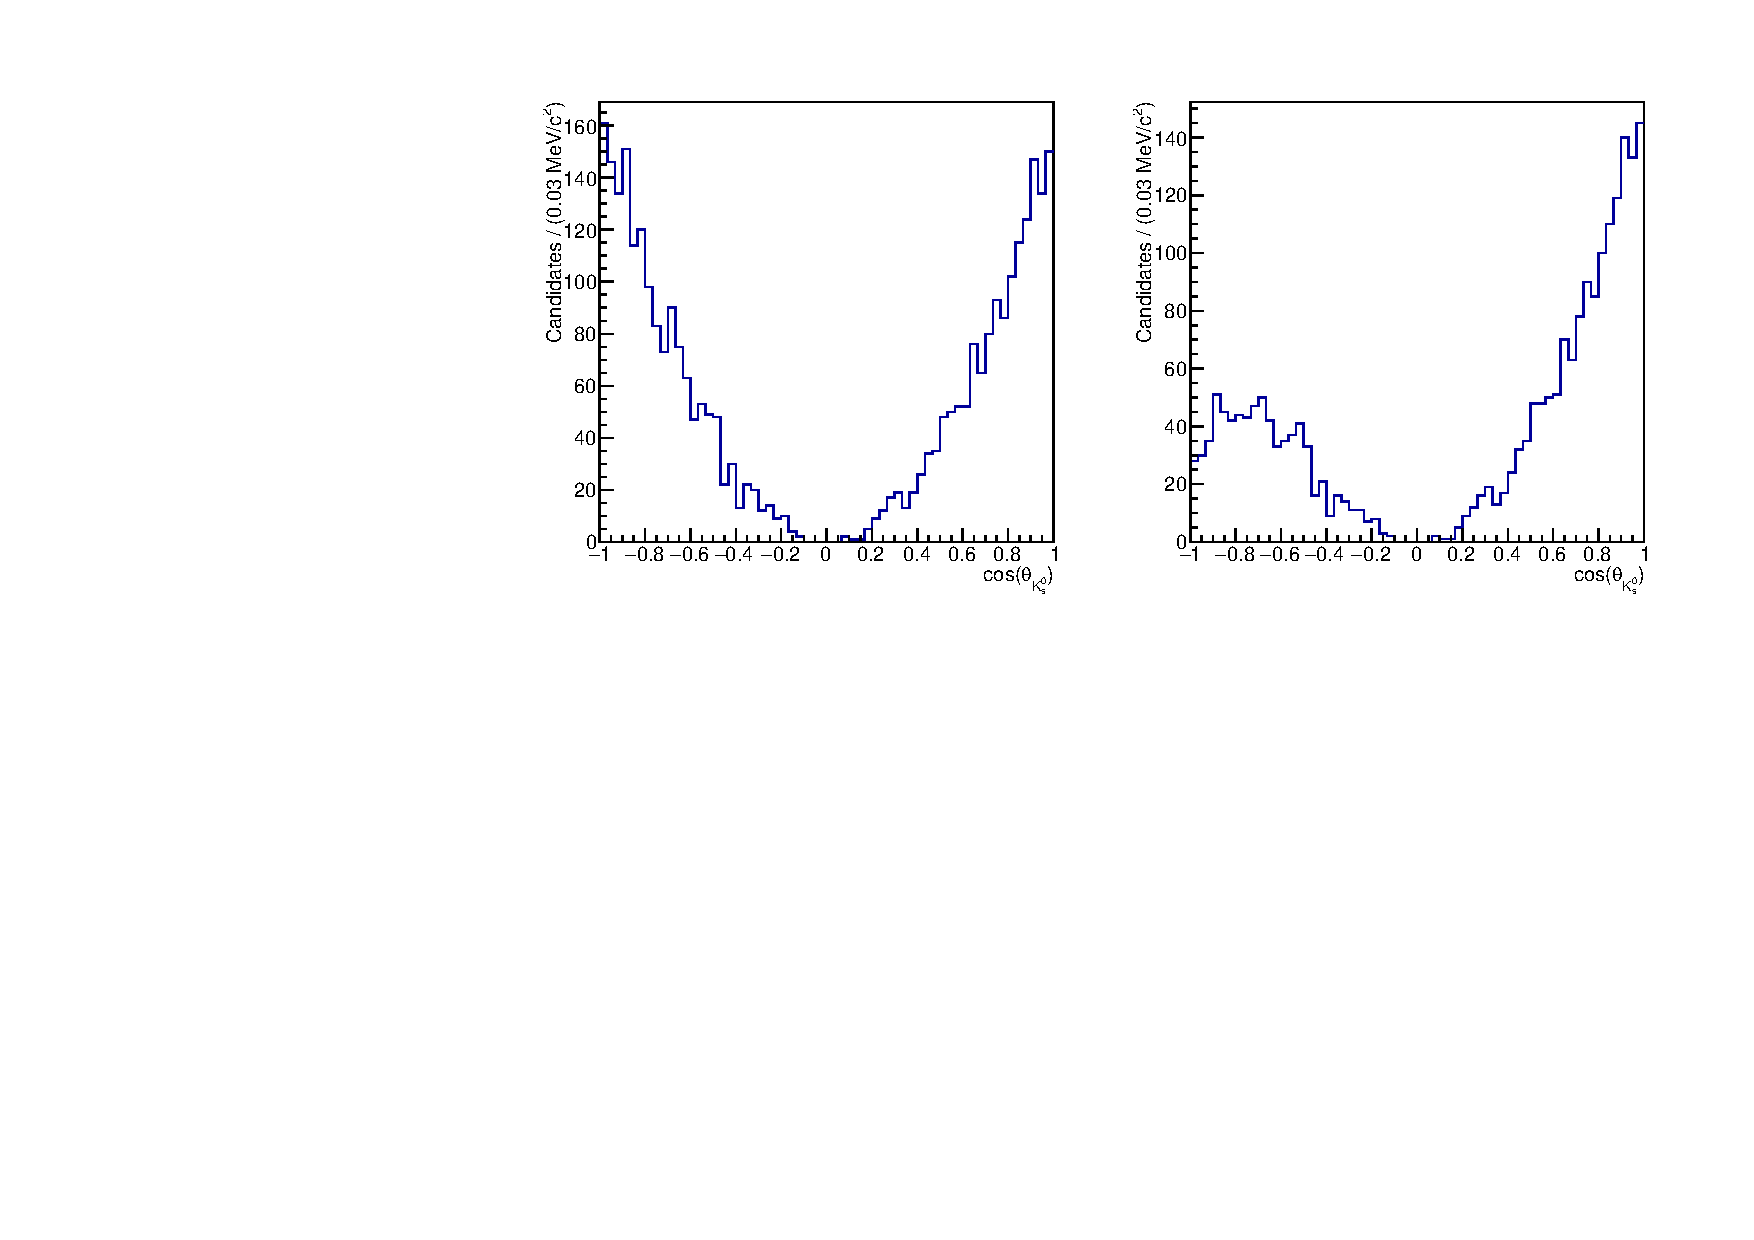
\includegraphics[width=\linewidth]{figures/helicityAngleAsymmetry.pdf}
\put(-360,150) {(a)}
\put(-150,150) {(b)}
\caption{\KS helicity angle MC distribution at generator level with (a) no cuts applied, and (b) bachelor $p > 2500$ MeV and bachelor $p_T > 250$ MeV, as in the stripping line}
\label{helictyasymmetry}
\end{figure}

\begin{itemize}
\item The reconstructed \Dz mass must lie within 25 \mev of the known \Dz mass
\item The reconstructed \Kstarm mass must lie within 75 \mev of the known \Kstarp mass
\item{\textbar $\cos$(Ks helicity angle) \textbar $>$ 0.3, discussed in Section \ref{sec:backgrounds:non-resonant}. This angle is defined as is the angle between the \KS and the bachelor pion in the \Kstarm rest frame}
\item{\Dz FD significance $>$ 2 is required to remove charmless backgrounds, discussed in Section \ref{sec:backgrounds:charmless}}
\item{\KS FD significance $>$ 5 (for LL candidates only) is required to remove $B \to D\pi\pi\pi$ background, discussed in Section \ref{sec:backgrounds:b2dpipipi}}
\item{15 MeV double misID veto, discussed further in Section \ref{sec:backgrounds:crossfeed}}
\begin{itemize}
\item For two-body: 15 MeV double misID veto is applied to $B^{\pm} \to [K^{\mp}\pi^{\pm}] K^{*\pm}$ only. The \Dz mass is reconstructed where both daughter mass hypotheses are swapped (kaon reconstructed as a pion and pion reconstructed as a kaon), this is required to be greater than 15 MeV away from the nominal \Dz mass.
\item For four-body: There are two possible pions that could be incorrectly reconstructed as a kaon, therefore two 15 MeV double misID vetos are applied to both the favoured and the supressed modes. 
\end{itemize} 
\end{itemize}

\subsection{Studies of peaking backgrounds}
\label{sec:backgrounds}

\subsubsection{Partially reconstructed $B \to D^*K^*$ decays}
\label{sec:backgrounds:partreco}

One of the major backgrounds in this analysis is from partially reconstructed \decay{\B}{\Dstar\Kstar} decays, discussed in detail in Section \ref{sec:massfit:partreco} and included in the mass fit.

\subsubsection{Charmless backgrounds $B \to K^*hh$}
\label{sec:backgrounds:charmless}

\B decays that do not proceed via a \D meson contribute to the charmless background. This is a peaking background under the signal region which is expected to be uniform in \D mass. The flight distance significance of the \Dz in the z direction is defined as,

\begin{equation}
\Dz\ FD\ significance = \frac{z_D - z_B}{\sqrt{\sigma_D^2 + \sigma_B^2}}
\label{FDdefinition}
\end{equation}

where, $\sigma_D$ and $\sigma_B$ are the errors in the z position of the \D and \B decay vertex respectively. This background is removed by requiring \Dz FD significance to exceed 2$\sigma$. The charmless background is estimated and removed by taking the D mass sidebands ($>$ 50 MeV from nominal \D mass) in data and performing a fit to the invariant \B mass distribution. In order to correctly estimate the background contribution in the \D sidebands all DTF variables are replaced in the selection as the use of these variables favours events towards the true \D mass. In the BDTs the DTF vertex $\chi^2$ fit is replaced with the non-DTF version. This fit to data is performed with a FD significance cut of both zero and 2$\sigma$, as shown in Figure \ref{charmlesspipi}. Corresponding plots for all the modes are given Appendix \ref{sec:app:charmless}.

\begin{figure}
\centering
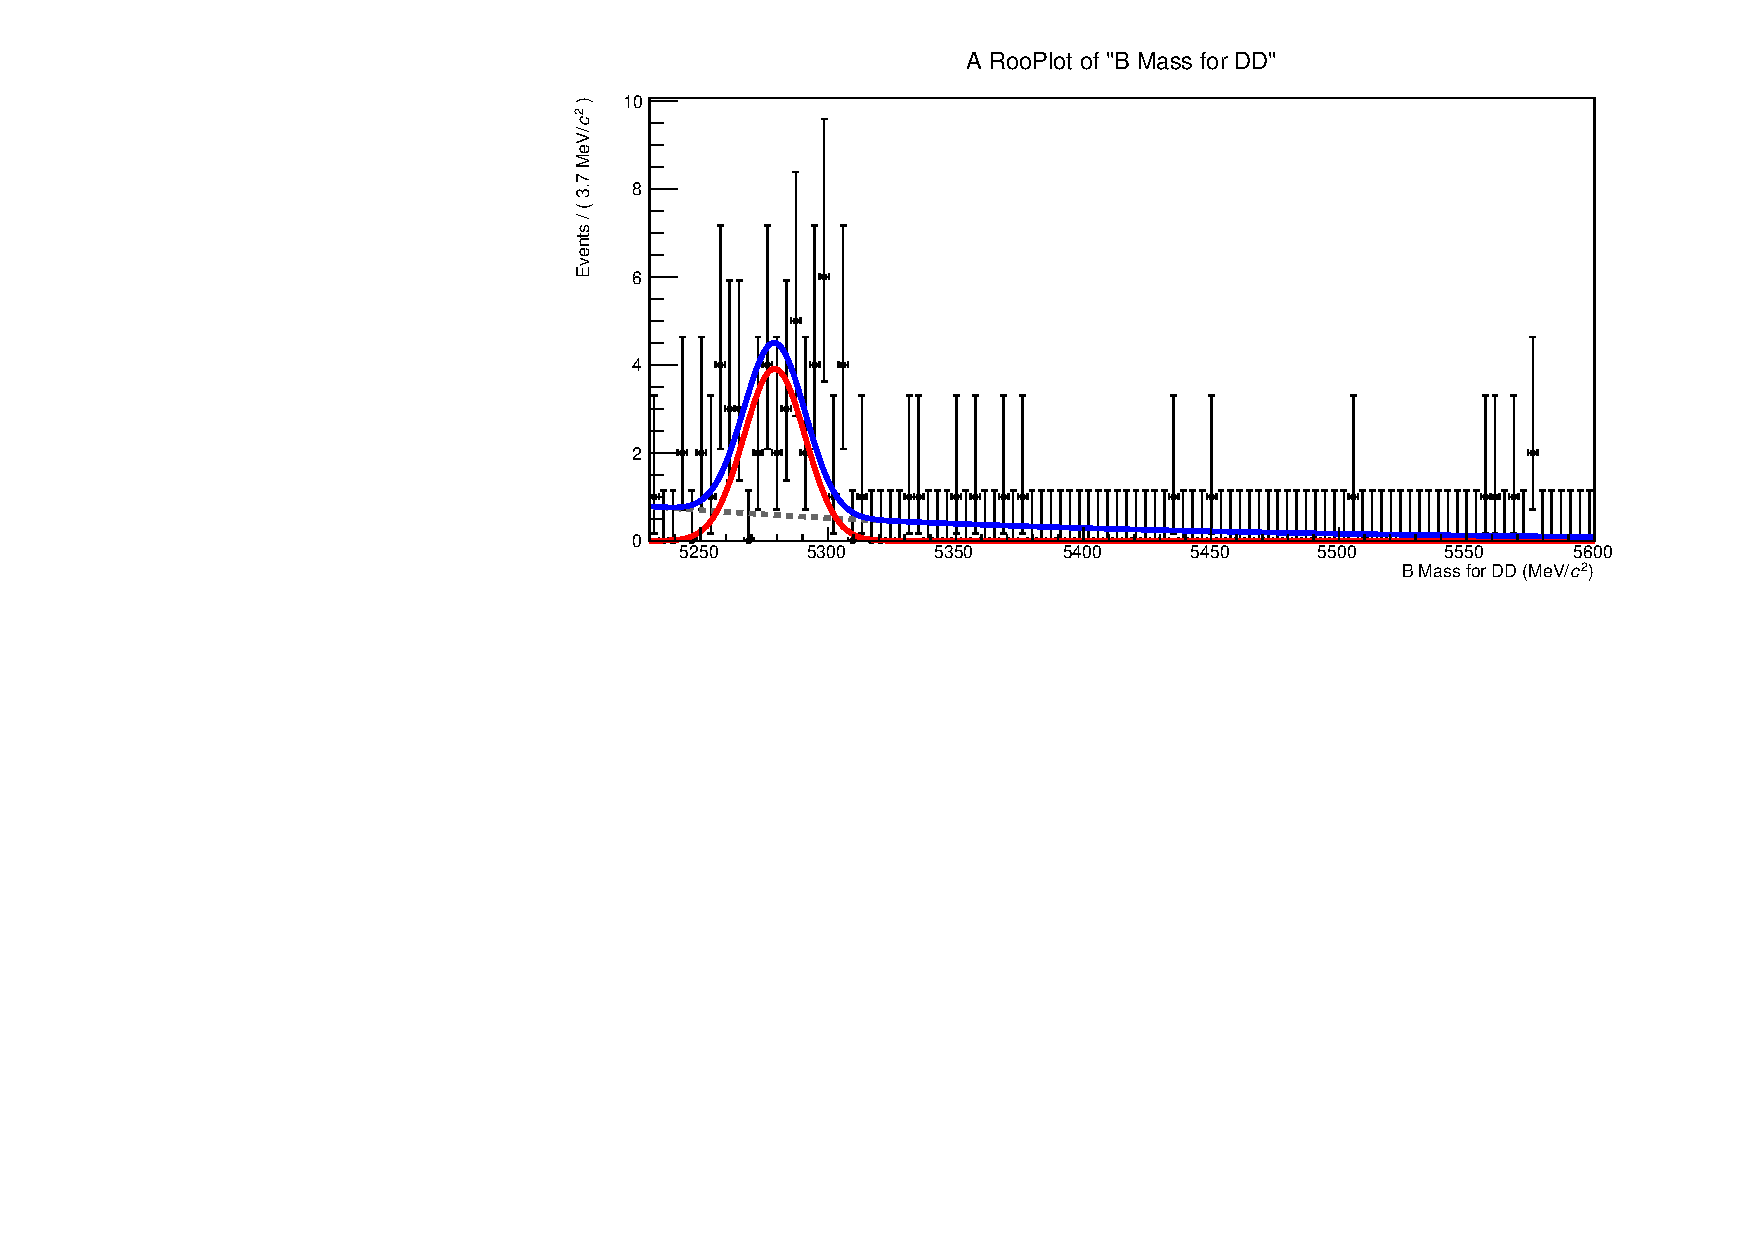
\includegraphics[width=0.7\linewidth]{figures/backgrounds/charmlessFit_PiPi_DD_FD0.pdf}
\put(-100,100) {(a)}
\hfill
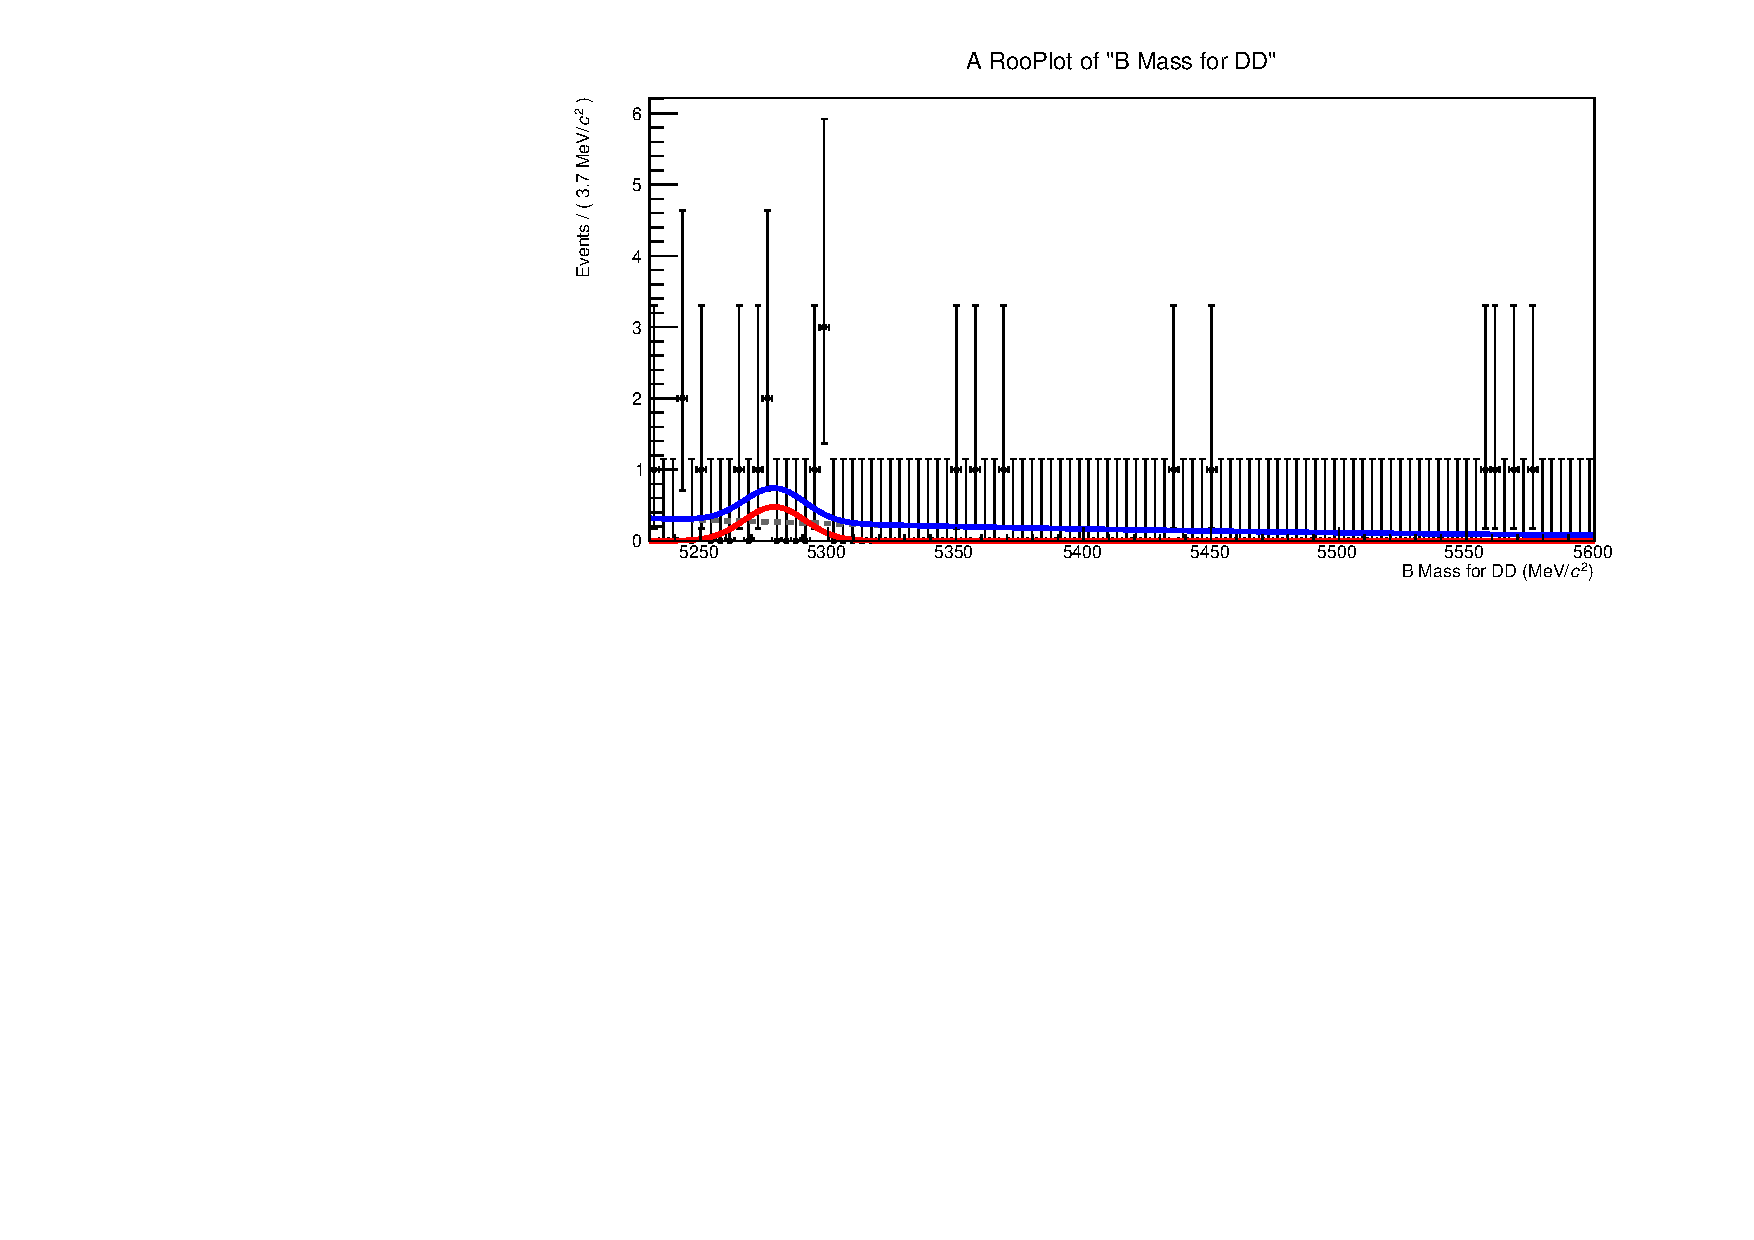
\includegraphics[width=0.7\linewidth]{figures/backgrounds/charmlessFit_PiPi_DD_FD2.pdf}
\put(-100,100) {(b)}
\caption{Fits to the Run 1 refitted B mass taking \decay{\Dz}{\pi\pi} candidates from the D mass sidebands after a FD significance cut (a) greater than 0 and (b) greater than 2$\sigma$. A Gaussian is used to model the signal and an exponential for the combinatoric background.}
\label{charmlesspipi}
\end{figure}

The yield of the \B mass peak is measured in the \D mass sidebands and then scaled to the \D mass window. This gives an estimate of the charmless yields expected after selection in the mass fit. These fits are performed using Run 1 data both with a FD significance cut of zero and a 2$\sigma$ FD cut applied, the resulting yields estimates are shown in Tables \ref{charmlessyieldsnofd} and \ref{charmlessyields} respectively. The same fits were peformed on Run 2 data and the results for the estimated charmless contribution in Run 2 for a zero and 2$\sigma$ FD cut, these are given in Tables \ref{charmlessyieldsnofdRun2} and \ref{charmlessyieldsRun2}.

\begin{table}[h] 
\centering 
\begin{tabular}{lll} 
\hline 
Mode & LL & DD \\ 
\hline 
$K\pi$ & $2.8 \pm 1.6$ & $2.6 \pm 1.9$ \\ 
$KK$ & $1.2 \pm 2.0$ & $0.6 \pm 2.2$ \\ 
$\pi\pi$ & $4.1 \pm 2.5$ & $16 \pm 4$ \\ 
$\pi K$ & $2.0 \pm 1.3$ & $0.0 \pm 0.6$ \\ 
$K\pi\pi\pi$ & $1.4 \pm 1.2$ & $1.5 \pm 2.0$ \\ 
$\pi\pi\pi\pi$ & $2.2 \pm 2.4$ & $6.8 \pm 3.5$ \\ 
$\pi K \pi\pi$ & $1.1 \pm 0.9$ & $1.3 \pm 1.2$ \\ 
\hline 
\end{tabular}
\caption{Estimated charmless contribution in Run 1 data for each of the D decay modes with a FD significance cut of zero applied} 
\label{charmlessyieldsnofd} 
\end{table}

\begin{table}[h]
\centering
\begin{tabular}{lll} 
\hline 
Mode & LL & DD \\ 
\hline 
$K\pi$ & $1.7 \pm 1.0$ & $0.2 \pm 1.6$ \\ 
$KK$ & $0.0 \pm 0.4$ & $0.0 \pm 0.4$ \\ 
$\pi\pi$ & $1.2 \pm 1.5$ & $2.0 \pm 1.6$ \\ 
$\pi K$ & $1.0 \pm 0.9$ & $0.0 \pm 0.3$ \\ 
$K\pi\pi\pi$ & $1.3 \pm 1.1$ & $0.1 \pm 3.7$ \\ 
$\pi\pi\pi\pi$ & $0.0 \pm 7.4$ & $0.0 \pm 1.2$ \\ 
$\pi K \pi\pi$ & $0.9 \pm 0.7$ & $0.0 \pm 0.7$ \\ 
\hline 
\end{tabular}
\caption{Estimated charmless contribution in Run 1 data for each of the D decay modes with a FD significance cut of 2$\sigma$ applied}
\label{charmlessyields}
\end{table}

\begin{table}[h] 
\centering 
\begin{tabular}{lll} 
\hline 
Mode & LL & DD \\ 
\hline 
$K\pi$ & $0.0 \pm 0.4$ & $0.0 \pm 1.6$ \\ 
$KK$ & $5.2 \pm 2.6$ & $7.1 \pm 4.0$ \\ 
$\pi\pi$ & $11 \pm 4$ & $30 \pm 5$ \\ 
$\pi K$ & $0.2 \pm 2.8$ & $1.1 \pm 1.7$ \\ 
$K\pi\pi\pi$ & $0.3 \pm 2.7$ & $1.6 \pm 3.3$ \\ 
$\pi\pi\pi\pi$ & $7.0 \pm 3.4$ & $8.7 \pm 5.3$ \\ 
$\pi K \pi\pi$ & $0.0 \pm 2.3$ & $0 \pm 17$ \\ 
\hline 
\end{tabular} 
\caption{Estimated charmless contribution in Run 2 data for each of the D decay modes with a FD significance cut of zero applied} 
\label{charmlessyieldsnofdRun2} 
\end{table}

\begin{table}[h] 
\centering 
\begin{tabular}{lll} 
\hline 
Mode & LL & DD \\ 
\hline 
$K\pi$ & $0.0 \pm 0.3$ & $0.6 \pm 1.3$ \\ 
$KK$ & $0.0 \pm 0.3$ & $0.0 \pm 0.7$ \\ 
$\pi\pi$ & $0.0 \pm 1.2$ & $2.3 \pm 2.2$ \\ 
$\pi K$ & $0.4 \pm 1.0$ & $0.0 \pm 0.5$ \\ 
$K\pi\pi\pi$ & $1.0 \pm 1.4$ & $0.0 \pm 7.6$ \\ 
$\pi\pi\pi\pi$ & $1.4 \pm 2.3$ & $0.0 \pm 1.0$ \\ 
$\pi K \pi\pi$ & $0.0 \pm 10.6$ & $1.4 \pm 1.5$ \\ 
\hline 
\end{tabular} 
\caption{Estimated charmless contribution in Run 2 data for each of the D decay modes with a FD significance cut of 2$\sigma$ applied} 
\label{charmlessyieldsRun2}
\end{table}

The \Dz FD significance is required to exceed 2$\sigma$, therefore from Tables \ref{charmlessyields} and \ref{charmlessyieldsRun2} it can be seen that all charmless contributions are consistent with zero. The expected yields in the $K\pi$ favoured and $KK$ modes are significantly less than 1\% of the expected signal yield. However, the charmless contribution in the $\pi\pi$ mode could be significant. A systematic is assigned to the possible charmless contribution in the $\pi\pi$ mode, details are given in Section \ref{sec:systematics}. 

\subsubsection{\decay{\B}{\D\pi\pi\pi}}
\label{sec:backgrounds:b2dpipipi}

\decay{\B}{\D\pi\pi\pi} decays, with a branching fraction of $5.7 \times 10^{-3}$~\cite{PDG2014} (about 50 times the signal branching fraction), are expected to occur as a peaking background underneath the signal. In order to remove this background, events are selected with the requirement that the \KS has flown. For DD candidates this requirement is already satisfied, however for LL candidates the flight distance significance of the \KS in the z direction, with the equivalent definition as for \Dz given in Equation \ref{FDdefinition}, is required to exceed 5$\sigma$. 

The \decay{\B}{\D\pi\pi\pi} background is removed by taking the \KS mass sidebands ($>$ 20 MeV from nominal \KS mass) in data and performing a fit to the invariant \B mass distribution. All DTF variables are replaced in the selection as descibed in Section \ref{sec:backgrounds:charmless}. This fit to data is performed for the favoured \decay{\Dz}{\Km\pip} mode with a FD significance cut of both zero and 5$\sigma$, as shown in Figure \ref{strangelessfits}. It can be seen that the 5$\sigma$ FD significance selection removes all of the \decay{\B}{\D\pi\pi\pi} background.

\begin{figure}
\centering
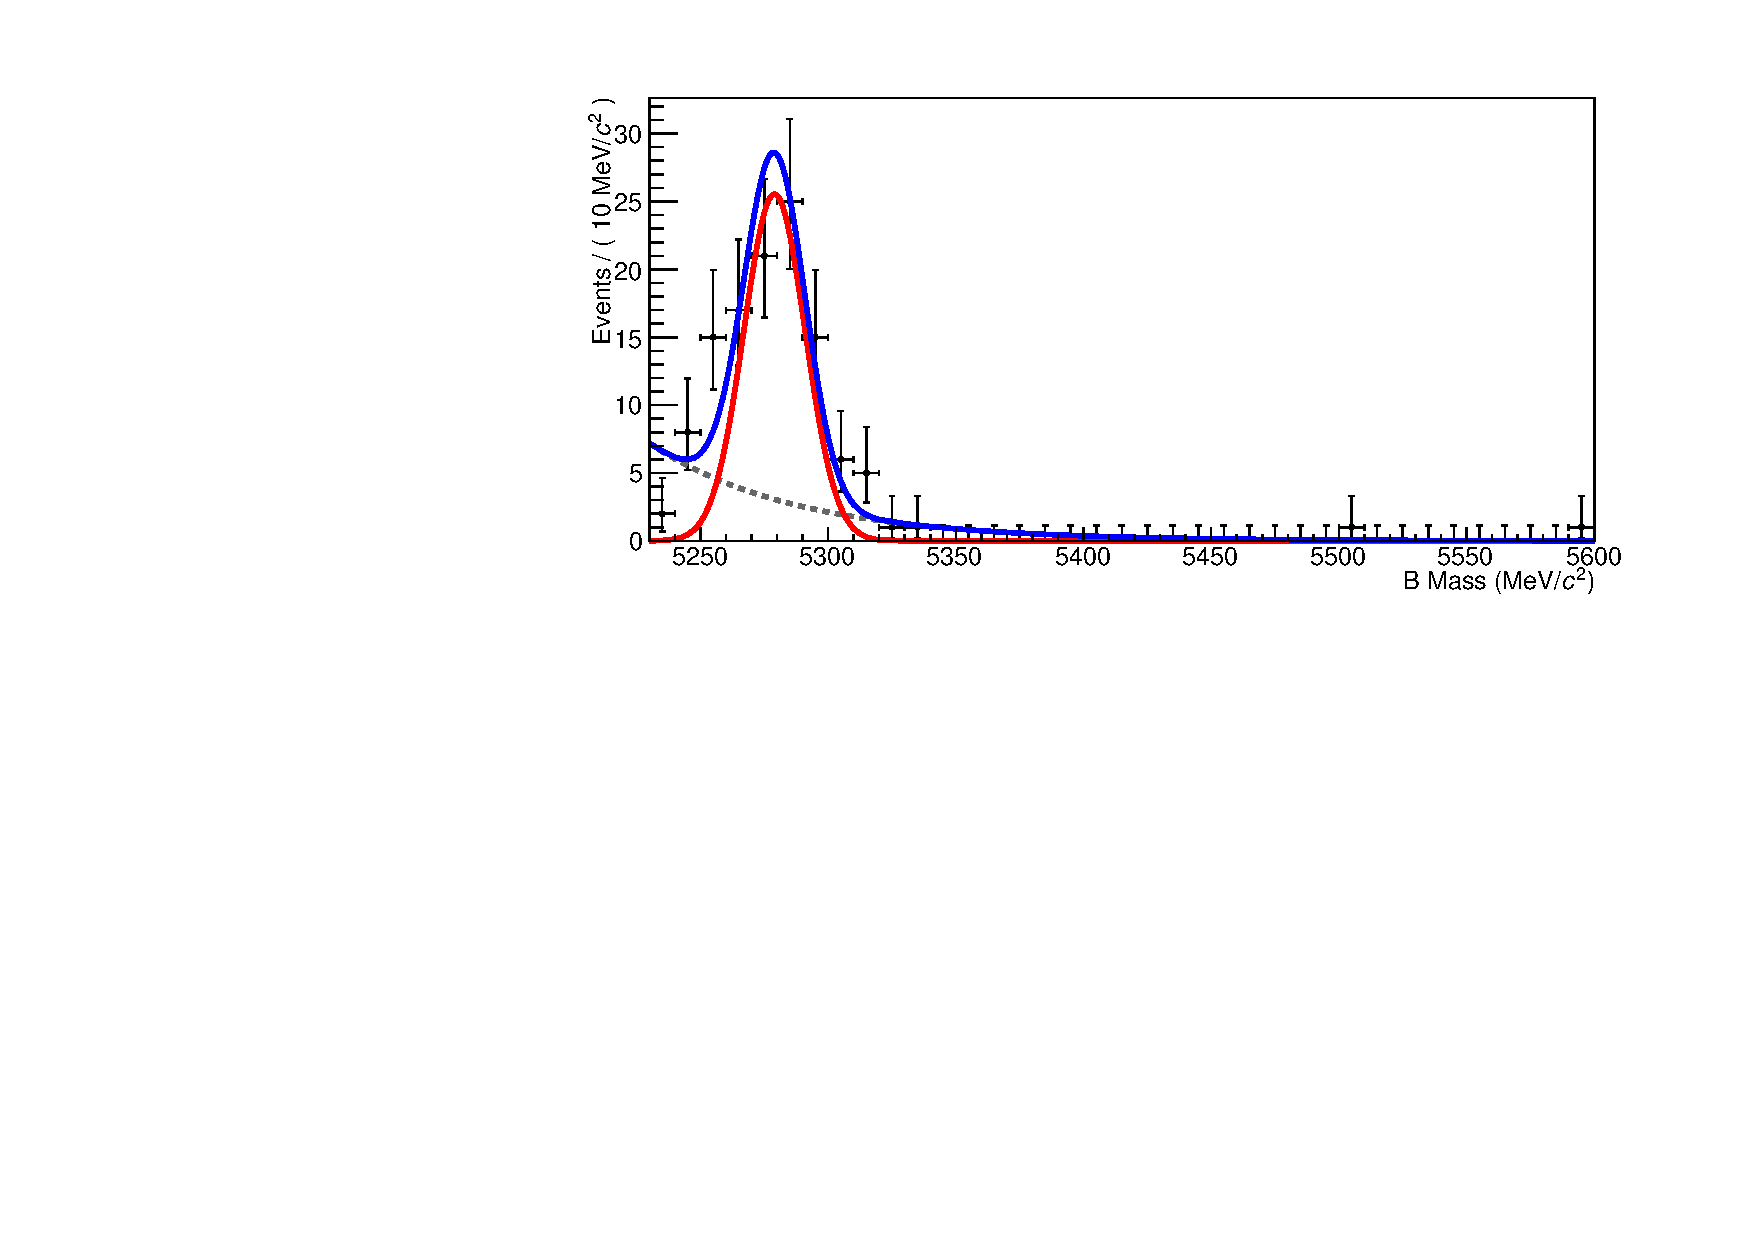
\includegraphics[width=0.7\linewidth]{figures/backgrounds/B2DpipipiFit_KPi_LL_FD0_run2.pdf}
\put(-100,100) {(a)}
\hfill
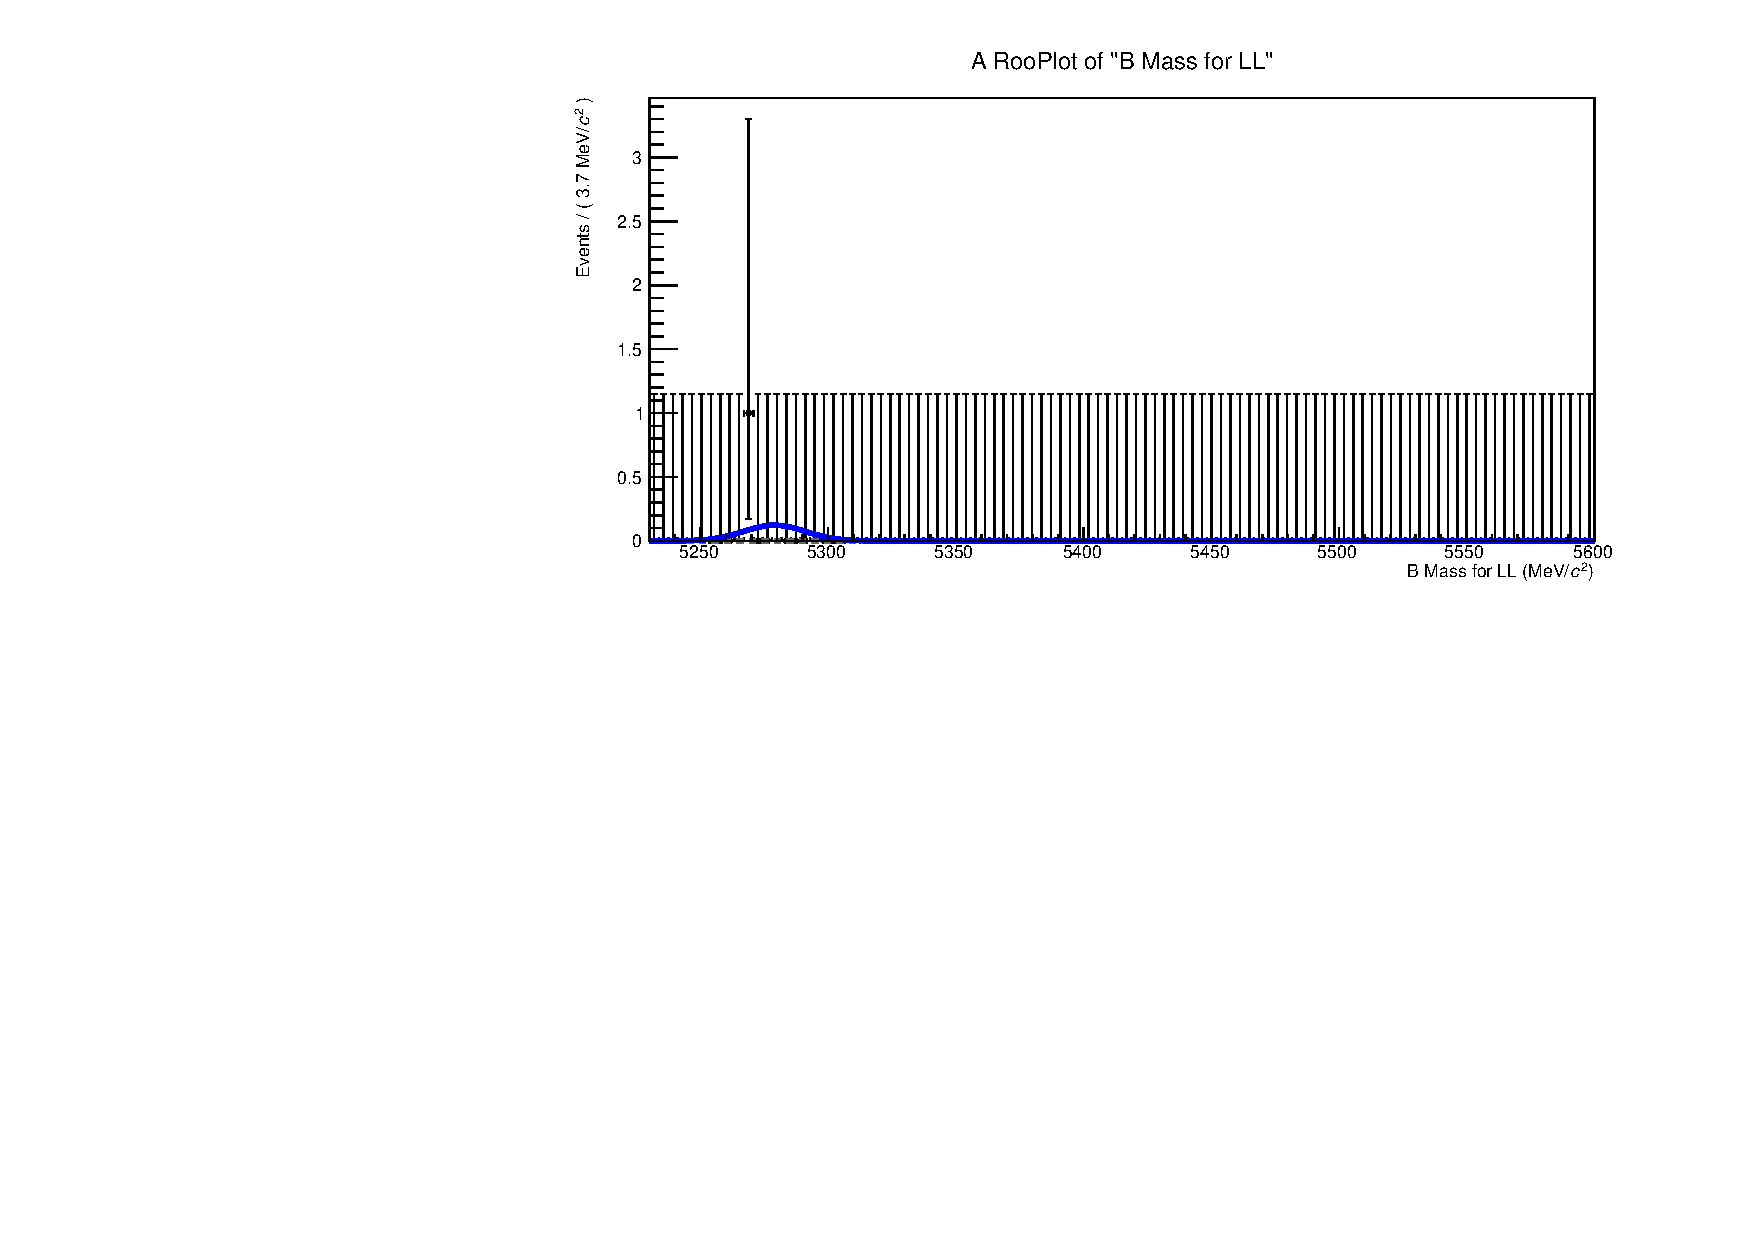
\includegraphics[width=0.7\linewidth]{figures/backgrounds/B2DpipipiFit_KPi_LL_FD5_run2.pdf}
\put(-100,100) {(b)}
\caption{Fits to the Run 2 refitted B mass taking \decay{\Dz}{\Km\pip} candidates from the \KS mass sidebands after a FD significance cut (a) greater than 0 and (b) greater than 5$\sigma$. Expected  \decay{\B}{\D\pi\pi\pi} yield in the signal region with FD significance $>$ 0 is $77 \pm 11$ and signal yield with FD significance $>$ 5 is $1.0 \pm 1.0$. A Gaussian is used to model the signal and an exponential for the combinatoric background}
\label{strangelessfits}
\end{figure}

\subsubsection{Non-resonant $B \to DK_s\pi$}
\label{sec:backgrounds:non-resonant}

Non-resonant background is reduced by removing events in which the \KS\pion invariant mass is greater than 75 MeV from the nominal \Kstarpm mass. \decay{\Bpm}{\D\Kstarpm} is a Scalar $\to$ Scalar Vector decay, which means the \Kstarpm must be londitudially polarised, so the $K_s$ helicity angle of pure \D\Kstarpm events follows a $\cos^2\theta$ distribution, as shown in Figure \ref{helicitycut}, compared to the uniform distribution of non-resonant components. It can be seen from Figure \ref{helicitycut} that the \KS helicity angle distribution is not symmetric, this is discussed in detail in Appendix \ref{sec:app:helicityangle}. Removing events with an absolute value of $\cos^2\theta$ less than 0.3 improves the purity of \D\Kstarpm decays compared to non-resonant background.

\begin{figure}[h]
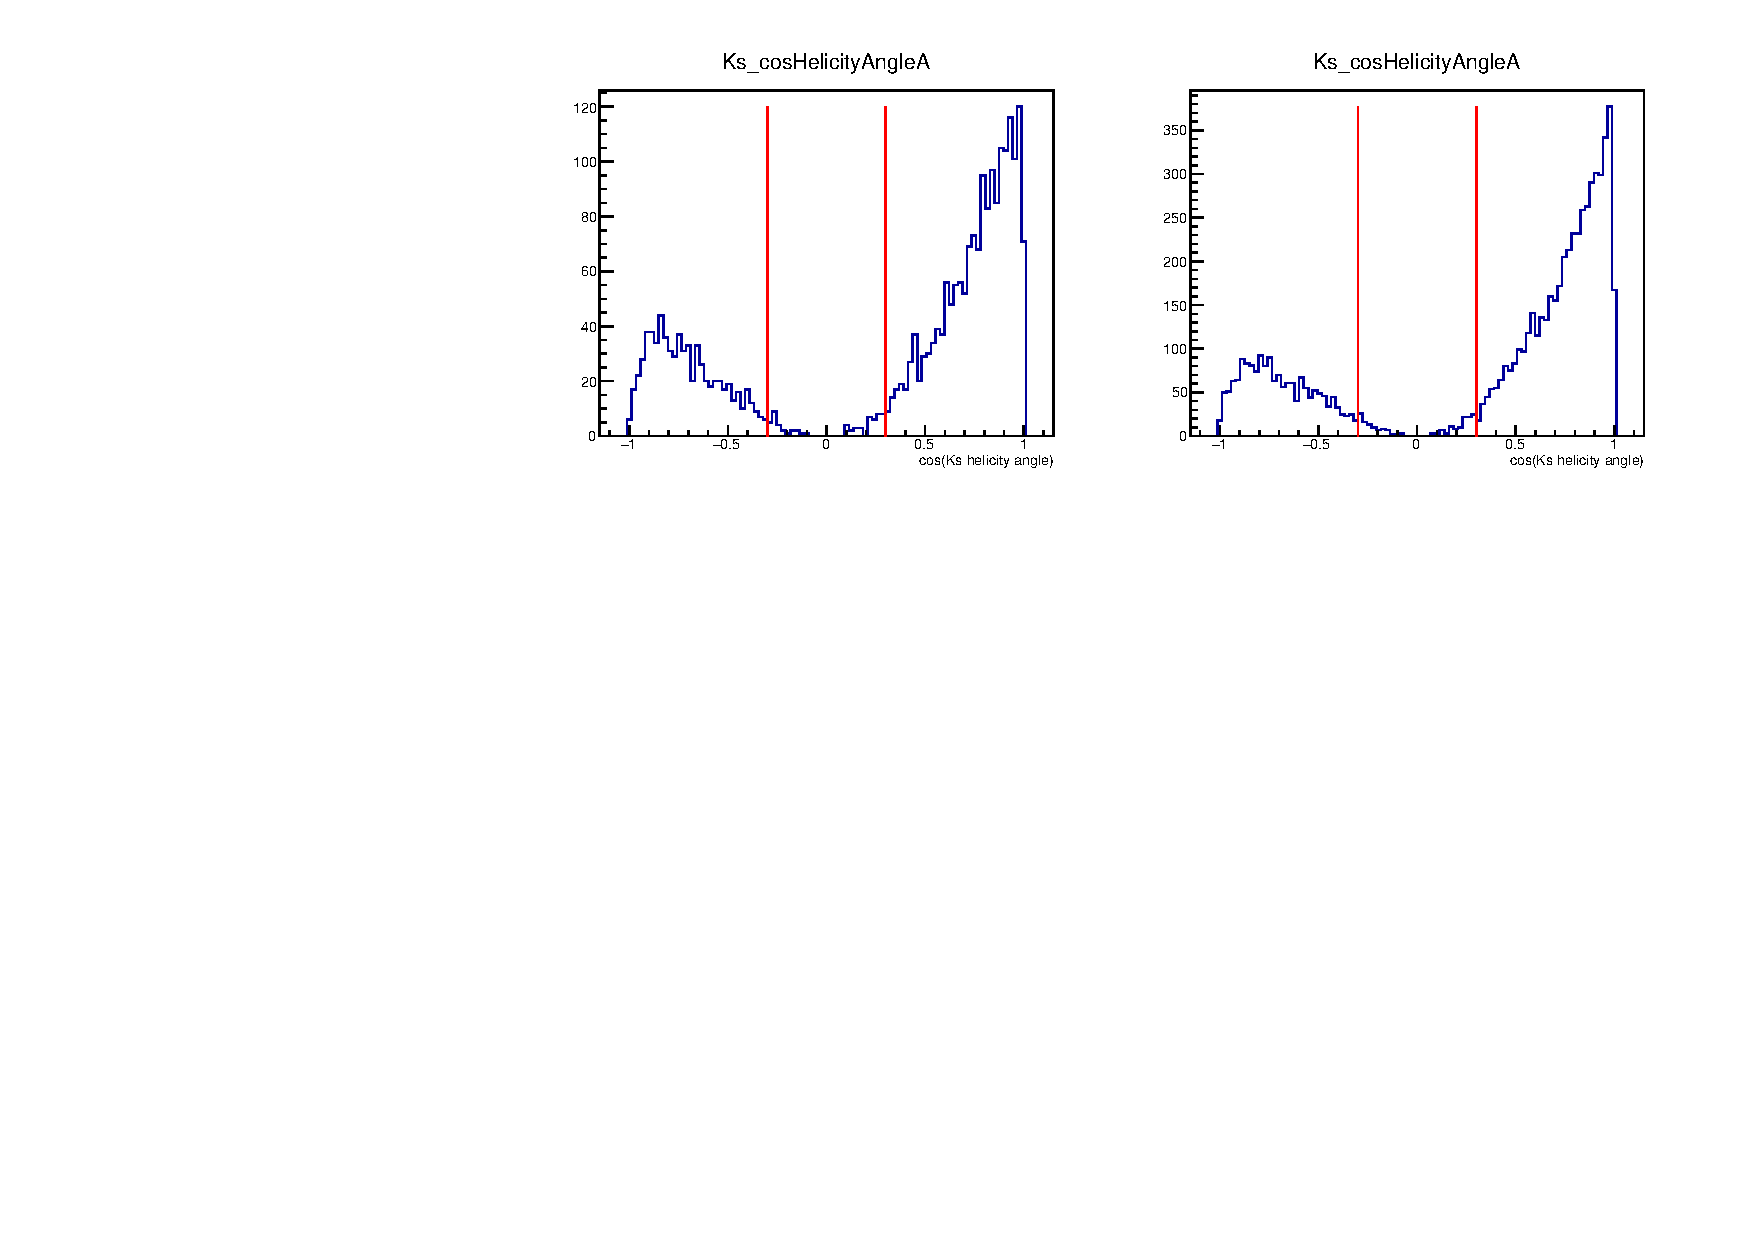
\includegraphics[width=\linewidth]{figures/backgrounds/KsHelicityCut.pdf}
\put(-400,100) {(a)}
\put(-170,100) {(b)}
\caption{MC distribution of the cosine of Ks helicity angle for (a) LL candidates and (b) DD candidates}
\label{helicitycut}
\end{figure}

It is necessary to estimate the fraction of non-resonant \decay{\B}{\D\KS\pi} in the signal candidates. Figure \ref{kshelicitycomparison} shows a comparison of \KS helicity angle and the \KS momentum between signal MC and sWeighted data. There is a discrepancy in both \KS helicity angle distribution and the \KS momentum distribution. The discrepancy in the momentum distribution was corrrected by reweighting the MC, the resulting helicity angle distribution is consistent with the data, as shown in Figure \ref{kshelicitycomparisonreweighted}.

\begin{figure}[h]
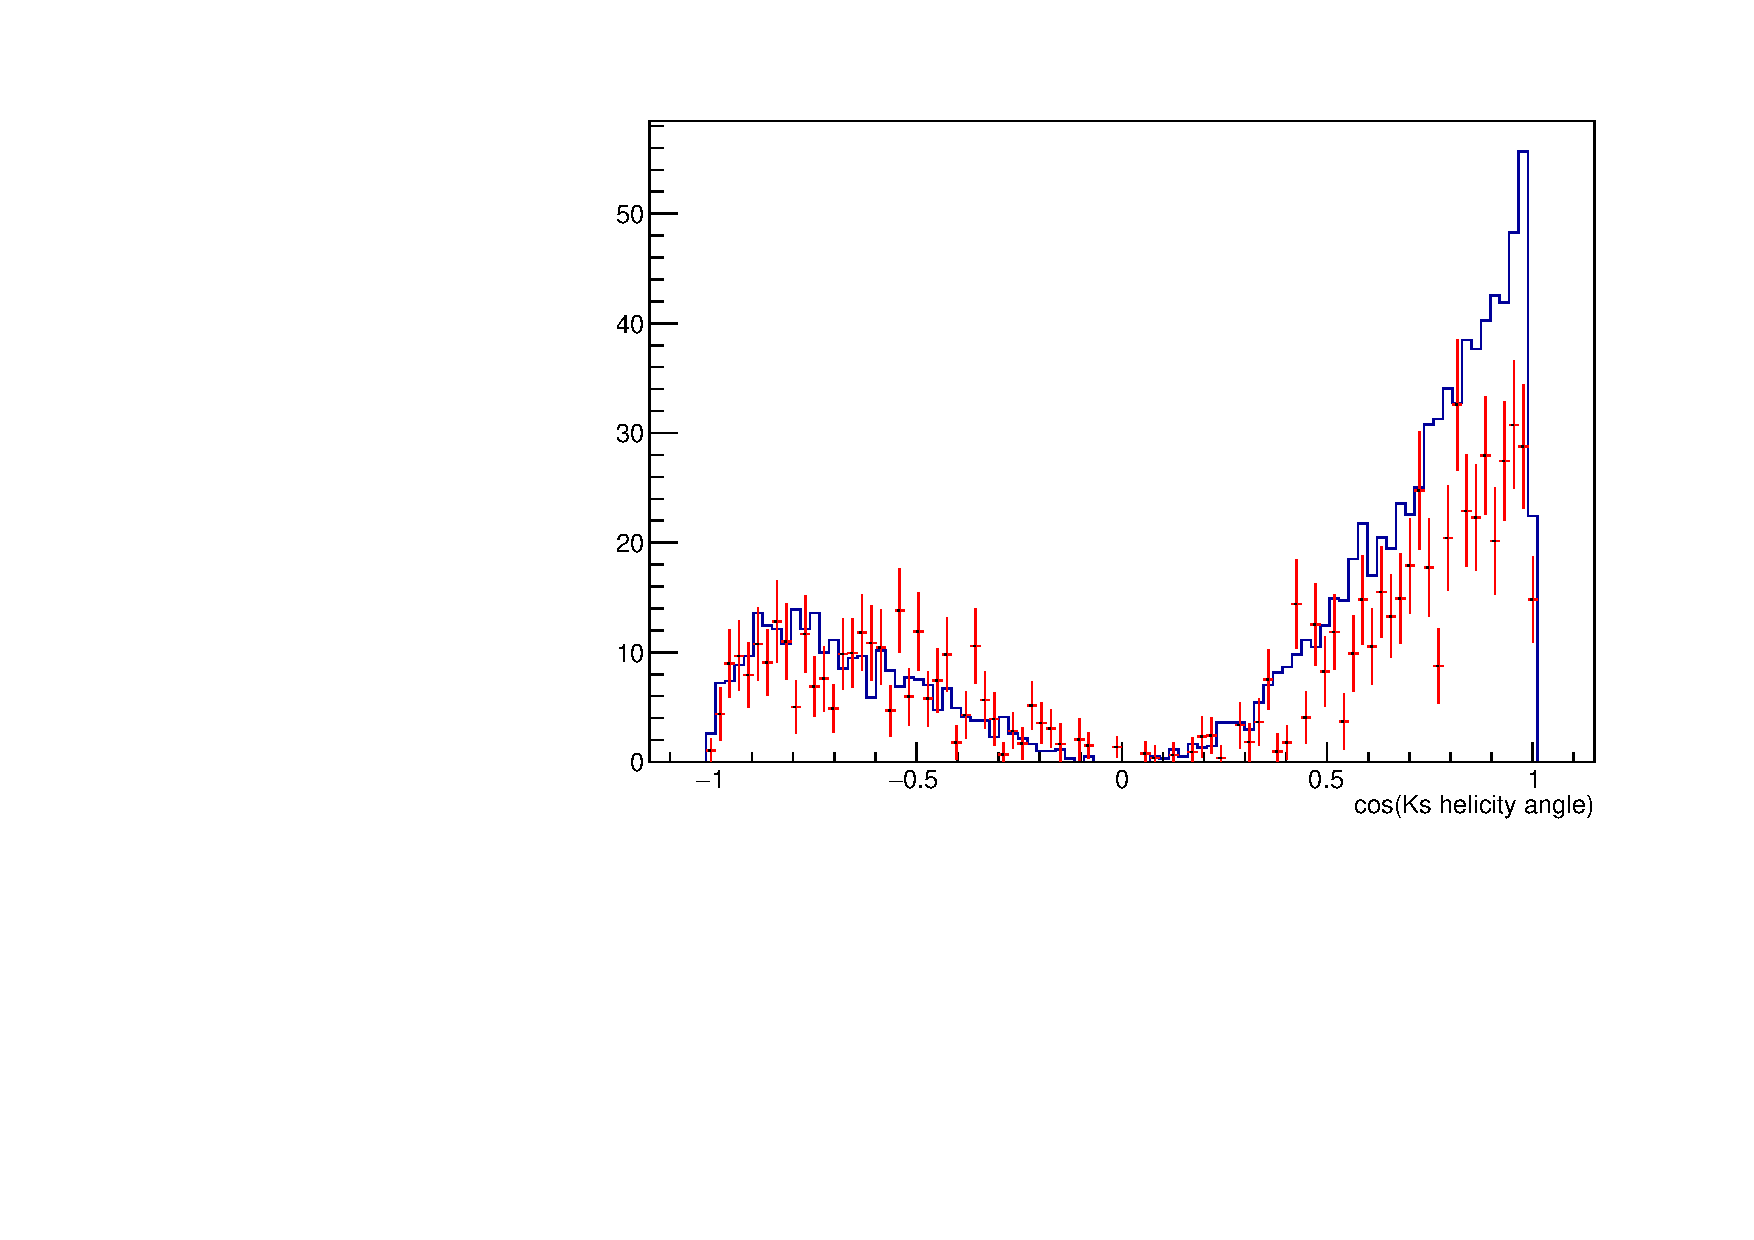
\includegraphics[width=0.5\linewidth]{figures/backgrounds/KsHelicityAngle_sweighted.pdf}
\put(-170,100) {(a)}
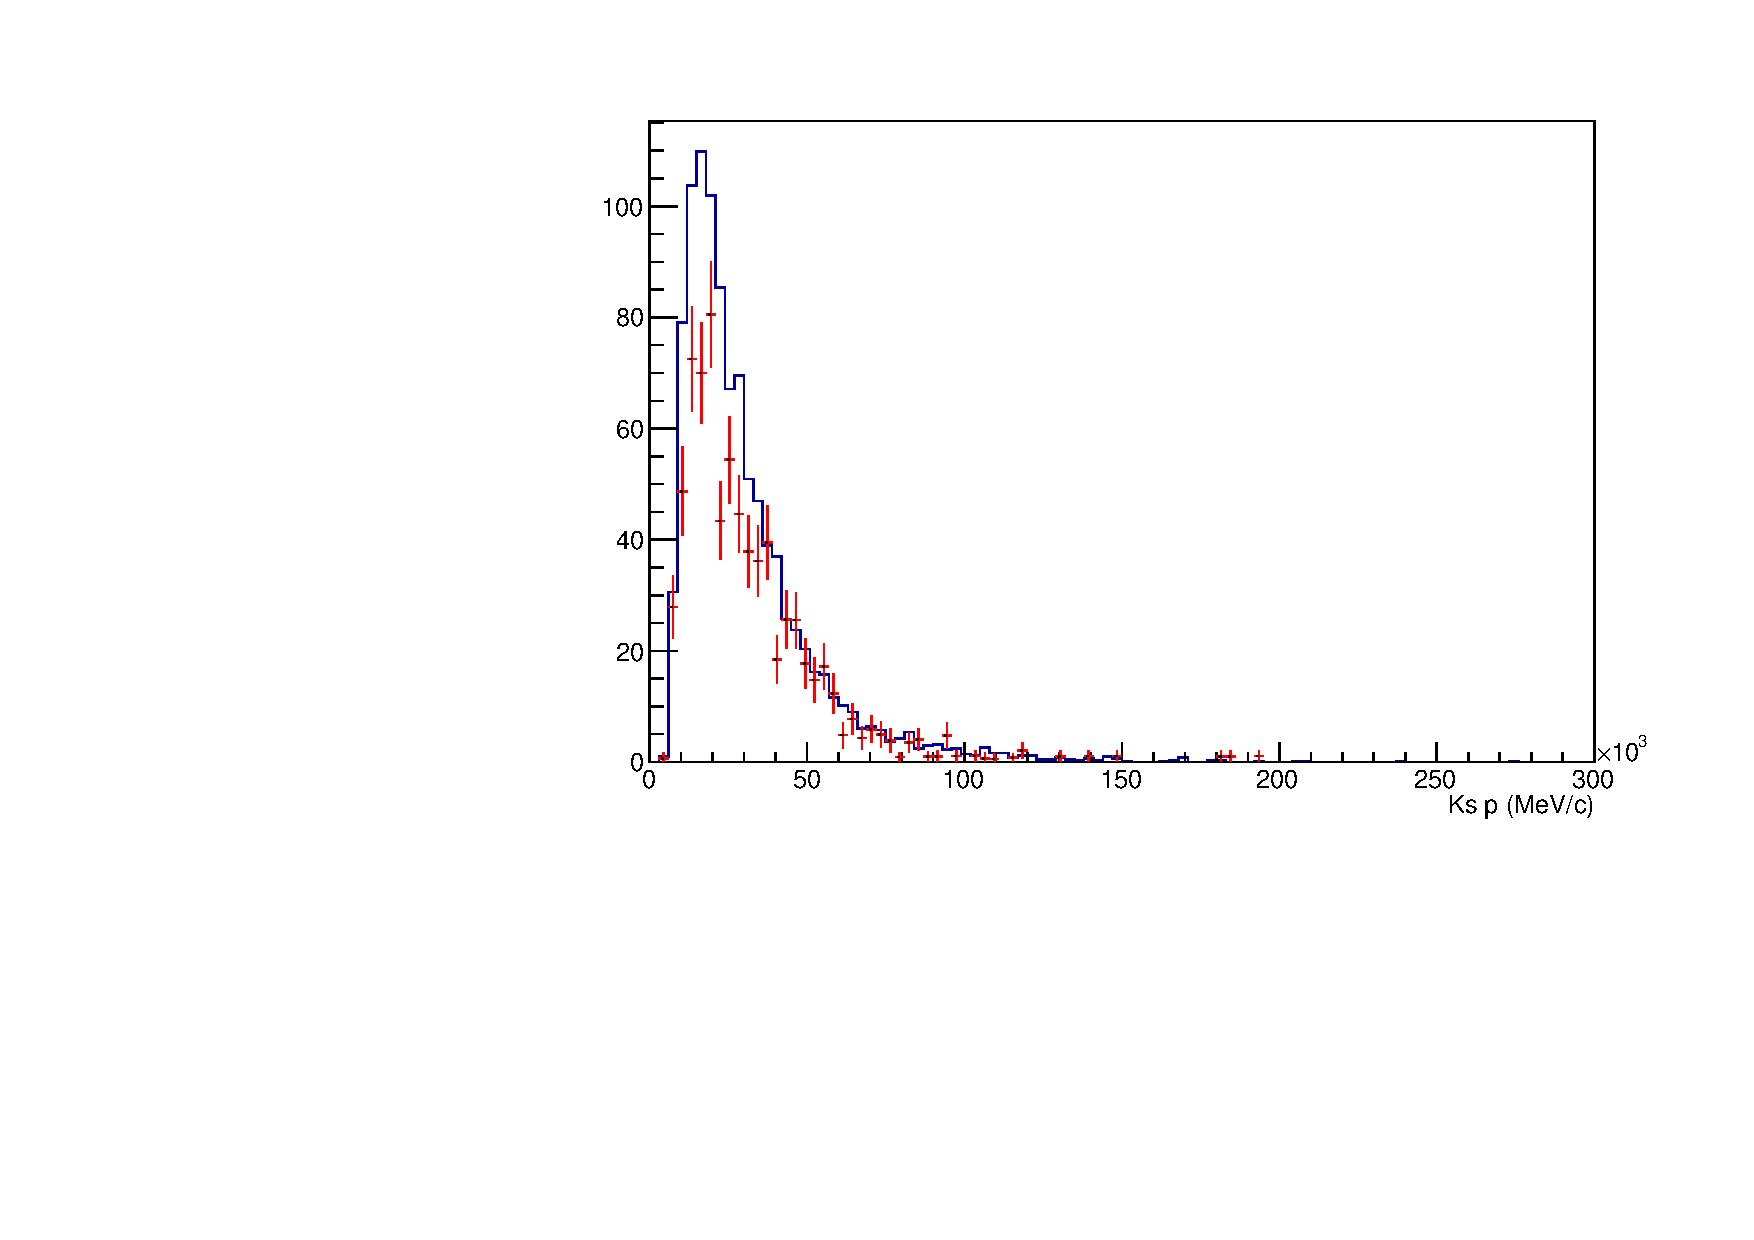
\includegraphics[width=0.5\linewidth]{figures/backgrounds/KsP_sweighted.pdf}
\put(-170,100) {(b)}
\caption{Comparison of (a) cosine of the helicity angle distribution and (b) the \KS momentum distribution in sWeighted data (red) and MC (blue)}
\label{kshelicitycomparison}
\end{figure}

\begin{figure}[h]
\centering
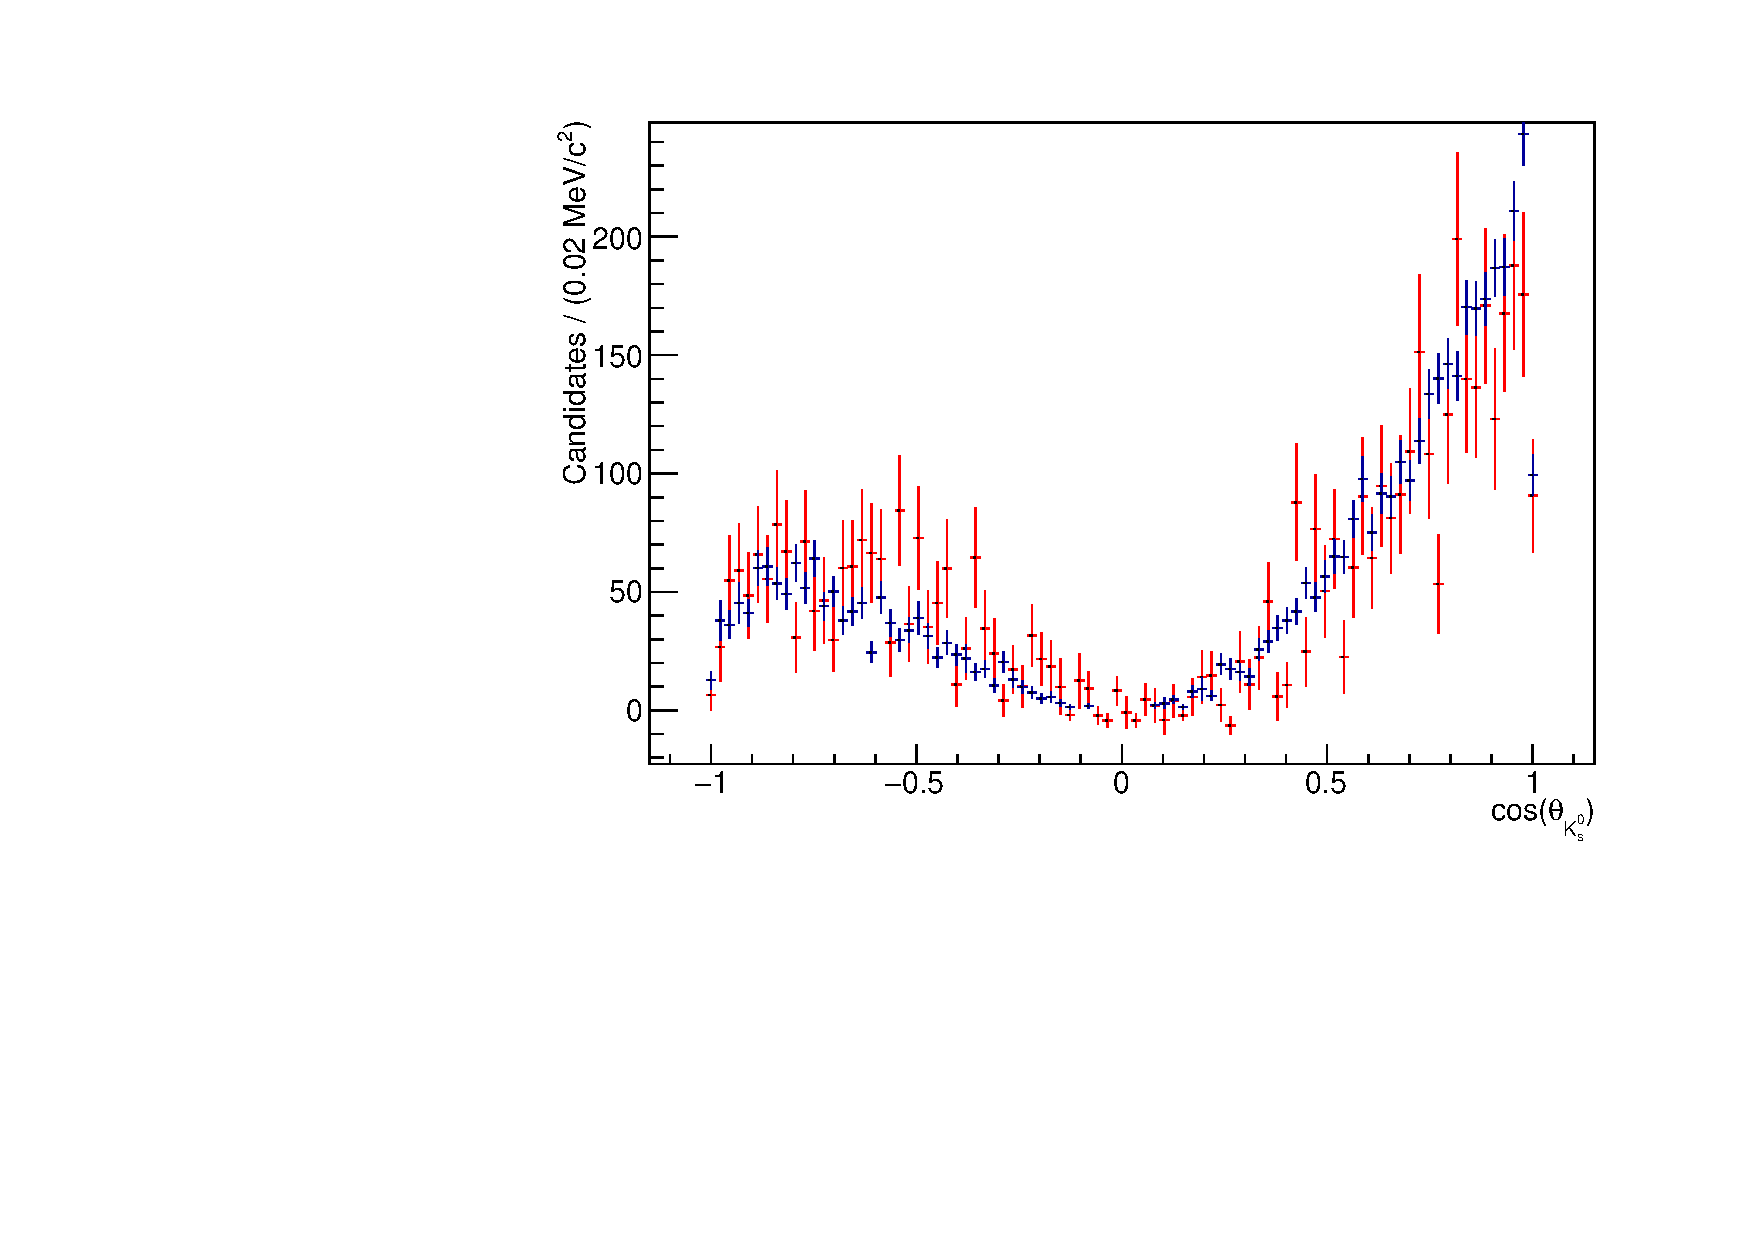
\includegraphics[width=0.6\linewidth]{figures/backgrounds/KsHelicityAngle_sweighted_MCweighted.pdf}
\caption{Comparison of cosine of the helicity angle distribution in sWeighted data (red) and MC (blue) reweighted to give the same \KS momentum distribution}
\label{kshelicitycomparisonreweighted}
\end{figure}

The parameter $\kappa$, defined in Section \ref{sec:interpretation:coherence}, is a measure of the non-$DK(892)^*$ contribution, which is expected to mainly consist of non-resonant contribution, but could include other resonances. In this analysis the value of $\kappa$ is estimated and then used alongside the \CP observables to extract \Pgamma, $r_B$ and $\delta_B$. The parameter $\kappa$ is estimated by constructing an amplitude model and generating many toys by varying the amplitudes and phases of the model components, this method is detailed in Section \ref{sec:interpretation:coherence}. The estimated value of $\kappa$ is $0.95 \pm 0.06$.

\subsubsection{Favoured $\to$ Supressed crossfeed}
\label{sec:backgrounds:crossfeed}

The doubly Cabibo supressed ADS mode, \decay{\Bm}{\D(\Kp\pim)\Kstarm}, can have contamination coming from the favoured \decay{\Bm}{\D(\Km\pip)\Kstarm} mode, where the daughter mass hypotheses are swapped, i.e. the kaon is misidentified as a pion and the pion is misidentified as a kaon. The favoured mode has a braching ratio 281 times higher than the ADS mode. Implementation of PID cuts of the \D daughters significantly reduces this background, however in order to reduce it to negligible levels a veto is applied. The \Dz mass is reconstructed where both daughter mass hypotheses are swapped, this is required to be greater than 15 MeV away from the nominal \Dz mass. This veto window is illustrated in Figure \ref{Dmassveto}, which shows the MC distributions for DD canidates in Run 1. The veto is only applied to the ADS mode in this analysis. It is found to be 92.5\% efficient at retaining genuine signal, corresponding to events that lie within the red lines in Figure \ref{Dmassveto} (a), while only retaining 8.7\% of double misID background, coresponding to events that lie within the red lines in Figure \ref{Dmassveto} (b). For the 4-body modes the same background can appear in the suppressed \decay{\Bm}{\D(\Kp\pim\pip\pim)\Kstarm} mode due to contamination from the favoured \decay{\Bm}{\D(\Km\pip\pim\pip)\Kstarm}. There are two \pip mesons that could be misidetified as a \Kp meson, therefore in this case two vetos need to be applied. The \Dz mass is reconstructed as a swapped mass hypothesis where the kaon is swapped with the lower momentum pion and the kaon is swapped with the higher momentum pion. The veto is applied to both these reconstructed masses as shown in Figure \ref{Dmassveto4body}.

\begin{figure}[h]
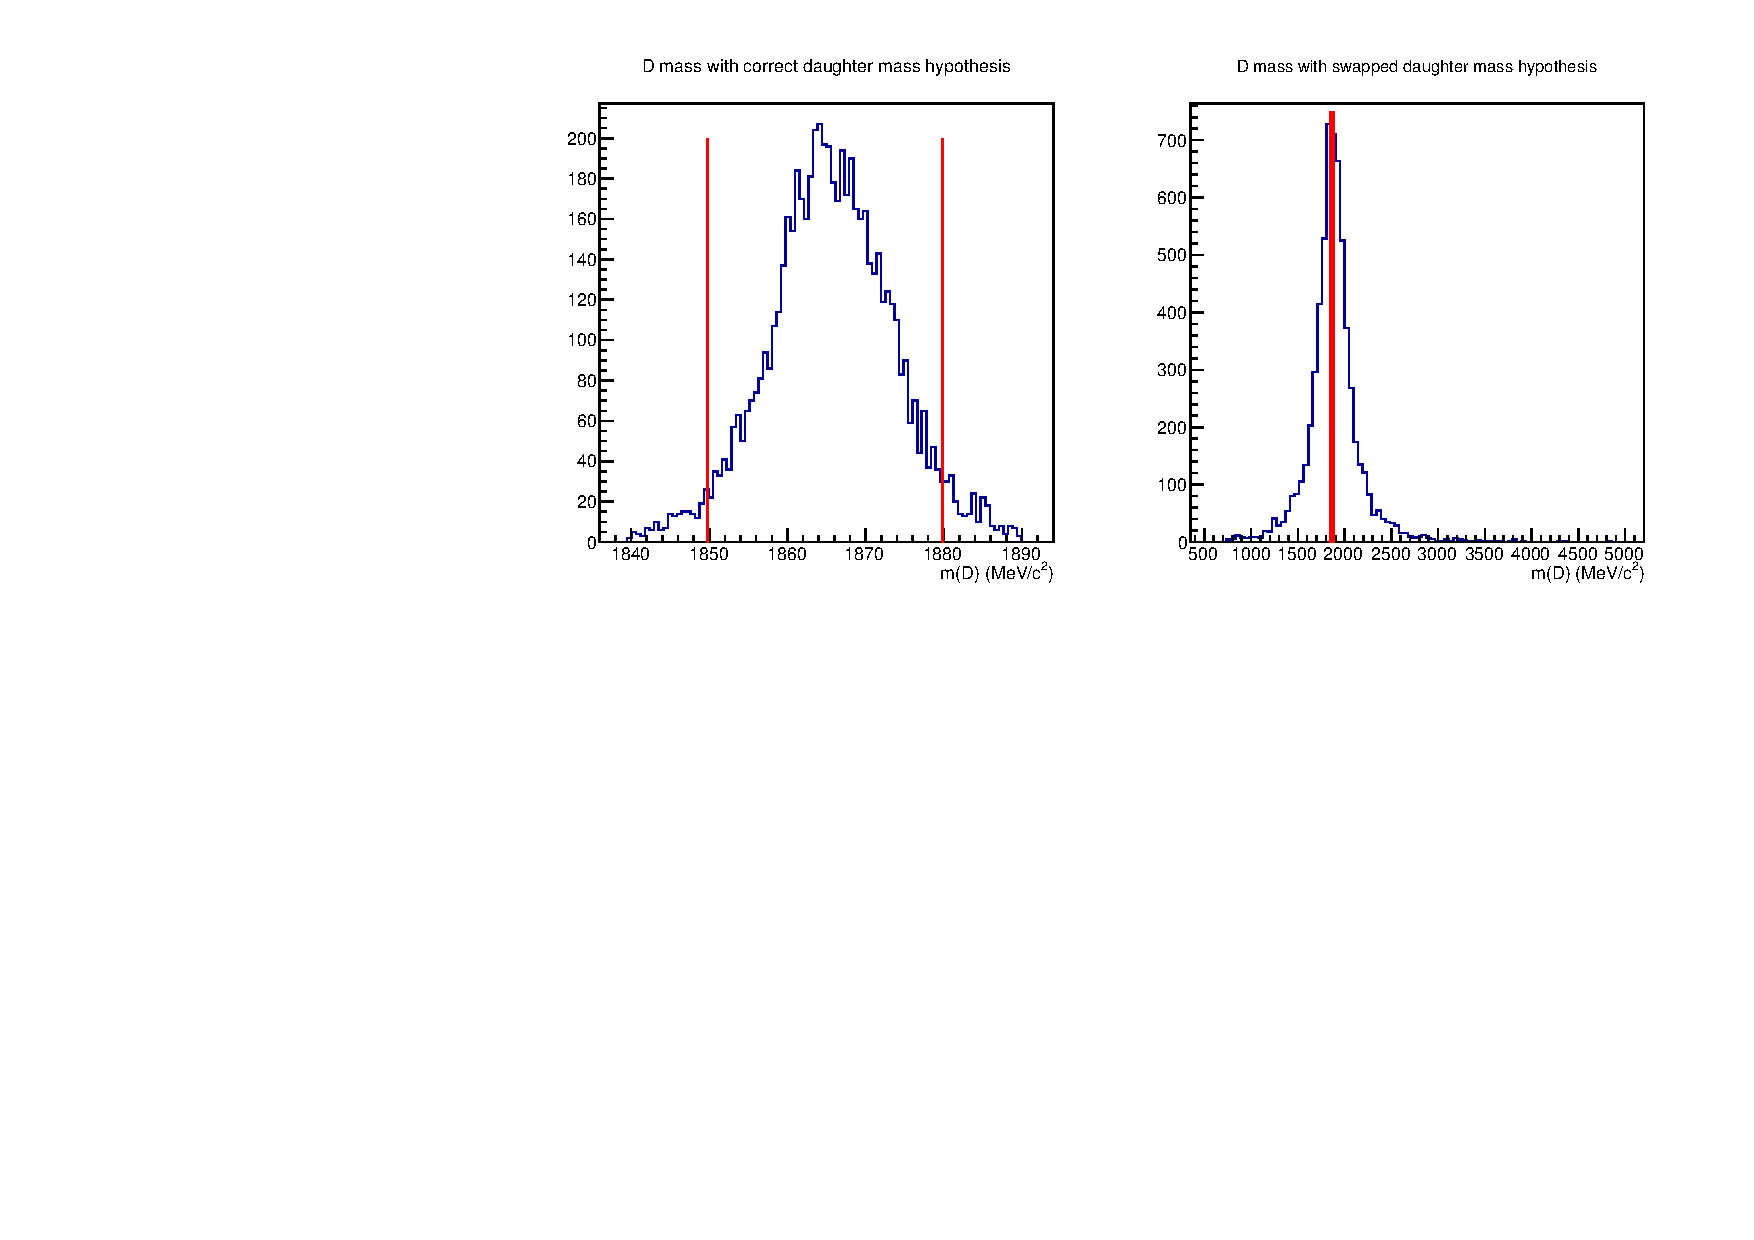
\includegraphics[width=\linewidth]{figures/backgrounds/Dmassveto.pdf}
\put(-410,150) {(a)}
\put(-180,150) {(b)}
\caption{MC distributions for DD canidates in Run 1 showing D mass with (a) the correct D daughter mass hypothesis and (b) the swapped D daughter mass hypothesis. The red lines correcpond to the double misID veto selection window applied to the ADS mode}
\label{Dmassveto}
\end{figure}

\begin{figure}[h]
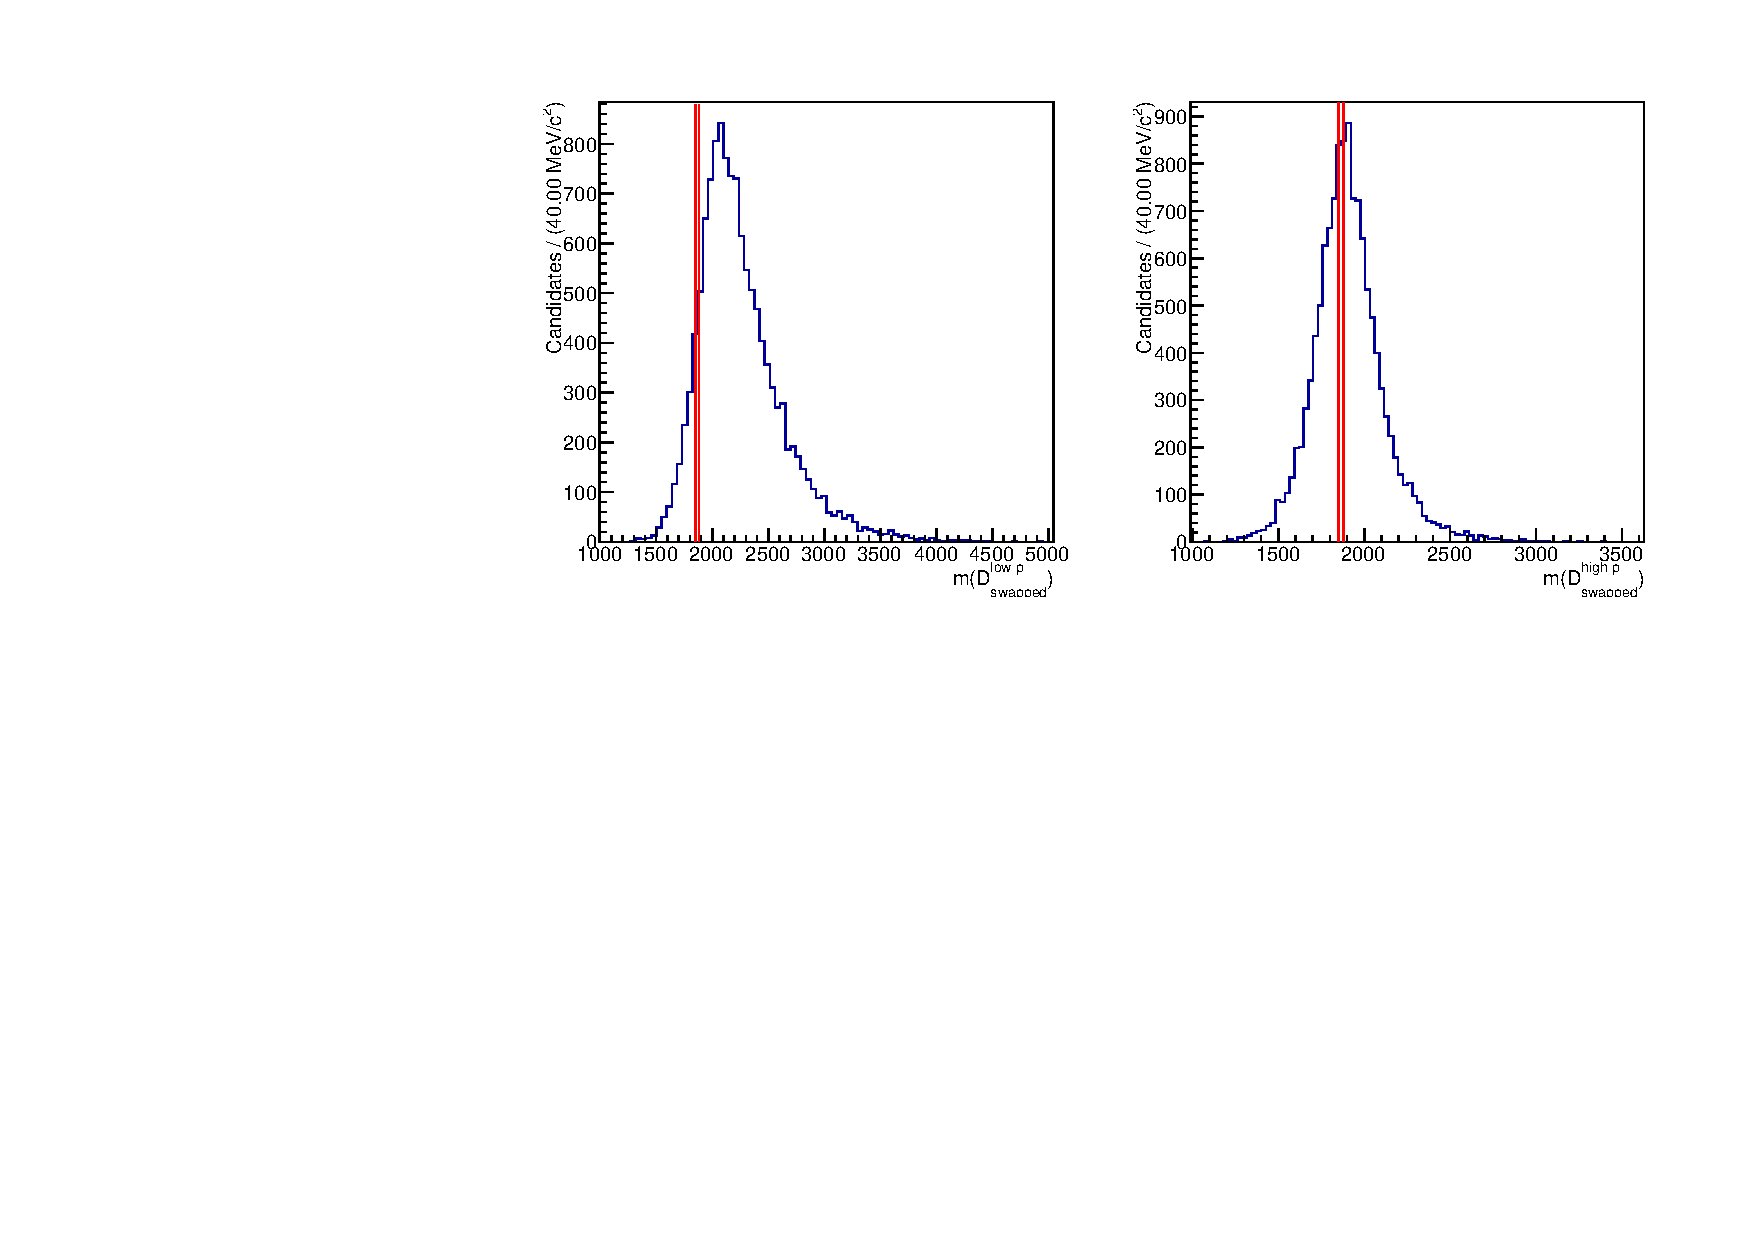
\includegraphics[width=\linewidth]{figures/backgrounds/Dmassveto_4body.pdf}
\put(-410,150) {(a)}
\put(-180,150) {(b)}
\caption{MC distributions for DD canidates in Run 2 showing the swapped D daughter mass hypothesis where (a) the kaon is swapped with the lower momentum pion and (b) the kaon is swapped with the higher momentum pion. The red lines correspond to the double misID veto selection window applied to the suppressed mode}
\label{Dmassveto4body}
\end{figure}

In order to determine the overall crossfeed contamination in the supressed mode the efficiency of the D mass window, double misID veto and PID requirements are taken into account for both the normal and swapped \Dz mass hypothesis. For the 2-body mode, these efficiencies are listed in Tables \ref{crossfeedefficienciesRun1} and \ref{crossfeedefficienciesRun2}. The proportion of events that will enter the supressed mode fit relative to the total \decay{\Bm}{\D(\Kp\pim)\Kstarm} is estimated to be $9.5 \times 10^{-3}$ for LL and $6.5 \times 10^{-3}$ for DD in Run 1, and $5.6 \times 10^{-3}$ for LL and $5.3 \times 10^{-3}$ in Run 2. Similarly for the 4-body mode, the efficiencies are listed in Tables \ref{crossfeedefficienciesk3piRun1} and \ref{crossfeedefficienciesk3piRun2}. The proportion of events that will enter the supressed mode fit relative to the total \decay{\Bm}{\D(\Kp\pim\pip\pim)\Kstarm} is estimated to be $2.7 \times 10^{-3}$ for LL and $1.0 \times 10^{-3}$ for DD in Run 1, and $1.4 \times 10^{-3}$ for LL and $6.3 \times 10^{-4}$ in Run 2. Therefore, the contribtuion of the crossfeed in the supressed mode is negligible.

%The tighter BDT cut applied in the ADS mode for DD candidates also has to be taken into account. The relative BDT efficiency is 0.877 for Run 1 and 0.902 for Run 2.

\begin{table}[h]
\centering
\begin{tabular}{ccc}
\hline
Selection cut & $[K_K^-\pi_\pi^+]_D$ efficiency & $[K_\pi^-\pi_K^+]_D$ efficiency \\
\hline
\Dz window: $\pm$ 25 MeV & 0.961 $\pm$ 0.003 & 0.116 $\pm$ 0.005 \\
Crossfeed veto $\pm$ 15 MeV & 0.930 $\pm$ 0.004 & 0.122 $\pm$ 0.014 \\
PID selection & 0.734 $\pm$ 0.002 & 0.00158 $\pm$ 0.00002 \\
\hline
Total & 0.655 $\pm$ 0.004 & (2.2 $\pm$ 0.3) $\times 10^{-5}$ \\
\hline
\end{tabular}
\begin{tabular}{ccc}
\hline
Selection cut & $[K_K^-\pi_\pi^+]_D$ efficiency & $[K_\pi^-\pi_K^+]_D$ efficiency \\
\hline
\Dz window: $\pm$ 25 MeV & 0.961 $\pm$ 0.002 & 0.123 $\pm$ 0.003 \\
Crossfeed veto $\pm$ 15 MeV & 0.925 $\pm$ 0.002 & 0.087 $\pm$ 0.007 \\
PID selection & 0.747 $\pm$ 0.002 & 0.00144 $\pm$ 0.00005 \\
\hline
Total & 0.663 $\pm$ 0.003 & (1.53 $\pm$ 0.14) $\times 10^{-5}$ \\
\hline
\end{tabular}
\caption{Efficiencies of the \Dz mass window, crossfeed veto and \Dz daughter PID cuts for \decay{\Bpm}{[\Kmp\pipm]_D\Kstarpm} events in Run 1. The first table shows the LL efficiencies and the second shows the DD efficiencies. The proprtion of crossfeed events from favoured \decay{\Bpm}{[\Kpm\pimp]_D\Kstarpm} mode which are expected in \decay{\Bpm}{[\Kmp\pipm]_D\Kstarpm} mode fit is $(9.5 \pm 1.2) \times 10^{-3}$ for LL and $(6.5 \pm 0.6) \times 10^{-3}$ for DD}
\label{crossfeedefficienciesRun1}
\end{table}

\begin{table}
\centering
\begin{tabular}{ccc}
\hline
Selection cut & $[K_K^-\pi_\pi^+]_D$ efficiency & $[K_\pi^-\pi_K^+]_D$ efficiency \\
\hline
\Dz window: $\pm$ 25 MeV & 0.954 $\pm$ 0.002 & 0.118 $\pm$ 0.003 \\
Crossfeed veto $\pm$ 15 MeV & 0.929 $\pm$ 0.003 & 0.108 $\pm$ 0.009 \\
PID selection & 0.811 $\pm$ 0.002 & 0.00112 $\pm$ 0.00002 \\
\hline
Total & 0.719 $\pm$ 0.003 & (1.43 $\pm$ 0.12) $\times 10^{-5}$ \\
\hline
\end{tabular}
\begin{tabular}{ccc}
\hline
Selection cut & $[K_K^-\pi_\pi^+]_D$ efficiency & $[K_\pi^-\pi_K^+]_D$ efficiency \\
\hline
\Dz window: $\pm$ 25 MeV & 0.9553 $\pm$ 0.0012 & 0.1181 $\pm$ 0.0019 \\
Crossfeed veto $\pm$ 15 MeV & 0.9284 $\pm$ 0.0016 & 0.111 $\pm$ 0.005 \\
PID selection & 0.821 $\pm$ 0.002 & 0.00104 $\pm$ 0.00002 \\
\hline
Total & 0.728 $\pm$ 0.002 & (1.37 $\pm$ 0.08) $\times 10^{-5}$ \\
\hline
\end{tabular}
\caption{Efficiencies of the \Dz mass window, crossfeed veto and \Dz daughter PID cuts for \decay{\Bpm}{[\Kmp\pipm]_D\Kstarpm} events in Run 2. The first table shows the LL efficiencies and the second shows the DD efficiencies. The proprtion of crossfeed events from favoured \decay{\Bpm}{[\Kpm\pimp]_D\Kstarpm} mode which are expected in \decay{\Bpm}{[\Kmp\pipm]_D\Kstarpm} mode fit is $(5.6 \pm 0.5) \times 10^{-3}$ for LL and $(5.3 \pm 0.3) \times 10^{-3}$ for DD}
\label{crossfeedefficienciesRun2}
\end{table}

\begin{table}[h]
\centering
\begin{tabular}{ccc}
\hline
Selection cut & $[K_K^-\pi_\pi^+\pim\pip]_D$ efficiency & $[K_\pi^-\pi_K^+\pim\pip]_D$ efficiency \\
\hline
\Dz window: $\pm$ 25 MeV & 0.749 $\pm$ 0.011 & 0.009 $\pm$ 0.002 \\
Crossfeed veto $\pm$ 15 MeV & 0.907 $\pm$ 0.008 & 0.50 $\pm$ 0.13 \\
PID selection & 0.630 $\pm$ 0.002 & 0.00089 $\pm$ 0.00002 \\
\hline
Total & 0.428 $\pm$ 0.007 & (3.8 $\pm$ 1.4) $\times 10^{-6}$ \\
\hline
\end{tabular}
\begin{tabular}{ccc}
\hline
Selection cut & $[K_K^-\pi_\pi^+\pim\pip]_D$ efficiency & $[K_\pi^-\pi_K^+\pim\pip]_D$ efficiency \\
\hline
\Dz window: $\pm$ 25 MeV & 0.817 $\pm$ 0.006 & 0.0080 $\pm$ 0.0013 \\
Crossfeed veto $\pm$ 15 MeV & 0.904 $\pm$ 0.005 & 0.23 $\pm$ 0.07 \\
PID selection & 0.636 $\pm$ 0.002 & 0.00084 $\pm$ 0.00002 \\
\hline
Total & 0.470 $\pm$ 0.004 & (1.54 $\pm$ 0.5) $\times 10^{-6}$ \\
\hline
\end{tabular}
\caption{Efficiencies of the \Dz mass window, crossfeed veto and \Dz daughter PID cuts for \decay{\Bpm}{[\Kmp\pipm\pimp\pipm]_D\Kstarpm} events in Run 1. The first table shows the LL efficiencies and the second shows the DD efficiencies. The proprtion of crossfeed events from favoured \decay{\Bpm}{[\Kpm\pimp\pipm\pimp]_D\Kstarpm} mode which are expected in \decay{\Bpm}{[\Kmp\pipm\pimp\pipm]_D\Kstarpm} mode fit is $(2.7 \pm 1.0) \times 10^{-3}$ for LL and $(1.0 \pm 0.4) \times 10^{-3}$ for DD}
\label{crossfeedefficienciesk3piRun1}
\end{table}

\begin{table}
\centering
\begin{tabular}{ccc}
\hline
Selection cut & $[K_K^-\pi_\pi^+\pim\pip]_D$ efficiency & $[K_\pi^-\pi_K^+\pim\pip]_D$ efficiency \\
\hline
\Dz window: $\pm$ 25 MeV & 0.791 $\pm$ 0.003 & 0.0072 $\pm$ 0.0007 \\
Crossfeed veto $\pm$ 15 MeV & 0.905 $\pm$ 0.003 & 0.31 $\pm$ 0.05 \\
PID selection & 0.784 $\pm$ 0.002 & 0.00115 $\pm$ 0.00002 \\
\hline
Total & 0.561 $\pm$ 0.003 & (2.6 $\pm$ 0.5) $\times 10^{-6}$ \\
\hline
\end{tabular}
\begin{tabular}{ccc}
\hline
Selection cut & $[K_K^-\pi_\pi^+\pim\pip]_D$ efficiency & $[K_\pi^-\pi_K^+\pim\pip]_D$ efficiency \\
\hline
\Dz window: $\pm$ 25 MeV & 0.820 $\pm$ 0.002 & 0.0057 $\pm$ 0.0004 \\
Crossfeed veto $\pm$ 15 MeV & 0.9040 $\pm$ 0.0018 & 0.20 $\pm$ 0.03\\
PID selection & 0.798 $\pm$ 0.002 & 0.00106 $\pm$ 0.00002 \\
\hline
Total & 0.592 $\pm$ 0.002 & (1.2 $\pm$ 0.2) $\times 10^{-6}$ \\
\hline
\end{tabular}
\caption{Efficiencies of the \Dz mass window, crossfeed veto and \Dz daughter PID cuts for \decay{\Bpm}{[\Kmp\pipm\pimp\pipm]_D\Kstarpm} events in Run 2. The first table shows the LL efficiencies and the second shows the DD efficiencies. The proprtion of crossfeed events from favoured \decay{\Bpm}{[\Kpm\pimp\pipm\pimp]_D\Kstarpm} mode which are expected in \decay{\Bpm}{[\Kmp\pipm\pimp\pipm]_D\Kstarpm} mode fit is $(1.4 \pm 0.3) \times 10^{-3}$ for LL and $(6.3 \pm 1.1) \times 10^{-4}$ for DD}
\label{crossfeedefficienciesk3piRun2}
\end{table}

\clearpage

\subsubsection{\decay{\Lb}{\Lc\Kstar} background for \decay{\D}{\Kp\Km} fit}
\label{sec:backgrounds:Lb2LcKst}

An additional source of background in the \decay{\Bm}{\D\Kstarm}, \decay{\D}{\Kp\Km} fit comes from the decay \decay{\Lb}{\Lc\Kstar}, \decay{\Lc}{p\kaon\pi}, where the proton is misidentified as a kaon and the \pion is missed in the reconstruction. This background is also present in the \decay{\Bm}{\D\Km} analysis~\cite{LHCb-PAPER-2016-003}. The shape used to model this contribution is a RooCruijff PDF, defined as,
\begin{equation}
  \mathrm{Cruijff}(m; \mu,\sigma_L,\sigma_R,\alpha_L,\alpha_R)=
\begin{cases}
    exp \left( -\frac{(m-\mu)^2}{2\sigma_L^2 + \alpha_L(m-\mu)^2} \right) ,     & \text{if } m-\mu < 0, \\
    exp \left( -\frac{(m-\mu)^2}{2\sigma_R^2 + \alpha_R(m-\mu)^2} \right) ,     & \text{otherwise.}
\end{cases}
\label{Cruijff}
\end{equation}%
with the shape parameters taken from a fit to \decay{\Lb}{\Lc\kaon} MC processed through \decay{\Bm}{\D\Km} stripping, as \decay{\Lb}{\Lc\kaon} MC is not available and the shapes are expected to be similar. The fit is shown in Figure \ref{Lbfit} and the shape parameters are fixed the fit results in Table \ref{fitresultsLb}. The fixing of shape parameters is considered to be a source of systematic uncertainty, which is included in Section \ref{sec:systematics}. The reconstructed \B mass falls between 4800 and 5500 \mev.

\begin{figure}[h]
\centering
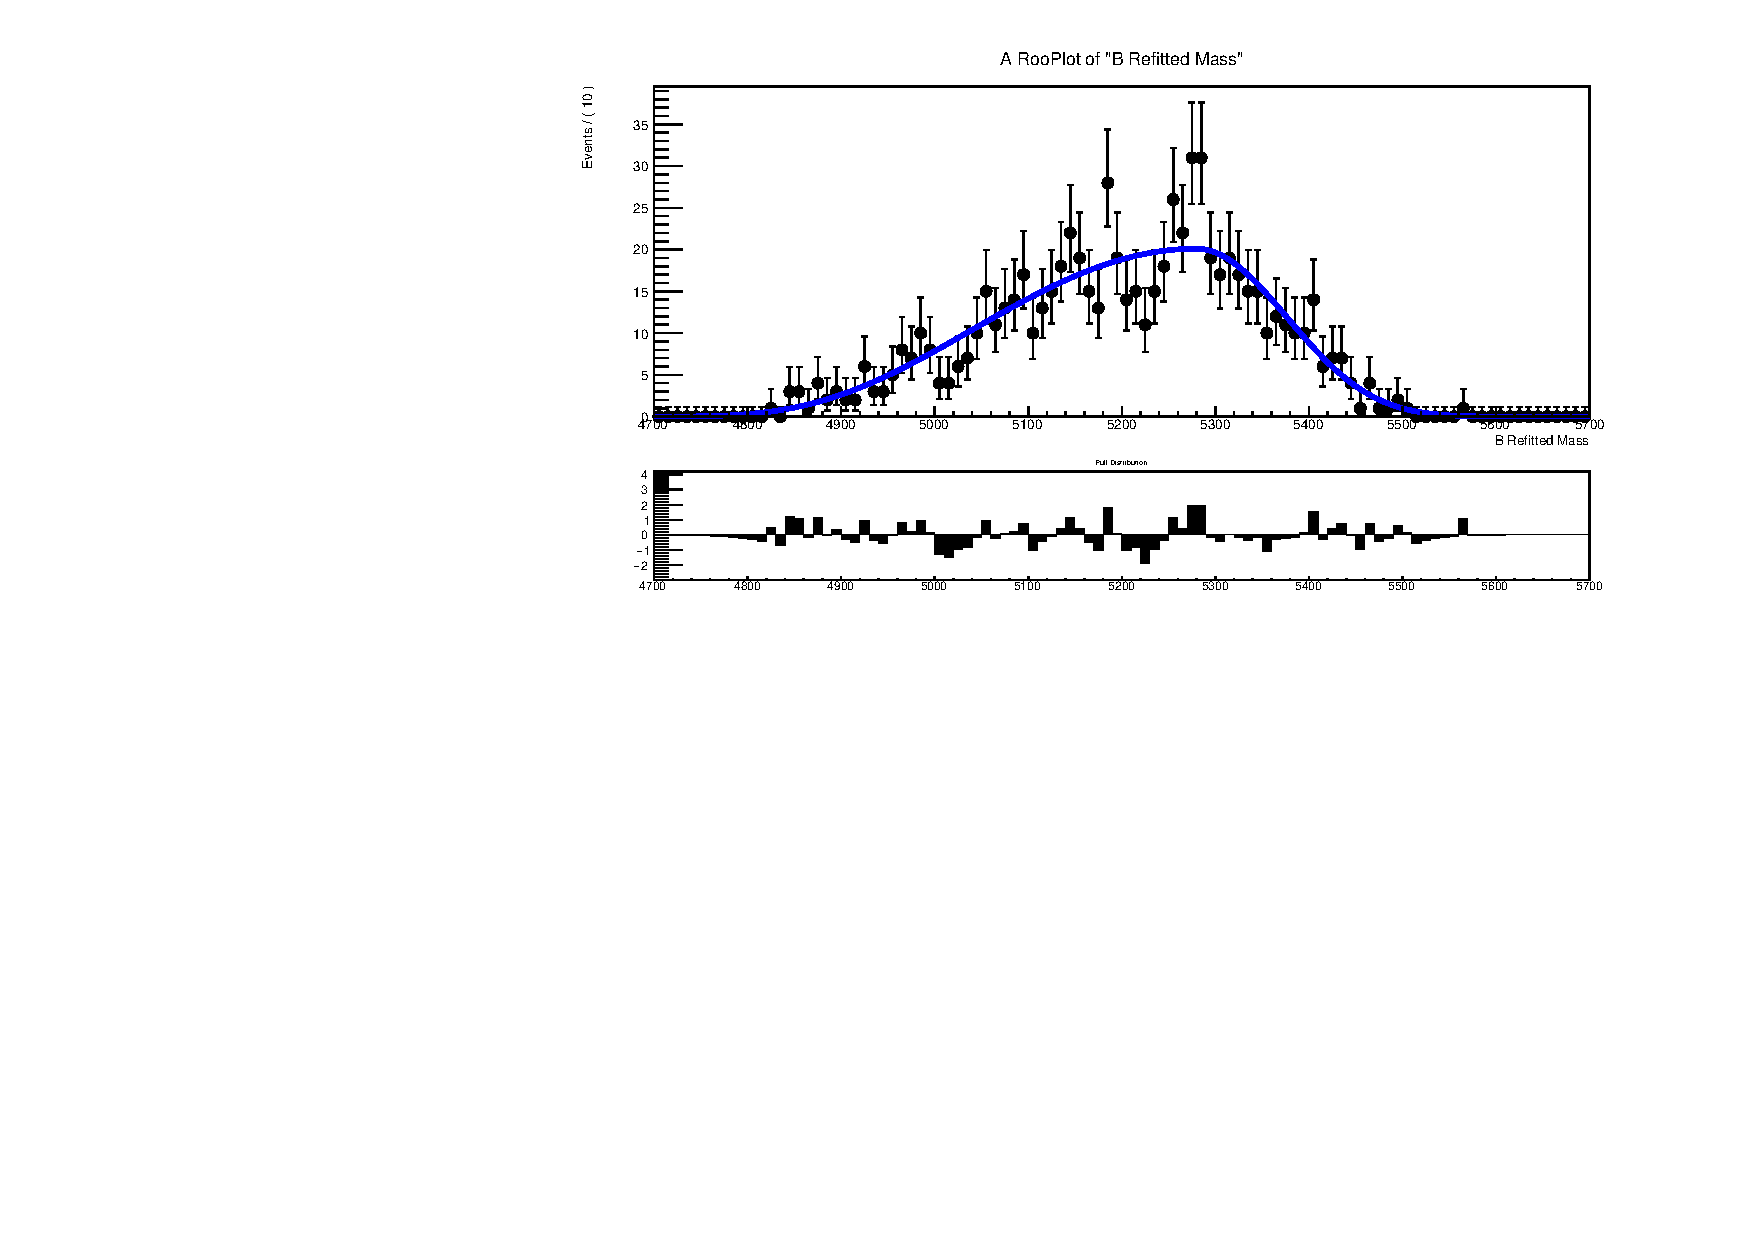
\includegraphics[width=0.7\linewidth]{figures/backgrounds/Lb2LcKst.pdf}
\caption{Fit to \decay{\Lb}{\Lc(pK\pi)\kaon} MC using a RooCruijff PDF, where the \pion is missed in reconstruction and the proton is misidentified as a kaon. This contributes as a source of background in the \decay{\Bm}{\D\Kstarm}, \decay{\D}{\Kp\Km} fit.}
\label{Lbfit}
\end{figure}

\begin{table}[h]
\centering
\begin{tabular}{cc}
\hline
Parameter & Value \\
\hline
$\mu$ & $5280 \pm 18$ \\
$\sigma_L$ & $221 \pm 26$ \\
$\sigma_R$ & $96 \pm 16$ \\
$\alpha_L$ & $-0.19 \pm 0.19$ \\
$\alpha_R$ & $-0.04 \pm 0.06$ \\
\hline
\end{tabular}
\caption{Shape parameters from a fit to \decay{\Lb}{\Lc\kaon} MC using a RooCruijff PDF. These shape parameters are fixed with an associated systematic uncertainty.}
\label{fitresultsLb}
\end{table}

The shape is assumed to be the same in each \decay{\D}{\Kp\Km} fit category. The \decay{\Lb}{\Lc\Kstar}, \decay{\Lc}{p\kaon\pi} yield compared to the signal yield in the favoured \decay{\Bm}{\D\Kstarm}, \decay{\D}{\Kp\Km} mode is allowed to vary in the fit. This fractional yield is the same for all fit categories. 

\subsubsection{Lambda contamination}
\label{sec:backgrounds:contamination}

The \decay{\KS}{\pip\pim} decay could have contamination coming from \decay{\Lz}{\proton\pim}, where the proton is reconstructed as a pion. It is not possible to determine possible \Lz contamination from the \KS invariant mass spectrum, where one of the \KS daughters is assigned the proton mass, because a peak at the \Lz mass cannot be distinguished from the variation near the low mass threshold. In order to distinguish between \KS decays and \Lz contamination the Armenteros-Podolanski (AP) plot is used~\cite{APplot}. The transverse momentum of the daughters with respect to the mother particle, $p_T$, is plotted against the longitudinal momentum asymmetry, which is defined as,

\begin{equation}
\frac{p_L^+ - p_L^-}{p_L^+ + p_L^-}
\end{equation}

where $p_L^{\pm}$ is the longitudinal momentum of the daughter particles with respect to the direction of the mother. The resulting AP plots for both data and MC are shown in Figure \ref{applots}. Both the data and MC samples have passed the full selection, except the MC sample does not have any PID applied. The decay products of the \decay{\KS}{\pip\pim} decay have the same mass and therefore on average their momenta is symmetrically distributed, resulting in the distribution observed in Figure \ref{applots}; these curves are the same shape as the expected distribution for a sample of pure \KS mesons. The distribution of the events in the data sample can be seen more clearly in Figure \ref{applotsdata}. Whereas for the \decay{\Lz}{\proton\pim}, the proton would, on average, take a larger proportion of the momentum resulting in an asymmteric distribution. Contamination from \Lz baryons would be clearly seen as a distinct structure on the AP plot, as illustrated in Figure \ref{apexample}. Therefore, Figure \ref{applots} shows that there is no contamination from \decay{\Lz}{\proton\pim} decays in this sample.

\begin{figure}[h]
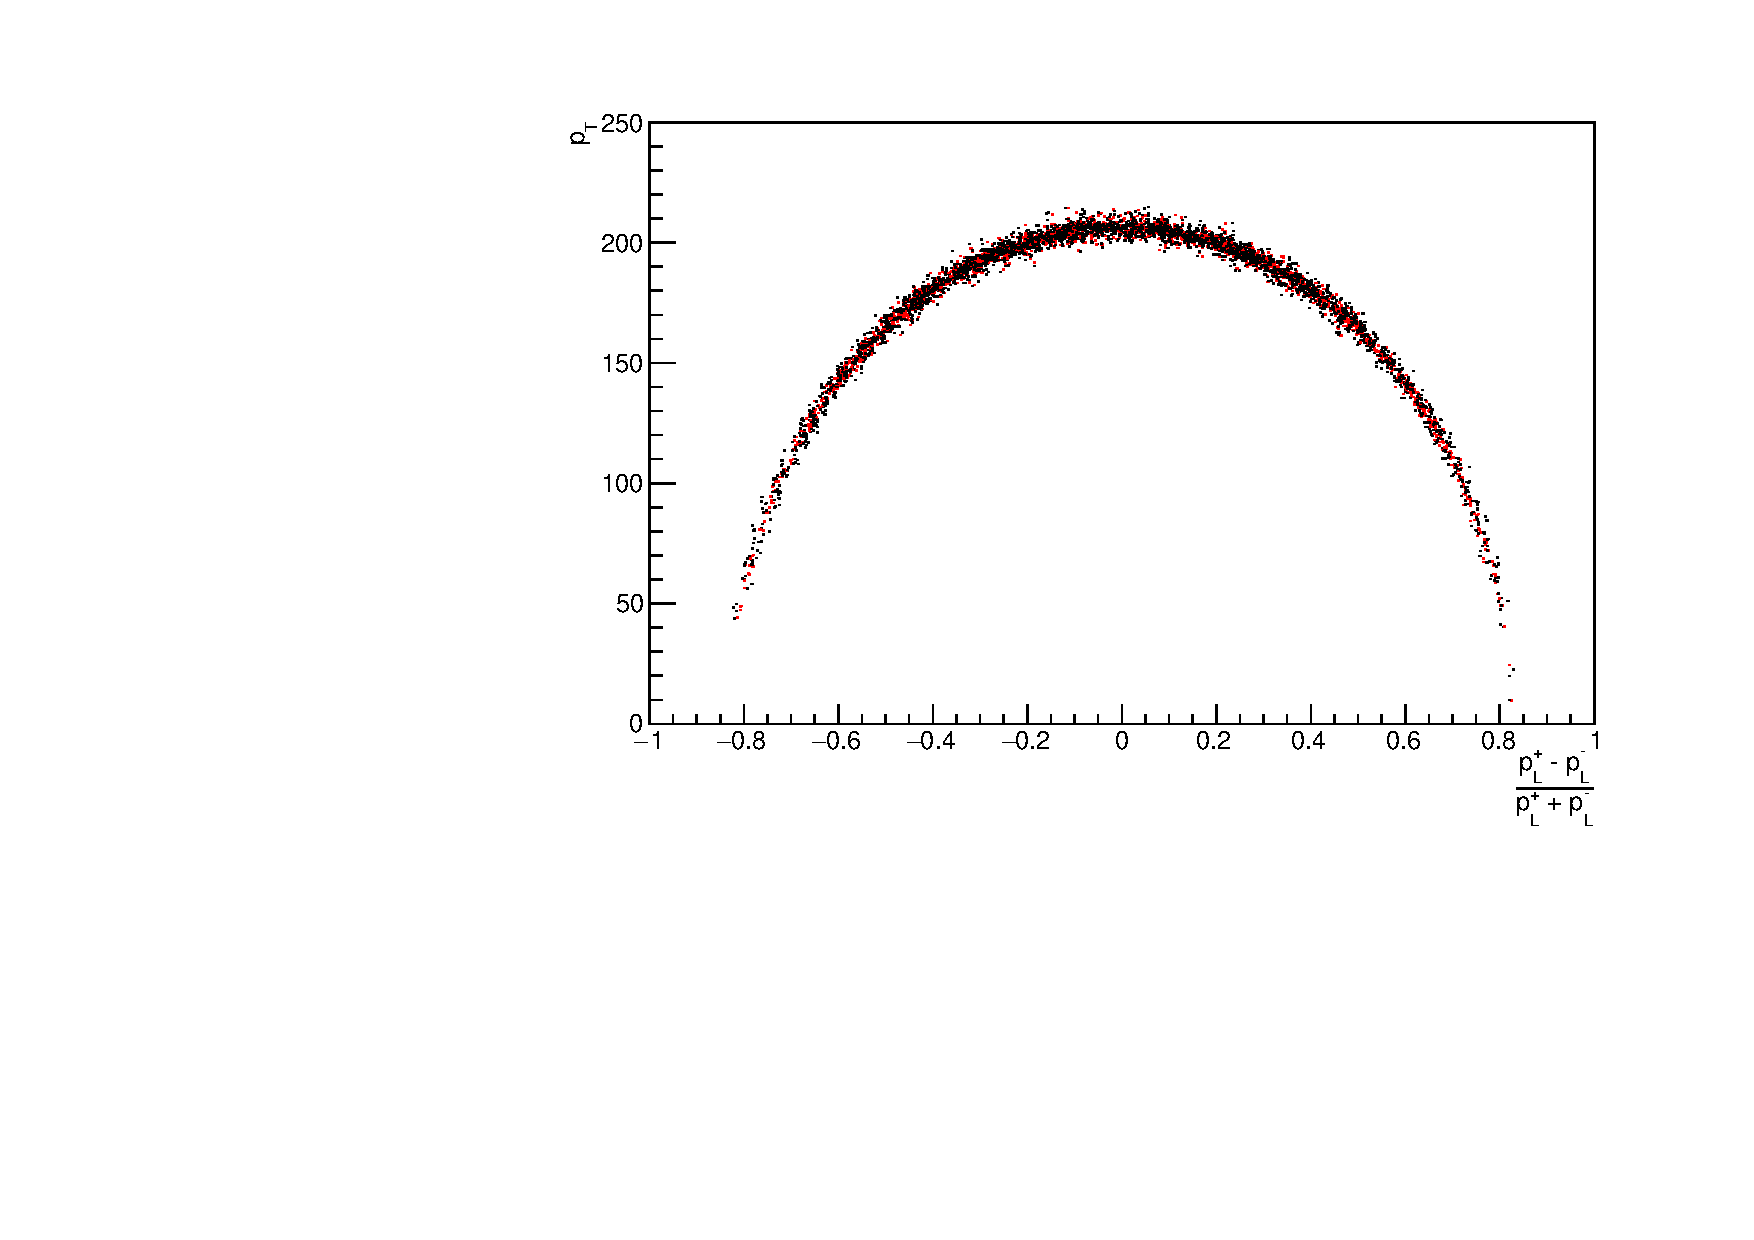
\includegraphics[width=0.5\linewidth]{figures/backgrounds/APplot_LL.pdf}
\put(-190,120) {(a)}
\hfill
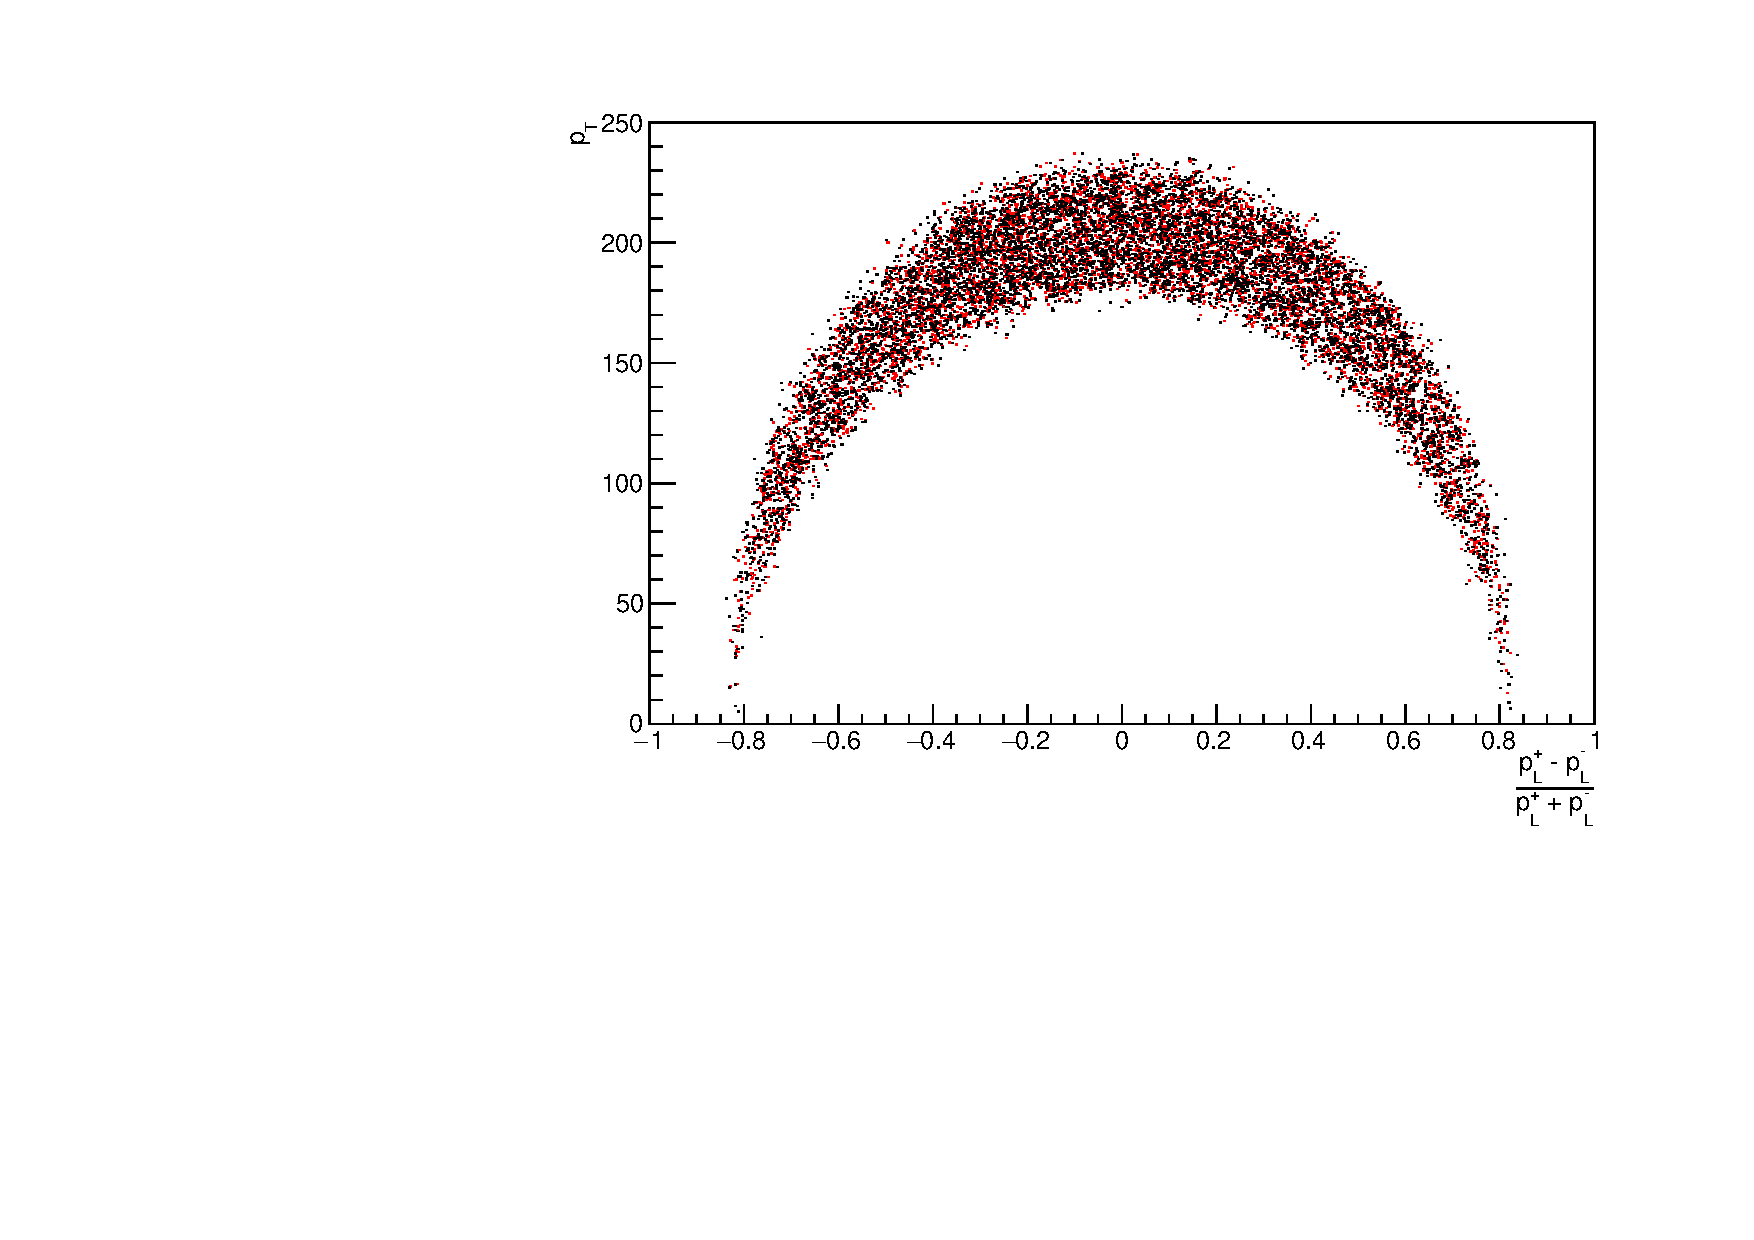
\includegraphics[width=0.5\linewidth]{figures/backgrounds/APplot_DD.pdf}
\put(-190,120) {(b)}
\caption{Armenteros-Podolanski plots for (a) LL, and (b) DD canididates. The $p_T$ values on the y axis are the transverse momentum of the daughters with respect to the mother particle and the x axis contains the longitudinal momentum asymmetry. The black points represent data and the red points represent MC.}
\label{applotsdata}
\end{figure}

\begin{figure}
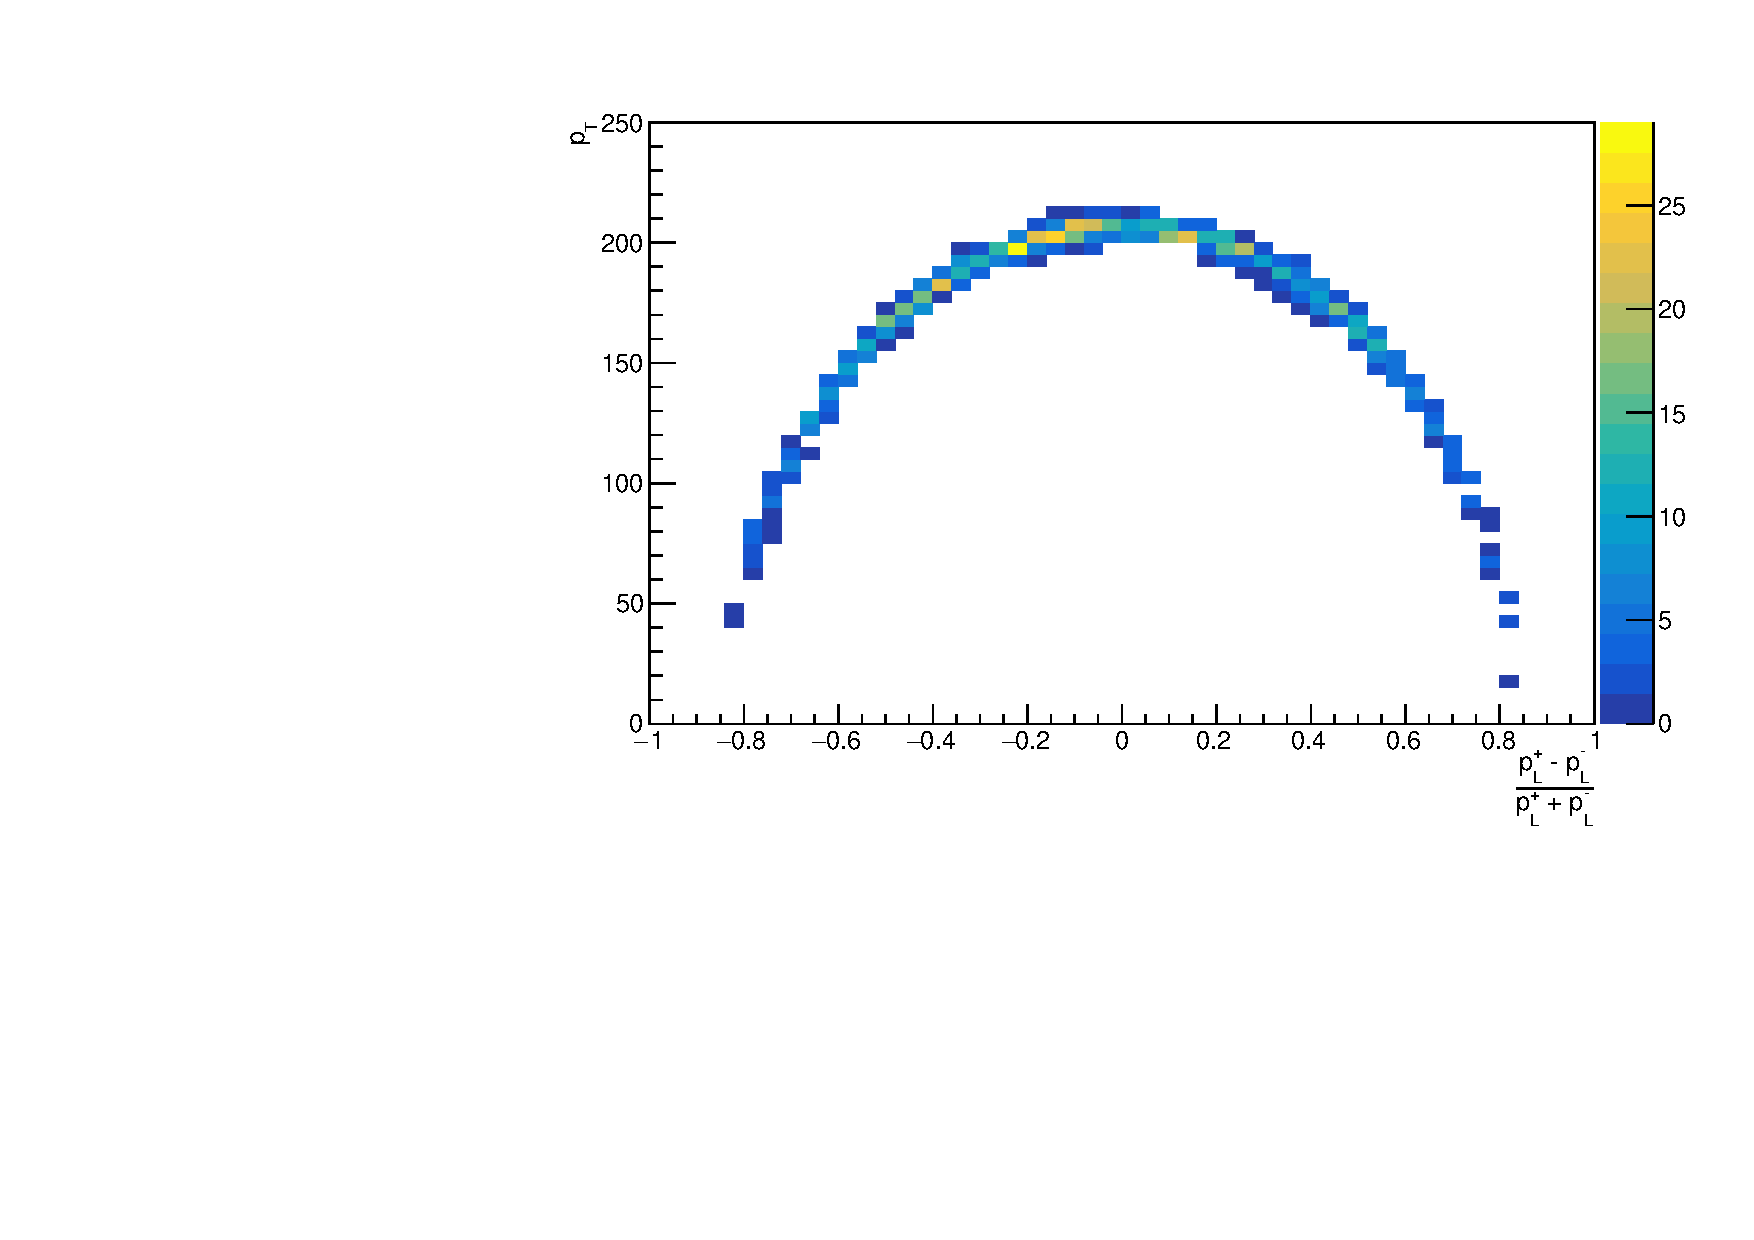
\includegraphics[width=0.5\linewidth]{figures/backgrounds/APplot_dataLL.pdf}
\put(-190,120) {(a)}
\hfill
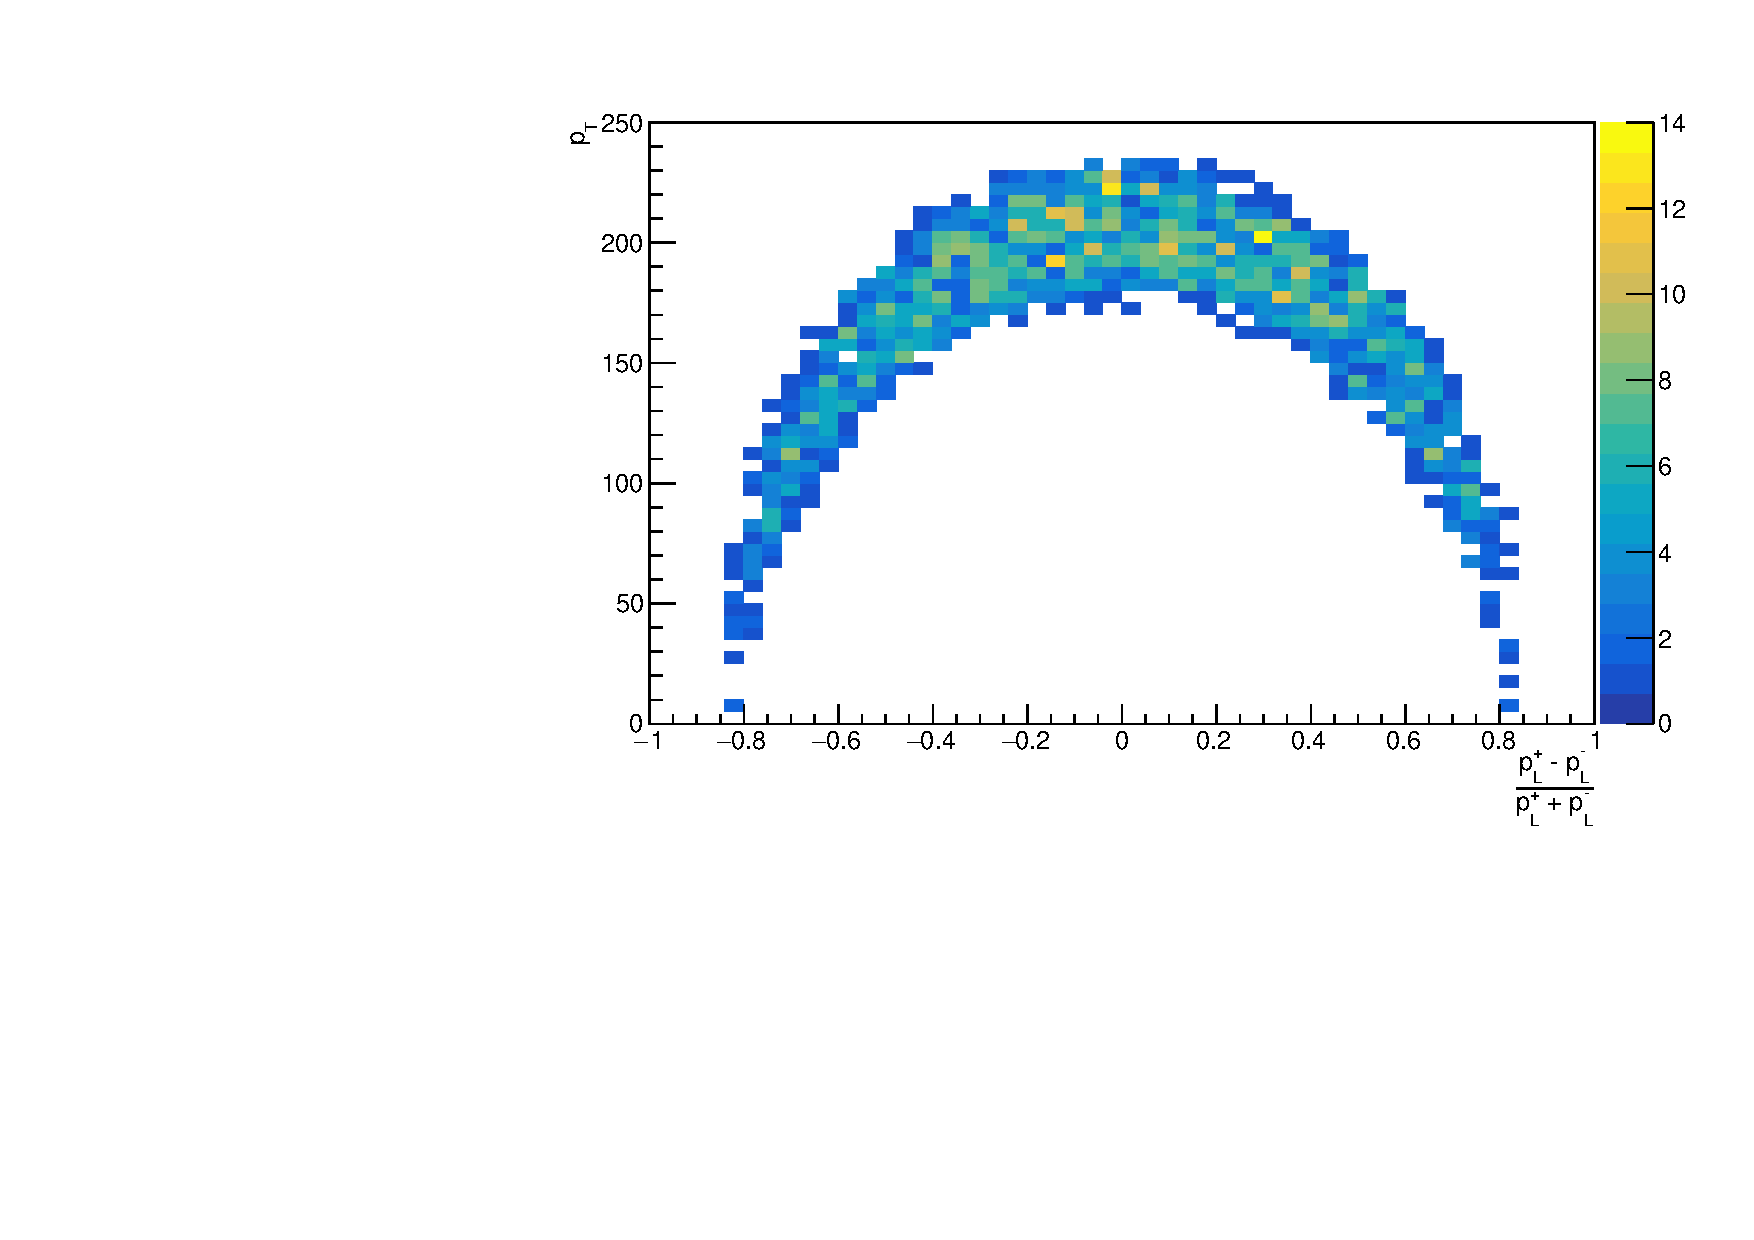
\includegraphics[width=0.5\linewidth]{figures/backgrounds/APplot_dataDD.pdf}
\put(-190,120) {(b)}
\caption{Armenteros-Podolanski plots for (a) LL, and (b) DD canididates in data. The $p_T$ values on the y axis are the transverse momentum of the daughters with respect to the mother particle and the x axis contains the longitudinal momentum asymmetry. The black points represent data and the red points represent MC.}
\label{applots}
\end{figure}

\begin{figure}
\centering
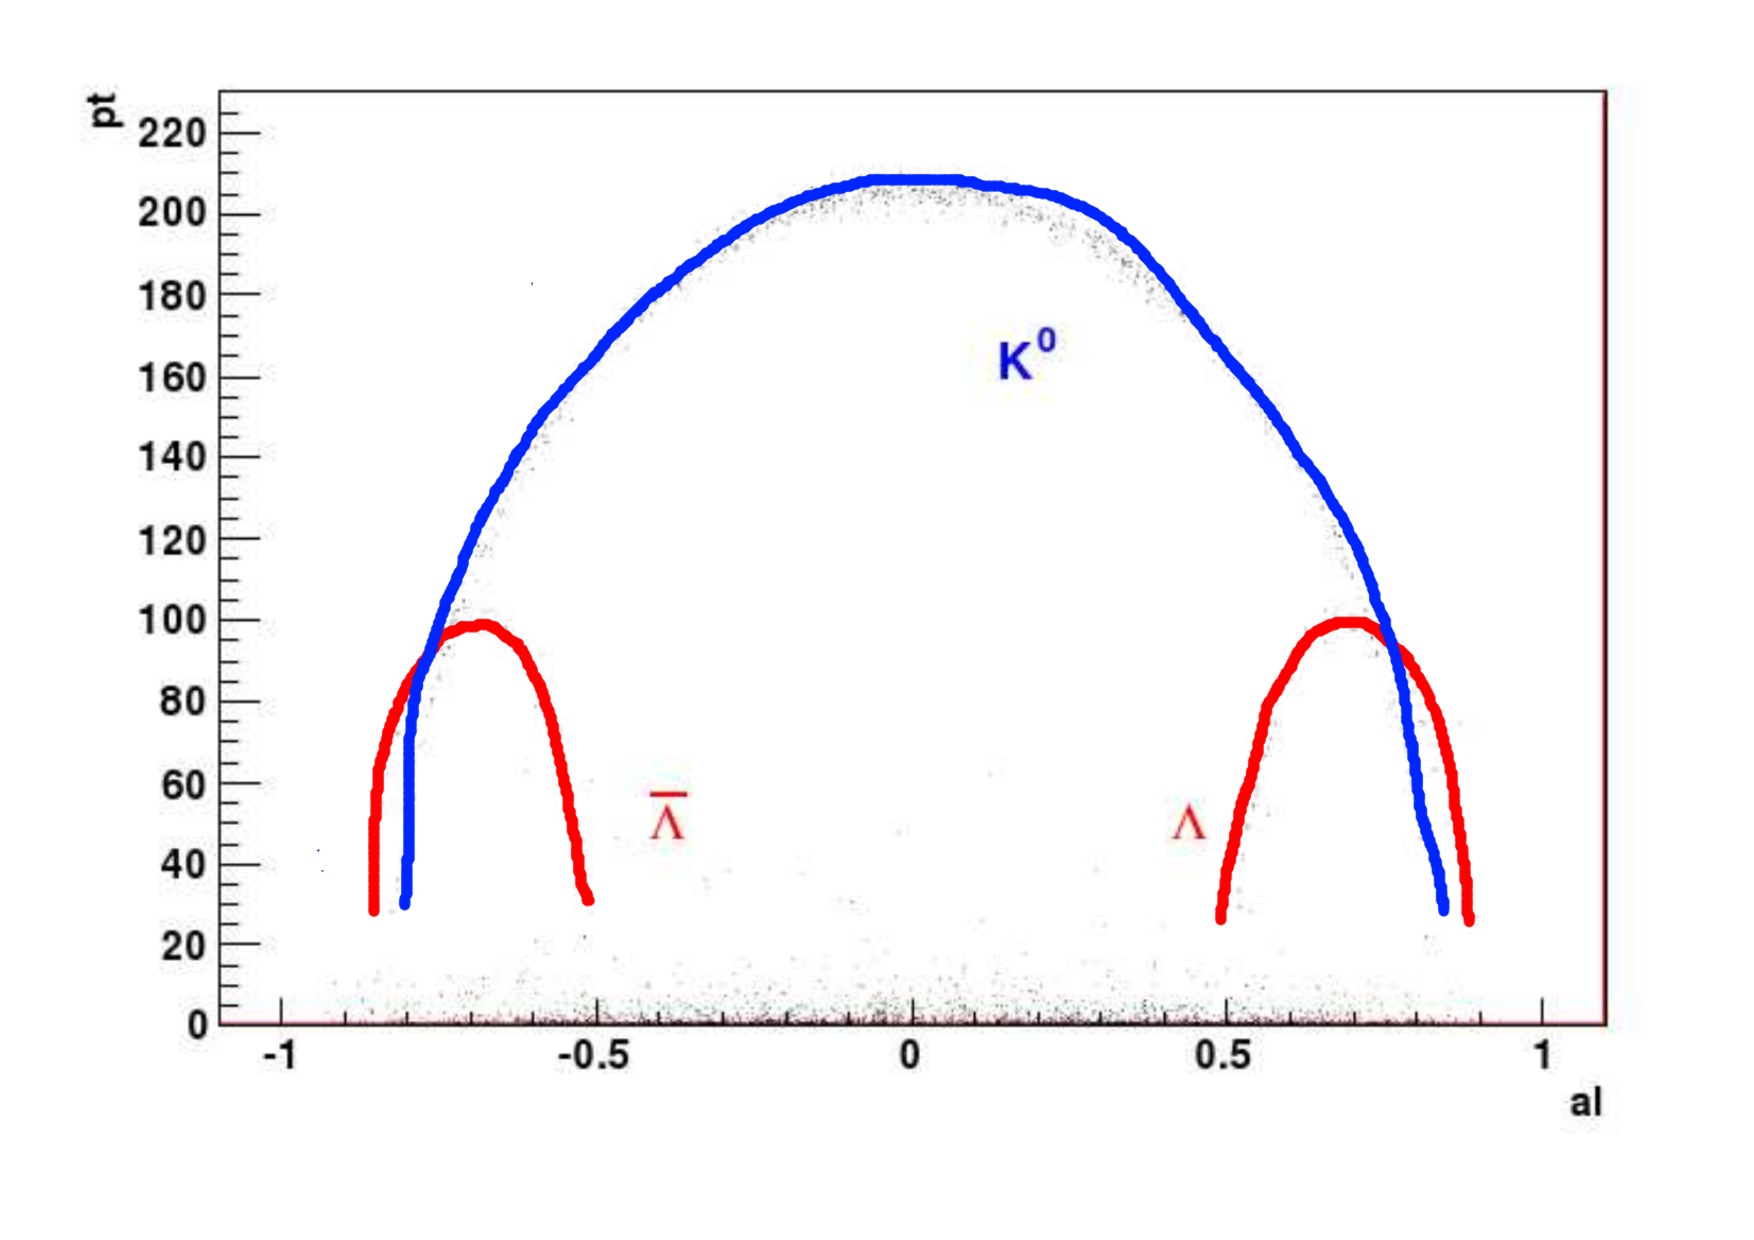
\includegraphics[width=0.5\linewidth]{figures/backgrounds/APfromPaper2.pdf}
\caption{An example Armenteros-Podolanski plot showing where the signal regions for \KS, \Lz and \Lbar are located in the AP plane~\cite{APplot}}
\label{apexample}
\end{figure}

\subsubsection{\decay{\B}{\D\KS\kaon}}
\label{sec:backgrounds:b2dkks}

The decay \decay{\B}{\D\KS\kaon} has a branching fraction of $5.5 \times 10^{-4}$~\cite{PDG2014}, which is similar to the signal branching fraction. However, nearly all of this background is removed by the 75 MeV \Kstarpm mass window and the DLLK $<$ 4 requirement on the bachelor pion. Table \ref{b2dkkspid} shows the rate of misidentification of the bachelor pion for \decay{\B}{\D\KS\kaon} MC.

\begin{table}[h]
\centering
\begin{tabular}{c|cc|cc}
\hline
& \multicolumn{2}{c}{LL} & \multicolumn{2}{c}{DD} \\
& MagUp & MagDown & MagUp & MagDown \\
\hline
2012 & $8.9 \pm 0.2$ & $8.1 \pm 0.2$ & $8.3 \pm 0.2$ & $8.0 \pm 0.2$ \\
2015 & $8.5 \pm 0.2$ & $9.7 \pm 0.2$ & $7.8 \pm 0.2$ & $7.4 \pm 0.2$ \\
\hline
Average Run 1 & \multicolumn{2}{c}{$8.5 \pm 0.3$} & \multicolumn{2}{c}{$8.2 \pm 0.3$} \\
Average Run 2 & \multicolumn{2}{c}{$9.1 \pm 0.2$} & \multicolumn{2}{c}{$7.6 \pm 0.3$} \\
\hline
\end{tabular}
\caption{MisID efficiencies for $B \to DK_sK$. The values in the table are given as percentages.}
\label{b2dkkspid}
\end{table}

Table \ref{b2dkkspid} shows that by requiring DLLK $<$ 4 on the bachelor pion the background is supressed to about 8\%. The efficiency of the 75 MeV \Kstarpm mass window when applied to \decay{\B}{\D\KS\kaon} MC is 3\% for both LL and DD. Combined misID rate and selection efficiencies means the decay is negligible even if the PID performance in Run 2 is not identical. Any residual amount is investigated alongside the systematics for the residual low mass background in this region.


\subsubsection{Other backgrounds}

Other backgrounds have been looked into and shown to have negligible contribution; a summary of these is given in Table \ref{ignoredbackgrounds}. No branching ratio has been measured for \decay{\Bm}{\Dz\Kstarm\piz} and \decay{\Bs}{\Dz\KS\pi\pi}, upper limits are guestimated hence this gives further motivation for restricting the mass range to 5230 \mevcc. As these backgrounds are estimated to have a low contribution in an area outside the mass range chosen for the \CP fit, they are considered negligible.

\begin{table}[h]
\centering
\begin{tabular}{cccc}
\hline
Decay mode & BR & Events relative to signal yield & Mass range (MeV) \\
\hline
\decay{\Bm}{\Dz\Kstarm\piz} & $6 \times 10^{-4}$ & 0.037/0.049 & 4750-5150 \\
\decay{\Bs}{\Dz\KS\pi\pi} & $5 \times 10^{-4}$ & 0.004/0.003 & 4750-5120 \\
\hline
\end{tabular}
\caption{Summary of background that have been investigated and determined to be negligible. Relative number of events are given for LL and DD (LL/DD). Branching ratios are guestimated upper limits}
\label{ignoredbackgrounds}
\end{table}

%In the \decay{\B}{Dh} analysis~\cite{LHCb-PAPER-2016-003}, the background \decay{\Lb}{\Lcm(\proton\Kp[\pim])\Kp} enters into the \decay{\Dz}{\Kp\Km} mode. This is where the \pim is missed in the reconstruction and the \proton is misIDed as a \kaon, this results in the recontructed \B mass falling within the mass fit range. This was found to be negligible and not affect the 

Many other backgrounds have been looked into and have been found to be negligible:

\begin{itemize}
\item \decay{\Bs}{\Dzb\Kstarz(\Kstarp[\pim])}
\item \decay{\Bs}{\Dstarp\Kstarp}
\item \decay{\Bs}{\Dspm(\kaon\kaon\pi)\Kstarpm}
\item \decay{\Bu}{\D\pi} with a random \KS added
\item \decay{\Bd}{\D\KS} with a  random pion added
\item \decay{\Bs}{\D\KS} with a random pion added
\item \decay{\Bu}{\D(\KS\pi\pi)\Kp}
\item \decay{\Lb}{\Lambda_c^-(\proton\Kp[\pim])\Kstarp} with the \proton misIDed as a kaon
\end{itemize}


\subsection{PID selection}
\label{sec:selection:pid}

The selection requirements are identical for each of the different D modes, $K\pi$, $KK$, $\pi\pi$ and $\pi K$, with the exception of the double misID veto. Therefore, it is essential to apply PID selection that efficiently distinguishes between pions and kaons. The PID cuts on the daughters of the D meson are designed so that no \decay{\Dz}{hh} candidate can appear in more than one category with a change in mass hypothesis. A PID requirement must be made on the bachelor pion in order to remove the \decay{\B}{\D\KS\kaon} background; this is discussed in more detail in Section \ref{sec:backgrounds:b2dkks}. 

For the bachelor PID (pion coming from the \Kstarm) a requirement of PIDK $<$ 4 is applied. For the 2-body D modes the requirements on the D daughters are kaons must satisfy DLLK $>$ 2 and pions must satifsfy DLLK $<$ -2. For the \decay{\Dz}{K\pi\pi\pi} modes, e.g. \decay{\Dz}{\Km\pip\pim\pip}, the \Km must satisfy DLLK $>$ 2 and both \pip must satifsfy DLLK $<$ -2; no PID requirement is applied for the \pip. For the \decay{\Dz}{\pip\pim\pip\pim}, the two \pip mesons must satisfy DLLK $<$ -2 and no PID requirements is placed on the \pim mesons. The PID requirements are the same as those used in the \decay{\Bp}{\D\Kp} analysis~\cite{LHCb-PAPER-2016-003}. No PID requirements are made on the \KS daughters; the high purity of the \KS means that this is not necessary, this is justified in Section \ref{sec:backgrounds:contamination}. The efficiency of this PID selection for the $K\pi$ favoured mode in Run 1 is 74\% and the efficiency of $\pi K$ events in the favoured mode is 0.15\%. These efficiencies are discussed in more detail in Section \ref{sec:cpfit:efficiencies:pid}. 


A brief look at ProbNN variables was undertaken early on in the analysis but cuts were not found that improved on the DLL cuts. Figure \ref{pidoptimisation} shows the variation of PID efficiencies with different selections. These results are based on a preliminary version of the selection and so the DLLK efficiencies are not the same as those quoted in this analysis.  The same PID selection is applied to both Run 1 and Run 2 datasets. It was found that for the given PID selection both PID efficiency and misID efficiency were improved for Run 2 compared to Run 1. More detail is given in Section \ref{sec:cpfit:efficiencies:pid}.

\begin{figure}
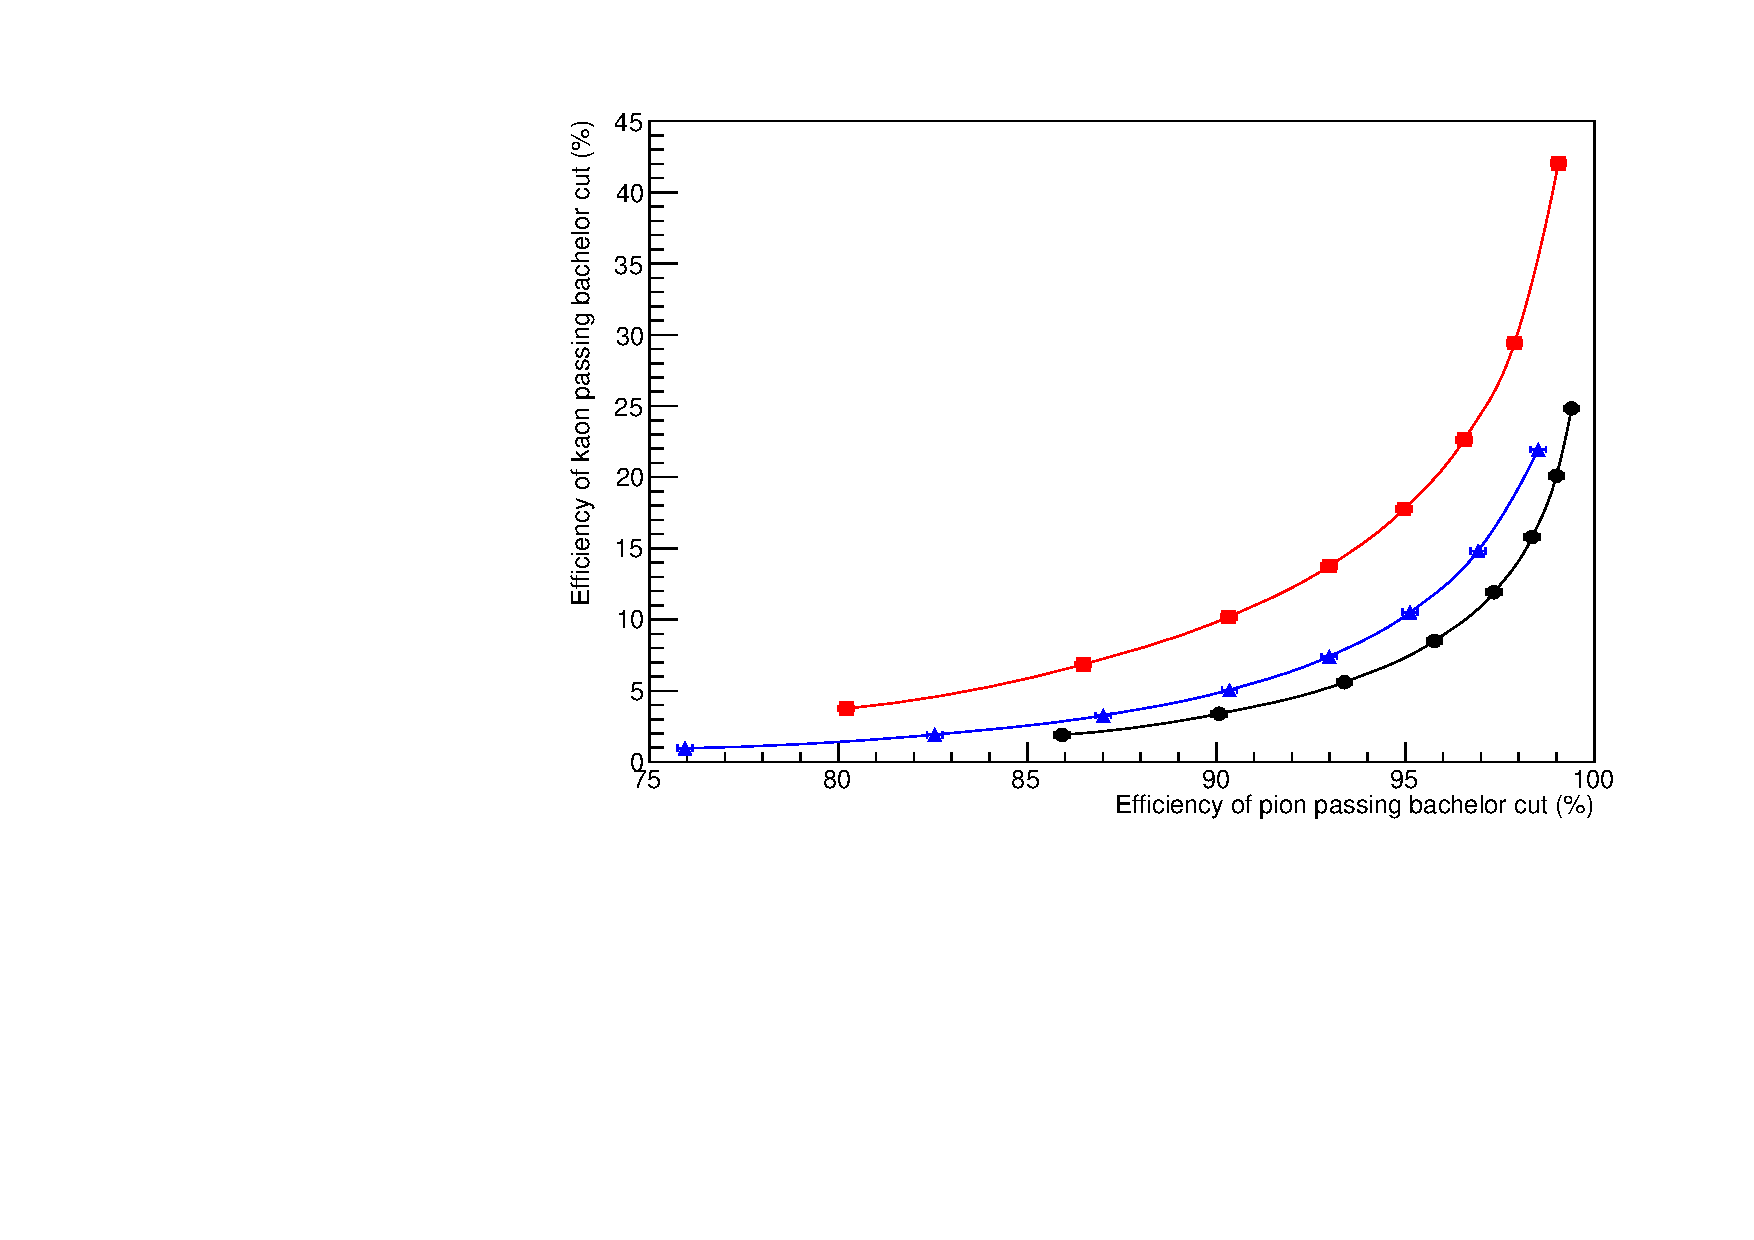
\includegraphics[width=0.5\linewidth]{figures/selection/pidOptimisation_bachelor.pdf}
\put(-150,100) {(a)}
\hfill
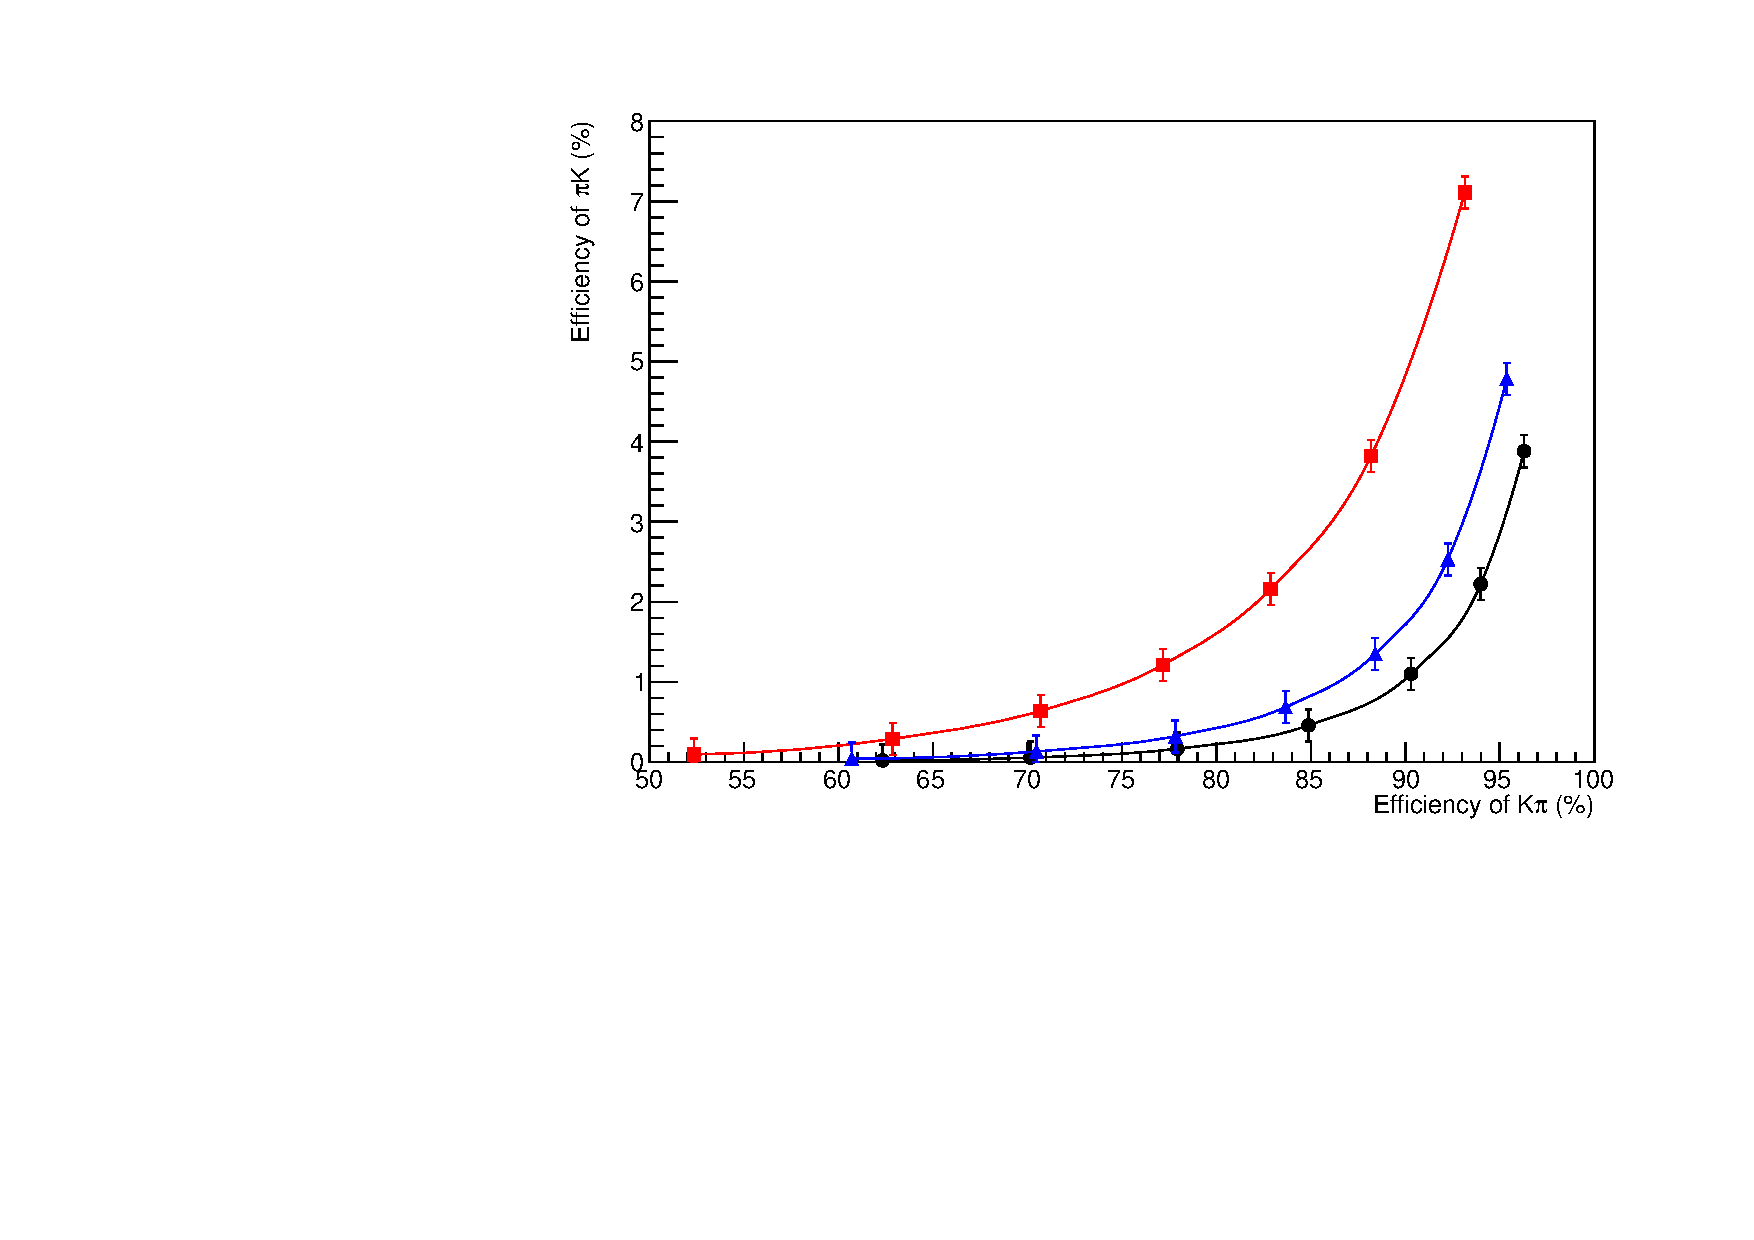
\includegraphics[width=0.5\linewidth]{figures/selection/pidOptimisation_Ddaughters.pdf}
\put(-150,100) {(b)}
\caption{PID efficiencies and misID efficiencies for various PID selections applied to (a) the bachelor pion, and (b) the D daughters. The black curve is for selections using $DLLK$, the red curve is for selections using $ProbNNpi$ and the blue curve is for selections using $ProbNNpi \times (1-ProbNNk)$}
\label{pidoptimisation}
\end{figure}

\subsection{Multiple candidates}
\label{sec:selection:multiplecandidates}

The selection may produce more than one signal event from the same B candidate. The rate of these multiple candidates was calculated after the final selection and only considering candidates in the range of the \CP fit (refitted \B mass $>$ 5230 \mev), see Section \ref{sec:massfit:range} for details on the fit range. The results are shown in Tables \ref{multiplecandidatesRun1} and \ref{multiplecandidatesRun2}. The rate is so low that no action is taken to remove the multiple candidates. In the ADS mode where it would have a significant effect, there are no multiple candidates.

\begin{table}[h]
\centering
\begin{tabular}{ccc}
\hline
& LL & DD \\
\hline
$K\pi$ & 0.005 (4) & 0.004 (9) \\
$K\pi$ & 0.008 (2) & 0.005 (3) \\
$KK$ & 0 (0) & 0 (0) \\
$\pi\pi$ & 0 (0) & 0 (0) \\
$\pi K$ & 0 (0) & 0 (0) \\
$K\pi\pi\pi$ & 0 (0) & 0.026 (7) \\
$\pi K\pi\pi$ & 0 (0) & 0.05 (1) \\
\hline
\end{tabular}
\caption{Multiple candidate rate for Run1. The number in brackets is the actual number of multiple candidates}
\label{multiplecandidatesRun1}
\end{table}

\begin{table}[h]
\centering
\begin{tabular}{ccc}
\hline
& LL & DD \\
\hline
$K\pi$ & 0.005 (7) & 0.005 (19) \\
$K\pi$ & 0.005 (2) & 0.004 (5) \\
$KK$ & 0 (0) & 0.006 (1) \\
$\pi\pi$ & 0 (0) & 0.011 (1) \\
$\pi K$ & 0 (0) & 0 (0) \\
$K\pi\pi\pi$ & 0 (0) & 0.012 (9) \\
$\pi K\pi\pi$ & 0 (0) & 0 (0) \\
\hline
\end{tabular}
\caption{Multiple candidate rate for Run 2. The number in brackets is the actual number of multiple candidates}
\label{multiplecandidatesRun2}
\end{table}

\clearpage

\section{Mass parameterisation of the favoured mode}
\label{sec:massfit}

This section describes the mass parameterisation that is developed for the two and four-body favoured \D modes, namely \decay{\Bm}{\D(\Km\pip)\Kstarm} and \decay{\Bm}{\D(\Km\pip\pim\pip)\Kstarm}. The fit to data is performed on the refitted invariant mass of \B candidates. The aim is to parameterise the invariant \B mass to be used in the simultaneous fit described in Section \ref{ch:5-cpfit} to extract the \CP observables. There are three components considered in the parameterisation of the mass shape:
\begin{enumerate}
\item Signal, \decay{\Bm}{\D\Kstarm} decays.
\item Combinatoric background, where random tracks are combined in the reconstruction 
\item Partially reconstructed background, where one particle has been missed in the reconstruction, for example \decay{\Bm}{(\decay{\Dstarz}{\Dz[\piz]})\Kstarm}, where the \piz is not reconstructed.
\end{enumerate}

The shape of each fit component, and any constraints in background yields imposed, is discussed in the following sections. The shapes for the LL and DD \KS categories are considered separately because of their different reconstructed \B mass resolutions.

\subsection{Signal shape}
\label{sec:massfit:signal}

The signal can be described as the sum of two Gaussians with low mass tails to account for radiative effects. These modified Gaussians are known as Crystal Ball (CB) functions~\cite{Skwarnicki:1986xj}. This Double Crystal Ball shape is defined in Equation \ref{DCBshape}. 
\begin{equation}
\mathrm{DCB}(m| \mu,\sigma,\alpha,n,f_{cb}) = f_{cb} \cdot \mathrm{CB}(m| \mu,\sigma,\alpha,n) + (1-f_{cb}) \cdot \mathrm{CB}(m|\mu,f_{\sigma}\sigma,\alpha,n),
\label{DCBshape}
\end{equation}
where
\begin{equation*}
  \mathrm{CB}(m| \mu,\sigma,\alpha,n)=
\begin{cases}
    e^{-((m-\mu)/ \sigma)^2/2},                                   & \text{if } \frac{m-\mu}{\sigma} \geq - \alpha, \\
   \left ( \frac{n}{|\alpha|} \right ) ^n e^{-|\alpha|^2/2} \left ( \frac{n}{|\alpha|} - |\alpha| - \left ( \frac{m-\mu}{\sigma} \right ) \right ) ^{-n} ,    & \text{otherwise.}
\end{cases}
\end{equation*}

Fits to the refitted \B mass distributions have been compared between \runone and \runtwo simulated signal samples, the signal PDFs are shown in Figures \ref{signalfitcomparison2body}. These shapes are consistent between \runone and \runtwo, therefore signal shapes are shared in the simultaneous fit. Further comparisons are made between two- and four-body modes. Figure \ref{signalfitcomparisonRun1} compare the signal PDFs obtained from simulated samples between $K\pi$ and $K\pi\pi\pi$ for \runone samples. These are noticablely different and so $K\pi$ and $K\pi\pi\pi$ are associated with different signal shapes in the mass fit.

\begin{figure}[h]
\centering
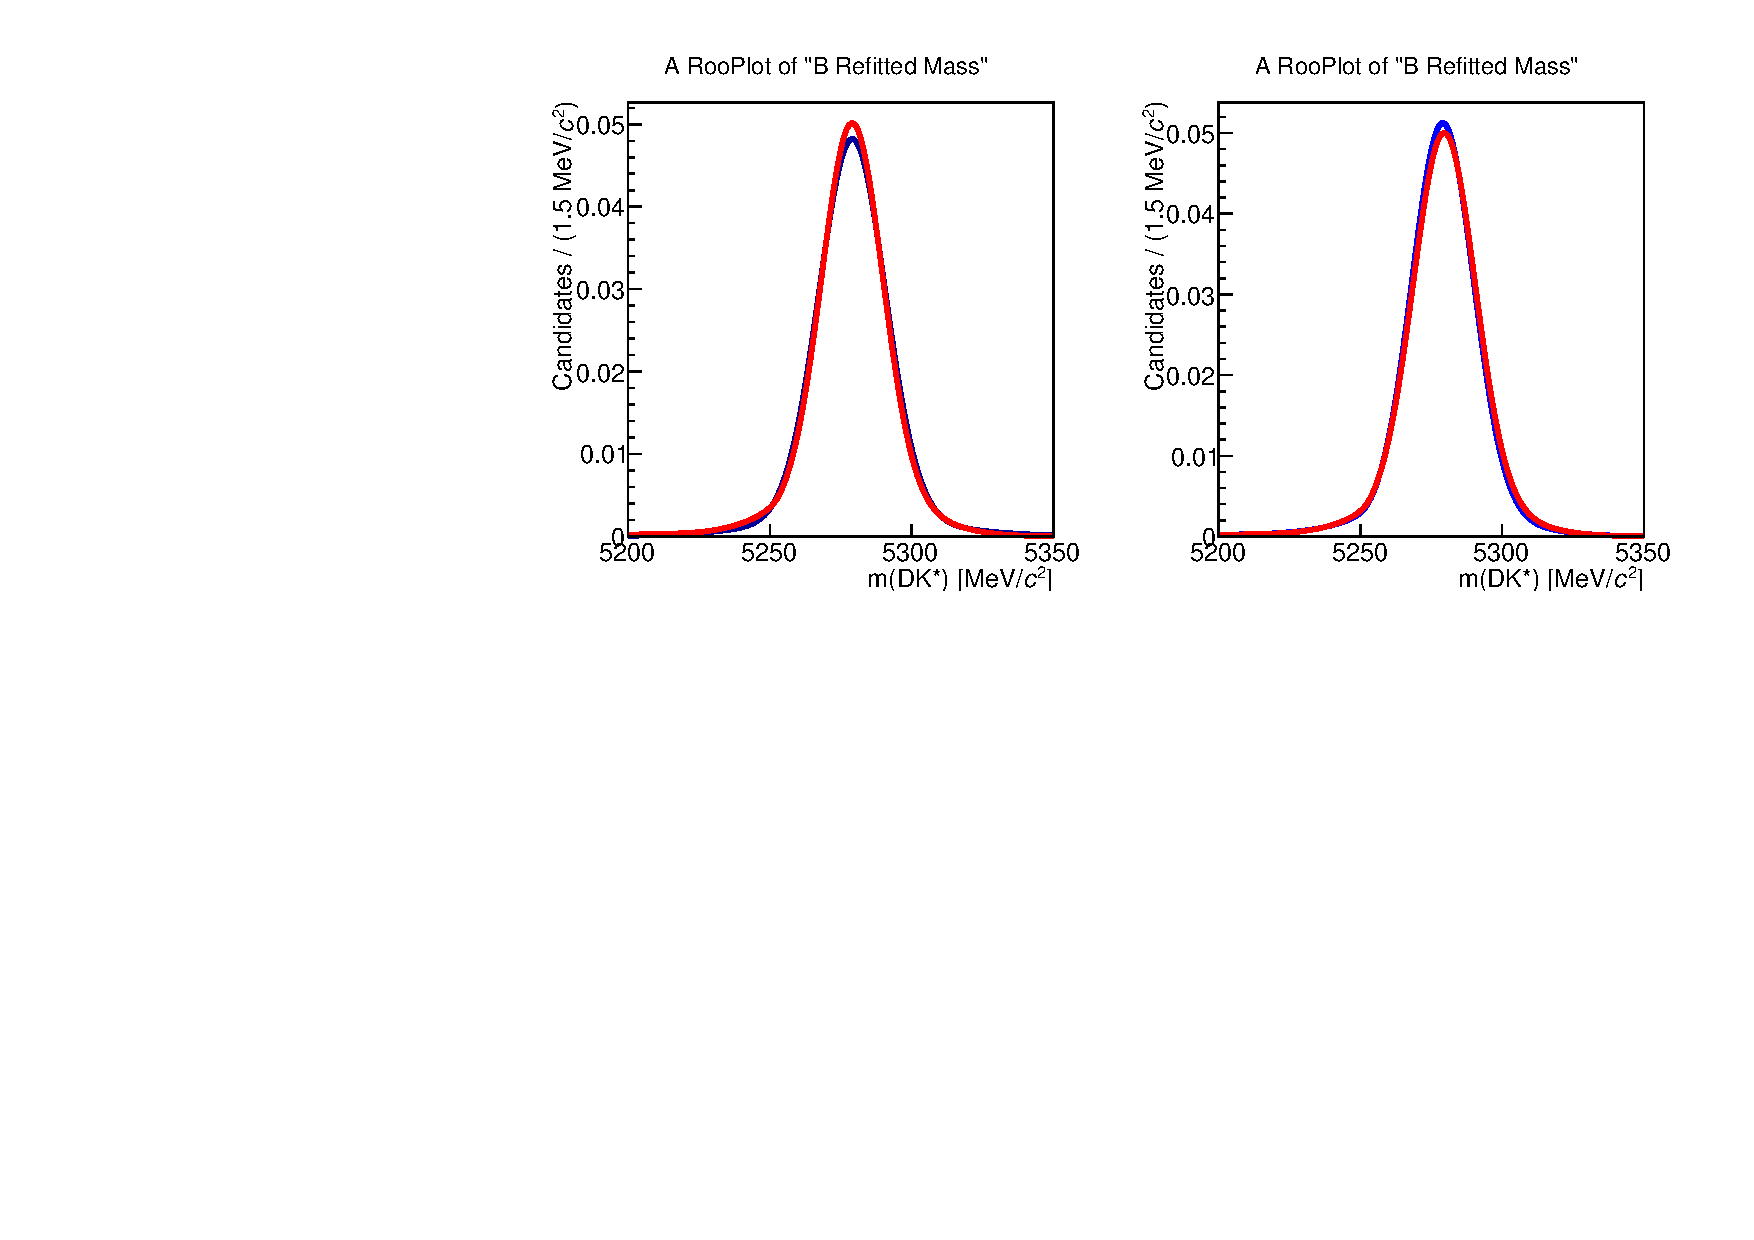
\includegraphics[width=0.7\linewidth]{figures/fitComponents/signalMC_KPi_run1vsrun2.pdf}
\put(-260,100) {(a)}
\put(-110,100) {(b)}
\caption{Comparison of $K\pi$ signal fit functions for \runone (blue) and \runtwo MC (red) for (a) LL candidates and (b) DD candidates}
\label{signalfitcomparison2body}
\end{figure}

\begin{figure}[h]
\centering
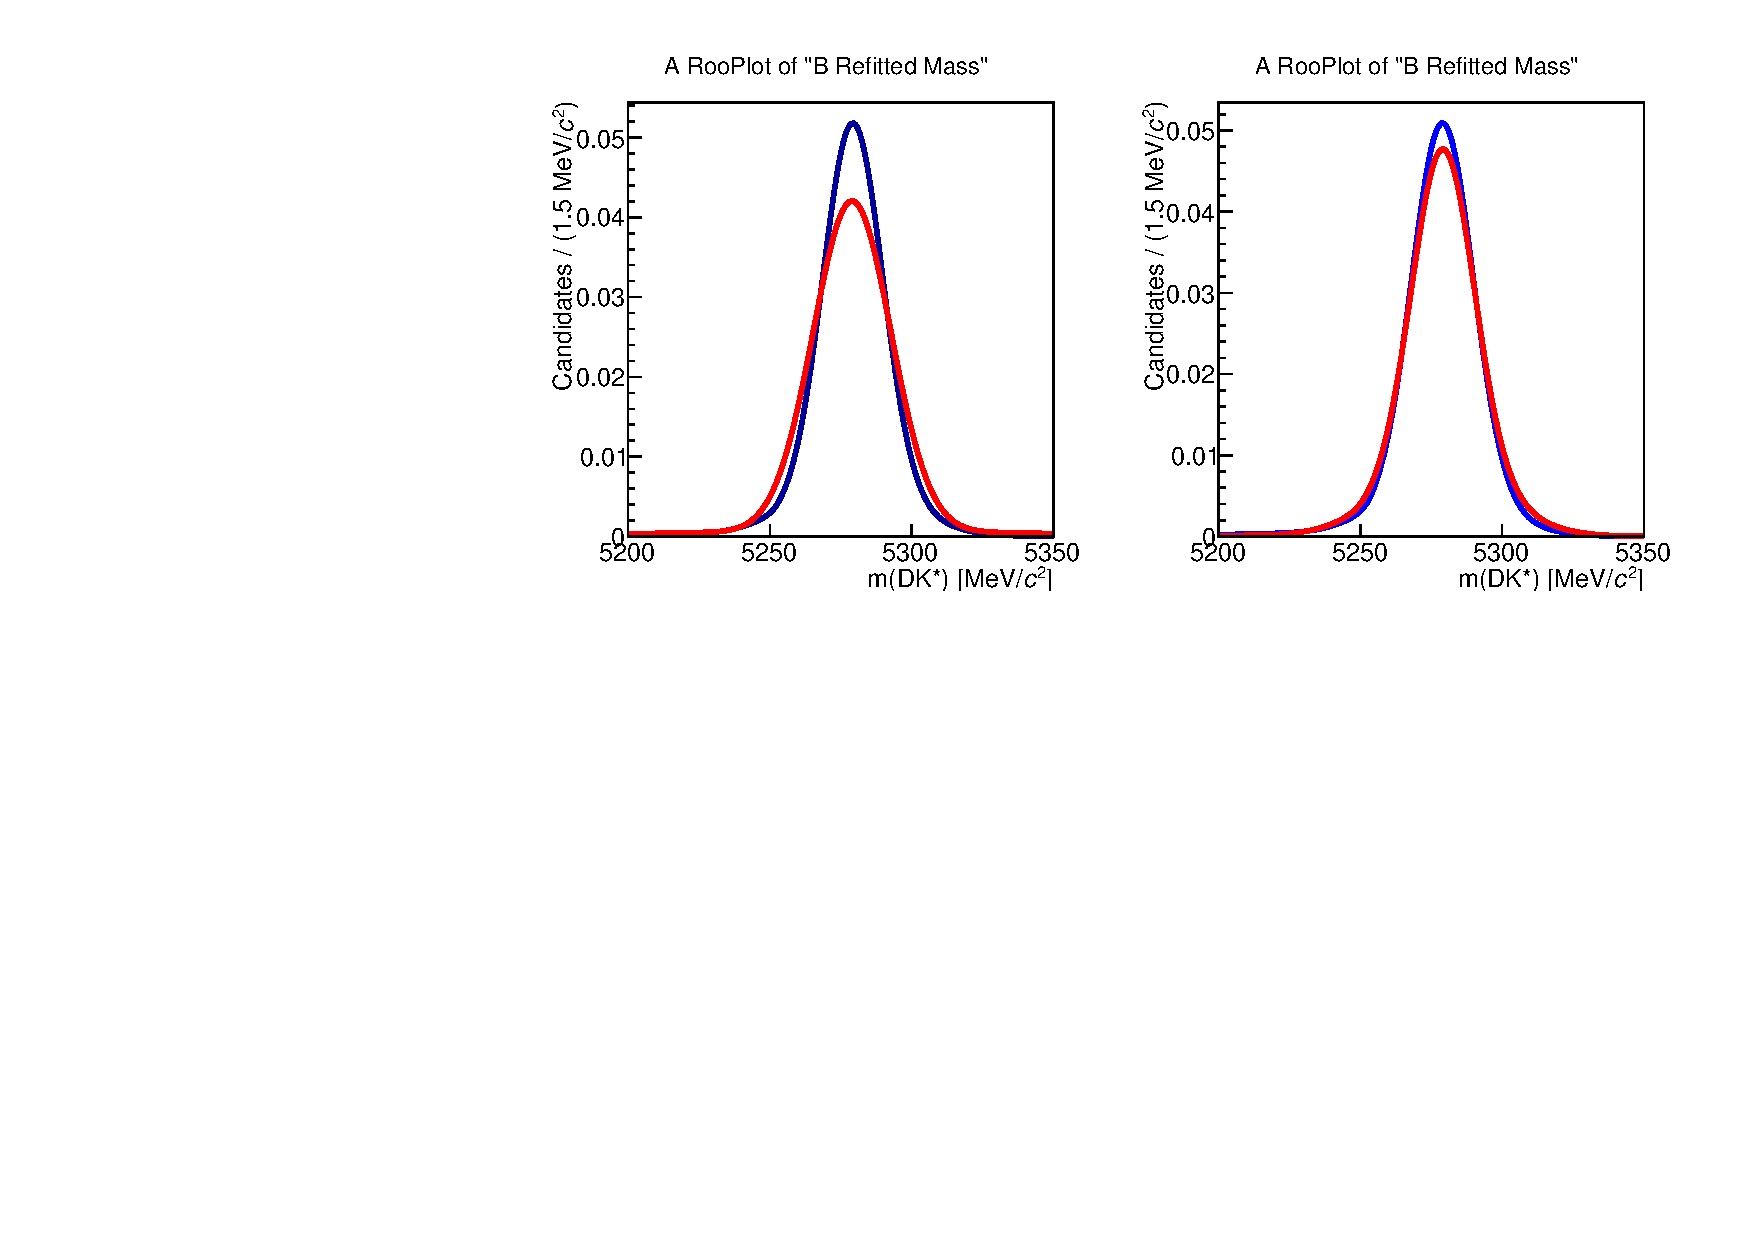
\includegraphics[width=0.7\linewidth]{figures/fitComponents/signalMC_run1_KPivsKPiPiPi.pdf}
\put(-260,100) {(a)}
\put(-110,100) {(b)}
\caption{Comparison of \runone signal fit functions for $K\pi$ (blue) and $K\pi\pi\pi$ (red) for (a) LL candidates and (b) DD candidates}
\label{signalfitcomparisonRun1}
\end{figure}

For the signal shape in the mass fit, the tail parameters, $\alpha$ and $n$, are fixed from simulation and both CBs share the same mean and tail parameters.  The width fraction between the CBs, $f_{\sigma}$, is fixed from simulation, but the mean and width, $\mu$ and $\sigma$, are left floating. The fits to simulated signal samples are shown in Figure \ref{signalfits} and the shape parameters obtained from these fits are detailed in Table \ref{signalparameters}. 

\begin{figure}[h]
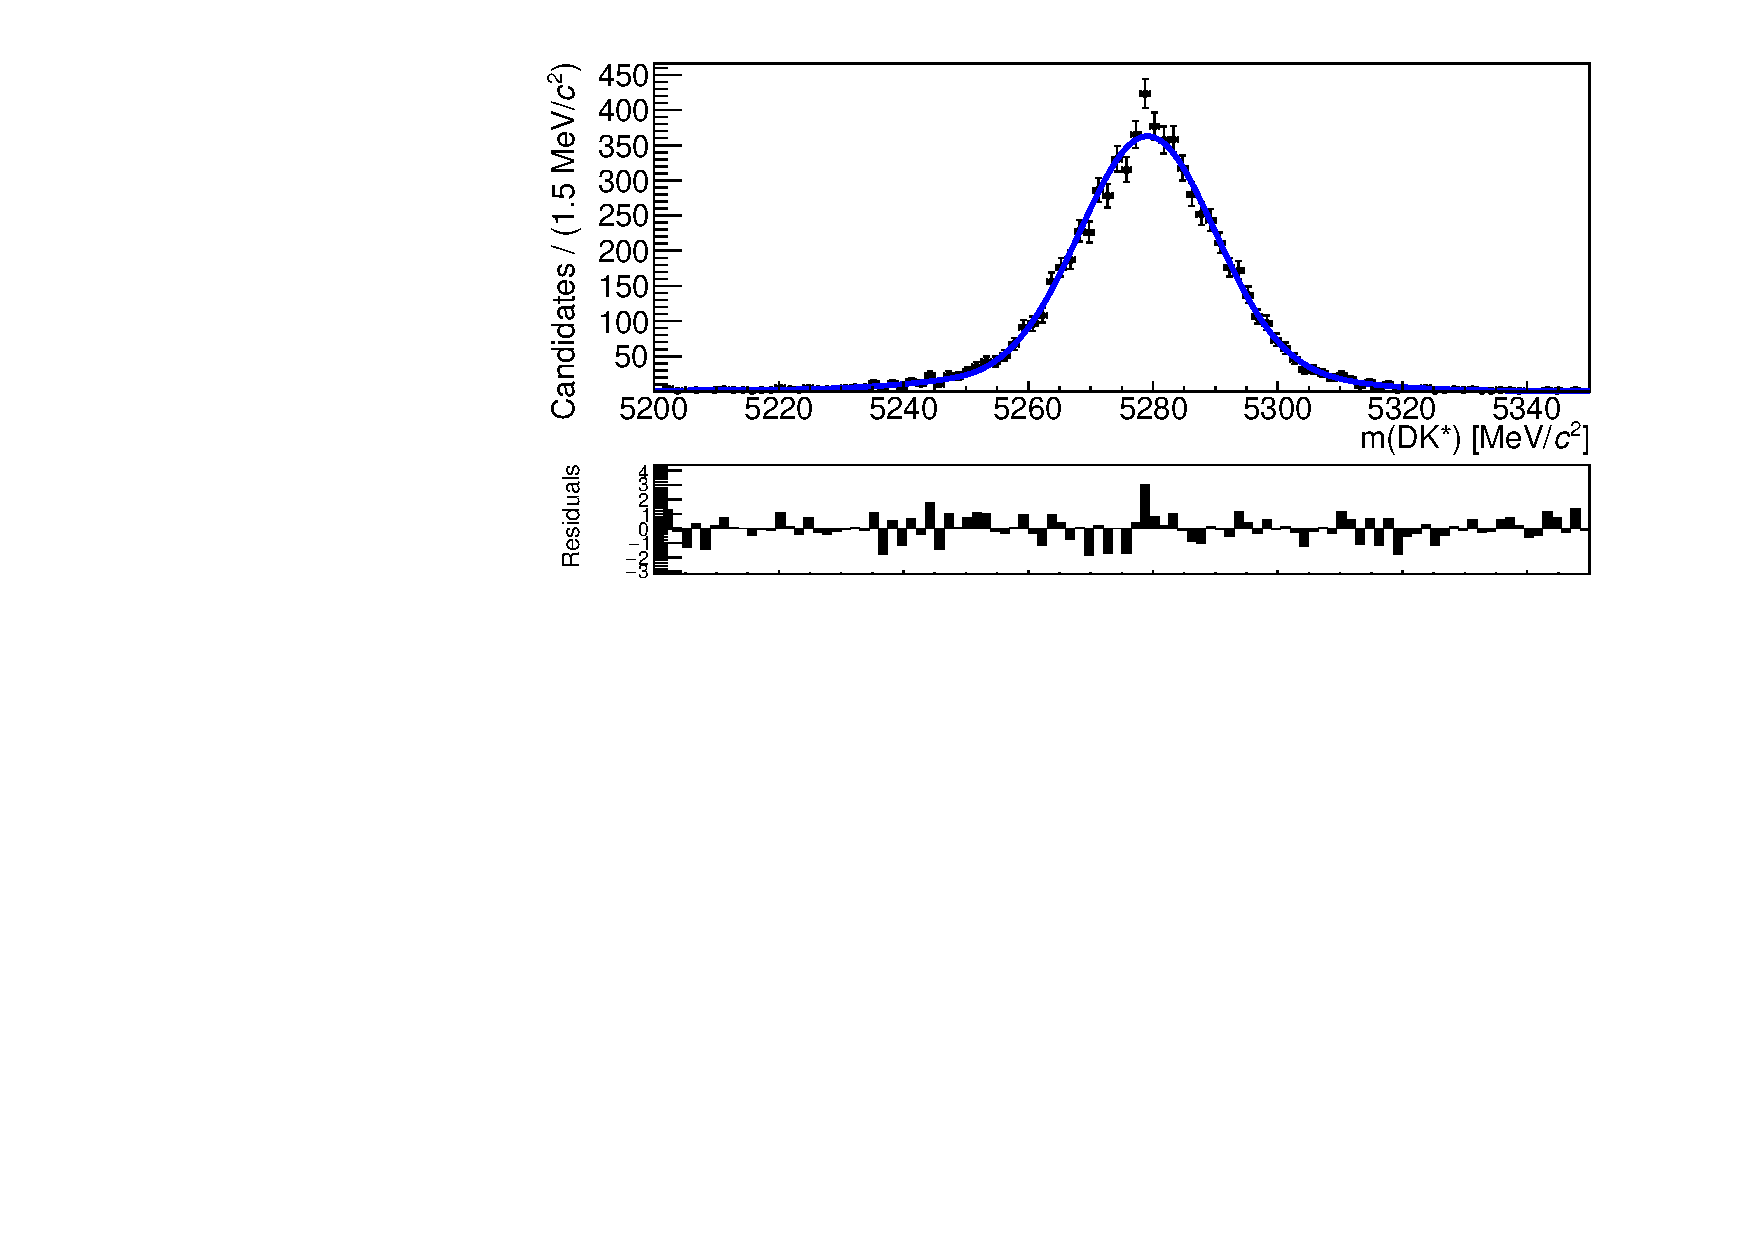
\includegraphics[width=0.5\linewidth]{figures/fitComponents/signalShape_LL_KPi.pdf}
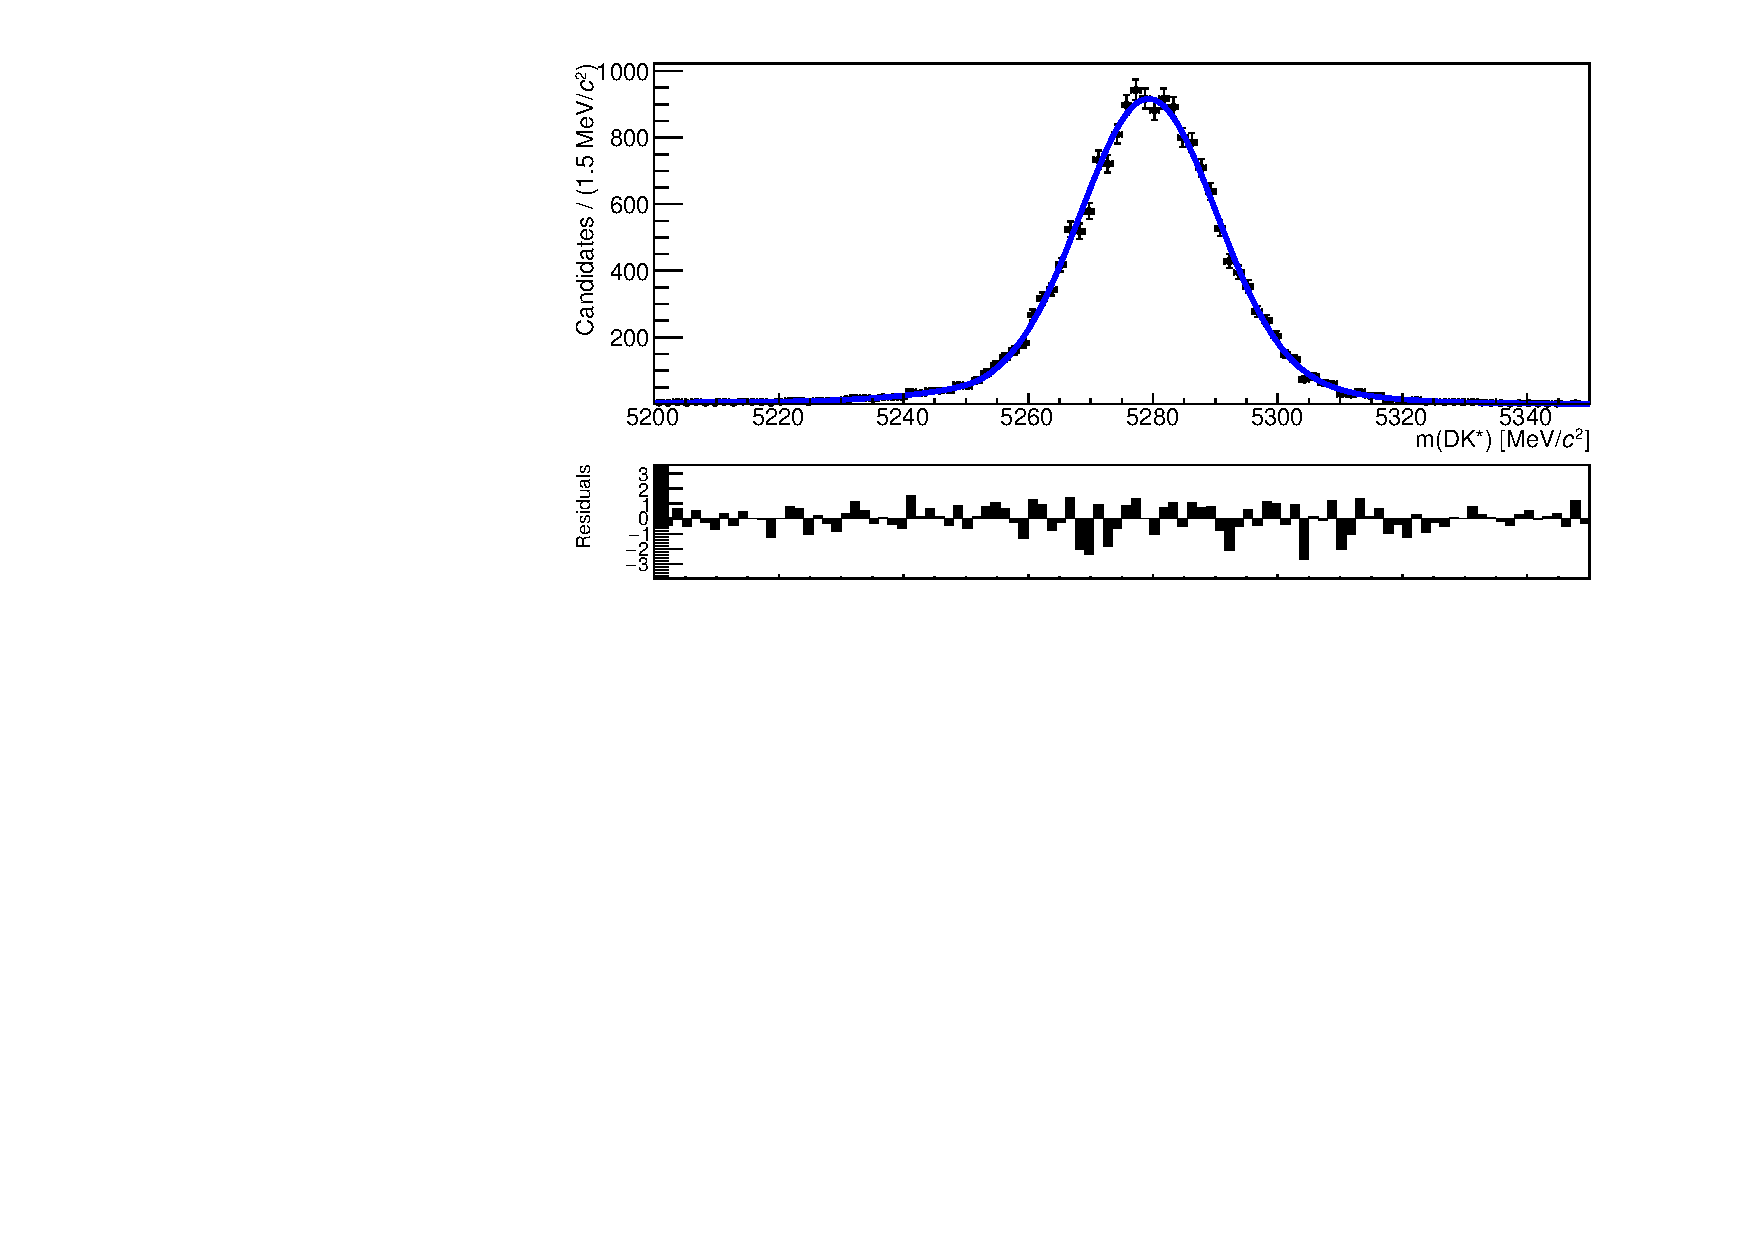
\includegraphics[width=0.5\linewidth]{figures/fitComponents/signalShape_DD_KPi.pdf}
\put(-390,70) {(a)}
\put(-180,70) {(b)}
\hfill
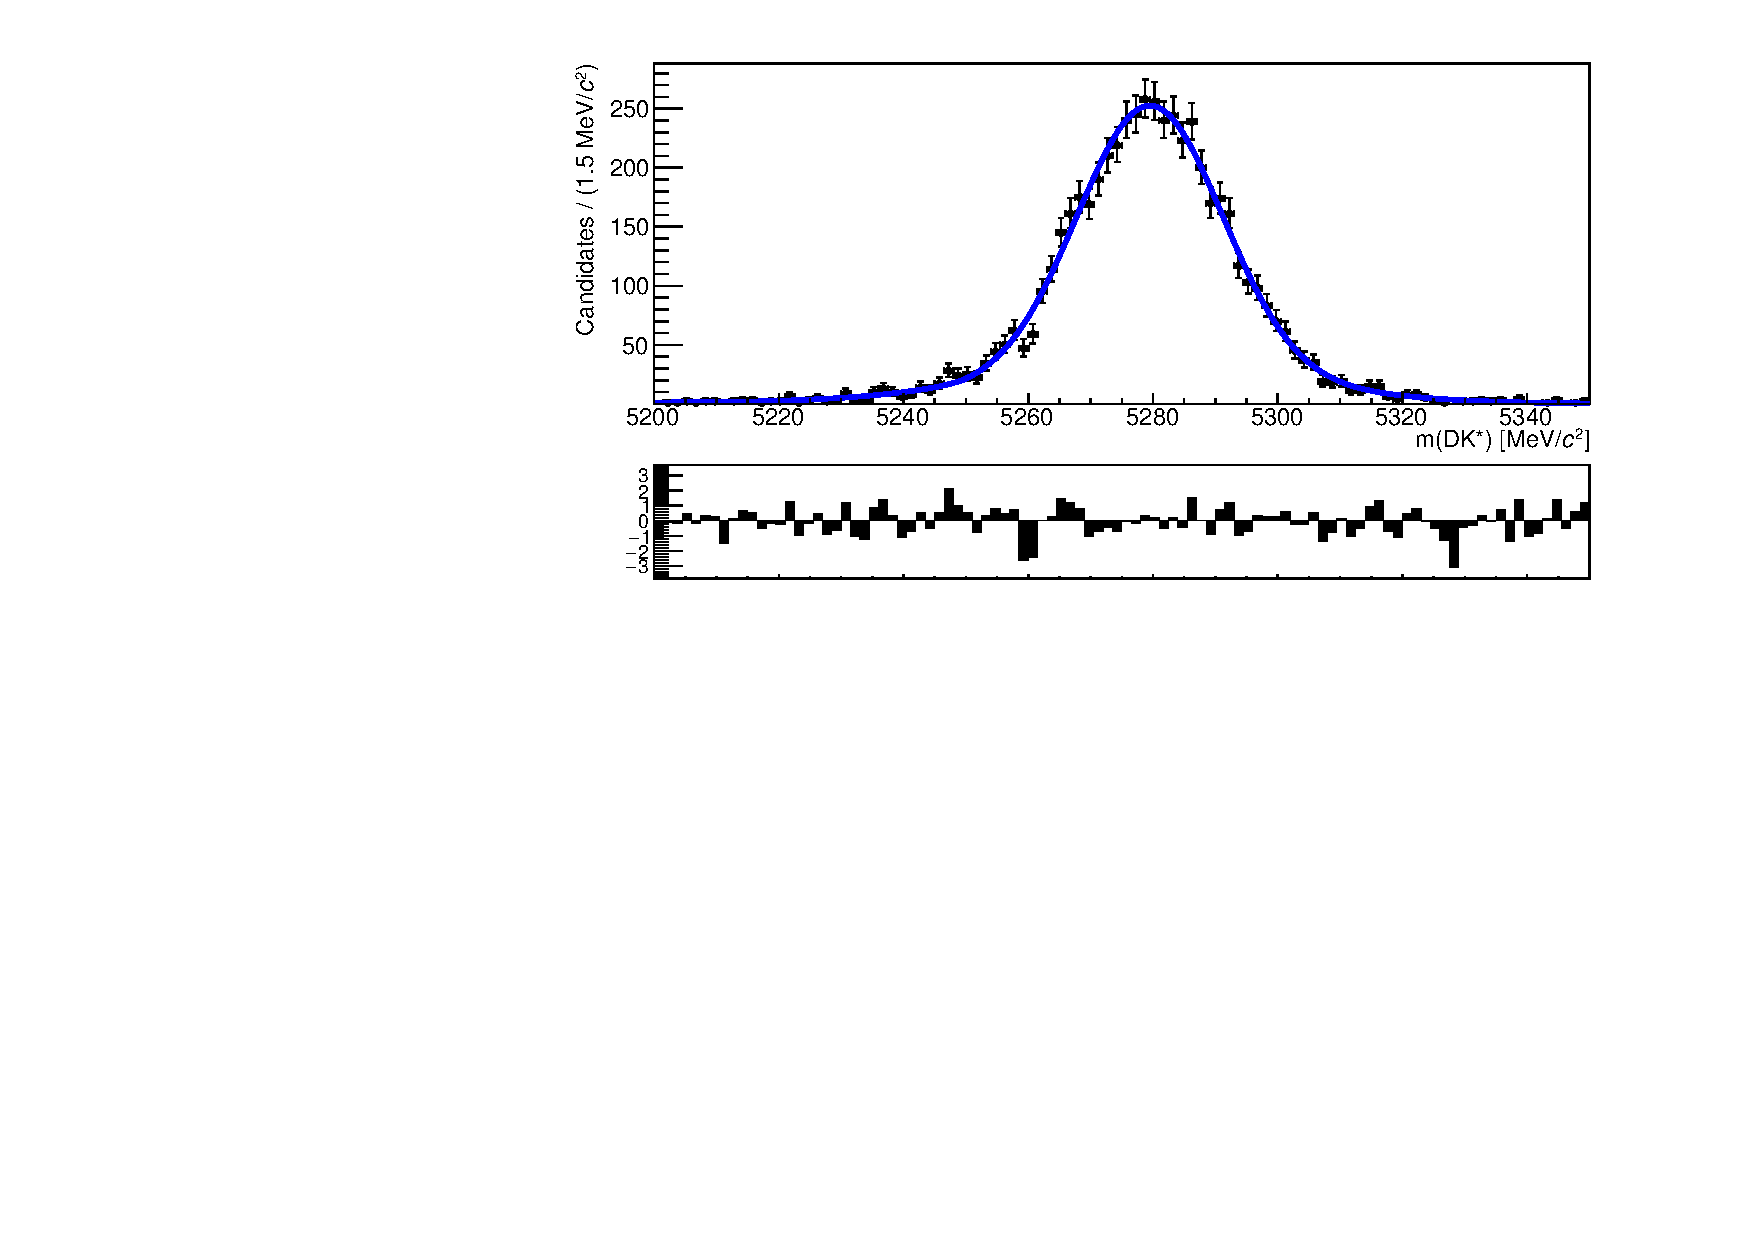
\includegraphics[width=0.5\linewidth]{figures/fitComponents/signalShape_LL_KPiPiPi.pdf}
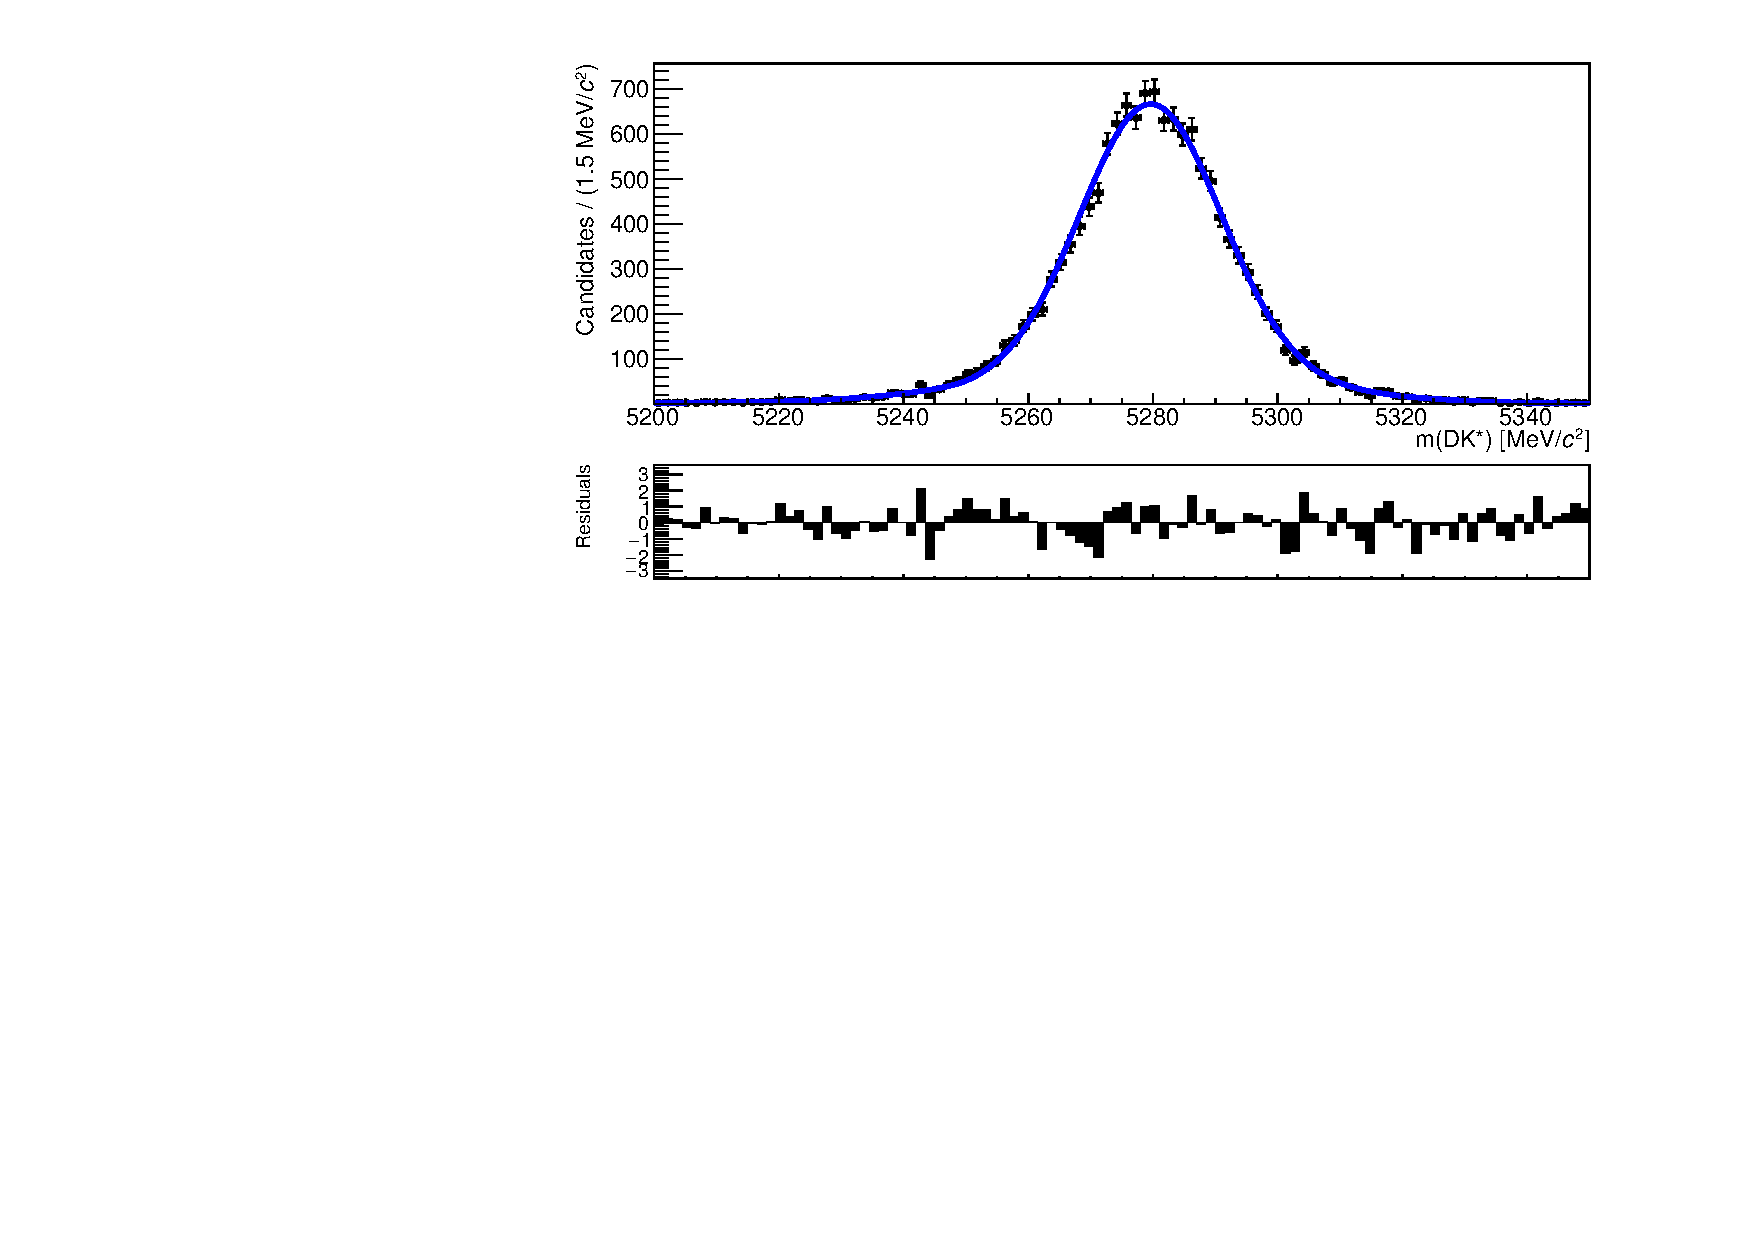
\includegraphics[width=0.5\linewidth]{figures/fitComponents/signalShape_DD_KPiPiPi.pdf}
\put(-390,70) {(c)}
\put(-180,70) {(d)}
\caption{Fits to \runone and \runtwo simulated signal samples combined for (a) $K\pi$ LL, (b) $K\pi$ DD, (c) $K\pi\pi\pi$ LL, and (d) $K\pi\pi\pi$ DD}
\label{signalfits}
\end{figure}

\begin{table}[h]
\centering
\begin{tabular}{c|cc|cc}
\hline
& \multicolumn{2}{c}{$K\pi$} & \multicolumn{2}{c}{$K\pi\pi\pi$} \\
& LL & DD & LL & DD\\
\hline
$\mu$ & $5279.12 \pm 0.15$ & $5279.30 \pm 0.09$ & $5279.62 \pm 0.12$ & $5279.50 \pm 0.19$ \\
$\sigma$ & $10.7 \pm 0.3$ & $10.8 \pm 0.2$ & $11.2 \pm 0.2$ & $11.6 \pm 0.3$ \\
$f_{\sigma}$ & $2.04 \pm 0.10$ & $1.97 \pm 0.06$ & $2.08 \pm 0.07$ & $2.10 \pm 0.11$ \\
$\alpha$ & $2.53 \pm 0.07$ & $2.46 \pm 0.04$ & $2.60 \pm 0.07$ & $2.50 \pm 0.10$ \\
$n$ & 1.0 (fixed) & 1.0 (fixed) & 1.0 (fixed) & 1.0 (fixed) \\
$f_{cb}$ & $0.82 \pm 0.03$ & $0.84 \pm 0.02$ & $0.80 \pm 0.03$ & $0.81 \pm 0.04	$ \\
\hline
\end{tabular}
\caption{Signal shape parameters obtained by a fit to \runone and \runtwo simulated signal samples combined for both $K\pi$ and $K\pi\pi\pi$. Parameter names are defined in Equation \ref{DCBshape}. All parameters except for the mean and width are fixed to these values in the mass fit}
\label{signalparameters}
\end{table}


\subsection{Combinatorial background}
\label{sec:massfit:combinatorial}

The combinatoric background comes from, for example, random tracks incorrectly reconstructed to form a \D meson. The combinatoric background is modelled using an exponential function with a freely floating slope parameter and yield. The slope parameter is allowed to float independently in the LL and DD categories and between two and four-body \D final states. Each \D final state can have a different combinatoric rate.


%%%%%%%%%%%%%%%%%%%%%%
\subsection{Partially reconstructed backgrounds}
\label{sec:massfit:partreco}

Partially reconstructed decays refer to those in which one or more particle has failed to be reconstructed. These decays are parameterised by analytic functions based on a previous studies of \decay{\Bm}{\D\Km}, \decay{\D}{h^+h^-} data~\cite{LHCb-PAPER-2016-003} and \decay{\Bz}{\D\Kstarz}, \decay{\D}{h^+h^-} data~\cite{LHCb-PAPER-2016-006}, which have many similar aspects to this analysis.

The partially reconstructed decays are of the form \decay{\B}{\Dstar\Kstar}, where the \Dstar decays to a \D meson and a pion or photon that is missed in reconstruction. These backgrounds are observed at a low reconstructed invariant mass due to the single particle missed from the invariant mass sum. The \B mass range is no large enough to include the case where more than one particle is lost. Three partially reconstructed decays contribute in the invariant mass fit:

\begin{itemize}
\item{\decay{\Bm}{(\decay{\Dstarz}{\Dz[\piz]})\Kstarm}}
\item{\decay{\Bm}{(\decay{\Dstarz}{\Dz[\gamma]})\Kstarm}}
\item{\decay{\Bd}{(\decay{\Dstarp}{\Dz[\pip]})\Kstarm}}
\end{itemize}

where the particle in square brackets corresponds to the missing daughter. All of the decay modes listed are modelled using three analytic shapes; RooHORNSdini, RooHILLdini and RooLITTLEHORNSdini, developed by Paolo Gandini and Faye Cheung. These shapes are physically motivated, exploiting the decay kinematics of partially reconstructed decays.

\decay{\B}{\Dstar\Kstar} is a Scalar $\to$ Vector Vector decay, therefore there are three different helicity amplitudes to consider due to the conservation of angular momentum. Each of these helicity amplitudes produces a \Dstar particle in a different helicity state, labelled +1, 0, -1. The helicity state of the \Dstar and the spin of the missing particle in the subsequent \Dstar decay determines the distribution of the reconstructed \B mass. 

\subsubsection{Horns function}

Consider the \decay{\Bm}{\Dstarz\Kstarm}, \decay{\Dstarz}{\Dz\piz}, where the \Dstarz is in helicity state 0. The helicity of the \Dstarz and the conservation of angular momentum mean that the spin-0 \piz meson will decay predominantly along $\theta = 0^{\circ}$ or $\theta = 180^{\circ}$. When $\theta = 0^{\circ}$, the fraction of momentum carried by the \piz in the \B rest frame is at its smallest, resulting in a larger reconstructed \B mass. Conversely, if $\theta = 180^{\circ}$, the fraction of momentum carried by the \piz is greatest, leading to a lower resonstructed \B mass. The distribution of the helicity angle of the missing particle, $\theta$, has a one-to-one correspondence with its momentum and therefore the reconstructed \B mass. This gives rise to a double peak structure. The \B mass distribution is a parabola, $p_{HORNS}(x)$, with kinematics endpoints $a$ and $b$ where

\begin{align}
p_{HORNS}(x) &= \begin{cases}
\left(x - \frac{a+b}{2}\right)^2, & \text{ if $a \leq x \leq b$}\\ 	
0, & \text{ otherwise.}
\end{cases} 
\end{align}

The parabola is convolved with two Gaussians in order to account for resolution effects. Given a Gaussian function of mean $\mu$ and width $\sigma$, $G(\mu,\sigma)$, a Double Gaussian can be constructed as,

\begin{equation}
DG(x) = f_G G(x|\mu,\sigma) + \left(1-f_G\right) G(x|\mu,R_{\sigma}\sigma) \text{ , }
\end{equation}

where $\sigma$ is the width of the first Gaussian, $f_G$ is the fraction contained by the first gaussian and $R_{\sigma}$ is the relative width between the two. Additionally, selection effects can affect the shape such that one peak is higher than the other. This is taken into account by introducing a linear polynomial with a slope of $1 - \xi$, where $0 \leq \xi \leq 1$. As $\xi \rightarrow 0$, the left hand peak decreases in size relative to the right hand peak. The resulting Horns function is,

\begin{equation}
\text{Horns}(m) = \int_a^b dx \left(x - \frac{a+b}{2}\right)^2 DG(x|m,\sigma,f_G,R_{\sigma}) \left( \frac{1 - \xi_{HORNS}}{b - a}x + \frac{b\xi_{HORNS} - a}{b - a}\right),
\label{eqn:horns}
\end{equation}

where $m$ is the mass variables to be fitted and $x$ is the integration variable in the convolution.

\subsubsection{Hill function}

Consider the \decay{\Bm}{\Dstarz\Kstarm}, \decay{\Dstarz}{\Dz\gamma}, where the \Dstarz is in helicity state 0. The helicity of the \Dstarz and the conservation of angular momentum mean that the spin-1 \Pgamma will decay predominantly along $\theta = 90^{\circ}$ or $\theta = 270^{\circ}$. The fraction of momentum carried by the photon is the same in both of these cases, so not double peak stucture is seen. The resultsing \B mass distribution is a parabola with negative curvature, $p_{HILL}(x)$, and kinematic endpoints $a$ and $b$ where

\begin{align}
p_{HILL}(x) &= \begin{cases}
-(x - a)(x - b), & \text{ if $a \leq x \leq b$}\\ 	
0, & \text{ otherwise.}
\end{cases} 
\end{align}

As with the Horns function, this parabola is convolved with a Double Gaussian and a linear polynomial to account for resolution and selection effects respectively. The resultsing Hill function is,

\begin{equation}
\text{Hill}(m) = \int_a^b dx \left[-(x - a)(x - b)\right] DG(x|m,\sigma,f_G,R_{\sigma}) \left( \frac{1 - \xi_{HILL}}{b - a}x + \frac{b\xi_{HILL} - a}{b - a}\right),
\label{eqn:hill}
\end{equation}

where $m$ is the mass variables to be fitted and $x$ is the integration variable in the convolution.

As the distribution of $\theta$ has a one-to-one correspondence with the reconstructed \B mass, a \Dstar of +1 or -1 would be indistiguishable in \B mass therefore these values are grouped together. This Hill function also applies to the \decay{\Bm}{\Dstarz\Kstarm}, \decay{\Dstarz}{\Dz\piz}, where the \Dstarz is in helicity state $\pm$1.

\subsubsection{Little Horns function}

For the configuration \decay{\Bm}{\Dstarz\Kstarm}, \decay{\Dstarz}{\Dz\gamma}, where the \Dstarz is in helicity state $\pm$1, a third shape is needed, named Little Horns. It is described by a parabola, $p_{LITTLEHORNS}(x)$, and kinematic endpoints $a$ and $b$ where

\begin{align}
p_{LITTLEHORNS}(x) &= \begin{cases}
\left(x - \frac{a+b}{2}\right)^2 + \left(\frac{a-b}{2}\right)^2, & \text{ if $a \leq x \leq b$}\\ 	
0, & \text{ otherwise.}
\end{cases} 
\end{align}

Again, this distribution is convolved with a Double Gaussian and linear polynomial to descibe the resolution and selection effects respectively. This results in a Little Horns function

\begin{multline}
\text{LittleHorns}(m) = \int_a^b dx \biggl\{ \left[ \left( x - \frac{a+b}{2} \right) ^2 + \left( \frac{a-b}{2} \right) ^2 \right] DG(x|m,\sigma,f_G,R_{\sigma}) \\
\left( \frac{1 - \xi_{LITTLEHORNS}}{b - a}x + \frac{b\xi_{LITTLEHORNS} - a}{b - a} \right) \biggr\}
\label{eqn:littlehorns}
\end{multline}

\subsubsection{Total partially reconstructed function}

Table \ref{helicityamplitudes} summarises the uses of the different analytic shapes described: Horns, Hill and Little Horns functions. In order to obtain values for the various parameters in these shapes simulated events were generated and the full reconstruction and selection was applied, except for the PID selection. Comparisons between \runone and \runtwo simulated events for partially reconstructed decays are shown in Figure \ref{parterecofits}. These distributions are considered sufficienctly similar to fix the shapes across all years. The parameters for the partially reconstructed shapes are obtained from performing individual fits to \runone simulated samples.

\begin{figure}[!h]
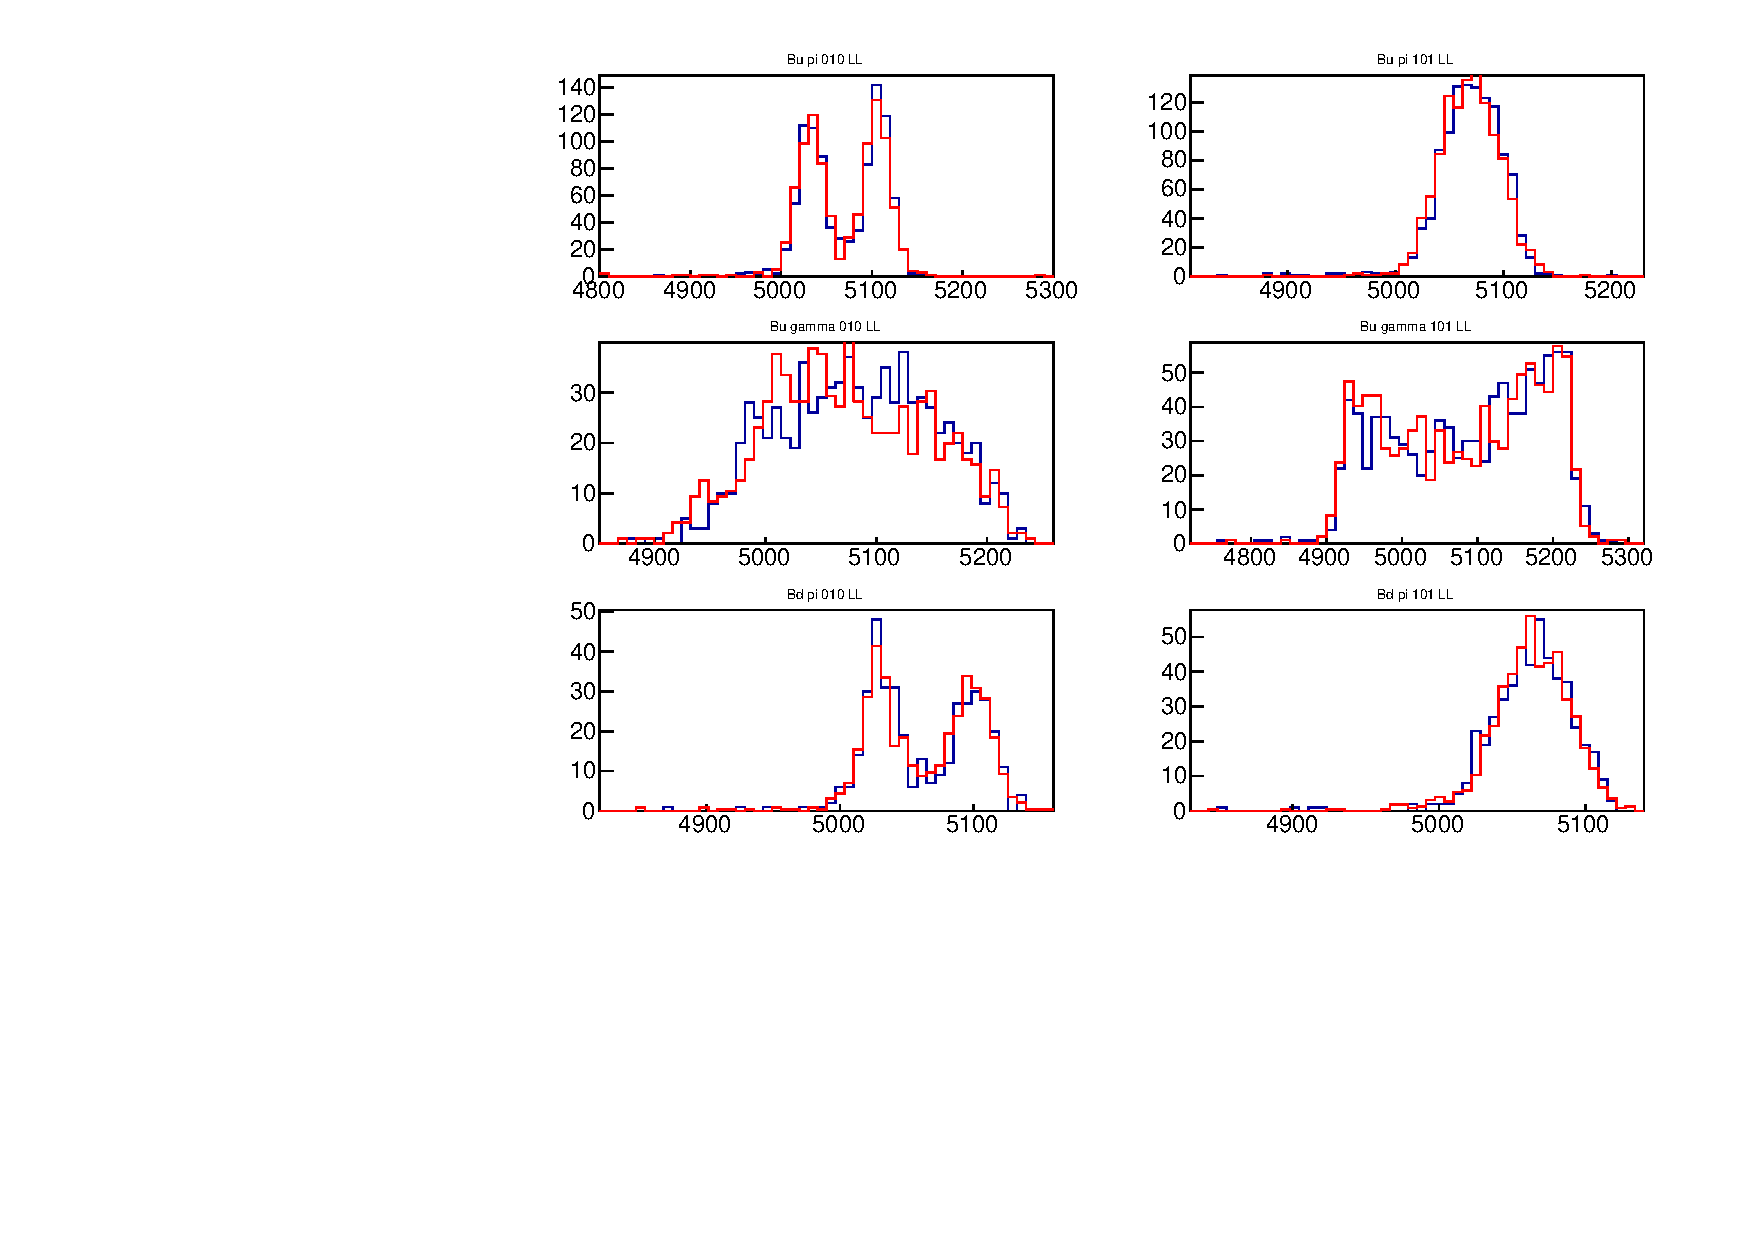
\includegraphics[width=\linewidth]{figures/compareMC/run1vsrun2MC_partreco_LL.pdf}
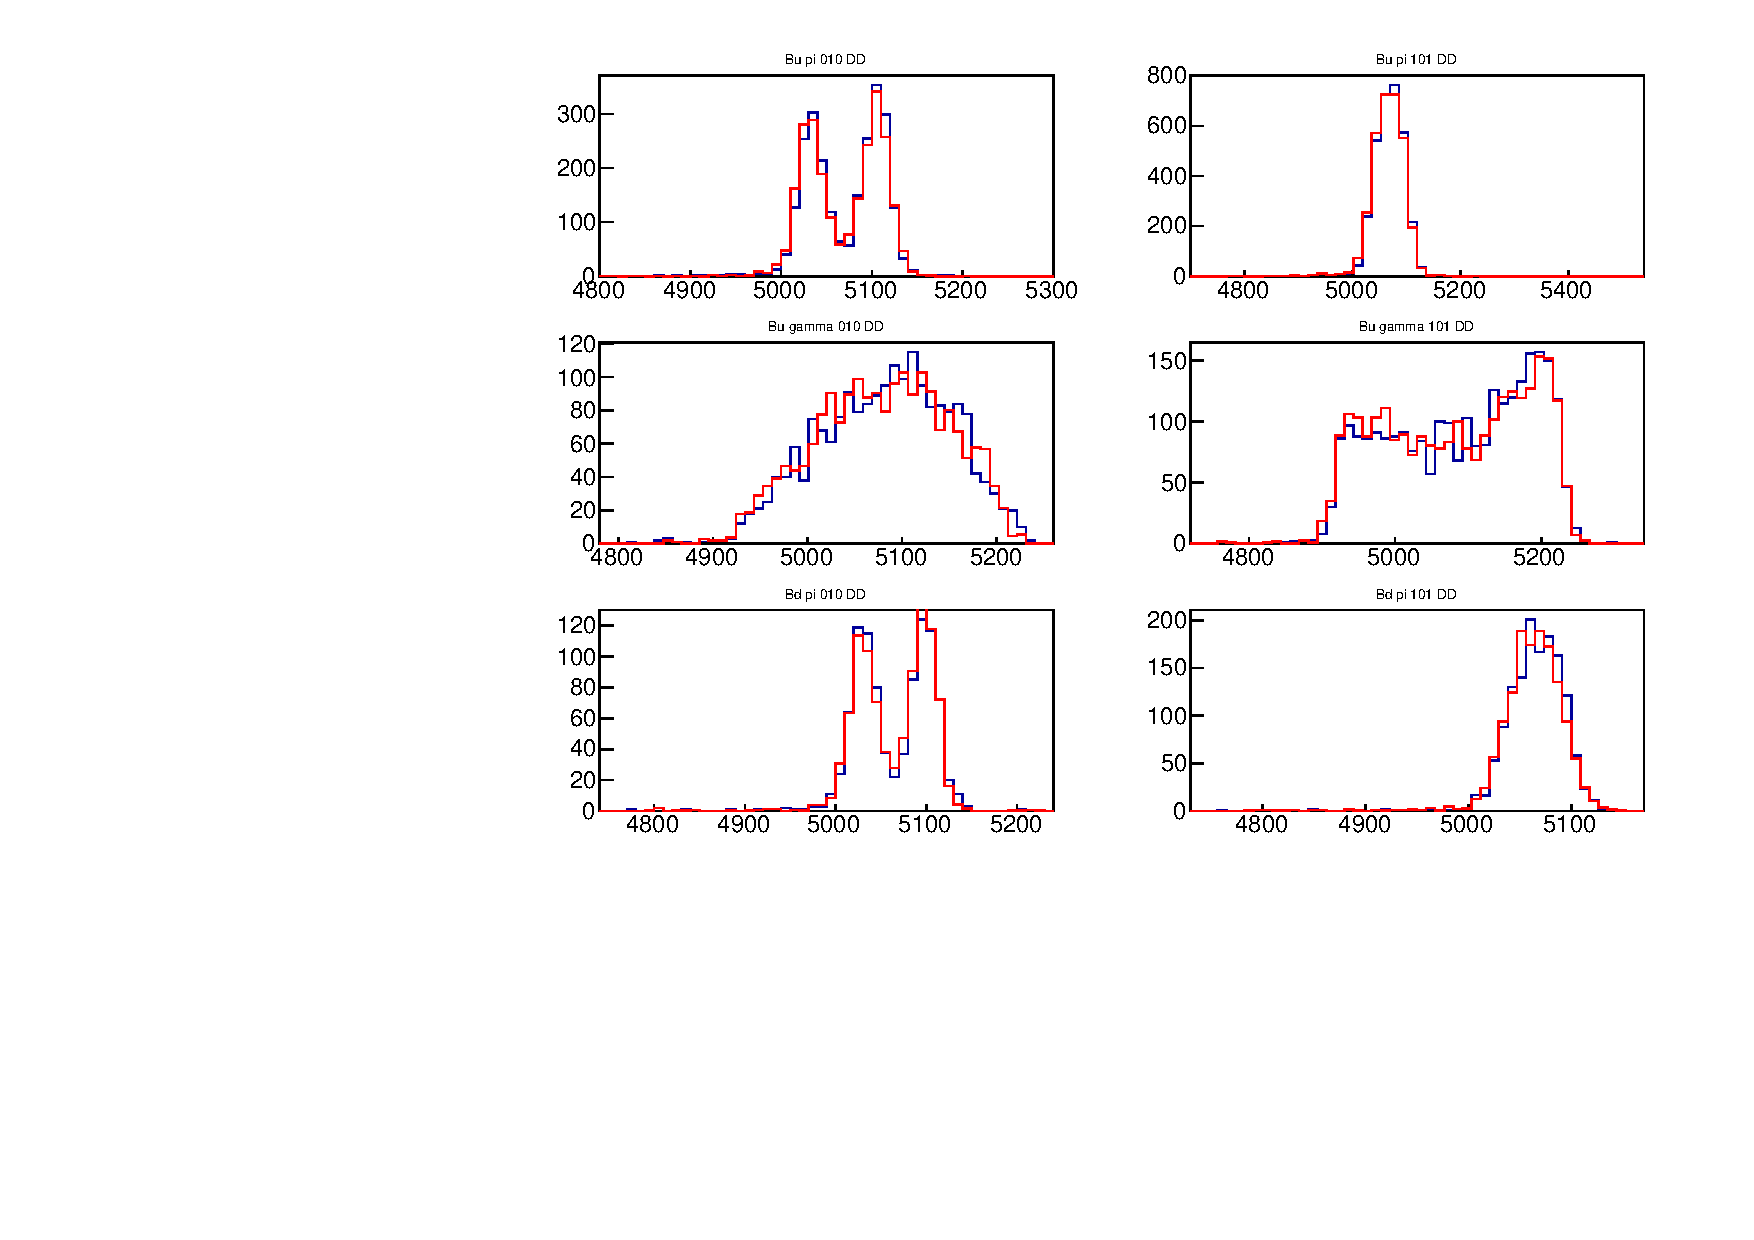
\includegraphics[width=\linewidth]{figures/compareMC/run1vsrun2MC_partreco_DD.pdf}
\caption{Comparison of partially reconstructed MC between Run 1 (blue) and 2015 (red). The different shapes correspond to different \Dstar\Kstar modes, descibed in Section \ref{sec:massfit:partreco}}
\label{parterecofits}
\end{figure}

The shapes are taken from simulation are fitted separately using the functions given by equations \ref{eqn:horns}, \ref{eqn:hill} and \ref{eqn:littlehorns}, the fits are shown in Figures \ref{partrecofitsLL} and \ref{partrecofitsDD}. All the parameters for these shapes are fixed in the mass fit from fits to simultated events. The values of these fixed parameters are given in Tables ?

\begin{table}[h]
\centering
\begin{tabular}{cccc}
Helicity of \Dstar & Missing particle & $\theta$ dependence & Function \\
\hline
0 & $\pi$ & $\left(x - \frac{a+b}{2}\right)^2$ & Horns, from Eq.~\ref{eqn:horns} \\
0 & \Pgamma & $-(x - a)(x - b)$ & Hill, from Eq.~\ref{eqn:hill} \\
$\pm$1 & $\pi$ & $-(x - a)(x - b)$ & Hill, from Eq.~\ref{eqn:hill} \\
$\pm$1 & \Pgamma & $\left(x - \frac{a+b}{2}\right)^2 + \left(\frac{a-b}{2}\right)^2$ & Little Horns, from Eq.~\ref{eqn:littlehorns} \\
\end{tabular}
\caption{Possible combinations of \Dstar helicity angle and missing particle and how this relates to the dependence on the helicity angle and the \B mass parameterisation}
\label{helicityamplitudes}
\end{table}

\begin{figure}[h]
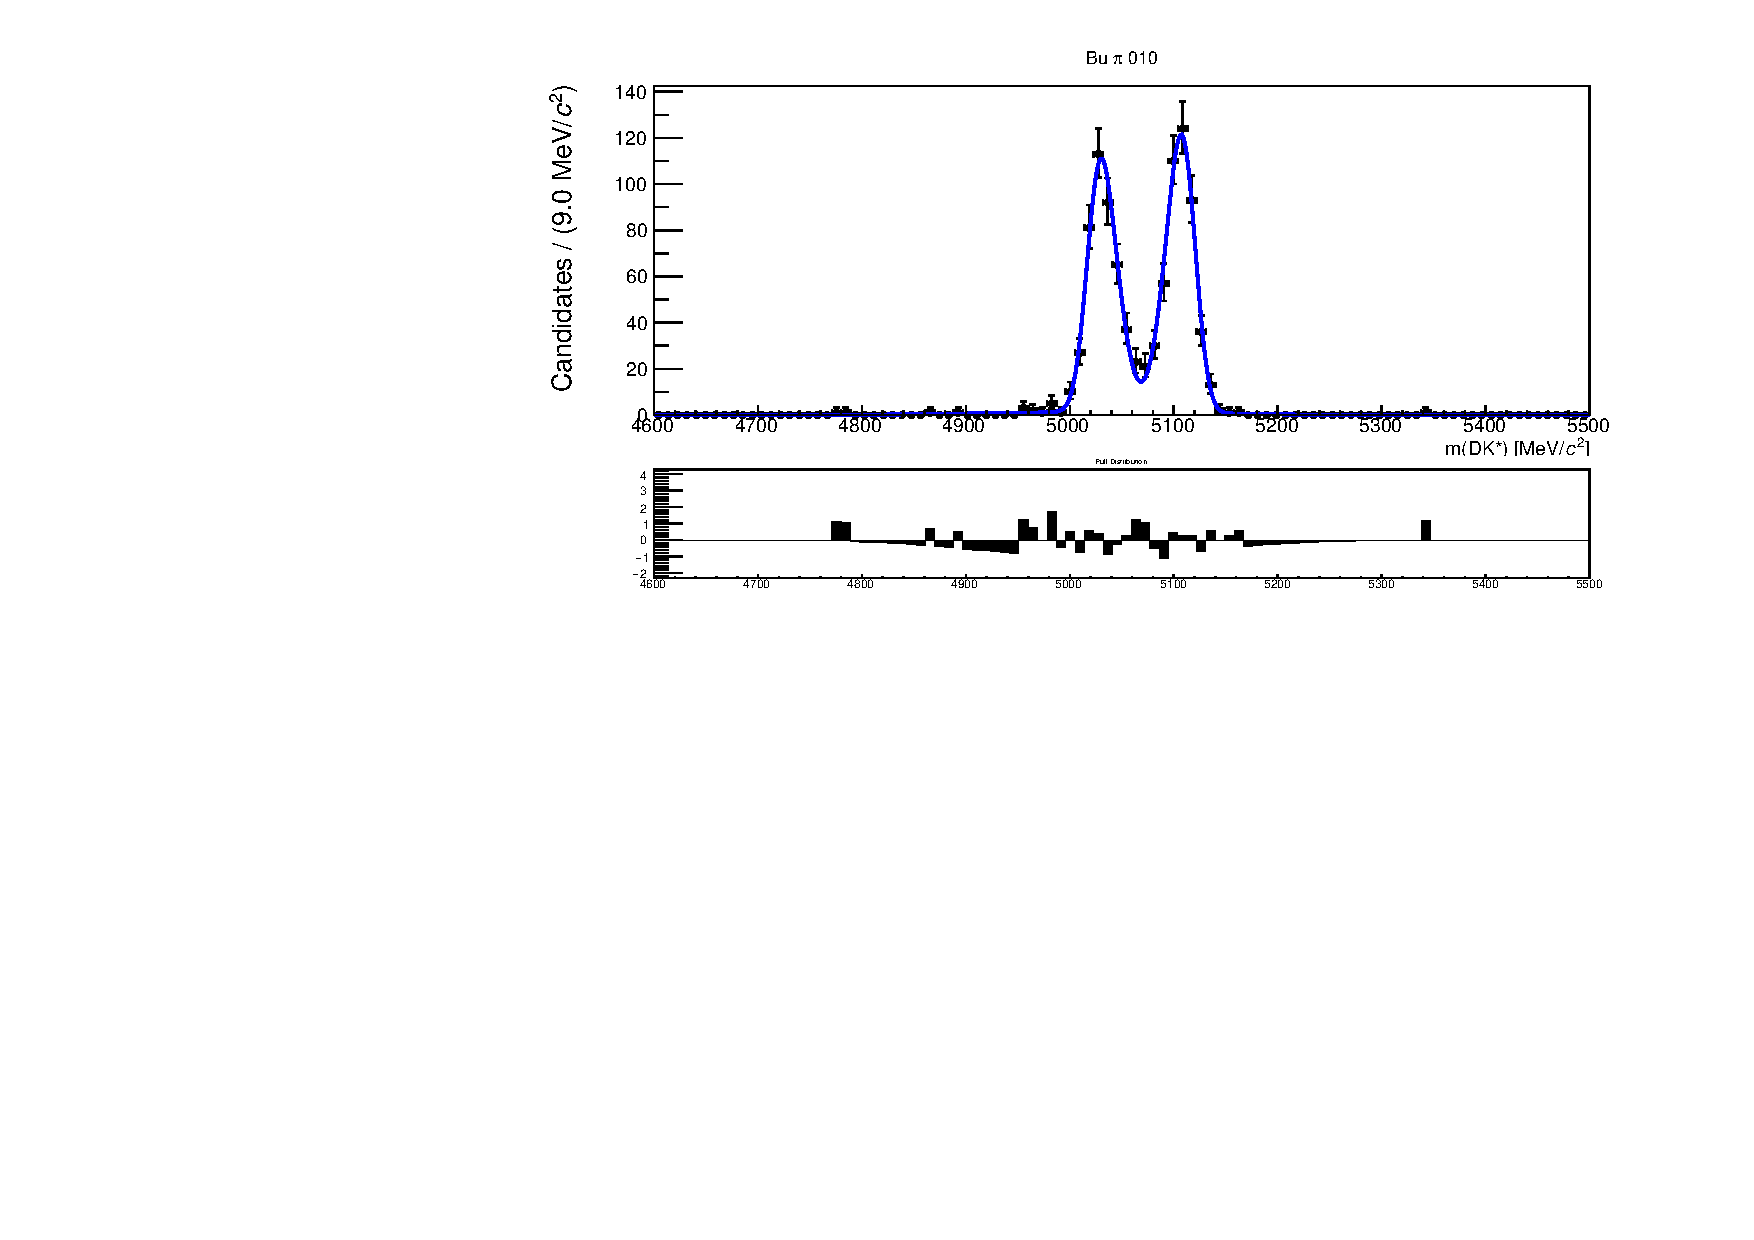
\includegraphics[width=0.5\linewidth]{figures/fitComponents/Bupi010_LL.pdf}
\put(-180,80) {(a)}
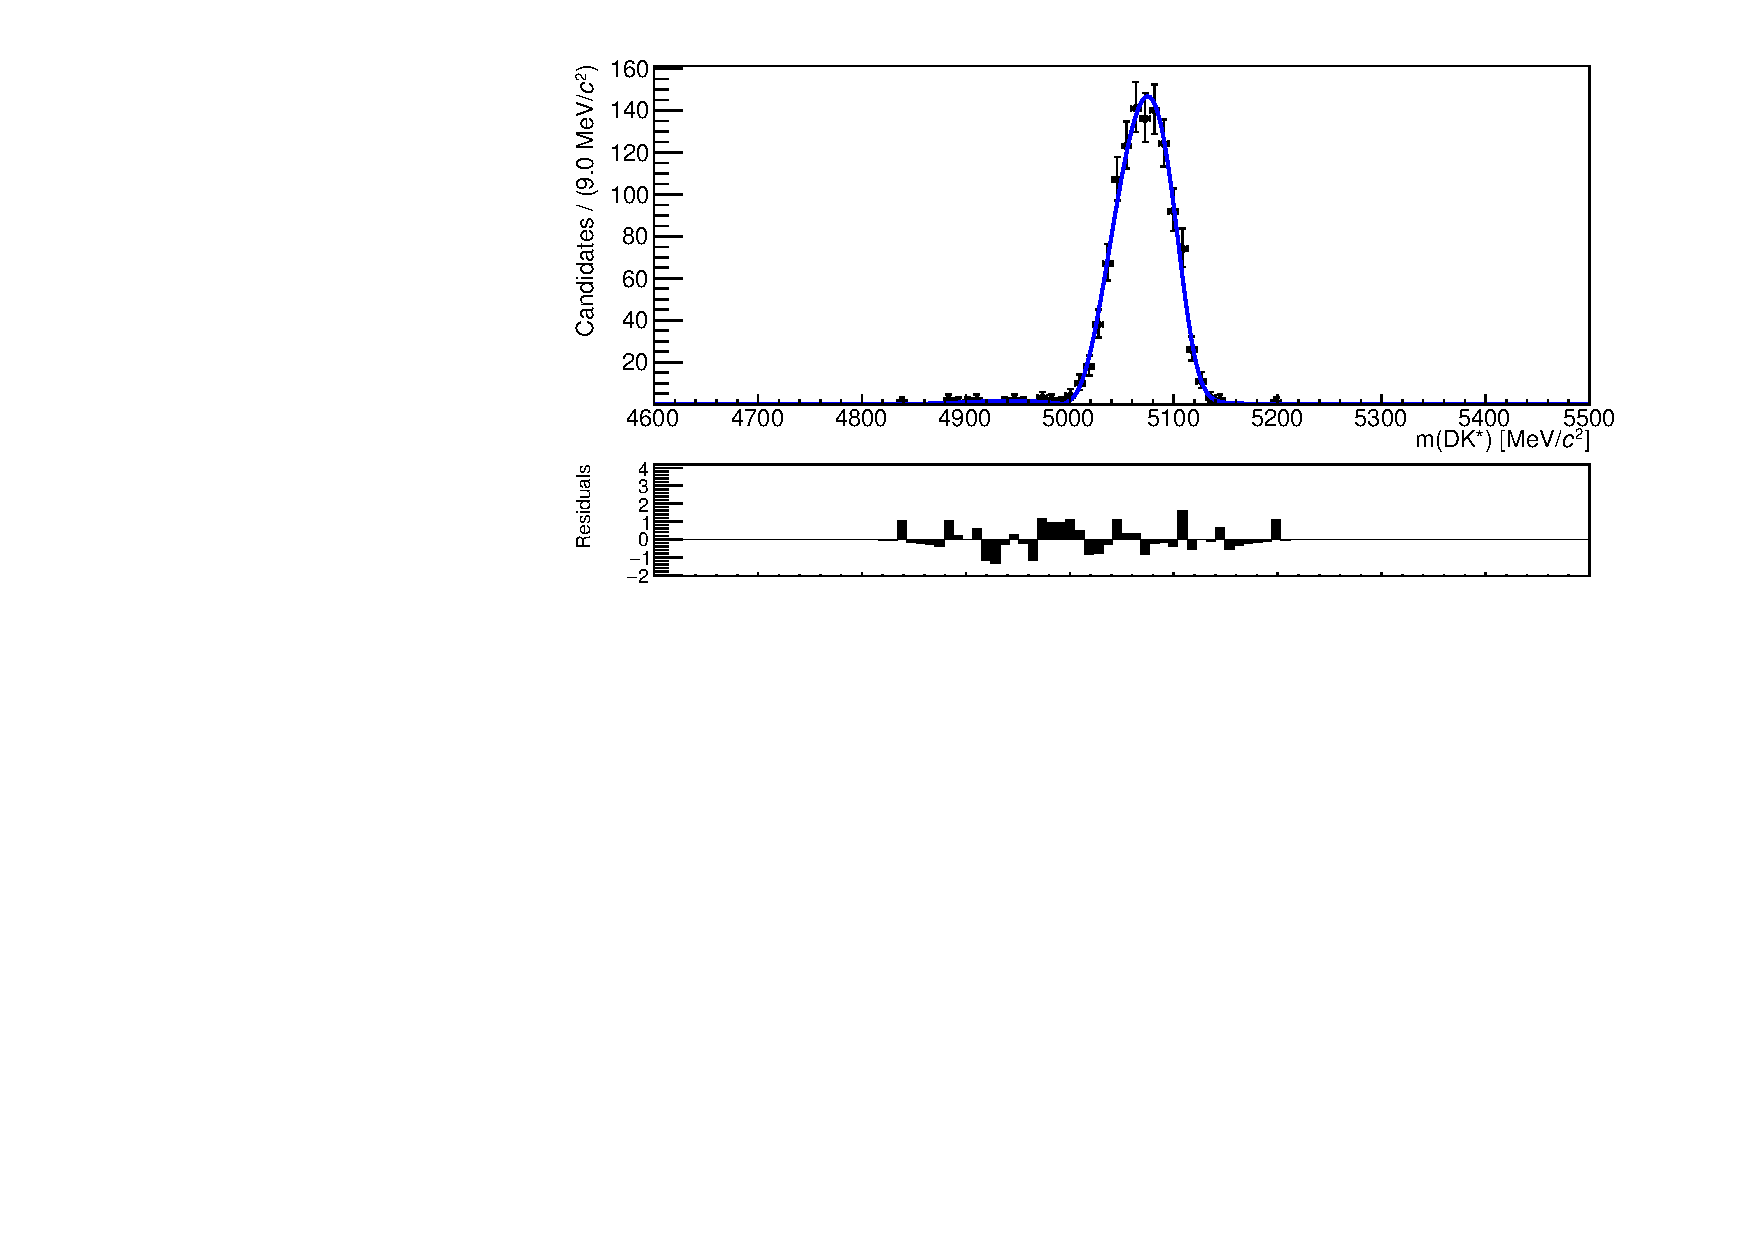
\includegraphics[width=0.5\linewidth]{figures/fitComponents/Bupi101_LL.pdf}
\put(-180,80) {(b)}
\hfill
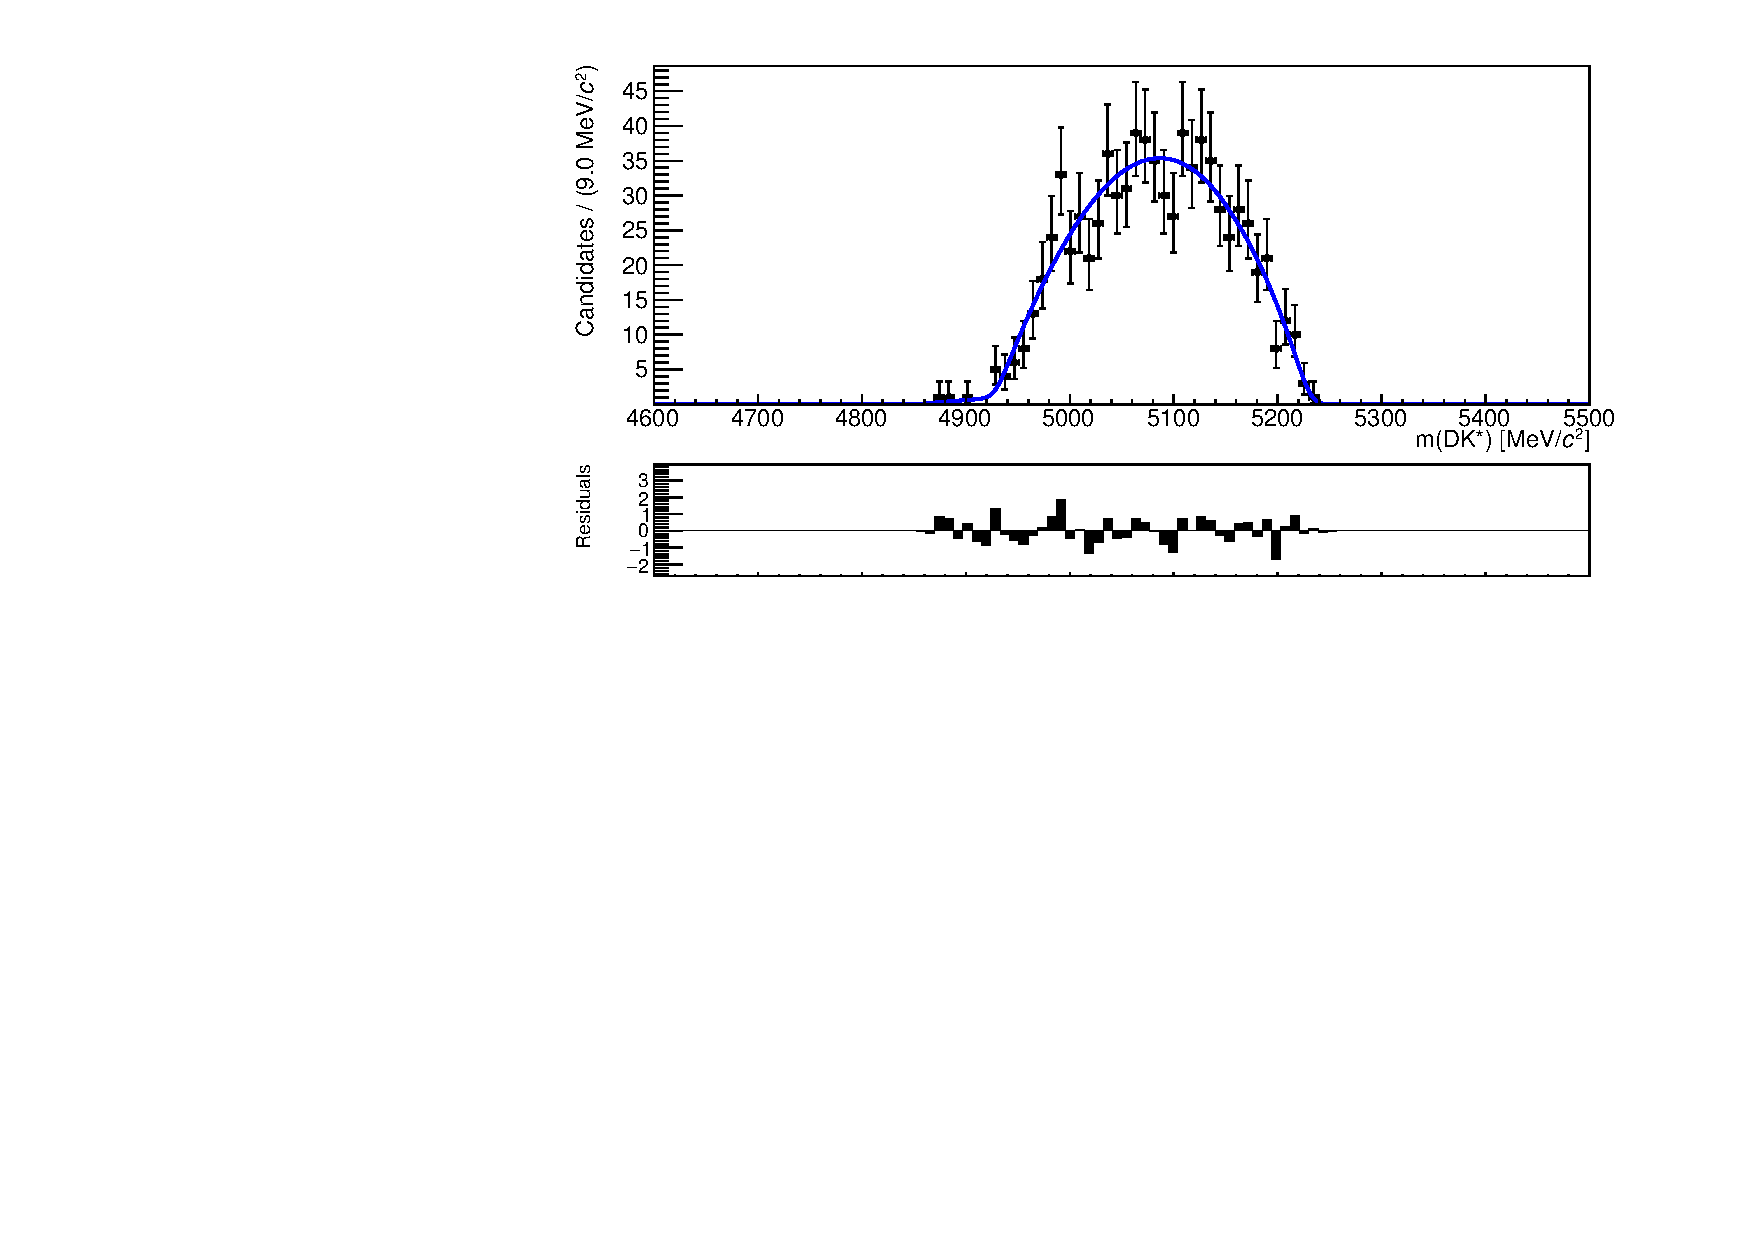
\includegraphics[width=0.5\linewidth]{figures/fitComponents/Bugamma010_LL.pdf}
\put(-180,80) {(c)}
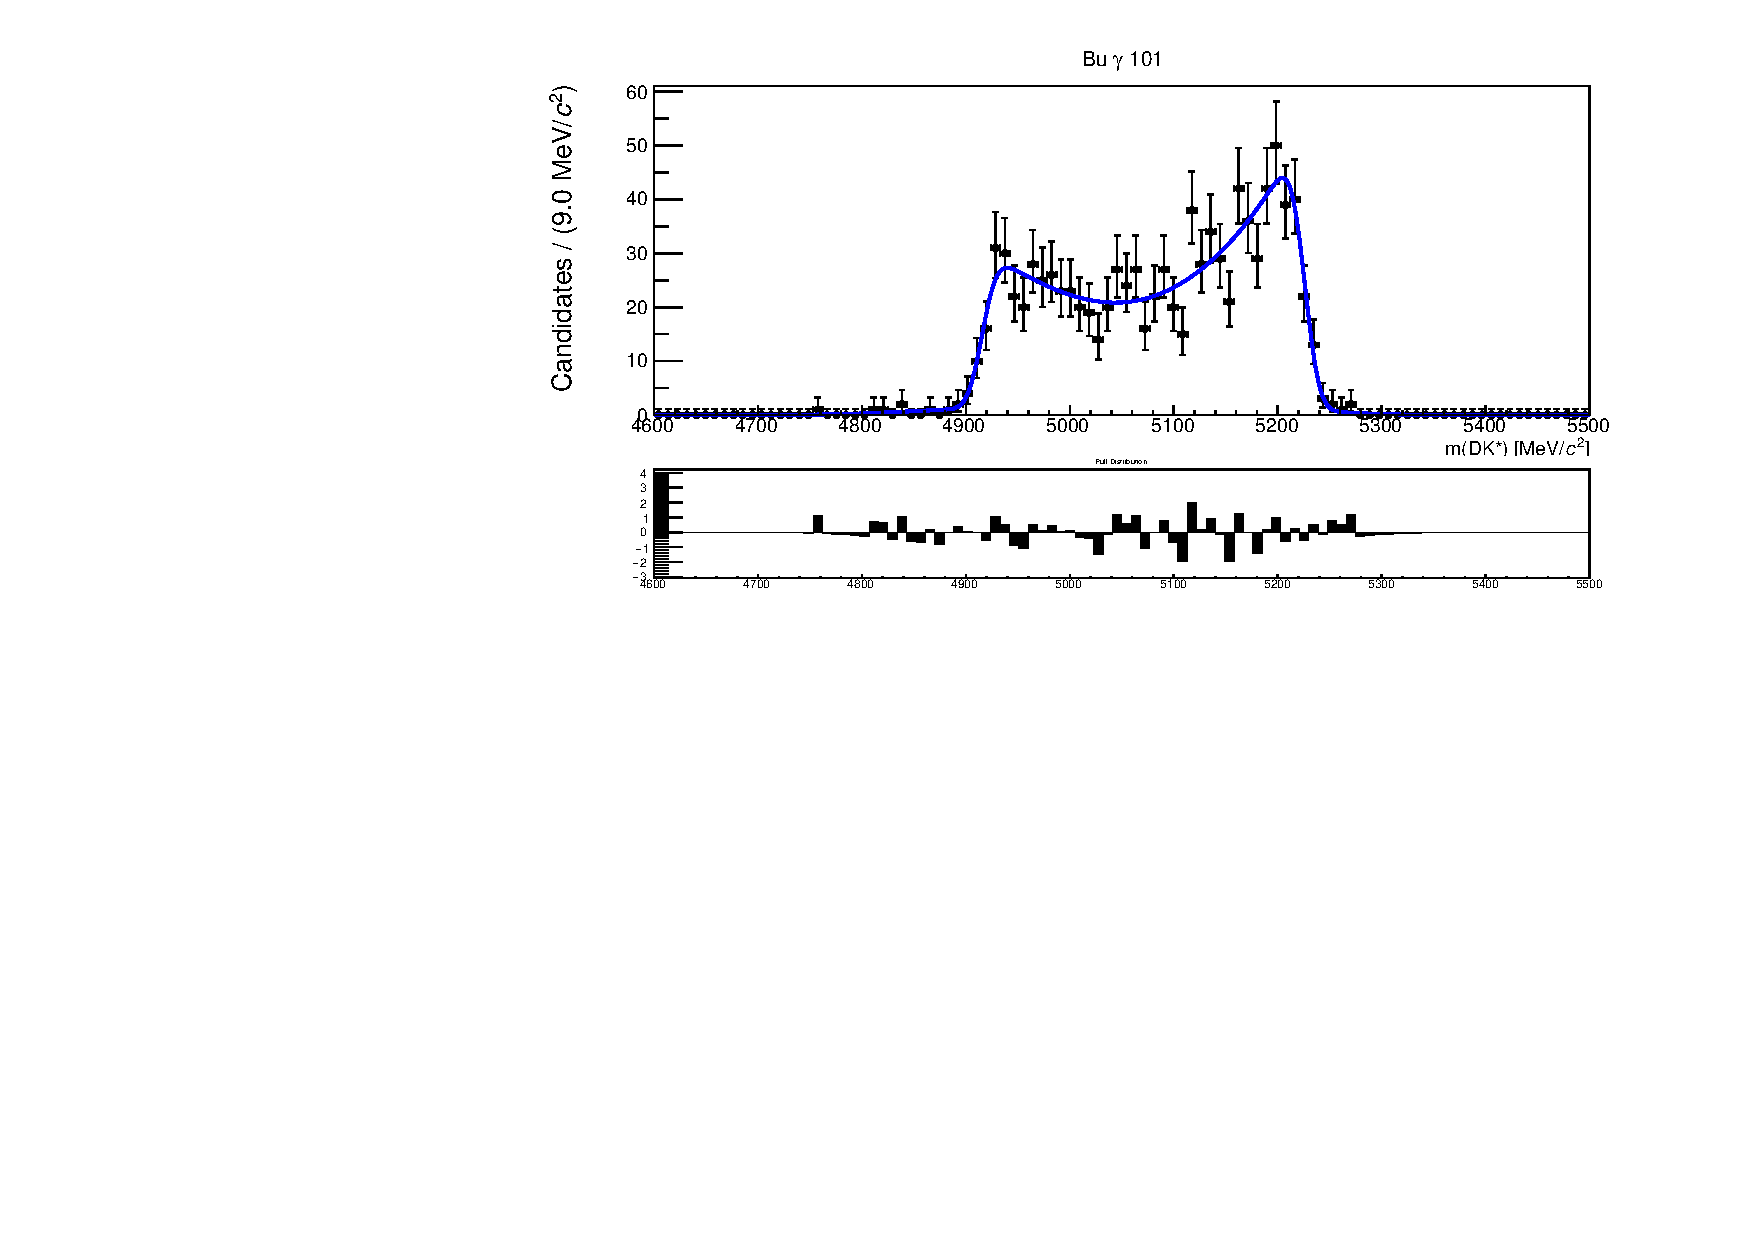
\includegraphics[width=0.5\linewidth]{figures/fitComponents/Bugamma101_LL.pdf}
\put(-180,80) {(d)}
\hfill
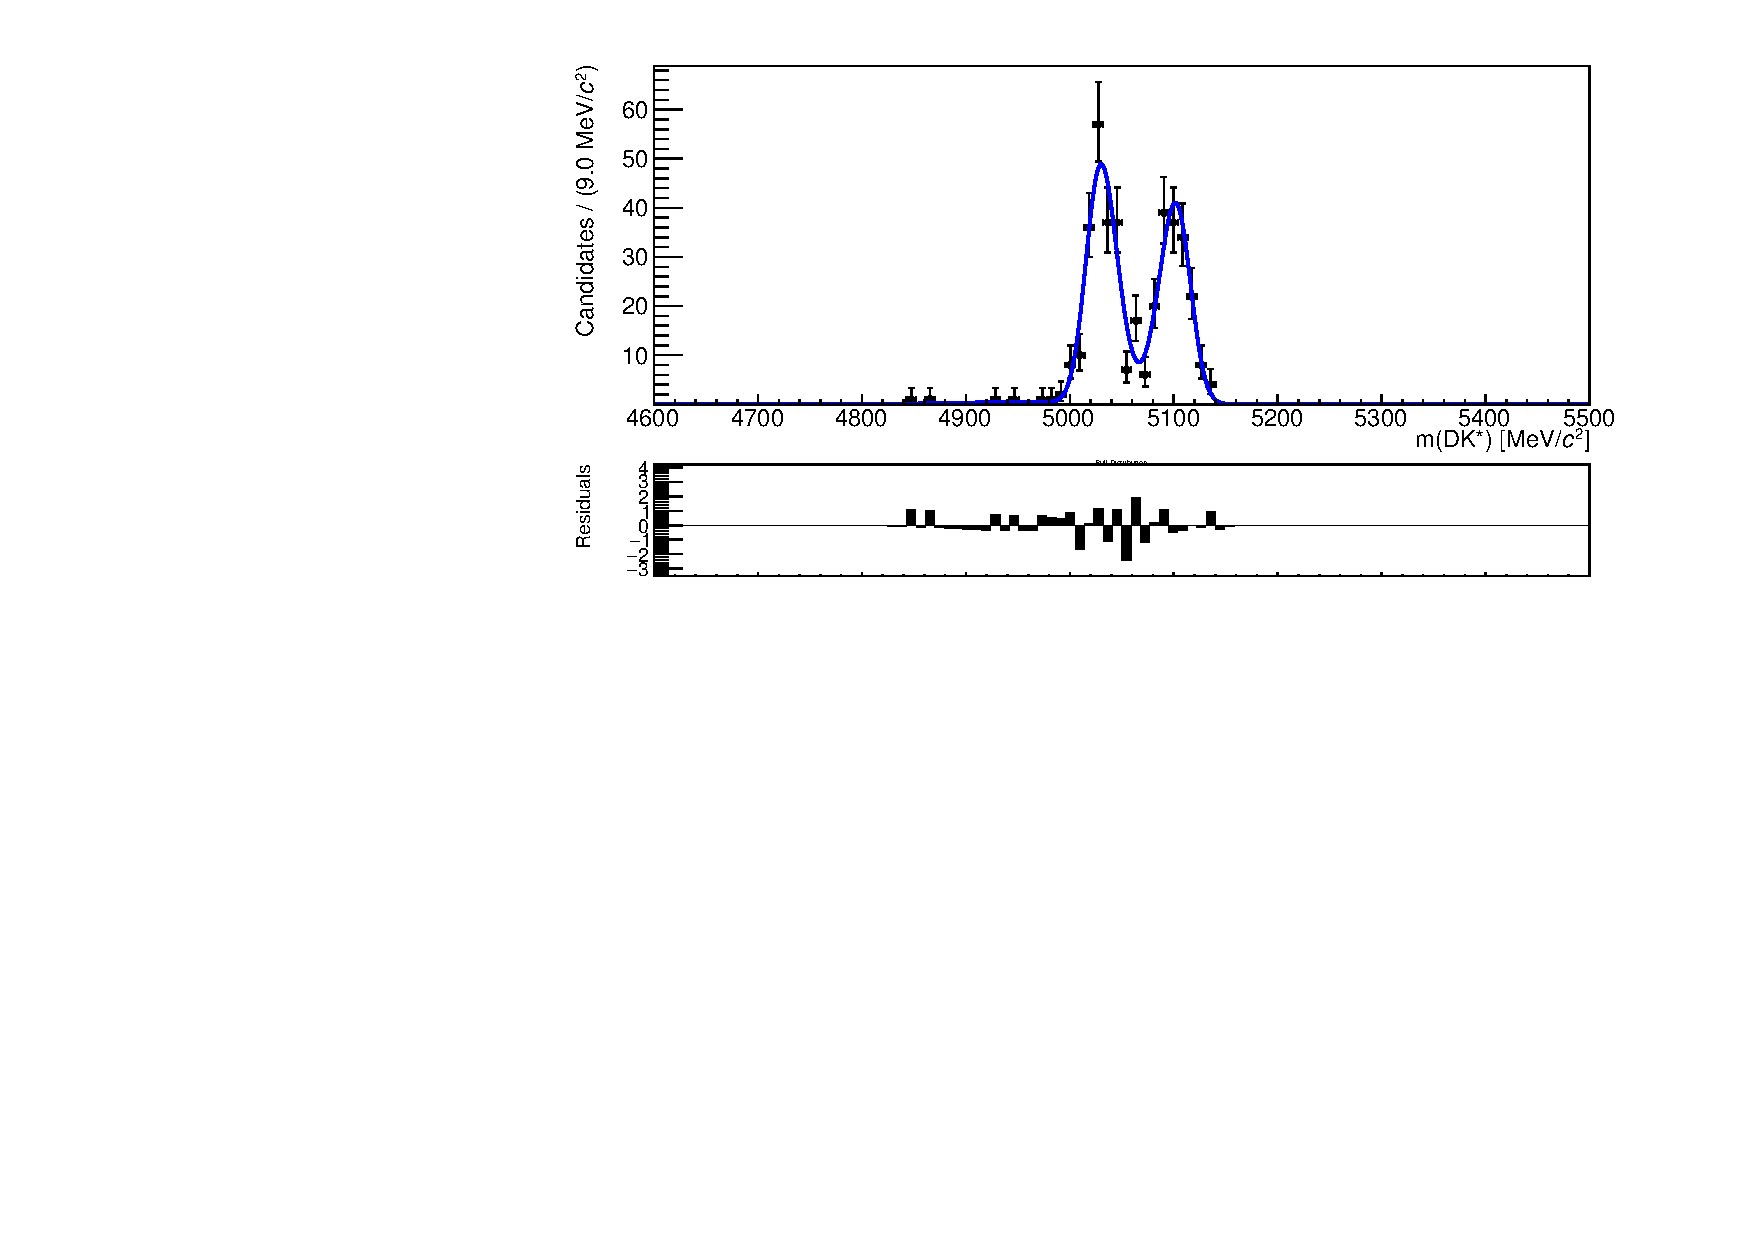
\includegraphics[width=0.5\linewidth]{figures/fitComponents/Bdpi010_LL.pdf}
\put(-180,80) {(e)}
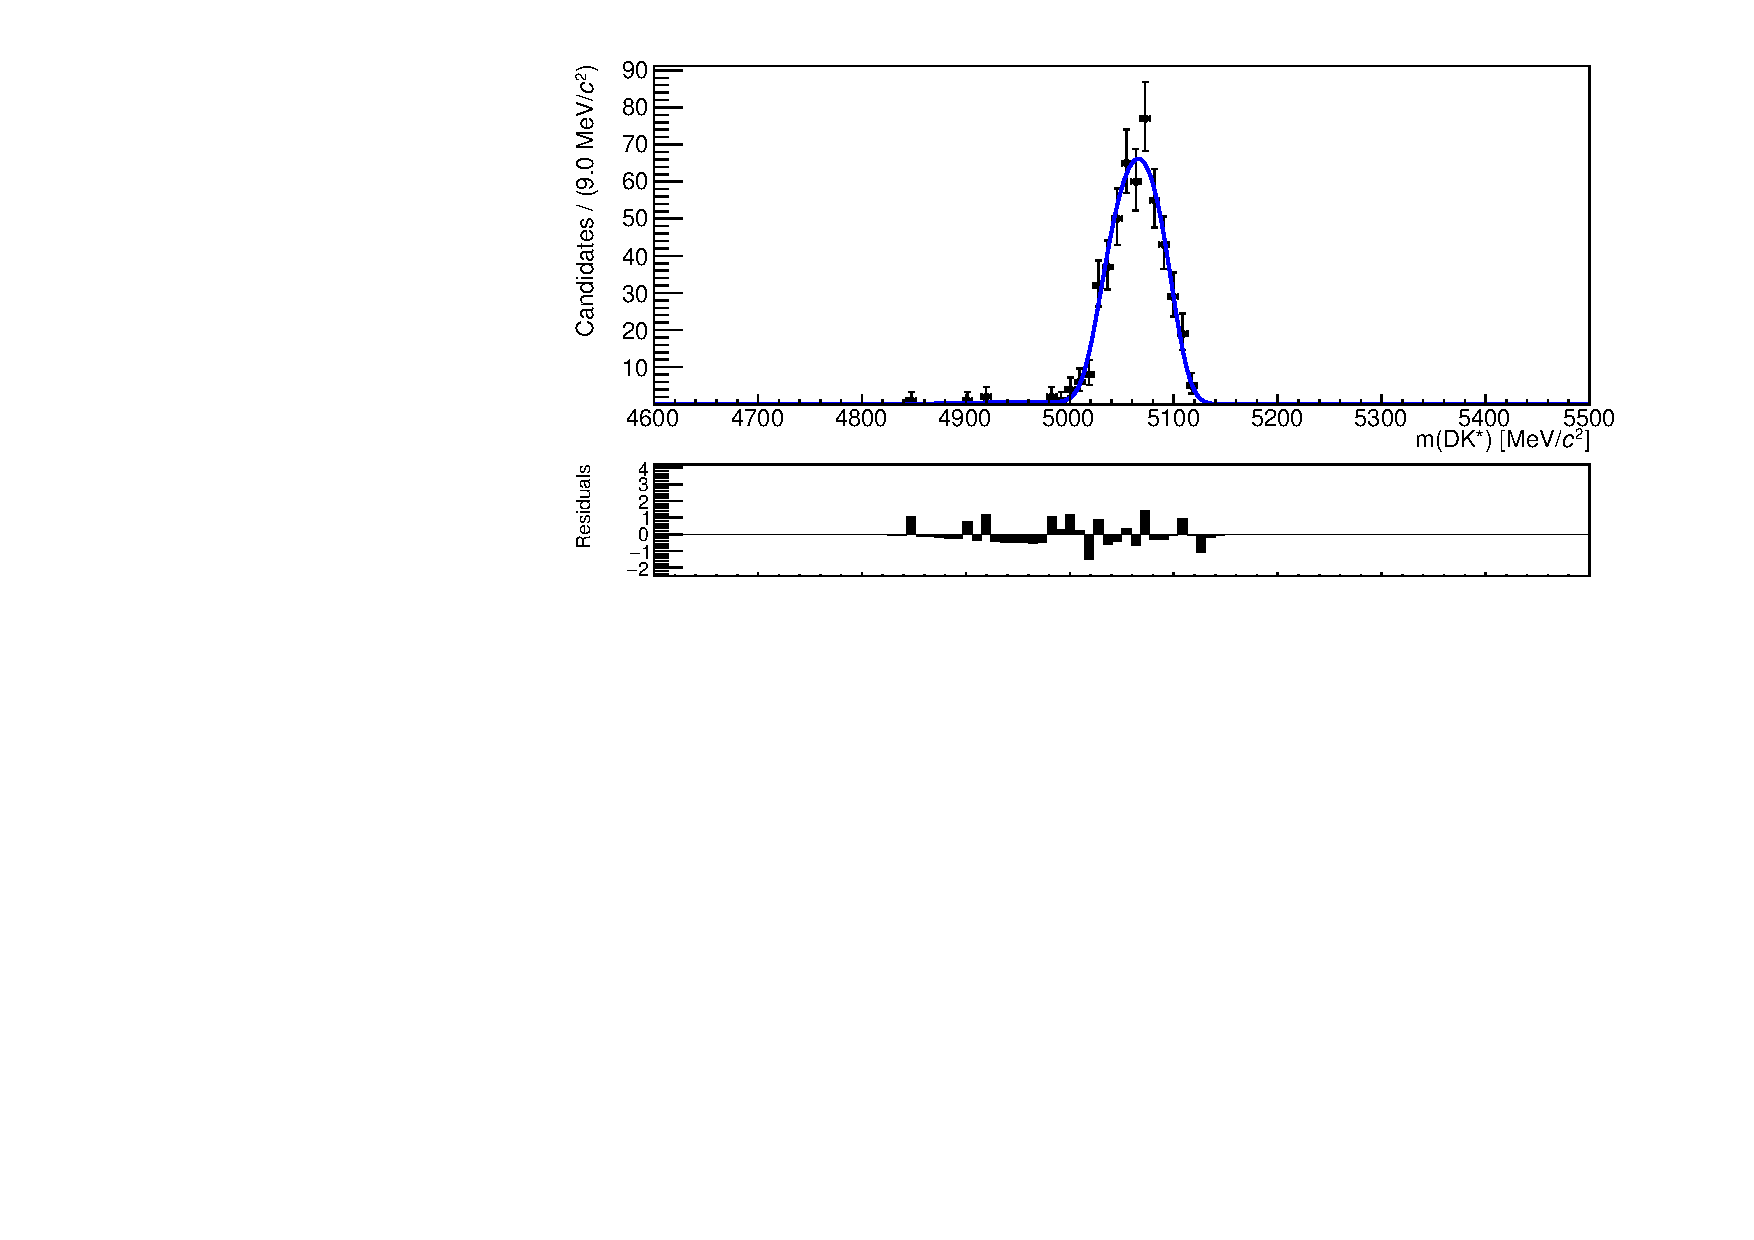
\includegraphics[width=0.5\linewidth]{figures/fitComponents/Bdpi101_LL.pdf}
\put(-180,80) {(f)}
\caption{Fit to $B \to D^*K^*$ \runone simulated samples in all the different modes for LL candidates (a) \decay{\Bm}{(\decay{\Dstarz}{\Dz[\piz]})\Kstarm} 010, (b) \decay{\Bm}{(\decay{\Dstarz}{\Dz[\piz]})\Kstarm} 101, (c) \decay{\Bm}{(\decay{\Dstarz}{\Dz[\gamma]})\Kstarm} 010, (d) \decay{\Bm}{(\decay{\Dstarz}{\Dz[\gamma]})\Kstarm} 101, (e) \decay{\Bd}{(\decay{\Dstarp}{\Dz[\pip]})\Kstarm} 010, and (f) \decay{\Bd}{(\decay{\Dstarp}{\Dz[\pip]})\Kstarm} 101}
\label{partrecofitsLL}
\end{figure}

\begin{figure}[h]
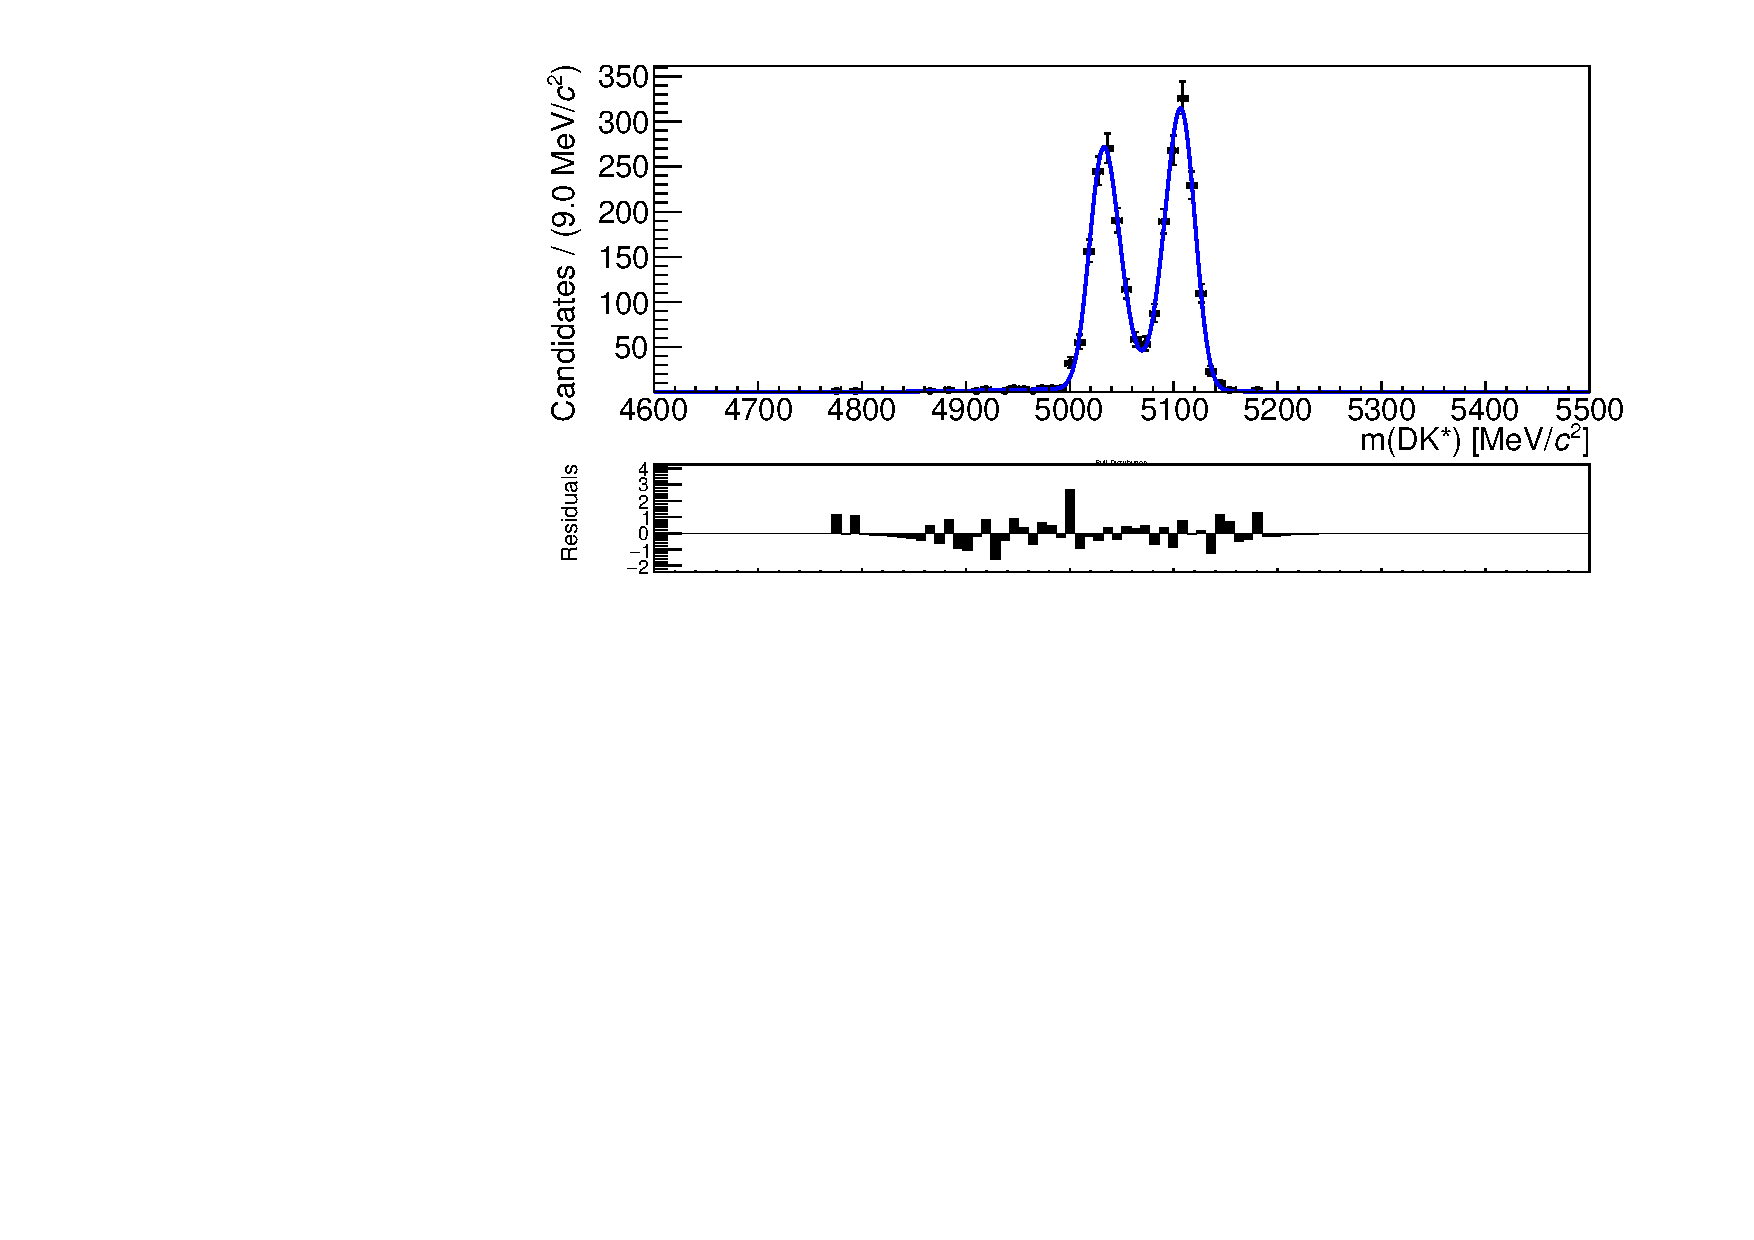
\includegraphics[width=0.5\linewidth]{figures/fitComponents/Bupi010_DD.pdf}
\put(-180,80) {(a)}
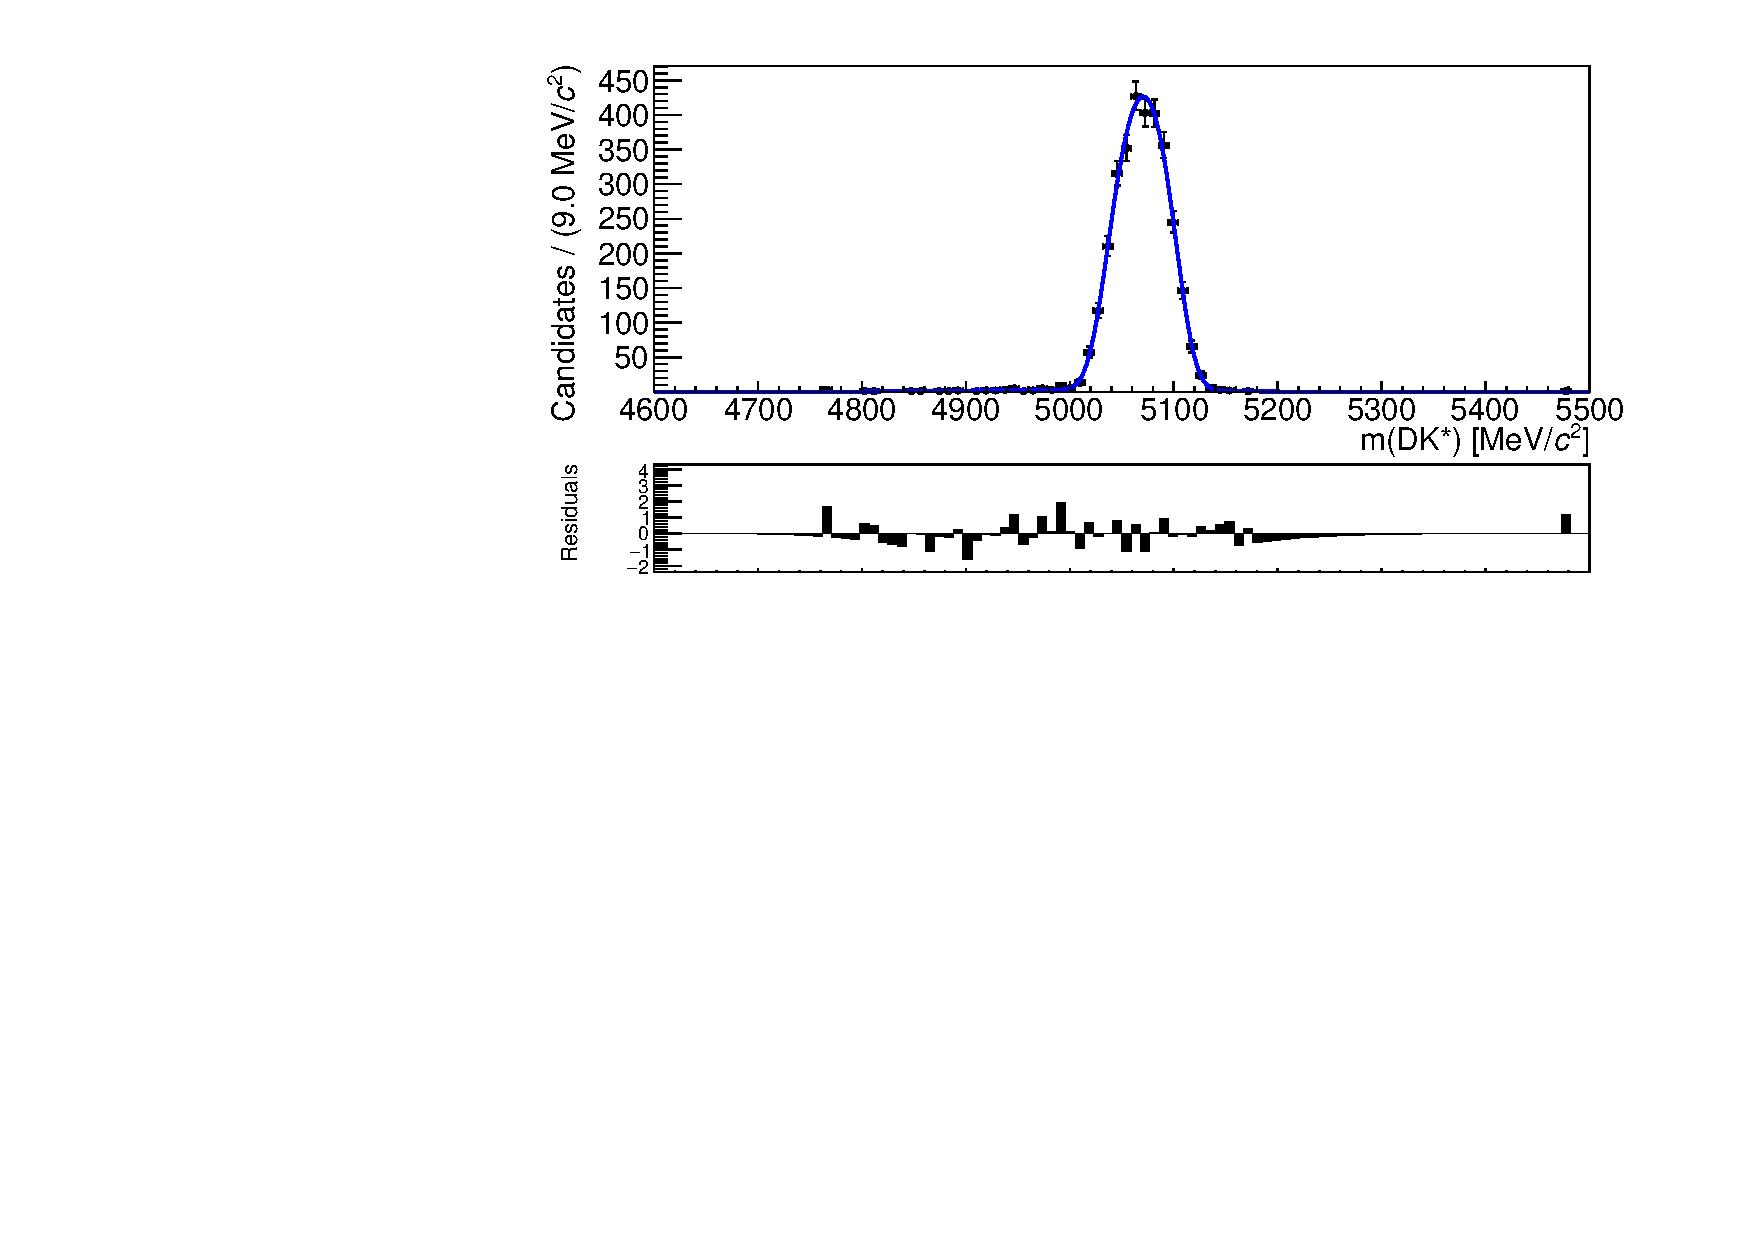
\includegraphics[width=0.5\linewidth]{figures/fitComponents/Bupi101_DD.pdf}
\put(-180,80) {(b)}
\hfill
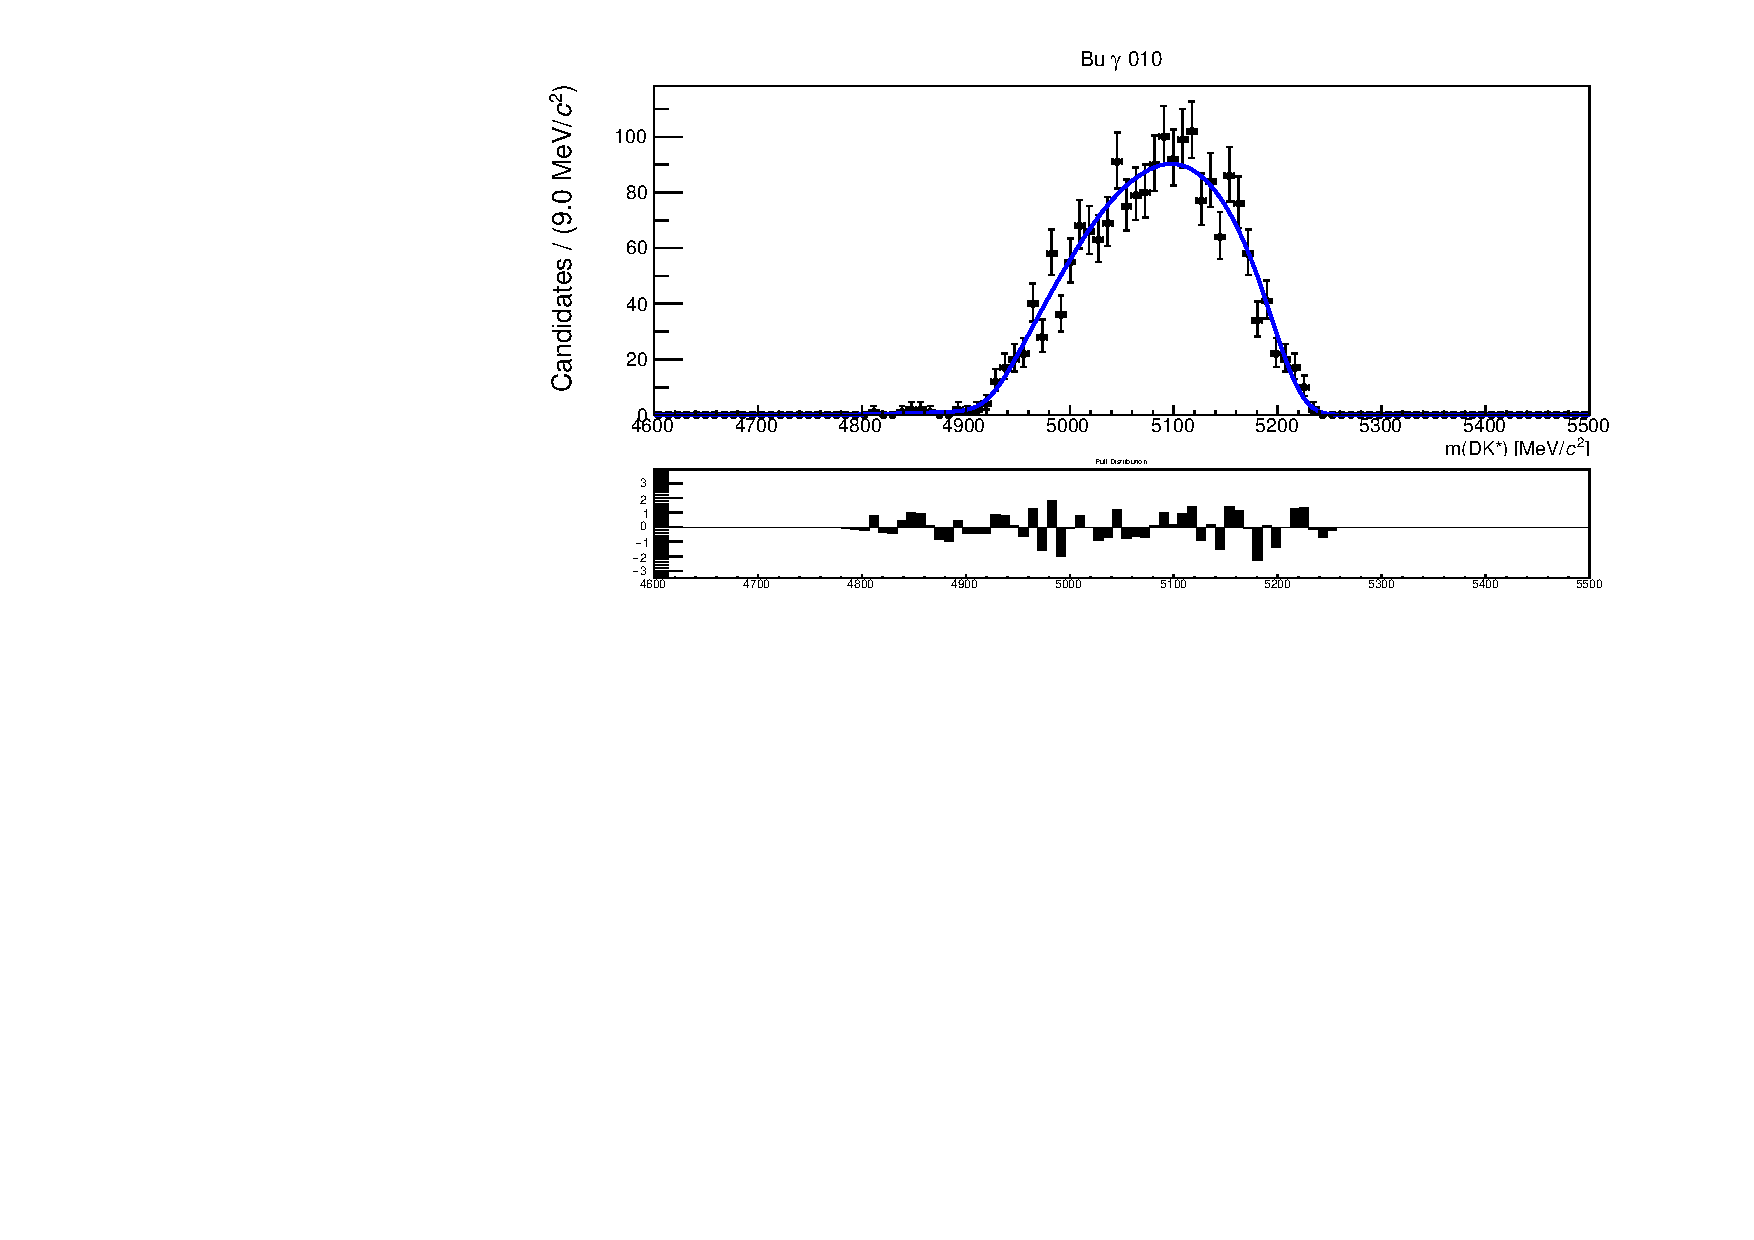
\includegraphics[width=0.5\linewidth]{figures/fitComponents/Bugamma010_DD.pdf}
\put(-180,80) {(c)}
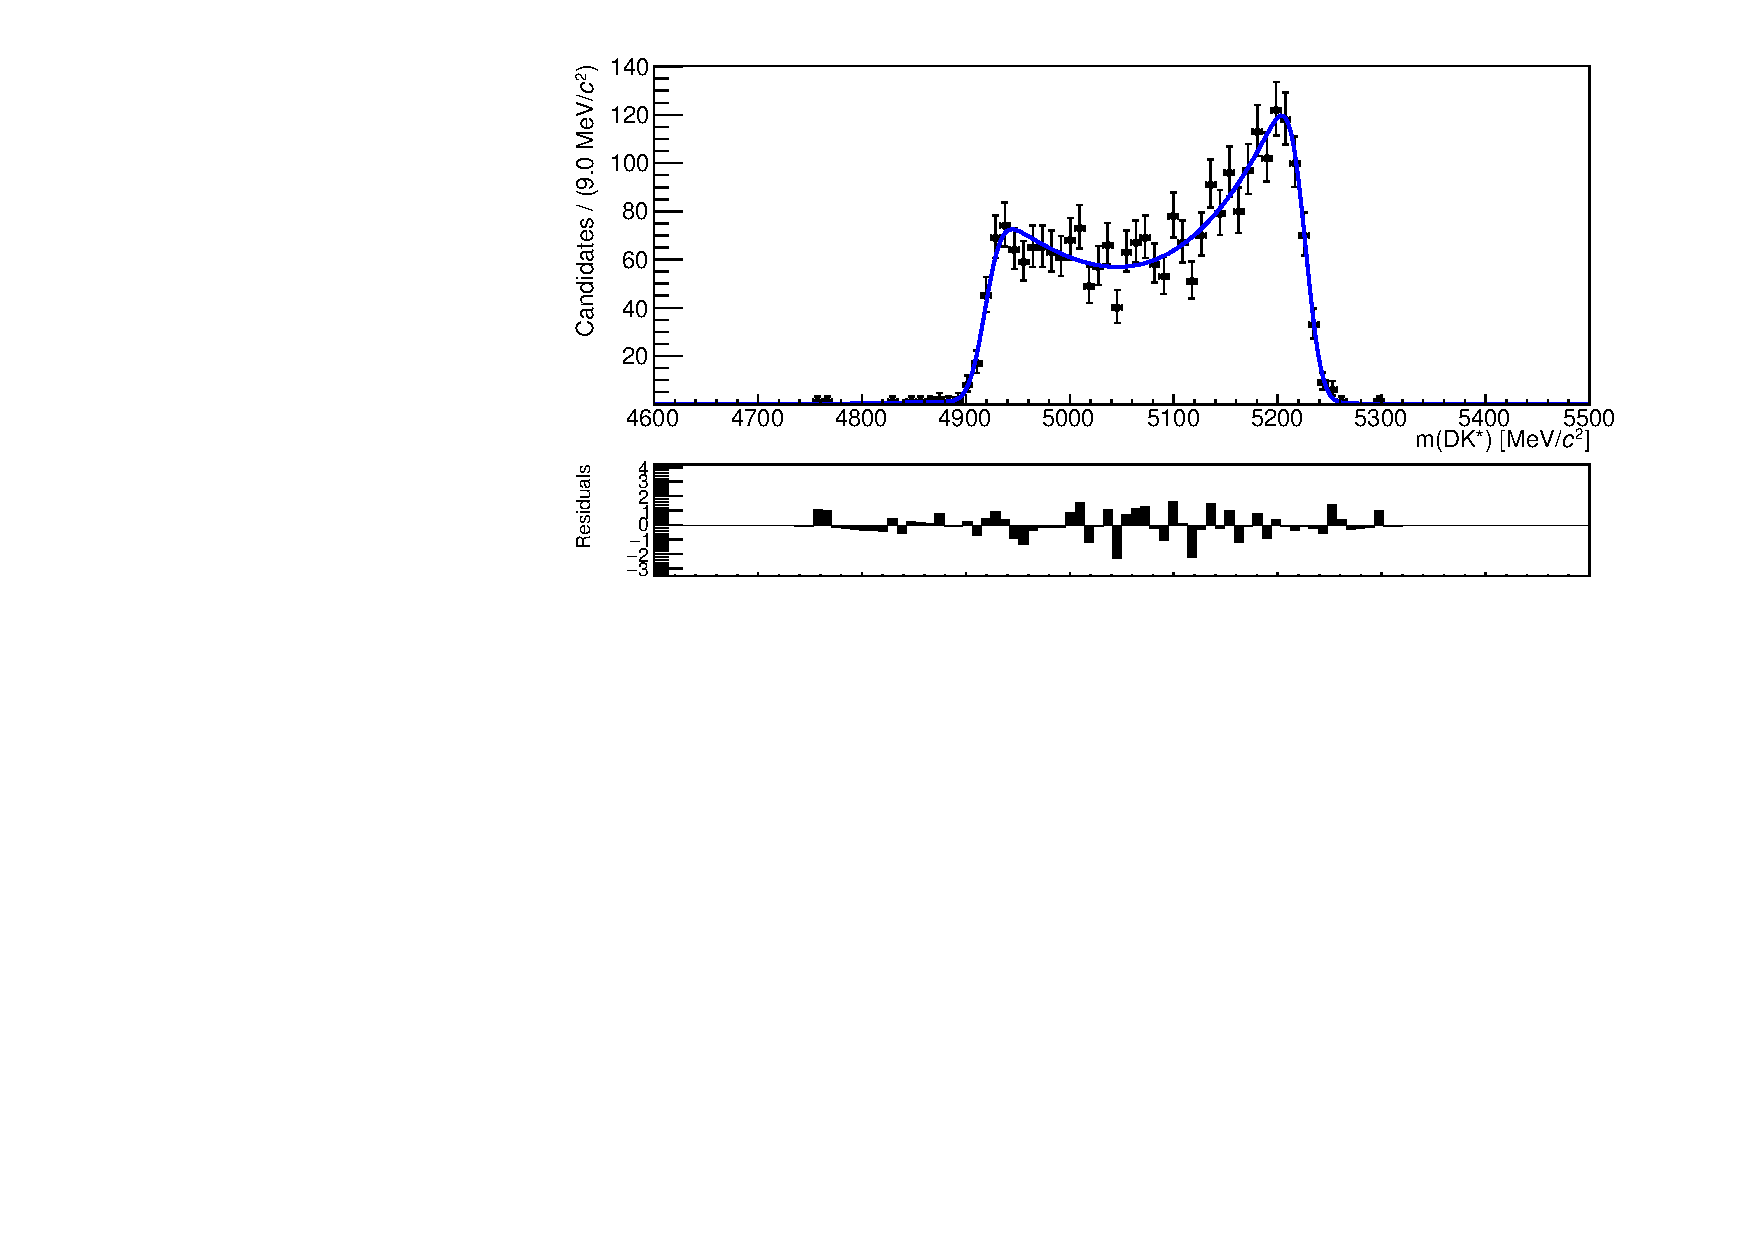
\includegraphics[width=0.5\linewidth]{figures/fitComponents/Bugamma101_DD.pdf}
\put(-180,80) {(d)}
\hfill
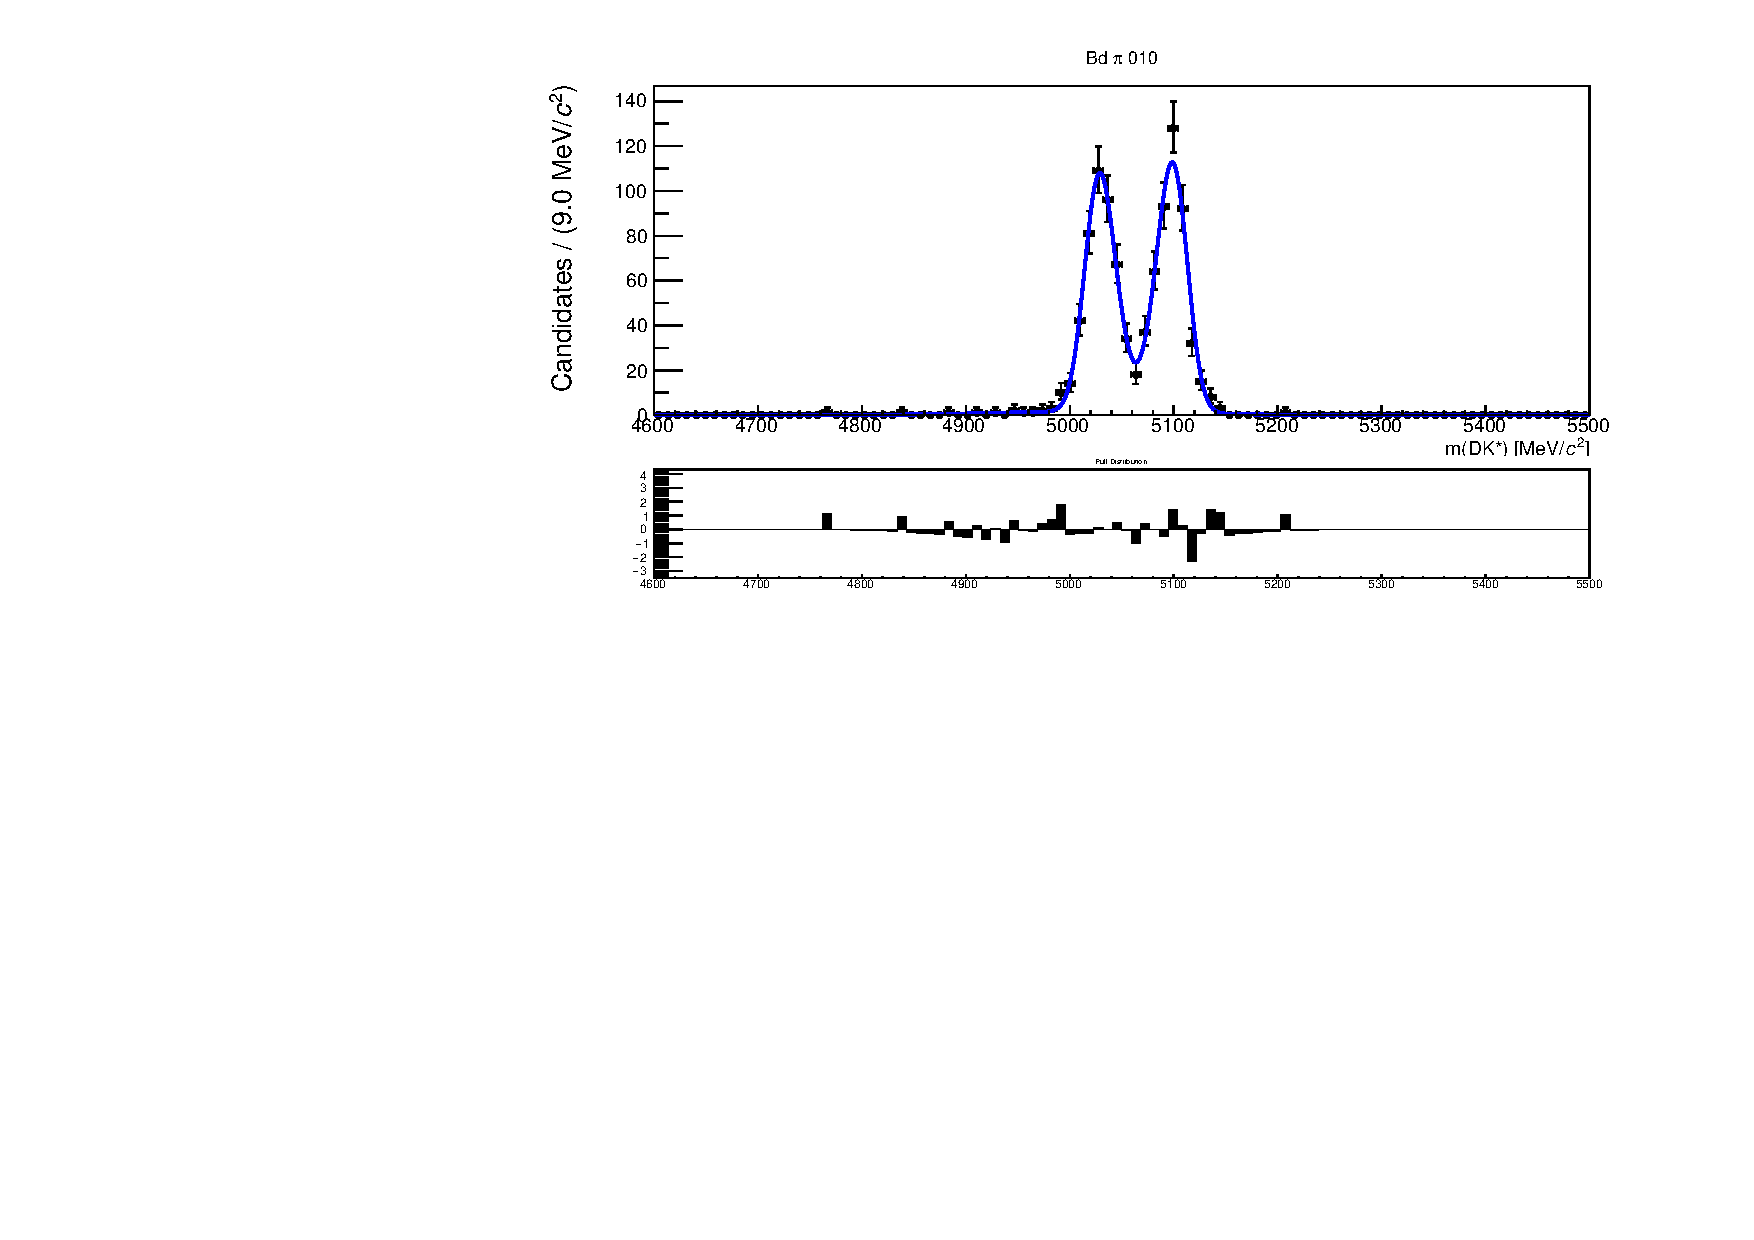
\includegraphics[width=0.5\linewidth]{figures/fitComponents/Bdpi010_DD.pdf}
\put(-180,80) {(e)}
\includegraphics[width=0.5\linewidth]{figures/fitComponents/Bdpi101_DD.pdf}
\put(-180,80) {(f)}
\caption{Fit to $B \to D^*K^*$ \runone simulated samples in all the different modes for DD candidates (a) \decay{\Bm}{(\decay{\Dstarz}{\Dz[\piz]})\Kstarm} 010, (b) \decay{\Bm}{(\decay{\Dstarz}{\Dz[\piz]})\Kstarm} 101, (c) \decay{\Bm}{(\decay{\Dstarz}{\Dz[\gamma]})\Kstarm} 010, (d) \decay{\Bm}{(\decay{\Dstarz}{\Dz[\gamma]})\Kstarm} 101, (e) \decay{\Bd}{(\decay{\Dstarp}{\Dz[\pip]})\Kstarm} 010, and (f) \decay{\Bd}{(\decay{\Dstarp}{\Dz[\pip]})\Kstarm} 101}
\label{partrecofitsDD}
\end{figure}

As there are six shapes in this low mass region of the mass fit, from 4900-5230 MeV, it is necessary to fix some yields in order to have a stable fit. The total partially reconstructed PDF is given in Equation \ref{partrecofunction}.
\begin{equation}
P_{partreco} = f_0P_0 + (1 - f_0)P_{\pm 1}
\label{partrecofunction}
\end{equation}
where $P_0$ and $P_{\pm 1}$, which represent the total PDF for the \Dstar helicity states 0 and $\pm$1 respectively, are given by
\begin{align*}
P_0 &= P^{Bu,\pi}_0 + c^{Bu,\gamma}_0P^{Bu,\gamma}_0 + c^{Bd,\pi}_0P^{Bd,\pi}_0 \\
P_{\pm 1} &= P^{Bu,\pi}_{\pm 1} + c^{Bu,\gamma}_{\pm 1}P^{Bu,\gamma}_{\pm 1} + c^{Bd,\pi}_{\pm 1}P^{Bd,\pi}_{\pm 1} \text{ .}
\end{align*}
The yield ratios between \decay{\Bm}{(\decay{\Dstarz}{\Dz[\piz]})\Kstarm}, \decay{\Bm}{(\decay{\Dstarz}{\Dz[\gamma]})\Kstarm} and \decay{\Bd}{(\decay{\Dstarp}{\Dz[\pip]})\Kstarm} are fixed separately for the 0 and $\pm$1 helicity states of the \Dstar. These yield ratios, $c^{Bu,\gamma}_0$, $c^{Bd,\pi}_0$, $c^{Bu,\gamma}_{\pm 1}$ and $c^{Bd,\pi}_{\pm 1}$, that are fixed in the fit to the values given in Table \ref{fixedyieldratios}, are obtained from a ratio of braching fractions and selection efficiencies, an example calculation is given in Equation \ref{partrecoexample}. This calculation is performed for each of the ratios listed in Table \ref{fixedyieldratios}. Branching fractions for the partially reconstructed decays are given in Table \ref{partrecoBRs}. Simulated events are generated for each of the modes and the values of $\epsilon_{sel}$, used in Equation \ref{partrecoexample}, are given by the fraction of simulated events passing the selection.

\begin{equation}
\frac{N(\decay{\B}{(\decay{\Dstar}{\Dz\piz})\Kstar}\ 010)}{N(\decay{\B}{(\decay{\Dstar}{\Dz\gamma})\Kstar}\ 010)} = \frac{BR(\decay{\B}{(\decay{\Dstar}{\Dz\piz})\Kstar})}{BR(\decay{\B}{(\decay{\Dstar}{\Dz\gamma})\Kstar})} \times \frac{\epsilon_{sel}(\decay{\B}{(\decay{\Dstar}{\Dz\piz})\Kstar}\ 010)}{\epsilon_{sel}(\decay{\B}{(\decay{\Dstar}{\Dz\gamma})\Kstar}\ 010)}
\label{partrecoexample}
\end{equation}

\begin{table}[h]
\centering
\begin{tabular}{c|c}
Mode & Branching ratio \\
\hline
\decay{\Bm}{(\decay{\Dstarz}{\Dz[\piz]})\Kstarm} & $(5.0 \pm 0.9) \times 10^{-4}$ \\
\decay{\Bm}{(\decay{\Dstarz}{\Dz[\gamma]})\Kstarm} & $(3.1 \pm 0.6) \times 10^{-4}$ \\
\decay{\Bd}{(\decay{\Dstarp}{\Dz[\pip]})\Kstarm} & $(2.2 \pm 0.4) \times 10^{-4}$ \\
\end{tabular}
\caption{Branching ratios for the different partially reconstructed decay modes~\cite{PDG2014}}
\label{partrecoBRs}
\end{table}

\begin{table}[h]
\centering
\begin{tabular}{ccc}
\hline
& LL & DD \\
\hline
$c^{Bu,\gamma}_0$ & $0.53 \pm 0.14$ & $0.51 \pm 0.14$ \\[3mm]
$c^{Bd,\pi}_0$ & $0.38 \pm 0.14$ & $0.37 \pm 0.14$ \\[3mm]
$c^{Bu,\gamma}_{\pm 1}$ & $0.53 \pm 0.14$ & $0.51 \pm 0.14$ \\[3mm]
$c^{Bd,\pi}_{\pm 1}$ & $0.38 \pm 0.14$ & $0.38 \pm 0.14$ \\[3mm]
\hline
\end{tabular}
\caption{Yield ratios fixed in the mass fit for the partically reconstructed backgrounds}
\label{fixedyieldratios}
\end{table}

Other backgrounds investigated in this analysis, but not included in the mass fit are discussed in Section \ref{sec:backgrounds}.


\subsection{Mass fit}
\label{sec:massfit:fit}

A fit to the invariant B mass in the $K\pi$ and $K\pi\pi\pi$ favoured mode is performed using the shapes discussed in Sections \ref{sec:massfit:signal}, \ref{sec:massfit:combinatorial} and \ref{sec:massfit:partreco}. The total PDF is given by
\begin{equation}
P_{tot} = N_{sig}P_{sig} + N_{comb}P_{comb} + N_{dstkst}P_{dstkst} \text{ ,}
\end{equation}
where $N_{sig}$, $N_{comb}$ and $N_{dstkst}$ are the yields of the signal, combinatoric and partially reconstructed yields restpectively. The signal PDF, $P_{sig}$, is given by Equation~\ref{DCBshape}, the partially reconstructed PDF, $P_{dstkst}$, is given by Equation~\ref{partrecofunction} and the combintorial PDF is an exponential, $P_{comb} = e^{\beta m}$, where the slope parameter $\beta$ is able to vary in the fit. The yield of the signal and combinatoric shape, $N_{sig}$ and $N_{comb}$, are left to vary without constraint. Other parameters allowed to vary are the mean, $\mu$, and width, $\sigma$, of the signal PDF. The only parameters able to vary in the partially reconstructed background are the yield ratio between the 010 and 101 amplitudes, $f_0$, and the overall yield, $N_{dstkst}$.

Figures \ref{massfitskpi} and \ref{massfitsk3pi} show the fits to the invariant B mass distribution in the $K\pi$ and $K\pi\pi\pi$ favoured mode respectively for LL and DD candidates in both Run 1 and Run 2. The estimated $K\pi$ signal yield extracted from these fits for Run 1 is $220 \pm 16$ for LL and $505 \pm 24$ for DD, and for Run 2 is $388 \pm 21$ for LL and $901 \pm 33$ for DD. The fit results are shown in Table \ref{fitresultskpi}. For the $K\pi\pi\pi$ mode, the estimated signal yield extracted from these fits for Run 1 is $87 \pm 10$ for LL and $205 \pm 16$ for DD, and for Run 2 is $215 \pm 15$ for LL and $516 \pm 25$ for DD. The fit results are shown in Table \ref{fitresultsk3pi}.

\begin{figure}
\centering
\subfloat[Run 1 LL]{\includegraphics[width=0.7\linewidth]{figures/fitComponents/massFit_LL_KPi_run1.pdf}}
\vspace{-12pt}
\hfill
\subfloat[Run 1 DD]{\includegraphics[width=0.7\linewidth]{figures/fitComponents/massFit_DD_KPi_run1.pdf}}
\vspace{-12pt}
\hfill
\subfloat[Run 2 LL]{\includegraphics[width=0.7\linewidth]{figures/fitComponents/massFit_LL_KPi_run2.pdf}}
\vspace{-12pt}
\hfill
\subfloat[Run 2 DD]{\includegraphics[width=0.7\linewidth]{figures/fitComponents/massFit_DD_KPi_run2.pdf}}
\caption{Fits to the invariant B mass distribution in the $K\pi$ favoured mode}
\label{massfitskpi}
\end{figure}

\begin{figure}
\centering
\subfloat[Run 1 LL]{\includegraphics[width=0.7\linewidth]{figures/fitComponents/massFit_LL_KPiPiPi_run1.pdf}}
\vspace{-12pt}
\hfill
\subfloat[Run 1 DD]{\includegraphics[width=0.7\linewidth]{figures/fitComponents/massFit_DD_KPiPiPi_run1.pdf}}
\vspace{-12pt}
\hfill
\subfloat[Run 2 LL]{\includegraphics[width=0.7\linewidth]{figures/fitComponents/massFit_LL_KPiPiPi_run2.pdf}}
\vspace{-12pt}
\hfill
\subfloat[Run 2 DD]{\includegraphics[width=0.7\linewidth]{figures/fitComponents/massFit_DD_KPiPiPi_run2.pdf}}
\caption{Fits to the invariant B mass distribution in the $K\pi$ favoured mode}
\label{massfitsk3pi}
\end{figure}

\begin{table}[h]
\centering
\begin{tabular}{l|cc|cc}
\hline
& \multicolumn{2}{c}{Run 1} & \multicolumn{2}{c}{Run 2} \\
& LL & DD & LL & DD \\
\hline
$\beta$ & $(-4.8 \pm 0.5) \times 10^{-3}$ & $(-2.8 \pm 0.3) \times 10^{-3}$ & $(-4.4 \pm 0.5) \times 10^{-3}$ & $(-2.5 \pm 0.2) \times 10^{-3}$ \\
$f_0$ & $0.15 \pm 0.08$ & $0.12 \pm 0.05$ & $0.18 \pm 0.05$ & $0.06 \pm 0.04$ \\
$\mu$ & $5280.7 \pm 0.8$ & $5280.7 \pm 0.6$ & $5278.5 \pm 0.8$ & $5278.6 \pm 0.5$ \\
$N_{comb}$ & $167 \pm 20$ & $472 \pm 34$ & $223 \pm 24$ & $1100 \pm 50$ \\
$N_{dstkst}$ & $338 \pm 23$ & $810 \pm 36$ & $654 \pm 31$ & $1397 \pm 49$ \\
$N_{sig}$ & $220 \pm 16$ & $505 \pm 24$ & $388 \pm 21$ & $901 \pm 33$ \\
$\sigma$ & $10.2 \pm 0.7$ & $11.5 \pm 0.5$ & $12.2 \pm 0.6$ & $11.5 \pm 0.4$ \\
\hline
\end{tabular}
\caption{Fit results from the $K\pi$ favoured mode for LL and DD candidates, corresponding to the fits in Figure \ref{massfitskpi}. The parameter $\beta$ is the combinatoric background slope, $f_0$ is the yield ratio between 010 and 101 helicity amplitudes, $\sigma$ is the floating width of the signal shape, and $N_{sig}$, $N_{comb}$ and $N_{dstkst}$ are the yields of signal, combinatoric background and partially reconstructed decays respectively}
\label{fitresultskpi}
\end{table}

\begin{table}[h]
\centering
\begin{tabular}{l|cc|cc}
\hline
& \multicolumn{2}{c}{Run 1} & \multicolumn{2}{c}{Run 2} \\
& LL & DD & LL & DD \\
\hline
$\beta$ & $(-5.2 \pm 1.1) \times 10^{-3}$ & $(-2.3 \pm 0.4) \times 10^{-3}$ & $(-4.4 \pm 0.5) \times 10^{-3}$ & $(-2.1 \pm 0.2) \times 10^{-3}$ \\
$f_0$ & $0.26 \pm 0.11$ & $0.20 \pm 0.08$ & $0.15 \pm 0.07$ & $0.16 \pm 0.05$ \\
$\mu$ & $5281.3 \pm 1.3$ & $5283.9 \pm 0.9$ & $5278.7 \pm 1.0$ & $5277.7 \pm 0.7$ \\
$N_{comb}$ & $50 \pm 12$ & $252 \pm 24$ & $168 \pm 20$ & $707 \pm 40$ \\
$N_{dstkst}$ & $154 \pm 15$ & $317 \pm 24$ & $342 \pm 23$ & $914 \pm 40$ \\
$N_{sig}$ & $102 \pm 10$ & $226 \pm 16$ & $244 \pm 16$ & $578 \pm 27$ \\
$\sigma$ & $11.4 \pm 1.0$ & $11.3 \pm 0.8$ & $12.9 \pm 0.8$ & $13.1 \pm 0.6$ \\
\hline
\end{tabular}
\caption{Fit results from the $K\pi\pi\pi$ favoured mode for LL and DD candidates, corresponding to the fits in Figure \ref{massfitsk3pi}. The parameter $\beta$ is the combinatoric background slope, $f_0$ is the yield ratio between 010 and 101 helicity amplitudes, $\sigma$ is the floating width of the signal shape, and $N_{sig}$, $N_{comb}$ and $N_{dstkst}$ are the yields of signal, combinatoric background and partially reconstructed decays respectively}
\label{fitresultsk3pi}
\end{table}

An additional source of background coming from the decay \decay{\Lb}{\Lc(pK\pip)\Kstarm} is included in the fits for the \decay{\Bm}{\D(\Kp\Km)\Kstarm} mode, as discussed in detail in Section \ref{sec:backgrounds:Lb2LcKst}. The yield of \decay{\Lb}{\Lc(pK\pip)\Kstarm} compared to the signal yield in the \decay{\Bm}{\D(\Km\pip)\Kstarm} mode is allowed to vary.

%%%%%%%%%%%%%%%%%%%%%%%%
\subsection{Choice of fit range}
\label{sec:massfit:range}	

Fixing the relative yields for the partially reconstructed shapes, as in Table \ref{fixedyieldratios}, is possible only under the assumption that \CP violation is negligible. This is a fair assumption for the favoured \decay{\Dz}{\Km\pip} decay, however in the other \D modes, for example \decay{\Dz}{\Kp\Km}, there is expected \CP violation for which the parameters are entirely unknown. Therefore, it is not possible make any constraints at all in these modes. The fit that would result from fitting six individual yields with an order of magnitude less data would be unstable and this lack of constraint in the low mass region would lead to a large amount of freedom in the combinatoric, significantly affecting the signal yield. 

The overlap of the partially reconstructed and signal peaks is very small. There are a number of advantages to raising the lower range of the mass parameterisation up to 5230 \mev, which only removes 0.4\% of signal. The advantages include avoiding the need to fit the various partially reconstructed yields in each of the other D decays modes. These cannot use the same assumptions and fractions as determined in the Cabibbo-favoured mode due to expected CP violation. Further benefits are that low level broad backgrounds that may be present in the range 4900 - 5200 \mev do not need to considered as sources of systematics uncertainty. The shape and yield of the small amount of partially reconstructed background present in all \D decay categories above 5230 \mev is determined and fixed from the fit of data with the Cabibbo-favoured decay, taking into account the smaller branching fractions of the $D$ decays. It is less than an event for all the CP violating modes. Due to the assumptions present in the initial fit, uncertainties in the yield and shape and possible asymmetries in distribution between \Bp and \Bm are evaluated as systematic uncertainties. This systematic uncertainty is dealt with in Section \ref{sec:systematics:partreco}.


\clearpage
